\documentclass[twoside,a4paper,11pt]{memoir}
\usepackage{preamble/a4}
\usepackage{times}
\usepackage{pslatex}
\usepackage{url}
\usepackage{preamble/mscthesis}
\usepackage{preamble/lipsum} % standard filler text, only needed for demo
\usepackage{amsmath}
\usepackage{amssymb}
\usepackage{amsthm}
\usepackage{longtable}

% \newtheorem{definition}{Definition}
\theoremstyle{plain}
\newtheorem{theorem}{Theorem}[chapter]
\newtheorem{proposition}[theorem]{Proposition}
\newtheorem{lemma}[theorem]{Lemma}
\newtheorem{corollary}[theorem]{Corollary}

\theoremstyle{definition}
\newtheorem{definition}[theorem]{Definition}

\theoremstyle{remark}
\newtheorem{remark}[theorem]{Remark}

% %% The package 'algorithm' is useful, but incompatible with memoir.
% %% Cor-Paul Bezemer / http://homes.esat.kuleuven.be/~dvherten/esatthesis.html
% %% suggest the following fix:
\let\newfloat\undefined \usepackage{algorithmic} 
\usepackage{algorithm}

% % Include right (LaTeX/PDFLaTeX) graphics package
% % (doesn't work under cygwin apperently)
% %\ifx\pdftexversion\undefined
% \usepackage[dvips]{graphicx}
%
% \usepackage[dvips]{color}
% %\else
% %\usepackage[pdftex]{graphicx}
% %\usepackage[pdftex]{color}
% %\fi
\usepackage{ifpdf}

\ifpdf
  \usepackage{graphicx}
  \usepackage{xcolor}
\else
  \usepackage[dvips]{graphicx}
  \usepackage[dvips]{xcolor}
\fi

\usepackage{hyperref}
\usepackage{subcaption}

% Used in the bibliography to enable \citeauthor{citation}
\usepackage[round]{natbib}

% Add for highlighting changes
% \newenvironment{revblock}{\begingroup\color{blue}}{\endgroup}
% \newcommand{\rev}[1]{{\color{blue}#1}}

% Change the above to this to remove highlighting
\newenvironment{revblock}{}{}
\newcommand{\rev}[1]{#1}

% Ensure that urls longer than the page width are broken up
% Based on the answer of StackOverflow user "xamde":
% https://tex.stackexchange.com/a/10401/155506
\expandafter\def\expandafter\UrlBreaks\expandafter{\UrlBreaks%  save the current one
  \do\a\do\b\do\c\do\d\do\e\do\f\do\g\do\h\do\i\do\j%
  \do\k\do\l\do\m\do\n\do\o\do\p\do\q\do\r\do\s\do\t%
  \do\u\do\v\do\w\do\x\do\y\do\z\do\A\do\B\do\C\do\D%
  \do\E\do\F\do\G\do\H\do\I\do\J\do\K\do\L\do\M\do\N%
  \do\O\do\P\do\Q\do\R\do\S\do\T\do\U\do\V\do\W\do\X%
  \do\Y\do\Z}

%---------------------------------------------------------------------%
%                     Options                                         %    
%---------------------------------------------------------------------%

\title{Training Dynamics of Overparameterized Neural Networks: A Study of Spectral Bias on $S^1$}
\subtitle{Version of \today}
% The final version of your thesis should typically use a different
% subtitle without the current date, for example
%\subtitle{Master's Thesis} 
% or remove the subtitle by uncommenting the following line: 
%\subtitle{}

\author{Shreyas Kalvankar}                               % CHANGE TO YOUR NAME
\authoremail{\url{skalvankar@tudelft.nl}}       % CHANGE TO YOUR EMAIL ADDRESS
\birthplace{Nashik, India}                % CHANGE TO YOUR BIRTH PLACE
\studentid{6255191}                              % CHANGE TO YOUR STUDENT ID

% Optional for work done at a company, put this in comments if you did
% not do your thesis work at a company
% \company{
% 
\includegraphics[height=2cm]{img/hilbert.ps}\\
% Some Company\\
% With it's address\\
% ThePlace, the Netherlands\\
% \url{www.url.nl}
% }

% Optional (postscript) cover picture. Put this in comments when not needed.
\coverpicture{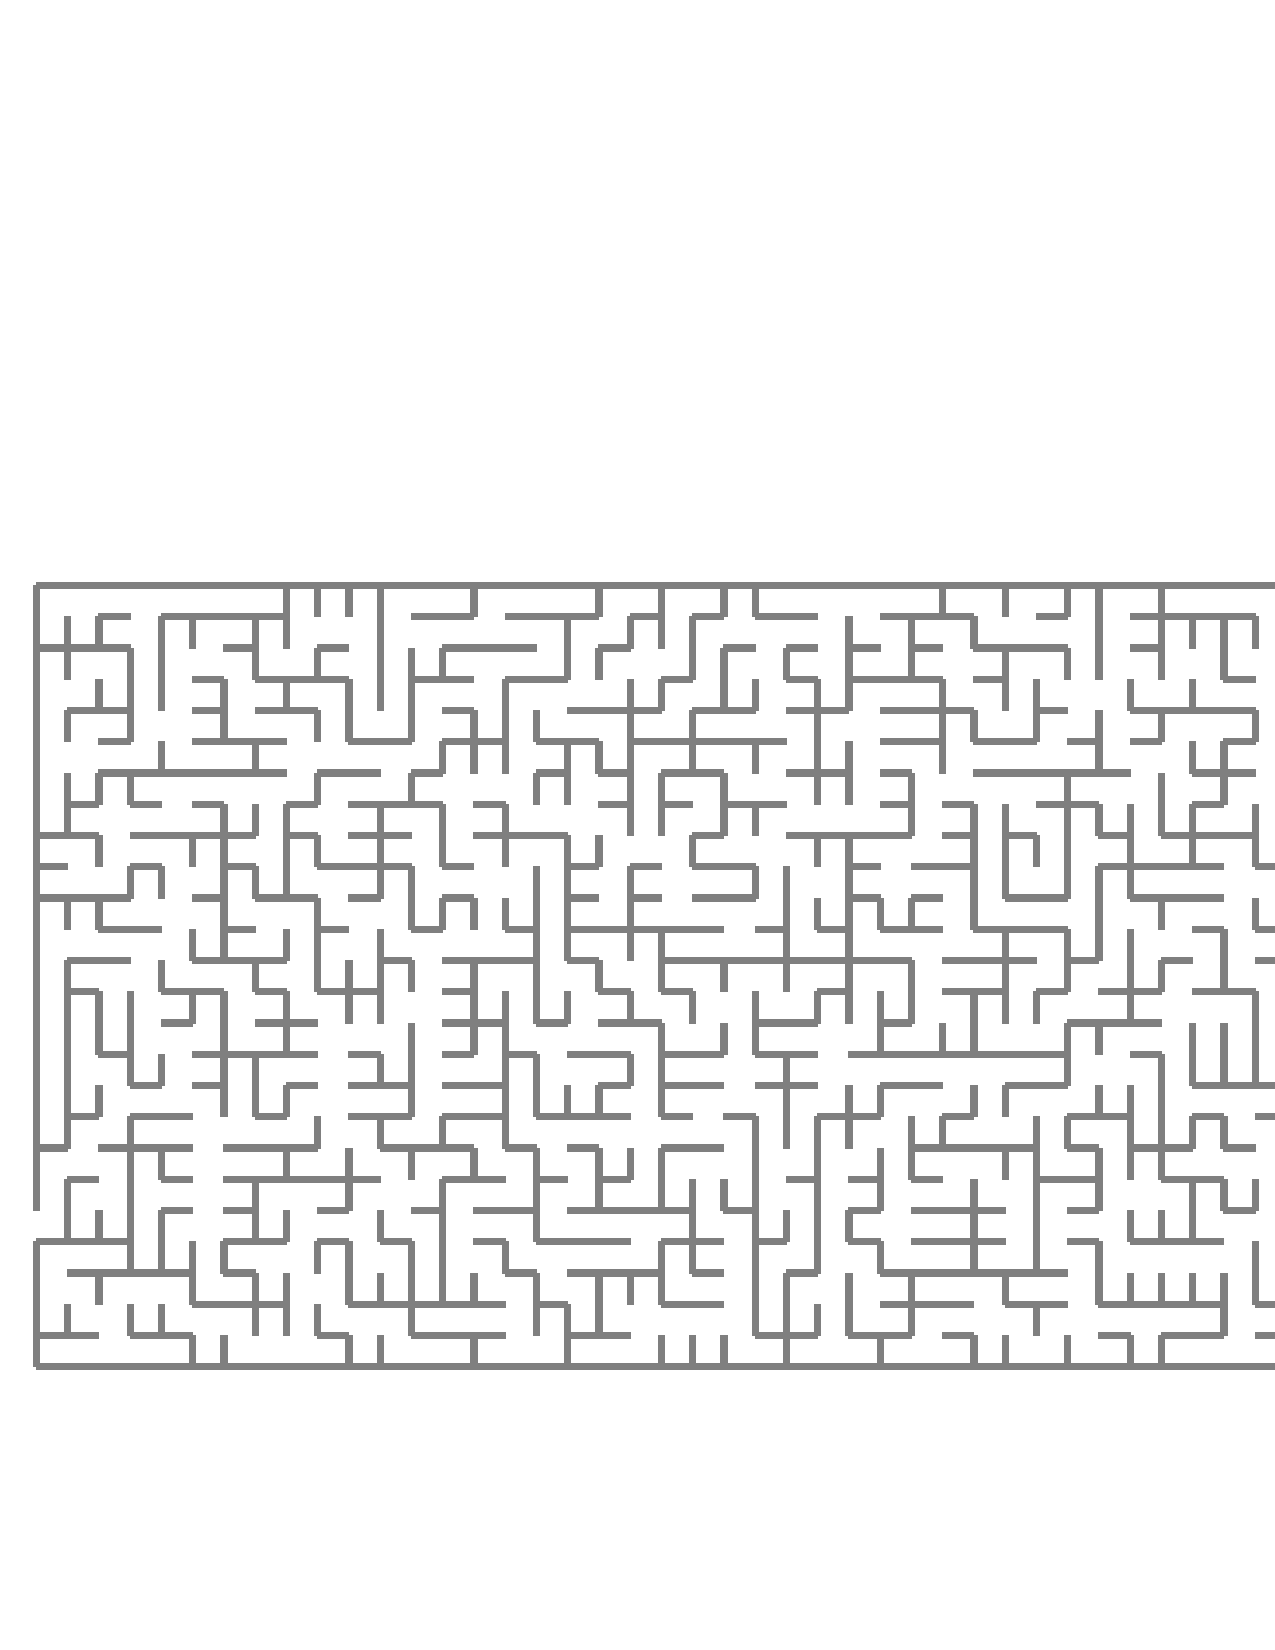
\includegraphics[width=13cm]{../img/maze.pdf}}


% A copyright notice and maybe something about the cover picture
% Put in comments to get the default copyright notice
\colophon{\noindent\copyright{} \the\year{} \theauthor. All rights reserved.}

% thesis committee:
\chair{Prof. Dr. D. M. J. Tax, PRB Group, Faculty EEMCS, TU Delft}
\supervisor{Prof. Dr. A. Heinlein, DIAM, Faculty EEMCS, TU Delft}
% \supervisor{Dr. F. Bartolucci, Faculty EEMCS, TU Delft}
% The following two are optional for LaTeX (current university
% regulations state that at least one of them should be assigned)
% \externalsupervisor{Drs. E.X. Ternal, Some Company}
\committeemember{Prof. Dr. A. Papapanteleon, DIAM, Faculty EEMCS, TU Delft}


\setcounter{tocdepth}{1}
\setsecnumdepth{subsection}
\maxsecnumdepth{subsection}

\begin{document}
\frontmatter
\thispagestyle{empty}
% \maketitle                                      % for the cover page
\makeformaltitlepages{% This thesis studies the training dynamics of overparameterized neural networks
% through spectral bias, the tendency of gradient-based training to learn
% low-frequency components of a target function before high-frequency ones. The
% setting is regression on the unit circle with a one-hidden-layer ReLU network and
% targets given by finite Fourier mixtures, chosen because it is simple enough for
% the dynamics to be written down explicitly yet rich enough to exhibit spectral
% bias.
%
% In the infinite-width limit the residual dynamics are governed by the neural
% tangent kernel. Under the uniform measure on the circle this operator is a
% convolution, so it is diagonalised by the Fourier basis, each frequency decays at
% a rate set by its own eigenvalue, and low frequencies are learned faster because
% their eigenvalues are larger. This gives an explicit reference model for spectral
% bias against which finite effects can be measured.
%
% We then ask how much of this picture survives away from the idealised limit,
% working throughout on a fixed low-frequency Fourier subspace. Replacing the
% uniform measure by finitely many sampled points, we prove non-asymptotic bounds
% showing that the sampled operator stays close to the continuum Fourier prediction,
% with error of order \(O(n^{-1/2})\) in the sample size. Freezing the tangent
% kernel at finite width, we prove an analogous concentration around the
% infinite-width operator at rate \(O(m^{-1/2})\) in the width. In both cases the
% Fourier description degrades gracefully rather than breaking, and the perturbation
% shrinks as the sample size or width grows.
%
% The fixed-kernel account stops once the kernel is allowed to evolve during
% training. Here our analysis is empirical: at small width the evolving kernel
% reaches a lower loss than the frozen one, and it does so not by aligning its
% eigenspaces more closely with the Fourier basis, which can in fact degrade, but by
% increasing the spectral strength of the lowest-frequency blocks. Training therefore
% reshapes the kernel in a direction that reinforces the low-frequency bias rather
% than merely approximating the fixed-kernel dynamics, an effect that diminishes as
% width grows and the kernel moves less. We give evidence that this reweighting is
% tied to the network's parameterisation, since the constant and first-frequency
% modes are the ones the input embedding and bias represent most directly. A formal
% theory of this evolving-kernel regime remains the main problem left open.

In this thesis, we study spectral bias, the tendency of gradient-based training to
learn the low-frequency part of a target before its high-frequency part. We work
in a setting simple enough to analyse explicitly: regression on the unit circle
with a shallow ReLU network. In the infinite-width limit, the residual dynamics
are governed by the Neural Tangent Kernel. Under the uniform measure on the
circle this kernel depends only on the angle between two points, so the
associated operator is a convolution and the Fourier modes are its
eigenfunctions, each decaying at a rate set by its eigenvalue, and the lower the
frequency, the larger the eigenvalue, so low frequencies are learned first.

Away from this idealised limit the picture degrades only gradually. On a fixed
low-frequency subspace, both finite sampling and frozen finite width keep the
operator close to the continuum Fourier prediction, with error of order
\(O(n^{-1/2})\) in the sample size \(n\) and \(O(m^{-1/2})\) in the width \(m\).
The description breaks only once the kernel is allowed to evolve during training.
At small width the evolving kernel reaches a lower loss by strengthening its
lowest-frequency components, even as its alignment with the Fourier basis fails
to improve. This reinforces the low-frequency bias rather than approximating the
fixed-kernel dynamics. A formal theory of this evolving-kernel regime remains the
main open problem.
}         % for formal title pages with all info

\include{frontmatter/preface} % ---------------------------------------------------------------------
%  Notation
%
%  Suggested placement: in the frontmatter, after the preface and before
%  the table of contents. In thesis.tex, add (inside \frontmatter):
%
%      % ---------------------------------------------------------------------
%  Notation
%
%  Suggested placement: in the frontmatter, after the preface and before
%  the table of contents. In thesis.tex, add (inside \frontmatter):
%
%      % ---------------------------------------------------------------------
%  Notation
%
%  Suggested placement: in the frontmatter, after the preface and before
%  the table of contents. In thesis.tex, add (inside \frontmatter):
%
%      \include{frontmatter/notation}
%
%  This uses only the longtable environment from the `longtable` package.
%  Add \usepackage{longtable} to the preamble if it is not already loaded
%  (amsmath/amssymb are already loaded in thesis.tex).
% ---------------------------------------------------------------------

\chapter*{Notation}
\addcontentsline{toc}{chapter}{Notation}
\markboth{Notation}{Notation}

The following list summarizes the notation used throughout this thesis. Symbols
are grouped by theme and, within each group, ordered roughly by first
appearance. Page or equation references are given where a symbol is formally
defined. Throughout, the circle angle is written $\theta$ in the introductory
linear-model discussion (Chapter~\ref{cha:intro}) and $\varphi$ from the
methodology onward (Chapters~\ref{cha:methodology}--\ref{cha:results}); the two
denote the same angular coordinate on $S^1$.

\vspace{1em}

\begin{longtable}{p{0.26\textwidth} p{0.68\textwidth}}

% ----------------------------------------------------------------
\multicolumn{2}{l}{\textbf{Sets, spaces, and measures}}\\[0.3em]
\endfirsthead
\multicolumn{2}{l}{\small\itshape (Notation, continued)}\\[0.3em]
\endhead

$\mathbb{R},\ \mathbb{Z}$ & The real numbers and the integers. \\[0.4em]
$\mathbb{R}^{d}$ & $d$-dimensional Euclidean space. \\[0.4em]
$S^1$ & The unit circle, identified with the angular domain $\Omega=[0,2\pi)$ and embedded in $\mathbb{R}^2$ via $x(\varphi)=(\cos\varphi,\sin\varphi)$. \\[0.4em]
$S^{d-1}$ & The unit sphere in $\mathbb{R}^d$ (the $(d-1)$-sphere). \\[0.4em]
$\mathcal{X},\ \mathcal{Y}$ & Input space ($\mathcal{X}\subseteq\mathbb{R}^d$) and target space (e.g.\ $\mathcal{Y}=\mathbb{R}^n$ in regression, $\mathcal{Y}=\{1,\dots,C\}$ in classification). \\[0.4em]
$\rho$ & Joint data distribution over $\mathcal{X}\times\mathcal{Y}$; also used for the uniform input distribution. \\[0.4em]
$\mu$ & Uniform probability measure on $S^1$, $d\mu(\varphi)=d\varphi/(2\pi)$. \\[0.4em]
$L^2(\mu)$ & Space of square-integrable functions on $S^1$ with respect to $\mu$, with inner product $\langle\cdot,\cdot\rangle_{L^2(\mu)}$. \\[0.4em]
$\mathcal{H}$ & A reproducing kernel Hilbert space (RKHS). \\[0.4em]
$\mathcal{H}_\theta$ & Tangent parameter space ($\mathbb{R}^p$ in finite dimension; its limit in the infinite-width case). \\[0.4em]
$\Omega$ & The angular domain $[0,2\pi)$; in the mean-field discussion, the neuron parameter space $\mathbb{R}\times\mathbb{R}^d$. \\[0.4em]
$\|\cdot\|_2,\ \|\cdot\|_F,\ \|\cdot\|_{\max}$ & Euclidean ($\ell^2$) norm, Frobenius norm, and entrywise max norm, respectively. \\[0.4em]
$\langle\cdot,\cdot\rangle$ & Euclidean / Hilbert-space inner product. \\[0.4em]
$\mathbb{E},\ \mathbb{P}$ & Expectation and probability. \\[0.4em]
$\mathcal{N}(0,\sigma^2)$ & Gaussian distribution with mean $0$ and variance $\sigma^2$; $I_d$ denotes the $d\times d$ identity. \\[0.6em]

% ----------------------------------------------------------------
\multicolumn{2}{l}{\textbf{Network, data, and training}}\\[0.3em]
$f(x;\theta),\ f_\theta$ & Neural network output at input $x$ with parameter vector $\theta$. \\[0.4em]
$f_m(x;\theta)$ & One-hidden-layer ReLU network of width $m$ in NTK parameterization, $f_m(x;\theta)=\tfrac{1}{\sqrt{m}}\sum_{i=1}^m a_i\,\sigma(w_i^\top x+b_i)$. \\[0.4em]
$\theta$ & Parameter vector, $\theta\in\mathbb{R}^p$; $\theta_0$ its value at initialization. \\[0.4em]
$p$ & Number of network parameters. \\[0.4em]
$m$ & Network width (number of hidden units); also $w$ as a width label in figures. \\[0.4em]
$d$ & Input dimension; also the dimension $d=2K+1$ of the truncated Fourier block $\mathcal{H}_K$. \\[0.4em]
$a_i,\ w_i,\ b_i$ & Output weight, input weight vector, and bias of hidden unit $i$; initialized $a_i\sim\mathcal{N}(0,1)$, $w_i\sim\mathcal{N}(0,I_2)$, $b_i(0)=0$. \\[0.4em]
$v_\alpha,\ w_\alpha$ & Second-layer and first-layer parameters of neuron $\alpha$ in the generic two-layer network. \\[0.4em]
$\sigma,\ \varphi(\cdot)$ & Activation function; $\sigma(t)=t_+=\max\{t,0\}$ is ReLU ($\varphi$ also denotes a generic activation, and elsewhere the circle angle). \\[0.4em]
$W,\ v$ & Hidden-layer weight matrix and output-weight vector of a two-layer network. \\[0.4em]
$\odot$ & Hadamard (elementwise) product. \\[0.4em]
$\mathcal{D}=\{(x_i,y_i)\}_{i=1}^n$ & Training dataset of $n$ i.i.d.\ samples. \\[0.4em]
$n$ & Number of training samples / sampled points. \\[0.4em]
$X$ & Data matrix ($X\in\mathbb{R}^{d\times n}$, columns $x_i$). \\[0.4em]
$y$ & Vector / function of targets. \\[0.4em]
$\ell(\cdot,\cdot)$ & Loss function. \\[0.4em]
$\mathcal{L},\ L$ & Empirical (least-squares) risk; $\mathcal{L}_\rho$ denotes the population risk. \\[0.4em]
$\eta$ & Gradient-descent step size / learning rate. \\[0.4em]
$t,\ k$ (subscript) & Training time / iteration index. \\[0.4em]
$\nabla_\theta$ & Gradient with respect to $\theta$; $\dot{(\cdot)}$ denotes time derivative under gradient flow. \\[0.4em]
$\theta^\star,\ w^\star,\ f^\star$ & Minimizers / fixed points of the relevant objective. \\[0.4em]
$A^{+},\ A^{\ast}$ & Moore--Penrose pseudoinverse and adjoint of an operator/matrix $A$. \\[0.4em]
$\mathrm{range}(\cdot),\ \ker(\cdot)$ & Range (column space) and kernel (null space) of an operator. \\[0.4em]
$\lambda_{\max}(\cdot)$ & Largest eigenvalue of a matrix. \\[0.6em]

% ----------------------------------------------------------------
\multicolumn{2}{l}{\textbf{Neural Tangent Kernel and operators}}\\[0.3em]
$\phi(x),\ \Phi_t(x)$ & Tangent feature map $\nabla_\theta f(x;\theta_0)$ (and its time-$t$ version). \\[0.4em]
$\Theta_0(x,x')$ & Neural Tangent Kernel at initialization, $\nabla_\theta f(x;\theta_0)^\top\nabla_\theta f(x';\theta_0)$. \\[0.4em]
$\Theta_t,\ \Theta_t^{(m)}$ & NTK at training time $t$ (the empirical, width-$m$ kernel). \\[0.4em]
$\Theta_0^{(m)}$ & Finite-width empirical NTK at initialization. \\[0.4em]
$\bar\Theta,\ \Theta$ & Limiting (infinite-width) deterministic NTK; also written as the Gram matrix $\bar\Theta=(\bar\Theta(x_i,x_j))_{i,j}$. \\[0.4em]
$\Theta(\delta)$ & Limiting NTK on $S^1$ as a function of the angular distance $\delta=d(\varphi,\psi)\in[0,\pi]$. \\[0.4em]
$\Theta^{(\mathrm{nb})}$ & Limiting NTK with the trainable hidden-bias contribution removed. \\[0.4em]
$\Theta^{(r)},\ \psi_r$ & One-neuron kernel contribution and one-neuron tangent feature of neuron $r$. \\[0.4em]
$J_0$ & Jacobian of network outputs w.r.t.\ parameters at initialization; $\bar\Theta=J_0 J_0^\ast$. \\[0.4em]
$T_{\bar\Theta},\ T,\ T_\infty$ & Integral operator on $L^2(\mu)$ induced by the limiting kernel; $T_\infty=\lim_{m\to\infty}T_0^{(m)}$. \\[0.4em]
$T_t^{(m)},\ T_0^{(m)}$ & Empirical tangent integral operator at time $t$ and at initialization (frozen operator). \\[0.4em]
$T^{(r)}$ & One-neuron integral operator; $T_0^{(m)}=\tfrac1m\sum_{r=1}^m T^{(r)}$. \\[0.4em]
$T_p$ & Density-weighted integral operator for a non-uniform input density $p(\theta)$. \\[0.4em]
$\kappa$ & The $2\pi$-periodic kernel profile with $\bar\Theta(\theta,\theta')=\kappa(\theta-\theta')$; also a uniform kernel bound and (in the conditioning discussion) a matrix condition number. \\[0.4em]
$r_t,\ r$ & Residual $f_t-y$ (function or vector). \\[0.6em]

% ----------------------------------------------------------------
\multicolumn{2}{l}{\textbf{Fourier basis, spectrum, and subspaces}}\\[0.3em]
$\theta,\ \varphi,\ \gamma$ & Angular coordinate on $S^1$; $\gamma$ is used as the angle variable in target functions. \\[0.4em]
$\phi_q(\theta)=e^{iq\theta}$ & Complex Fourier mode of frequency $q\in\mathbb{Z}$. \\[0.4em]
$\phi_0,\ \phi_{k,c},\ \phi_{k,s}$ & Real Fourier basis of $L^2(\mu)$: $\phi_0=1$, $\phi_{k,c}=\sqrt{2}\cos(k\varphi)$, $\phi_{k,s}=\sqrt{2}\sin(k\varphi)$. \\[0.4em]
$\psi_j$ & Generic orthonormal eigenfunction of an integral operator. \\[0.4em]
$k,\ q$ & Fourier frequency index; $k(p)$ is the frequency of basis function $\phi_p$. \\[0.4em]
$K$ & Frequency cutoff defining the retained low-frequency block. \\[0.4em]
$\mathcal{H}_K$ & Truncated Fourier subspace $\operatorname{span}\{\phi_0,\phi_{k,c},\phi_{k,s}:1\le k\le K\}$, of dimension $d=2K+1$. \\[0.4em]
$\mathcal{F}_k$ & Frequency-$k$ subspace: $\mathcal{F}_0=\operatorname{span}\{\phi_0\}$, $\mathcal{F}_k=\operatorname{span}\{\phi_{k,c},\phi_{k,s}\}$ for $k\ge1$. \\[0.4em]
$d_k$ & Dimension of $\mathcal{F}_k$: $d_0=1$, $d_k=2$ for $k\ge1$. \\[0.4em]
$\lambda_q,\ \lambda_k$ & Fourier eigenvalue of $T$ at frequency $q$ (resp.\ $k$); $\lambda_p:=\lambda_{k(p)}$. \\[0.4em]
$\lambda_k^{(\mathrm{nb})}$ & Fourier eigenvalue of the no-bias kernel $\Theta^{(\mathrm{nb})}$. \\[0.4em]
$\Lambda$ & Diagonal matrix of eigenvalues $\operatorname{diag}(\lambda_p)$; in the linear model, $A=Q\Lambda Q^\top$. \\[0.4em]
$\Lambda_K$ & Continuum reference block $P_K T_\infty P_K=\operatorname{diag}(\lambda_0,\lambda_1,\lambda_1,\dots,\lambda_K,\lambda_K)$. \\[0.4em]
$\alpha_p(t)$ & Amplitude of the residual along Fourier mode $\phi_p$; decays as $e^{-\lambda_p t}\alpha_p(0)$. \\[0.4em]
$a_j(t)$ & Coefficient of the residual along eigenfunction $\psi_j$ in the continuum operator analysis. \\[0.6em]

% ----------------------------------------------------------------
\multicolumn{2}{l}{\textbf{Finite-sample objects}}\\[0.3em]
$\varphi_1,\dots,\varphi_n$ & I.i.d.\ angles sampled uniformly on $[0,2\pi)$. \\[0.4em]
$\Phi$ & Sampled Fourier feature matrix, $\Phi\in\mathbb{R}^{n\times d}$, $\Phi_{i,p}=\phi_p(\varphi_i)$; $\Phi_p$ its $p$-th column. \\[0.4em]
$A$ & Normalized sampled kernel matrix, $A_{ij}=\tfrac1n\Theta(\varphi_i-\varphi_j)$. \\[0.4em]
$G$ & Sampled Fourier Gram matrix, $G=\tfrac1n\Phi^\top\Phi$. \\[0.4em]
$H$ & Compressed operator matrix, $H=\tfrac1n\Phi^\top A\Phi$; $\mathbb{E}[H]=\Lambda^{(n)}$. \\[0.4em]
$\lambda_p^{(n)}$ & Finite-sample corrected Fourier eigenvalue, $(1-\tfrac1n)\lambda_p+\tfrac{\Theta(0)}{n}$. \\[0.4em]
$\Lambda^{(n)}$ & Diagonal matrix $\operatorname{diag}(\lambda_p^{(n)})$ of corrected eigenvalues. \\[0.4em]
$C,\ C_n^{(K)}$ & Coefficient-level restricted operator $G^{-1}H$ on the retained block; compared against $\Lambda^{(n)}$. \\[0.4em]
$P_{\mathrm{th}},\ P_{\mathrm{emp}}$ & Theory and empirical Fourier-block preconditioners. \\[0.4em]
$B_{\mathrm{base}},\ B_{\mathrm{th}},\ B_{\mathrm{emp}}$ & Baseline, theory-preconditioned, and empirically preconditioned sampled operators. \\[0.4em]
$\tau$ & Ridge-regularization parameter for ill-conditioned inverses. \\[0.4em]
$u$ & Unit roundoff (machine precision); the floor $\kappa u$ sets the achievable relative accuracy. \\[0.4em]
$\widehat{r}(t)$ & Sampled residual vector. \\[0.4em]
$\mathbf{1}$ & All-ones vector in $\mathbb{R}^d$. \\[0.6em]

% ----------------------------------------------------------------
\multicolumn{2}{l}{\textbf{Finite-width objects and diagnostics}}\\[0.3em]
$B_m^{(K)}$ & Frozen finite-width tangent block on $\mathcal{H}_K$, $P_K T_0^{(m)} P_K$; $\mathbb{E}[B_m^{(K)}]=\Lambda_K$. \\[0.4em]
$C_t^{(K)}$ & Evolving tangent block on $\mathcal{H}_K$, $P_K T_t^{(m)} P_K$; $C_0^{(K)}=B_m^{(K)}$. \\[0.4em]
$L_t^{(K)}$ & High-to-low frequency coupling (leakage) operator, $P_K T_t^{(m)}(I-P_K)$. \\[0.4em]
$a_t,\ b_t$ & Low- and high-frequency residual components, $a_t=P_K r_t$, $b_t=(I-P_K)r_t$. \\[0.4em]
$\xi_{r,pq}$ & One-neuron matrix entry $\langle\phi_p, T^{(r)}\phi_q\rangle$. \\[0.4em]
$P_K$ & Orthogonal projection $L^2(\mu)\to\mathcal{H}_K$. \\[0.4em]
$P_k,\ U_k$ & Orthogonal projector onto the grid representation of $\mathcal{F}_k$, $P_k=U_kU_k^\top$, with $U_k$ an orthonormal basis. \\[0.4em]
$\widehat{\mathcal{F}}_k(t),\ \widehat P_k(t),\ \widehat U_k(t)$ & Matched empirical eigenspace of the tangent operator, its projector and orthonormal basis. \\[0.4em]
$v_j(t)$ & Orthonormal eigenvectors of the grid-discretized tangent operator. \\[0.4em]
$N,\ \theta_j$ & Number of uniform grid points and grid angles $\theta_j=2\pi j/N$, $j=0,\dots,N-1$. \\[0.4em]
$\varepsilon_{k,F}^{(m)}(t)$ & Projector error $\|\widehat P_k(t)-P_k\|_F$ for frequency $k$ (frozen value at $t=0$ written $\varepsilon_{k,F}^{(m)}$). \\[0.4em]
$\theta_{k,i}(t)$ & $i$-th principal angle between $\widehat{\mathcal{F}}_k(t)$ and $\mathcal{F}_k$; $\cos\theta_{k,i}=s_i(U_k^\top\widehat U_k)$. \\[0.4em]
$s_i(\cdot)$ & $i$-th largest singular value. \\[0.4em]
$s_k^{\mathrm{cos}}(t)$ & Subspace cosine similarity, root-mean-square of the principal-angle cosines for frequency $k$. \\[0.4em]
$\mu_{\mathcal{F}_k}(t)$ & Average spectral strength inside Fourier block $\mathcal{F}_k$, $\tfrac{1}{d_k}\operatorname{tr}(P_k T_t^{(m)} P_k)$. \\[0.4em]
$\mu_{\le K}(t)$ & Cumulative low-frequency spectral strength over the retained block. \\[0.4em]
$\mu_m,\ \mu_t,\ \delta_{\theta_\alpha}$ & Empirical neuron measure, its limit, and the Dirac mass at $\theta_\alpha$ (mean-field discussion). \\[0.6em]

% ----------------------------------------------------------------
\multicolumn{2}{l}{\textbf{Targets and miscellaneous}}\\[0.3em]
$f_{\mathrm{orig}},\ f_{\mathrm{eq}},\ f_{\mathrm{rev}}$ & Original, equal-amplitude, and reversed-amplitude target functions used in the amplitude-variant experiments. \\[0.4em]
$A_i,\ k_i,\ \phi_i$ & Amplitude, frequency, and phase of the $i$-th sinusoid in a synthetic Fourier-regression target. \\[0.4em]
$c$ & Universal constant in the finite-width concentration bound (illustrative value $c=0.2$). \\[0.4em]
$\delta$ & Failure probability in high-probability bounds; also the angular distance $d(\varphi,\psi)$ on $S^1$. \\[0.4em]
$\varepsilon$ & Deviation level in concentration inequalities. \\[0.4em]
$R,\ R_\alpha$ & Rotation matrix on $\mathbb{R}^2$ (rotation by angle $\alpha$). \\

\end{longtable}

%
%  This uses only the longtable environment from the `longtable` package.
%  Add \usepackage{longtable} to the preamble if it is not already loaded
%  (amsmath/amssymb are already loaded in thesis.tex).
% ---------------------------------------------------------------------

\chapter*{Notation}
\addcontentsline{toc}{chapter}{Notation}
\markboth{Notation}{Notation}

The following list summarizes the notation used throughout this thesis. Symbols
are grouped by theme and, within each group, ordered roughly by first
appearance. Page or equation references are given where a symbol is formally
defined. Throughout, the circle angle is written $\theta$ in the introductory
linear-model discussion (Chapter~\ref{cha:intro}) and $\varphi$ from the
methodology onward (Chapters~\ref{cha:methodology}--\ref{cha:results}); the two
denote the same angular coordinate on $S^1$.

\vspace{1em}

\begin{longtable}{p{0.26\textwidth} p{0.68\textwidth}}

% ----------------------------------------------------------------
\multicolumn{2}{l}{\textbf{Sets, spaces, and measures}}\\[0.3em]
\endfirsthead
\multicolumn{2}{l}{\small\itshape (Notation, continued)}\\[0.3em]
\endhead

$\mathbb{R},\ \mathbb{Z}$ & The real numbers and the integers. \\[0.4em]
$\mathbb{R}^{d}$ & $d$-dimensional Euclidean space. \\[0.4em]
$S^1$ & The unit circle, identified with the angular domain $\Omega=[0,2\pi)$ and embedded in $\mathbb{R}^2$ via $x(\varphi)=(\cos\varphi,\sin\varphi)$. \\[0.4em]
$S^{d-1}$ & The unit sphere in $\mathbb{R}^d$ (the $(d-1)$-sphere). \\[0.4em]
$\mathcal{X},\ \mathcal{Y}$ & Input space ($\mathcal{X}\subseteq\mathbb{R}^d$) and target space (e.g.\ $\mathcal{Y}=\mathbb{R}^n$ in regression, $\mathcal{Y}=\{1,\dots,C\}$ in classification). \\[0.4em]
$\rho$ & Joint data distribution over $\mathcal{X}\times\mathcal{Y}$; also used for the uniform input distribution. \\[0.4em]
$\mu$ & Uniform probability measure on $S^1$, $d\mu(\varphi)=d\varphi/(2\pi)$. \\[0.4em]
$L^2(\mu)$ & Space of square-integrable functions on $S^1$ with respect to $\mu$, with inner product $\langle\cdot,\cdot\rangle_{L^2(\mu)}$. \\[0.4em]
$\mathcal{H}$ & A reproducing kernel Hilbert space (RKHS). \\[0.4em]
$\mathcal{H}_\theta$ & Tangent parameter space ($\mathbb{R}^p$ in finite dimension; its limit in the infinite-width case). \\[0.4em]
$\Omega$ & The angular domain $[0,2\pi)$; in the mean-field discussion, the neuron parameter space $\mathbb{R}\times\mathbb{R}^d$. \\[0.4em]
$\|\cdot\|_2,\ \|\cdot\|_F,\ \|\cdot\|_{\max}$ & Euclidean ($\ell^2$) norm, Frobenius norm, and entrywise max norm, respectively. \\[0.4em]
$\langle\cdot,\cdot\rangle$ & Euclidean / Hilbert-space inner product. \\[0.4em]
$\mathbb{E},\ \mathbb{P}$ & Expectation and probability. \\[0.4em]
$\mathcal{N}(0,\sigma^2)$ & Gaussian distribution with mean $0$ and variance $\sigma^2$; $I_d$ denotes the $d\times d$ identity. \\[0.6em]

% ----------------------------------------------------------------
\multicolumn{2}{l}{\textbf{Network, data, and training}}\\[0.3em]
$f(x;\theta),\ f_\theta$ & Neural network output at input $x$ with parameter vector $\theta$. \\[0.4em]
$f_m(x;\theta)$ & One-hidden-layer ReLU network of width $m$ in NTK parameterization, $f_m(x;\theta)=\tfrac{1}{\sqrt{m}}\sum_{i=1}^m a_i\,\sigma(w_i^\top x+b_i)$. \\[0.4em]
$\theta$ & Parameter vector, $\theta\in\mathbb{R}^p$; $\theta_0$ its value at initialization. \\[0.4em]
$p$ & Number of network parameters. \\[0.4em]
$m$ & Network width (number of hidden units); also $w$ as a width label in figures. \\[0.4em]
$d$ & Input dimension; also the dimension $d=2K+1$ of the truncated Fourier block $\mathcal{H}_K$. \\[0.4em]
$a_i,\ w_i,\ b_i$ & Output weight, input weight vector, and bias of hidden unit $i$; initialized $a_i\sim\mathcal{N}(0,1)$, $w_i\sim\mathcal{N}(0,I_2)$, $b_i(0)=0$. \\[0.4em]
$v_\alpha,\ w_\alpha$ & Second-layer and first-layer parameters of neuron $\alpha$ in the generic two-layer network. \\[0.4em]
$\sigma,\ \varphi(\cdot)$ & Activation function; $\sigma(t)=t_+=\max\{t,0\}$ is ReLU ($\varphi$ also denotes a generic activation, and elsewhere the circle angle). \\[0.4em]
$W,\ v$ & Hidden-layer weight matrix and output-weight vector of a two-layer network. \\[0.4em]
$\odot$ & Hadamard (elementwise) product. \\[0.4em]
$\mathcal{D}=\{(x_i,y_i)\}_{i=1}^n$ & Training dataset of $n$ i.i.d.\ samples. \\[0.4em]
$n$ & Number of training samples / sampled points. \\[0.4em]
$X$ & Data matrix ($X\in\mathbb{R}^{d\times n}$, columns $x_i$). \\[0.4em]
$y$ & Vector / function of targets. \\[0.4em]
$\ell(\cdot,\cdot)$ & Loss function. \\[0.4em]
$\mathcal{L},\ L$ & Empirical (least-squares) risk; $\mathcal{L}_\rho$ denotes the population risk. \\[0.4em]
$\eta$ & Gradient-descent step size / learning rate. \\[0.4em]
$t,\ k$ (subscript) & Training time / iteration index. \\[0.4em]
$\nabla_\theta$ & Gradient with respect to $\theta$; $\dot{(\cdot)}$ denotes time derivative under gradient flow. \\[0.4em]
$\theta^\star,\ w^\star,\ f^\star$ & Minimizers / fixed points of the relevant objective. \\[0.4em]
$A^{+},\ A^{\ast}$ & Moore--Penrose pseudoinverse and adjoint of an operator/matrix $A$. \\[0.4em]
$\mathrm{range}(\cdot),\ \ker(\cdot)$ & Range (column space) and kernel (null space) of an operator. \\[0.4em]
$\lambda_{\max}(\cdot)$ & Largest eigenvalue of a matrix. \\[0.6em]

% ----------------------------------------------------------------
\multicolumn{2}{l}{\textbf{Neural Tangent Kernel and operators}}\\[0.3em]
$\phi(x),\ \Phi_t(x)$ & Tangent feature map $\nabla_\theta f(x;\theta_0)$ (and its time-$t$ version). \\[0.4em]
$\Theta_0(x,x')$ & Neural Tangent Kernel at initialization, $\nabla_\theta f(x;\theta_0)^\top\nabla_\theta f(x';\theta_0)$. \\[0.4em]
$\Theta_t,\ \Theta_t^{(m)}$ & NTK at training time $t$ (the empirical, width-$m$ kernel). \\[0.4em]
$\Theta_0^{(m)}$ & Finite-width empirical NTK at initialization. \\[0.4em]
$\bar\Theta,\ \Theta$ & Limiting (infinite-width) deterministic NTK; also written as the Gram matrix $\bar\Theta=(\bar\Theta(x_i,x_j))_{i,j}$. \\[0.4em]
$\Theta(\delta)$ & Limiting NTK on $S^1$ as a function of the angular distance $\delta=d(\varphi,\psi)\in[0,\pi]$. \\[0.4em]
$\Theta^{(\mathrm{nb})}$ & Limiting NTK with the trainable hidden-bias contribution removed. \\[0.4em]
$\Theta^{(r)},\ \psi_r$ & One-neuron kernel contribution and one-neuron tangent feature of neuron $r$. \\[0.4em]
$J_0$ & Jacobian of network outputs w.r.t.\ parameters at initialization; $\bar\Theta=J_0 J_0^\ast$. \\[0.4em]
$T_{\bar\Theta},\ T,\ T_\infty$ & Integral operator on $L^2(\mu)$ induced by the limiting kernel; $T_\infty=\lim_{m\to\infty}T_0^{(m)}$. \\[0.4em]
$T_t^{(m)},\ T_0^{(m)}$ & Empirical tangent integral operator at time $t$ and at initialization (frozen operator). \\[0.4em]
$T^{(r)}$ & One-neuron integral operator; $T_0^{(m)}=\tfrac1m\sum_{r=1}^m T^{(r)}$. \\[0.4em]
$T_p$ & Density-weighted integral operator for a non-uniform input density $p(\theta)$. \\[0.4em]
$\kappa$ & The $2\pi$-periodic kernel profile with $\bar\Theta(\theta,\theta')=\kappa(\theta-\theta')$; also a uniform kernel bound and (in the conditioning discussion) a matrix condition number. \\[0.4em]
$r_t,\ r$ & Residual $f_t-y$ (function or vector). \\[0.6em]

% ----------------------------------------------------------------
\multicolumn{2}{l}{\textbf{Fourier basis, spectrum, and subspaces}}\\[0.3em]
$\theta,\ \varphi,\ \gamma$ & Angular coordinate on $S^1$; $\gamma$ is used as the angle variable in target functions. \\[0.4em]
$\phi_q(\theta)=e^{iq\theta}$ & Complex Fourier mode of frequency $q\in\mathbb{Z}$. \\[0.4em]
$\phi_0,\ \phi_{k,c},\ \phi_{k,s}$ & Real Fourier basis of $L^2(\mu)$: $\phi_0=1$, $\phi_{k,c}=\sqrt{2}\cos(k\varphi)$, $\phi_{k,s}=\sqrt{2}\sin(k\varphi)$. \\[0.4em]
$\psi_j$ & Generic orthonormal eigenfunction of an integral operator. \\[0.4em]
$k,\ q$ & Fourier frequency index; $k(p)$ is the frequency of basis function $\phi_p$. \\[0.4em]
$K$ & Frequency cutoff defining the retained low-frequency block. \\[0.4em]
$\mathcal{H}_K$ & Truncated Fourier subspace $\operatorname{span}\{\phi_0,\phi_{k,c},\phi_{k,s}:1\le k\le K\}$, of dimension $d=2K+1$. \\[0.4em]
$\mathcal{F}_k$ & Frequency-$k$ subspace: $\mathcal{F}_0=\operatorname{span}\{\phi_0\}$, $\mathcal{F}_k=\operatorname{span}\{\phi_{k,c},\phi_{k,s}\}$ for $k\ge1$. \\[0.4em]
$d_k$ & Dimension of $\mathcal{F}_k$: $d_0=1$, $d_k=2$ for $k\ge1$. \\[0.4em]
$\lambda_q,\ \lambda_k$ & Fourier eigenvalue of $T$ at frequency $q$ (resp.\ $k$); $\lambda_p:=\lambda_{k(p)}$. \\[0.4em]
$\lambda_k^{(\mathrm{nb})}$ & Fourier eigenvalue of the no-bias kernel $\Theta^{(\mathrm{nb})}$. \\[0.4em]
$\Lambda$ & Diagonal matrix of eigenvalues $\operatorname{diag}(\lambda_p)$; in the linear model, $A=Q\Lambda Q^\top$. \\[0.4em]
$\Lambda_K$ & Continuum reference block $P_K T_\infty P_K=\operatorname{diag}(\lambda_0,\lambda_1,\lambda_1,\dots,\lambda_K,\lambda_K)$. \\[0.4em]
$\alpha_p(t)$ & Amplitude of the residual along Fourier mode $\phi_p$; decays as $e^{-\lambda_p t}\alpha_p(0)$. \\[0.4em]
$a_j(t)$ & Coefficient of the residual along eigenfunction $\psi_j$ in the continuum operator analysis. \\[0.6em]

% ----------------------------------------------------------------
\multicolumn{2}{l}{\textbf{Finite-sample objects}}\\[0.3em]
$\varphi_1,\dots,\varphi_n$ & I.i.d.\ angles sampled uniformly on $[0,2\pi)$. \\[0.4em]
$\Phi$ & Sampled Fourier feature matrix, $\Phi\in\mathbb{R}^{n\times d}$, $\Phi_{i,p}=\phi_p(\varphi_i)$; $\Phi_p$ its $p$-th column. \\[0.4em]
$A$ & Normalized sampled kernel matrix, $A_{ij}=\tfrac1n\Theta(\varphi_i-\varphi_j)$. \\[0.4em]
$G$ & Sampled Fourier Gram matrix, $G=\tfrac1n\Phi^\top\Phi$. \\[0.4em]
$H$ & Compressed operator matrix, $H=\tfrac1n\Phi^\top A\Phi$; $\mathbb{E}[H]=\Lambda^{(n)}$. \\[0.4em]
$\lambda_p^{(n)}$ & Finite-sample corrected Fourier eigenvalue, $(1-\tfrac1n)\lambda_p+\tfrac{\Theta(0)}{n}$. \\[0.4em]
$\Lambda^{(n)}$ & Diagonal matrix $\operatorname{diag}(\lambda_p^{(n)})$ of corrected eigenvalues. \\[0.4em]
$C,\ C_n^{(K)}$ & Coefficient-level restricted operator $G^{-1}H$ on the retained block; compared against $\Lambda^{(n)}$. \\[0.4em]
$P_{\mathrm{th}},\ P_{\mathrm{emp}}$ & Theory and empirical Fourier-block preconditioners. \\[0.4em]
$B_{\mathrm{base}},\ B_{\mathrm{th}},\ B_{\mathrm{emp}}$ & Baseline, theory-preconditioned, and empirically preconditioned sampled operators. \\[0.4em]
$\tau$ & Ridge-regularization parameter for ill-conditioned inverses. \\[0.4em]
$u$ & Unit roundoff (machine precision); the floor $\kappa u$ sets the achievable relative accuracy. \\[0.4em]
$\widehat{r}(t)$ & Sampled residual vector. \\[0.4em]
$\mathbf{1}$ & All-ones vector in $\mathbb{R}^d$. \\[0.6em]

% ----------------------------------------------------------------
\multicolumn{2}{l}{\textbf{Finite-width objects and diagnostics}}\\[0.3em]
$B_m^{(K)}$ & Frozen finite-width tangent block on $\mathcal{H}_K$, $P_K T_0^{(m)} P_K$; $\mathbb{E}[B_m^{(K)}]=\Lambda_K$. \\[0.4em]
$C_t^{(K)}$ & Evolving tangent block on $\mathcal{H}_K$, $P_K T_t^{(m)} P_K$; $C_0^{(K)}=B_m^{(K)}$. \\[0.4em]
$L_t^{(K)}$ & High-to-low frequency coupling (leakage) operator, $P_K T_t^{(m)}(I-P_K)$. \\[0.4em]
$a_t,\ b_t$ & Low- and high-frequency residual components, $a_t=P_K r_t$, $b_t=(I-P_K)r_t$. \\[0.4em]
$\xi_{r,pq}$ & One-neuron matrix entry $\langle\phi_p, T^{(r)}\phi_q\rangle$. \\[0.4em]
$P_K$ & Orthogonal projection $L^2(\mu)\to\mathcal{H}_K$. \\[0.4em]
$P_k,\ U_k$ & Orthogonal projector onto the grid representation of $\mathcal{F}_k$, $P_k=U_kU_k^\top$, with $U_k$ an orthonormal basis. \\[0.4em]
$\widehat{\mathcal{F}}_k(t),\ \widehat P_k(t),\ \widehat U_k(t)$ & Matched empirical eigenspace of the tangent operator, its projector and orthonormal basis. \\[0.4em]
$v_j(t)$ & Orthonormal eigenvectors of the grid-discretized tangent operator. \\[0.4em]
$N,\ \theta_j$ & Number of uniform grid points and grid angles $\theta_j=2\pi j/N$, $j=0,\dots,N-1$. \\[0.4em]
$\varepsilon_{k,F}^{(m)}(t)$ & Projector error $\|\widehat P_k(t)-P_k\|_F$ for frequency $k$ (frozen value at $t=0$ written $\varepsilon_{k,F}^{(m)}$). \\[0.4em]
$\theta_{k,i}(t)$ & $i$-th principal angle between $\widehat{\mathcal{F}}_k(t)$ and $\mathcal{F}_k$; $\cos\theta_{k,i}=s_i(U_k^\top\widehat U_k)$. \\[0.4em]
$s_i(\cdot)$ & $i$-th largest singular value. \\[0.4em]
$s_k^{\mathrm{cos}}(t)$ & Subspace cosine similarity, root-mean-square of the principal-angle cosines for frequency $k$. \\[0.4em]
$\mu_{\mathcal{F}_k}(t)$ & Average spectral strength inside Fourier block $\mathcal{F}_k$, $\tfrac{1}{d_k}\operatorname{tr}(P_k T_t^{(m)} P_k)$. \\[0.4em]
$\mu_{\le K}(t)$ & Cumulative low-frequency spectral strength over the retained block. \\[0.4em]
$\mu_m,\ \mu_t,\ \delta_{\theta_\alpha}$ & Empirical neuron measure, its limit, and the Dirac mass at $\theta_\alpha$ (mean-field discussion). \\[0.6em]

% ----------------------------------------------------------------
\multicolumn{2}{l}{\textbf{Targets and miscellaneous}}\\[0.3em]
$f_{\mathrm{orig}},\ f_{\mathrm{eq}},\ f_{\mathrm{rev}}$ & Original, equal-amplitude, and reversed-amplitude target functions used in the amplitude-variant experiments. \\[0.4em]
$A_i,\ k_i,\ \phi_i$ & Amplitude, frequency, and phase of the $i$-th sinusoid in a synthetic Fourier-regression target. \\[0.4em]
$c$ & Universal constant in the finite-width concentration bound (illustrative value $c=0.2$). \\[0.4em]
$\delta$ & Failure probability in high-probability bounds; also the angular distance $d(\varphi,\psi)$ on $S^1$. \\[0.4em]
$\varepsilon$ & Deviation level in concentration inequalities. \\[0.4em]
$R,\ R_\alpha$ & Rotation matrix on $\mathbb{R}^2$ (rotation by angle $\alpha$). \\

\end{longtable}

%
%  This uses only the longtable environment from the `longtable` package.
%  Add \usepackage{longtable} to the preamble if it is not already loaded
%  (amsmath/amssymb are already loaded in thesis.tex).
% ---------------------------------------------------------------------

\chapter*{Notation}
\addcontentsline{toc}{chapter}{Notation}
\markboth{Notation}{Notation}

The following list summarizes the notation used throughout this thesis. Symbols
are grouped by theme and, within each group, ordered roughly by first
appearance. Page or equation references are given where a symbol is formally
defined. Throughout, the circle angle is written $\theta$ in the introductory
linear-model discussion (Chapter~\ref{cha:intro}) and $\varphi$ from the
methodology onward (Chapters~\ref{cha:methodology}--\ref{cha:results}); the two
denote the same angular coordinate on $S^1$.

\vspace{1em}

\begin{longtable}{p{0.26\textwidth} p{0.68\textwidth}}

% ----------------------------------------------------------------
\multicolumn{2}{l}{\textbf{Sets, spaces, and measures}}\\[0.3em]
\endfirsthead
\multicolumn{2}{l}{\small\itshape (Notation, continued)}\\[0.3em]
\endhead

$\mathbb{R},\ \mathbb{Z}$ & The real numbers and the integers. \\[0.4em]
$\mathbb{R}^{d}$ & $d$-dimensional Euclidean space. \\[0.4em]
$S^1$ & The unit circle, identified with the angular domain $\Omega=[0,2\pi)$ and embedded in $\mathbb{R}^2$ via $x(\varphi)=(\cos\varphi,\sin\varphi)$. \\[0.4em]
$S^{d-1}$ & The unit sphere in $\mathbb{R}^d$ (the $(d-1)$-sphere). \\[0.4em]
$\mathcal{X},\ \mathcal{Y}$ & Input space ($\mathcal{X}\subseteq\mathbb{R}^d$) and target space (e.g.\ $\mathcal{Y}=\mathbb{R}^n$ in regression, $\mathcal{Y}=\{1,\dots,C\}$ in classification). \\[0.4em]
$\rho$ & Joint data distribution over $\mathcal{X}\times\mathcal{Y}$; also used for the uniform input distribution. \\[0.4em]
$\mu$ & Uniform probability measure on $S^1$, $d\mu(\varphi)=d\varphi/(2\pi)$. \\[0.4em]
$L^2(\mu)$ & Space of square-integrable functions on $S^1$ with respect to $\mu$, with inner product $\langle\cdot,\cdot\rangle_{L^2(\mu)}$. \\[0.4em]
$\mathcal{H}$ & A reproducing kernel Hilbert space (RKHS). \\[0.4em]
$\mathcal{H}_\theta$ & Tangent parameter space ($\mathbb{R}^p$ in finite dimension; its limit in the infinite-width case). \\[0.4em]
$\Omega$ & The angular domain $[0,2\pi)$; in the mean-field discussion, the neuron parameter space $\mathbb{R}\times\mathbb{R}^d$. \\[0.4em]
$\|\cdot\|_2,\ \|\cdot\|_F,\ \|\cdot\|_{\max}$ & Euclidean ($\ell^2$) norm, Frobenius norm, and entrywise max norm, respectively. \\[0.4em]
$\langle\cdot,\cdot\rangle$ & Euclidean / Hilbert-space inner product. \\[0.4em]
$\mathbb{E},\ \mathbb{P}$ & Expectation and probability. \\[0.4em]
$\mathcal{N}(0,\sigma^2)$ & Gaussian distribution with mean $0$ and variance $\sigma^2$; $I_d$ denotes the $d\times d$ identity. \\[0.6em]

% ----------------------------------------------------------------
\multicolumn{2}{l}{\textbf{Network, data, and training}}\\[0.3em]
$f(x;\theta),\ f_\theta$ & Neural network output at input $x$ with parameter vector $\theta$. \\[0.4em]
$f_m(x;\theta)$ & One-hidden-layer ReLU network of width $m$ in NTK parameterization, $f_m(x;\theta)=\tfrac{1}{\sqrt{m}}\sum_{i=1}^m a_i\,\sigma(w_i^\top x+b_i)$. \\[0.4em]
$\theta$ & Parameter vector, $\theta\in\mathbb{R}^p$; $\theta_0$ its value at initialization. \\[0.4em]
$p$ & Number of network parameters. \\[0.4em]
$m$ & Network width (number of hidden units); also $w$ as a width label in figures. \\[0.4em]
$d$ & Input dimension; also the dimension $d=2K+1$ of the truncated Fourier block $\mathcal{H}_K$. \\[0.4em]
$a_i,\ w_i,\ b_i$ & Output weight, input weight vector, and bias of hidden unit $i$; initialized $a_i\sim\mathcal{N}(0,1)$, $w_i\sim\mathcal{N}(0,I_2)$, $b_i(0)=0$. \\[0.4em]
$v_\alpha,\ w_\alpha$ & Second-layer and first-layer parameters of neuron $\alpha$ in the generic two-layer network. \\[0.4em]
$\sigma,\ \varphi(\cdot)$ & Activation function; $\sigma(t)=t_+=\max\{t,0\}$ is ReLU ($\varphi$ also denotes a generic activation, and elsewhere the circle angle). \\[0.4em]
$W,\ v$ & Hidden-layer weight matrix and output-weight vector of a two-layer network. \\[0.4em]
$\odot$ & Hadamard (elementwise) product. \\[0.4em]
$\mathcal{D}=\{(x_i,y_i)\}_{i=1}^n$ & Training dataset of $n$ i.i.d.\ samples. \\[0.4em]
$n$ & Number of training samples / sampled points. \\[0.4em]
$X$ & Data matrix ($X\in\mathbb{R}^{d\times n}$, columns $x_i$). \\[0.4em]
$y$ & Vector / function of targets. \\[0.4em]
$\ell(\cdot,\cdot)$ & Loss function. \\[0.4em]
$\mathcal{L},\ L$ & Empirical (least-squares) risk; $\mathcal{L}_\rho$ denotes the population risk. \\[0.4em]
$\eta$ & Gradient-descent step size / learning rate. \\[0.4em]
$t,\ k$ (subscript) & Training time / iteration index. \\[0.4em]
$\nabla_\theta$ & Gradient with respect to $\theta$; $\dot{(\cdot)}$ denotes time derivative under gradient flow. \\[0.4em]
$\theta^\star,\ w^\star,\ f^\star$ & Minimizers / fixed points of the relevant objective. \\[0.4em]
$A^{+},\ A^{\ast}$ & Moore--Penrose pseudoinverse and adjoint of an operator/matrix $A$. \\[0.4em]
$\mathrm{range}(\cdot),\ \ker(\cdot)$ & Range (column space) and kernel (null space) of an operator. \\[0.4em]
$\lambda_{\max}(\cdot)$ & Largest eigenvalue of a matrix. \\[0.6em]

% ----------------------------------------------------------------
\multicolumn{2}{l}{\textbf{Neural Tangent Kernel and operators}}\\[0.3em]
$\phi(x),\ \Phi_t(x)$ & Tangent feature map $\nabla_\theta f(x;\theta_0)$ (and its time-$t$ version). \\[0.4em]
$\Theta_0(x,x')$ & Neural Tangent Kernel at initialization, $\nabla_\theta f(x;\theta_0)^\top\nabla_\theta f(x';\theta_0)$. \\[0.4em]
$\Theta_t,\ \Theta_t^{(m)}$ & NTK at training time $t$ (the empirical, width-$m$ kernel). \\[0.4em]
$\Theta_0^{(m)}$ & Finite-width empirical NTK at initialization. \\[0.4em]
$\bar\Theta,\ \Theta$ & Limiting (infinite-width) deterministic NTK; also written as the Gram matrix $\bar\Theta=(\bar\Theta(x_i,x_j))_{i,j}$. \\[0.4em]
$\Theta(\delta)$ & Limiting NTK on $S^1$ as a function of the angular distance $\delta=d(\varphi,\psi)\in[0,\pi]$. \\[0.4em]
$\Theta^{(\mathrm{nb})}$ & Limiting NTK with the trainable hidden-bias contribution removed. \\[0.4em]
$\Theta^{(r)},\ \psi_r$ & One-neuron kernel contribution and one-neuron tangent feature of neuron $r$. \\[0.4em]
$J_0$ & Jacobian of network outputs w.r.t.\ parameters at initialization; $\bar\Theta=J_0 J_0^\ast$. \\[0.4em]
$T_{\bar\Theta},\ T,\ T_\infty$ & Integral operator on $L^2(\mu)$ induced by the limiting kernel; $T_\infty=\lim_{m\to\infty}T_0^{(m)}$. \\[0.4em]
$T_t^{(m)},\ T_0^{(m)}$ & Empirical tangent integral operator at time $t$ and at initialization (frozen operator). \\[0.4em]
$T^{(r)}$ & One-neuron integral operator; $T_0^{(m)}=\tfrac1m\sum_{r=1}^m T^{(r)}$. \\[0.4em]
$T_p$ & Density-weighted integral operator for a non-uniform input density $p(\theta)$. \\[0.4em]
$\kappa$ & The $2\pi$-periodic kernel profile with $\bar\Theta(\theta,\theta')=\kappa(\theta-\theta')$; also a uniform kernel bound and (in the conditioning discussion) a matrix condition number. \\[0.4em]
$r_t,\ r$ & Residual $f_t-y$ (function or vector). \\[0.6em]

% ----------------------------------------------------------------
\multicolumn{2}{l}{\textbf{Fourier basis, spectrum, and subspaces}}\\[0.3em]
$\theta,\ \varphi,\ \gamma$ & Angular coordinate on $S^1$; $\gamma$ is used as the angle variable in target functions. \\[0.4em]
$\phi_q(\theta)=e^{iq\theta}$ & Complex Fourier mode of frequency $q\in\mathbb{Z}$. \\[0.4em]
$\phi_0,\ \phi_{k,c},\ \phi_{k,s}$ & Real Fourier basis of $L^2(\mu)$: $\phi_0=1$, $\phi_{k,c}=\sqrt{2}\cos(k\varphi)$, $\phi_{k,s}=\sqrt{2}\sin(k\varphi)$. \\[0.4em]
$\psi_j$ & Generic orthonormal eigenfunction of an integral operator. \\[0.4em]
$k,\ q$ & Fourier frequency index; $k(p)$ is the frequency of basis function $\phi_p$. \\[0.4em]
$K$ & Frequency cutoff defining the retained low-frequency block. \\[0.4em]
$\mathcal{H}_K$ & Truncated Fourier subspace $\operatorname{span}\{\phi_0,\phi_{k,c},\phi_{k,s}:1\le k\le K\}$, of dimension $d=2K+1$. \\[0.4em]
$\mathcal{F}_k$ & Frequency-$k$ subspace: $\mathcal{F}_0=\operatorname{span}\{\phi_0\}$, $\mathcal{F}_k=\operatorname{span}\{\phi_{k,c},\phi_{k,s}\}$ for $k\ge1$. \\[0.4em]
$d_k$ & Dimension of $\mathcal{F}_k$: $d_0=1$, $d_k=2$ for $k\ge1$. \\[0.4em]
$\lambda_q,\ \lambda_k$ & Fourier eigenvalue of $T$ at frequency $q$ (resp.\ $k$); $\lambda_p:=\lambda_{k(p)}$. \\[0.4em]
$\lambda_k^{(\mathrm{nb})}$ & Fourier eigenvalue of the no-bias kernel $\Theta^{(\mathrm{nb})}$. \\[0.4em]
$\Lambda$ & Diagonal matrix of eigenvalues $\operatorname{diag}(\lambda_p)$; in the linear model, $A=Q\Lambda Q^\top$. \\[0.4em]
$\Lambda_K$ & Continuum reference block $P_K T_\infty P_K=\operatorname{diag}(\lambda_0,\lambda_1,\lambda_1,\dots,\lambda_K,\lambda_K)$. \\[0.4em]
$\alpha_p(t)$ & Amplitude of the residual along Fourier mode $\phi_p$; decays as $e^{-\lambda_p t}\alpha_p(0)$. \\[0.4em]
$a_j(t)$ & Coefficient of the residual along eigenfunction $\psi_j$ in the continuum operator analysis. \\[0.6em]

% ----------------------------------------------------------------
\multicolumn{2}{l}{\textbf{Finite-sample objects}}\\[0.3em]
$\varphi_1,\dots,\varphi_n$ & I.i.d.\ angles sampled uniformly on $[0,2\pi)$. \\[0.4em]
$\Phi$ & Sampled Fourier feature matrix, $\Phi\in\mathbb{R}^{n\times d}$, $\Phi_{i,p}=\phi_p(\varphi_i)$; $\Phi_p$ its $p$-th column. \\[0.4em]
$A$ & Normalized sampled kernel matrix, $A_{ij}=\tfrac1n\Theta(\varphi_i-\varphi_j)$. \\[0.4em]
$G$ & Sampled Fourier Gram matrix, $G=\tfrac1n\Phi^\top\Phi$. \\[0.4em]
$H$ & Compressed operator matrix, $H=\tfrac1n\Phi^\top A\Phi$; $\mathbb{E}[H]=\Lambda^{(n)}$. \\[0.4em]
$\lambda_p^{(n)}$ & Finite-sample corrected Fourier eigenvalue, $(1-\tfrac1n)\lambda_p+\tfrac{\Theta(0)}{n}$. \\[0.4em]
$\Lambda^{(n)}$ & Diagonal matrix $\operatorname{diag}(\lambda_p^{(n)})$ of corrected eigenvalues. \\[0.4em]
$C,\ C_n^{(K)}$ & Coefficient-level restricted operator $G^{-1}H$ on the retained block; compared against $\Lambda^{(n)}$. \\[0.4em]
$P_{\mathrm{th}},\ P_{\mathrm{emp}}$ & Theory and empirical Fourier-block preconditioners. \\[0.4em]
$B_{\mathrm{base}},\ B_{\mathrm{th}},\ B_{\mathrm{emp}}$ & Baseline, theory-preconditioned, and empirically preconditioned sampled operators. \\[0.4em]
$\tau$ & Ridge-regularization parameter for ill-conditioned inverses. \\[0.4em]
$u$ & Unit roundoff (machine precision); the floor $\kappa u$ sets the achievable relative accuracy. \\[0.4em]
$\widehat{r}(t)$ & Sampled residual vector. \\[0.4em]
$\mathbf{1}$ & All-ones vector in $\mathbb{R}^d$. \\[0.6em]

% ----------------------------------------------------------------
\multicolumn{2}{l}{\textbf{Finite-width objects and diagnostics}}\\[0.3em]
$B_m^{(K)}$ & Frozen finite-width tangent block on $\mathcal{H}_K$, $P_K T_0^{(m)} P_K$; $\mathbb{E}[B_m^{(K)}]=\Lambda_K$. \\[0.4em]
$C_t^{(K)}$ & Evolving tangent block on $\mathcal{H}_K$, $P_K T_t^{(m)} P_K$; $C_0^{(K)}=B_m^{(K)}$. \\[0.4em]
$L_t^{(K)}$ & High-to-low frequency coupling (leakage) operator, $P_K T_t^{(m)}(I-P_K)$. \\[0.4em]
$a_t,\ b_t$ & Low- and high-frequency residual components, $a_t=P_K r_t$, $b_t=(I-P_K)r_t$. \\[0.4em]
$\xi_{r,pq}$ & One-neuron matrix entry $\langle\phi_p, T^{(r)}\phi_q\rangle$. \\[0.4em]
$P_K$ & Orthogonal projection $L^2(\mu)\to\mathcal{H}_K$. \\[0.4em]
$P_k,\ U_k$ & Orthogonal projector onto the grid representation of $\mathcal{F}_k$, $P_k=U_kU_k^\top$, with $U_k$ an orthonormal basis. \\[0.4em]
$\widehat{\mathcal{F}}_k(t),\ \widehat P_k(t),\ \widehat U_k(t)$ & Matched empirical eigenspace of the tangent operator, its projector and orthonormal basis. \\[0.4em]
$v_j(t)$ & Orthonormal eigenvectors of the grid-discretized tangent operator. \\[0.4em]
$N,\ \theta_j$ & Number of uniform grid points and grid angles $\theta_j=2\pi j/N$, $j=0,\dots,N-1$. \\[0.4em]
$\varepsilon_{k,F}^{(m)}(t)$ & Projector error $\|\widehat P_k(t)-P_k\|_F$ for frequency $k$ (frozen value at $t=0$ written $\varepsilon_{k,F}^{(m)}$). \\[0.4em]
$\theta_{k,i}(t)$ & $i$-th principal angle between $\widehat{\mathcal{F}}_k(t)$ and $\mathcal{F}_k$; $\cos\theta_{k,i}=s_i(U_k^\top\widehat U_k)$. \\[0.4em]
$s_i(\cdot)$ & $i$-th largest singular value. \\[0.4em]
$s_k^{\mathrm{cos}}(t)$ & Subspace cosine similarity, root-mean-square of the principal-angle cosines for frequency $k$. \\[0.4em]
$\mu_{\mathcal{F}_k}(t)$ & Average spectral strength inside Fourier block $\mathcal{F}_k$, $\tfrac{1}{d_k}\operatorname{tr}(P_k T_t^{(m)} P_k)$. \\[0.4em]
$\mu_{\le K}(t)$ & Cumulative low-frequency spectral strength over the retained block. \\[0.4em]
$\mu_m,\ \mu_t,\ \delta_{\theta_\alpha}$ & Empirical neuron measure, its limit, and the Dirac mass at $\theta_\alpha$ (mean-field discussion). \\[0.6em]

% ----------------------------------------------------------------
\multicolumn{2}{l}{\textbf{Targets and miscellaneous}}\\[0.3em]
$f_{\mathrm{orig}},\ f_{\mathrm{eq}},\ f_{\mathrm{rev}}$ & Original, equal-amplitude, and reversed-amplitude target functions used in the amplitude-variant experiments. \\[0.4em]
$A_i,\ k_i,\ \phi_i$ & Amplitude, frequency, and phase of the $i$-th sinusoid in a synthetic Fourier-regression target. \\[0.4em]
$c$ & Universal constant in the finite-width concentration bound (illustrative value $c=0.2$). \\[0.4em]
$\delta$ & Failure probability in high-probability bounds; also the angular distance $d(\varphi,\psi)$ on $S^1$. \\[0.4em]
$\varepsilon$ & Deviation level in concentration inequalities. \\[0.4em]
$R,\ R_\alpha$ & Rotation matrix on $\mathbb{R}^2$ (rotation by angle $\alpha$). \\

\end{longtable}


\cleardoublepage\tableofcontents
% \cleardoublepage\listoffigures
\cleardoublepage\mainmatter

\include{chapters/introduction}
\chapter{Theoretical Background}\label{cha:background}

\section{Neural Tangent Kernel}\label{sec:ntk}

As discussed in Chapter~\ref{cha:intro}, for nonlinear neural networks the
gradient flow dynamics are parameter-dependent and do not admit a simple
closed-form description. One approach to recovering a tractable analytical
framework is to consider regimes in which the network behaves approximately
linearly around its random initialization. The \emph{Neural Tangent Kernel}
(NTK), introduced by \citet{jacot2018ntk}, formalizes this idea by studying
training dynamics through a first-order linearization in parameter space,
leading to a kernel-based description of learning in wide neural networks.

\paragraph{Linearization around initialization}

Let $f(x;\theta)$ denote a neural network with parameters
$\theta \in \mathbb{R}^p$, initialized at $\theta_0$. A first-order Taylor
expansion around $\theta_0$ yields
\begin{equation}
	f(x;\theta)
	\;\approx\;
	f(x;\theta_0)
	+
	\nabla_\theta f(x;\theta_0)^\top (\theta - \theta_0),
	\label{eq:ntk-linearization}
\end{equation}
where $f(x;\theta_0)$ is the network output at initialization and
\[
	\phi(x) := \nabla_\theta f(x;\theta_0)
\]
defines the tangent feature map. Locally around initialization, the network
thus behaves as a linear model in parameter space,
\begin{equation}
	f(x;\theta) \approx f(x;\theta_0) + \phi(x)^\top (\theta - \theta_0).
	\label{eq:ntk-linear-model}
\end{equation}

\begin{definition}[Neural Tangent Kernel \citep{jacot2018ntk}]
	Given an initialization $\theta_0$, the neural tangent kernel is defined as
	\[
		\Theta_0(x,x')
		:= \nabla_\theta f(x;\theta_0)^\top
		\nabla_\theta f(x';\theta_0).
	\]
\end{definition}

The NTK measures how infinitesimal parameter updates couple the network outputs
at different inputs and plays the role of an empirical covariance operator in
the tangent feature space.

\paragraph{Training dynamics induced by the NTK}

We consider training with the squared loss using gradient descent with step size $\eta>0$,
\[
	L(\theta) = \frac{1}{2}\sum_{i=1}^n \bigl(f(x_i;\theta) - y_i\bigr)^2,
	\qquad \theta_{t+1} = \theta_t - \eta \nabla_\theta L(\theta_t),
	\qquad t = 0,1,2,\dots
\]
Define $f_t(x) := f(x;\theta_t)$. The gradient of the loss is
\[
	\nabla_\theta L(\theta_t)
	=
	\sum_{j=1}^n \bigl(f_t(x_j)-y_j\bigr)\,\nabla_\theta f(x_j;\theta_t).
\]
Applying a first-order Taylor expansion of $f(\cdot;\theta)$ around $\theta_t$
gives
\[
	f_{t+1}(x_i)
	\approx
	f_t(x_i)
	+
	\nabla_\theta f(x_i;\theta_t)^\top(\theta_{t+1}-\theta_t).
\]
Substituting the gradient descent update
$\theta_{t+1}-\theta_t = -\eta \nabla_\theta L(\theta_t)$
yields
\[
	f_{t+1}(x_i)
	=
	f_t(x_i)
	-
	\eta
	\sum_{j=1}^n
	\nabla_\theta f(x_i;\theta_t)^\top
	\nabla_\theta f(x_j;\theta_t)\,
	\bigl(f_t(x_j)-y_j\bigr),
\]
which can be written compactly as
\begin{equation}
	f_{t+1}(x_i)
	=
	f_t(x_i)
	-
	\eta
	\sum_{j=1}^n
	\Theta_t(x_i,x_j)\bigl(f_t(x_j)-y_j\bigr),
	\label{eq:ntk-prediction-dynamics}
\end{equation}
where the iteration-dependent NTK is
\[
	\Theta_t(x_i,x_j)
	:=
	\nabla_\theta f(x_i;\theta_t)^\top
	\nabla_\theta f(x_j;\theta_t).
\]
If we stack predictions into
$f_t := (f_t(x_1),\dots,f_t(x_n))^T \in \mathbb{R}^n$, in vector form, the dynamics read
\begin{equation}
	f_{t+1} = f_t - \eta\,\Theta_t (f_t - y).
	\label{eq:ntk-vector-dynamics}
\end{equation}
where $
	\bar\Theta
	=
	\bigl(\bar\Theta(x_i,x_j)\bigr)_{i,j=1}^n
	\in \mathbb{R}^{n\times n}$ is the kernel gram matrix.
In general, $\Theta_t$ evolves during training, reflecting changes in the
network’s tangent features.

\paragraph{One-hidden-layer NTK and infinite-width limit}

To make the NTK explicit, consider a two-layer network of width $m$,
\begin{equation}
	f(x)
	=
	\frac{1}{\sqrt{m}}
	\sum_{\alpha=1}^m
	v_\alpha\,\varphi(w_\alpha^\top x),
	\qquad
	v_\alpha \in \mathbb{R}, \quad w_\alpha, x \in \mathbb{R}^d.
	\label{eq:1hl-network}
\end{equation}
Each neuron is parameterized by $\theta_\alpha = (v_\alpha,w_\alpha)$ and
randomly initialized as
\[
	v_\alpha \sim \mathcal{N}(0,\sigma_v^2),
	\qquad
	w_\alpha \sim \mathcal{N}\!\left(0,\sigma_w^2I_d\right),
\]
independently across $\alpha = 1,\dots,m$. $\varphi: \mathbb{R} \to \mathbb{R}$ is a non-linear activation function.

\paragraph{Finite-width NTK at initialization.}
By direct computation,
\begin{align}
	\nabla_{v_\alpha} f(x)
	 & = \frac{1}{\sqrt{m}}\varphi(w_\alpha^\top x),                 \\
	\nabla_{w_\alpha} f(x)
	 & = \frac{1}{\sqrt{m}}\,v_\alpha\,\varphi'(w_\alpha^\top x)\,x.
\end{align}
Substituting into the definition of the NTK yields the empirical kernel
\begin{equation}
	\Theta_0^{(m)}(x,x')
	=
	\frac{1}{m}\sum_{\alpha=1}^m
	\varphi(w_\alpha^\top x)\,\varphi(w_\alpha^\top x')
	+
	\frac{1}{m}\sum_{\alpha=1}^m
	v_\alpha^2\,
	\varphi'(w_\alpha^\top x)\,
	\varphi'(w_\alpha^\top x')\,
	x^\top x'.
	\label{eq:ntk-1hl-finite}
\end{equation}

\paragraph{Infinite-width limit.}
Each sum in \eqref{eq:ntk-1hl-finite} is an empirical average of i.i.d.\ terms.
By the strong law of large numbers,
\[
	\Theta_0^{(m)}(x,x')
	\;\xrightarrow{\text{a.s.}}\;
	\bar\Theta(x,x')
	\qquad \text{as } m \to \infty,
\]
where the limiting NTK is deterministic and given by
\begin{equation}
	\bar\Theta(x,x')
	=
	\mathbb{E}_{w}\!\big[\varphi(w^\top x)\,\varphi(w^\top x')\big]
	+
	\sigma_v^2\,x^\top x'\,
	\mathbb{E}_{w}\!\big[\varphi'(w^\top x)\,\varphi'(w^\top x')\big].
	\label{eq:ntk-1hl-infinite}
\end{equation}
This argument extends to deep fully connected networks, where both the forward
covariance kernel and the NTK satisfy recursive layerwise equations in the
infinite-width limit \citep{jacot2018ntk, lee2020wide}.

\subsection{Constant-kernel regime and spectral dynamics}\label{sec:ntk-spectral-dynamics}

In the infinite-width limit, the NTK remains constant throughout training,
$\Theta_t \equiv \bar\Theta$. Equation~\eqref{eq:ntk-vector-dynamics} then reduces
to the linear iteration
\begin{equation}
	f_{t+1} = f_t - \eta\,\bar\Theta (f_t - y).
	\label{eq:ntk-constant-kernel}
\end{equation}
Letting $r_t := f_t - y$, we obtain
\[
	r_{t+1} = (I - \eta \bar\Theta)\,r_t.
\]
Assuming $\eta < 2/\lambda_{\max}(\bar\Theta)$, the residual admits the closed
form
\begin{equation}
	r_t = (I - \eta \bar\Theta)^t r_0,
	\qquad
	f_t = y + (I - \eta \bar\Theta)^t (f_0 - y).
	\label{eq:ntk-solution}
\end{equation}
As in the linear setting of Chapter~\ref{cha:intro}, convergence occurs
independently along the eigenvectors of $\bar\Theta$, with geometric rates
determined by the corresponding eigenvalues.

\paragraph{NTK dynamics, solution structure, and implicit bias}

In the constant-kernel (infinite-width) regime, the NTK prediction dynamics
reduce to a linear iteration in prediction space. Eq \ref{eq:ntk-constant-kernel},
admits fixed points $f^\star$ satisfying
\begin{equation}
	\bar\Theta\,(f^\star - y) = 0.
	\label{eq:ntk-fixed-point}
\end{equation}
Equation~\eqref{eq:ntk-fixed-point} characterizes the set of global minimizers of
the squared loss in the NTK regime. As in linear least squares, the structure of
this solution set depends on the rank of the operator $\bar\Theta$.

If $\bar\Theta$ is strictly positive definite on the training set, the solution
is unique and satisfies $f^\star = y$. When $\bar\Theta$ is singular, the loss
admits infinitely many interpolating solutions in prediction space, differing
by elements of $\ker(\bar\Theta)$. In this case, gradient descent converges to a
particular fixed point determined by the initialization.

\paragraph{Tangent features and operator factorization.}
To formulate the NTK in a way that remains meaningful in the infinite-width
limit, it is convenient to view parameter perturbations as elements of a
Hilbert space $\mathcal{H}_\theta$ equipped with an inner product
$\langle\cdot,\cdot\rangle$. In the finite-dimensional case,
$\mathcal{H}_\theta=\mathbb{R}^p$ with the Euclidean inner product; in the
infinite-width limit, $\mathcal{H}_\theta$ denotes the corresponding limit
space of parameter perturbations, often referred to as the tangent parameter
space \citep{jacot2018ntk, lee2020wide}.

In this setting, the limiting NTK Gram matrix on the training set can be
expressed as
\begin{equation}
	\bar\Theta = J_0 J_0^\ast,
\end{equation}
where $J_0 : \mathcal{H}_\theta \to \mathbb{R}^n$ denotes the Jacobian of the
network outputs with respect to parameters at initialization, viewed as a
linear operator,
\[
	(J_0 h)_i = \langle \nabla_\theta f(x_i;\theta_0),\,h\rangle,
\]
and $J_0^\ast$ is its adjoint. This representation makes explicit that
$\bar\Theta$ is symmetric and positive semidefinite, and that it acts as an
empirical covariance operator for the tangent features induced by the network
at initialization \citep{jacot2018ntk}.

\paragraph{Implicit bias and representer viewpoint.}
When $\bar\Theta$ is singular, the Moore--Penrose pseudoinverse $\bar\Theta^+$
acts as the inverse on $\mathrm{range}(\bar\Theta)$ and annihilates
$\ker(\bar\Theta)$. Consequently, constant-kernel NTK training eliminates only
the residual component lying in $\mathrm{range}(\bar\Theta)$ while preserving
the component in $\ker(\bar\Theta)$. This behavior reflects an implicit
regularization effect analogous to linear least squares and can be interpreted
as convergence to a minimum-norm solution in the reproducing kernel space
associated with $\bar\Theta$, as formalized by representer-theorem results
\citep{bietti2019inductivebiasneuraltangent,
	bartolucci2021understandingneuralnetworksreproducing}.

\paragraph{Limitations of stable kernels and feature learning.}
Although the NTK framework provides a clean and tractable description of
training dynamics, the stability of the kernel also introduces inherent
limitations. When the kernel does not change during training, learning is
effectively confined to a fixed feature space. Indeed, any positive
semidefinite kernel admits a representation
$K(x,x')=\langle \Phi(x),\Phi(x')\rangle_{\mathcal H}$, so that optimization in
the NTK regime corresponds to fitting a linear model in the associated
reproducing kernel Hilbert space $\mathcal H$.

In contrast, for finite-width networks the NTK typically evolves during
training, implying that the tangent features
$\Phi_t(x)=\nabla_\theta f(x;\theta_t)$ also change over time. This evolution
allows the network to adapt its representation to the data, a phenomenon
commonly referred to as \emph{feature learning}. Such effects are absent in a
strictly stable-kernel regime, where only the coefficients of fixed features
are adjusted.

The importance of feature learning is already visible in simplified settings.
Even purely linear networks exhibit nontrivial training dynamics due to the
coupling of parameters across layers, leading to implicit biases that cannot
be captured by a fixed kernel model
\citep{saxe2014exactsolutionsnonlineardynamics, tu2024mixeddynamicslinearnetworks}.
From this viewpoint, the NTK regime can be seen as a useful but restrictive
approximation, which motivates studying regimes where kernel evolution and
feature learning play an explicit role.


\section{Spectral dynamics on the circle}
\label{sec:background-spectral-dynamics-circle}

The constant-kernel NTK regime gives a linear description of training in
function space. We now specialize this viewpoint to the setting used throughout
the thesis: inputs on the unit circle \(S^1\). This gives a clean reference
model in which the operator governing training is diagonalized by Fourier modes.

Let \(S^1\) be parameterized by \(\theta \in [0,2\pi)\), with embedding
\[
	x(\theta) = (\cos\theta,\sin\theta) \in \mathbb R^2,
\]
and let \(\rho\) denote the uniform probability measure on \(S^1\),
\(d\rho(\theta)=d\theta/(2\pi)\). Given a limiting NTK
\(\bar\Theta(\theta,\theta')\), define the associated integral operator
\begin{equation}
	(T_{\bar\Theta}g)(\theta)
	:=
	\int_0^{2\pi}
	\bar\Theta(\theta,\theta')g(\theta')
	\,\frac{d\theta'}{2\pi}.
	\label{eq:bg-ntk-integral-operator}
\end{equation}
In the continuum constant-kernel regime, the residual
\(r_t(\theta)=f_t(\theta)-f^\star(\theta)\) evolves according to
\begin{equation}
	\partial_t r_t = -T_{\bar\Theta} r_t.
	\label{eq:bg-continuum-residual-dynamics}
\end{equation}
If \(\{\psi_j\}_{j\ge 0}\) is an orthonormal eigenbasis of
\(T_{\bar\Theta}\), with
\[
	T_{\bar\Theta}\psi_j=\lambda_j\psi_j,
\]
then the residual decomposes as
\[
	r_t = \sum_{j\ge 0} a_j(t)\psi_j,
	\qquad
	a_j(t)=\langle r_t,\psi_j\rangle_{L^2(\rho)}.
\]
Substituting this expansion into \eqref{eq:bg-continuum-residual-dynamics}
gives
\begin{equation}
	a_j(t)=e^{-\lambda_j t}a_j(0).
	\label{eq:bg-continuum-mode-decay}
\end{equation}
Thus each eigendirection is learned independently, and the decay rate is
determined by the corresponding eigenvalue. Larger eigenvalues correspond to
faster decay.

This is the operator form of the NTK training dynamics introduced by
\citet{jacot2018ntk}. In the context of spectral bias,
\citet{cao2020understandingspectralbiasdeep} use this eigenfunction viewpoint
to show that components aligned with larger NTK eigenvalues are learned faster.

For the circle, the Fourier basis appears when the limiting kernel is
rotation-invariant. This is the same symmetry principle used in analyses of NTK
spectra on the circle and sphere, where uniform input distributions lead to
Fourier modes on \(S^1\) and spherical harmonics on \(S^{d-1}\)
\citep{basri2019convergence,bietti2019inductivebiasneuraltangent,
	cao2020understandingspectralbiasdeep}. Under isotropic initialization, the distribution of \(w\)
is invariant under rotations. Using the infinite-width expression
\eqref{eq:ntk-1hl-infinite}, this implies
\[
	\bar\Theta(Rx,Rx')=\bar\Theta(x,x')
\]
for every rotation \(R\). Since
\(x(\theta+\alpha)=R_\alpha x(\theta)\), the kernel depends only on the angular
difference:
\begin{equation}
	\bar\Theta(\theta,\theta')
	=
	\kappa(\theta-\theta')
	\label{eq:bg-translation-invariant-kernel}
\end{equation}
for some \(2\pi\)-periodic function \(\kappa\).

With the uniform measure, \eqref{eq:bg-ntk-integral-operator} becomes a circular
convolution:
\begin{equation}
	(T_{\bar\Theta}g)(\theta)
	=
	\int_0^{2\pi}
	\kappa(\theta-\theta')g(\theta')
	\,\frac{d\theta'}{2\pi}
	=
	(\kappa*g)(\theta).
	\label{eq:bg-convolution-operator}
\end{equation}
Therefore the complex Fourier modes
\[
	\phi_q(\theta)=e^{iq\theta}, \qquad q\in\mathbb Z,
\]
are eigenfunctions of \(T_{\bar\Theta}\). Indeed,
\begin{align}
	(T_{\bar\Theta}\phi_q)(\theta)
	 & =
	\int_0^{2\pi}
	\kappa(u)e^{iq(\theta-u)}
	\,\frac{du}{2\pi} \\
	 & =
	e^{iq\theta}
	\int_0^{2\pi}
	\kappa(u)e^{-iqu}
	\,\frac{du}{2\pi}
	=
	\lambda_q \phi_q(\theta),
\end{align}
where
\begin{equation}
	\lambda_q
	=
	\int_0^{2\pi}
	\kappa(u)e^{-iqu}
	\,\frac{du}{2\pi}.
	\label{eq:bg-fourier-eigenvalues}
\end{equation}
When the kernel is real and even, one may equivalently use the real Fourier
basis
\[
	1,\qquad
	\sqrt{2}\cos(k\theta),\qquad
	\sqrt{2}\sin(k\theta),\qquad k\ge 1.
\]
In this basis, each Fourier frequency subspace evolves independently under the
continuum infinite-width operator.

This gives the basic spectral picture behind the NTK explanation of
frequency-dependent learning. In the idealized continuum infinite-width
setting, the Fourier modes are exact eigenfunctions of the training operator,
and their learning rates are determined by the corresponding eigenvalues
\(\lambda_q\). The next section briefly contrasts this fixed-operator view with
another large-width limit, before the thesis returns to the NTK framework.

\section{Another large-width viewpoint: mean-field}
\label{sec:background-mean-field-brief}

The previous section explains why the NTK viewpoint is useful for this thesis.
In the constant-kernel regime, training is described by a fixed operator on
functions. On \(S^1\), this operator is diagonal in the Fourier basis, so each
Fourier mode has a well-defined learning rate. This is the structure needed for
a mode-by-mode analysis of spectral bias.

There is another important large-width viewpoint, usually called the
\emph{mean-field} viewpoint. It starts from a different scaling of a two-layer
network,
\[
	f_\theta(x)
	=
	\frac{1}{m}
	\sum_{\alpha=1}^m
	v_\alpha\,\varphi(w_\alpha^\top x).
\]
Here each neuron has parameters
\[
	\theta_\alpha=(v_\alpha,w_\alpha)
	\in
	\Omega:=\mathbb R\times\mathbb R^d .
\]
Instead of following the \(m\) neurons one by one, the mean-field viewpoint
tracks how the neurons are distributed in parameter space. This is done through
the empirical measure
\[
	\mu_m
	:=
	\frac{1}{m}
	\sum_{\alpha=1}^m \delta_{\theta_\alpha},
\]
where \(\delta_{\theta_\alpha}\) places one unit of mass at the parameter value
\(\theta_\alpha\). With this notation, the network output can be written as
\[
	f_\theta(x)
	=
	\int_\Omega v\,\varphi(w^\top x)\,d\mu_m(v,w).
\]
Thus the network is represented by the distribution of its hidden units. During
training, this distribution moves through parameter space.

This gives a different limiting description from the NTK regime. In suitable
large-width limits, the empirical measure \(\mu_m\) converges to a limiting
time-dependent measure \(\mu_t\), and training is described by an evolution
equation for \(\mu_t\). This perspective was developed for two-layer networks
by \citet{Mei2018meanfieldview}, and related interacting-particle descriptions
were studied by \citet{Rotskoff_2022}. From an optimization viewpoint,
\citet{chizat2018globalconvergencegradientdescent} studied the corresponding
many-particle limit using tools from optimal transport. Extensions and rigorous
frameworks for deeper networks have also been studied
\citep{nguyen2019meanfieldlimitlearning,araujo2019meanfieldlimitcertaindeep,
	sirignano2019meanfieldanalysisneural,nguyen2023rigorousframeworkmeanfield}.

The reason we do not use this viewpoint as the main framework is not that it is
unrelated to neural-network training. It answers a different kind of question.
Mean-field limits are useful for describing how the hidden units move and how
the representation changes during training. In contrast, the spectral-bias
question studied here requires an operator acting on functions: we want to ask
which Fourier modes are eigenfunctions, what their eigenvalues are, and how the
corresponding eigenspaces behave. The NTK viewpoint gives such an operator
directly. The mean-field viewpoint describes the evolution of a parameter
distribution, so the same fixed Fourier-mode picture is not available in the
same direct form.

For this reason, the rest of the thesis uses the NTK formulation as the main
analytical framework. The mean-field derivation and its comparison with the NTK
scaling are given in Appendix~\ref{cha:mean-field-appendix}.

\chapter{Related Work}\label{cha:related}

\section{Convergence theory for overparameterized neural networks}
\label{sec:related-convergence}

A central question in the theory of neural-network training is why
gradient-based optimization can reach small or even zero training loss despite
the non-convexity of the parameter-space objective. A major line of work
addresses this question in overparameterized regimes by proving that gradient
descent or stochastic gradient descent can converge to global minimizers when
the network is sufficiently wide
\citep{du2019gradient,allen2019convergence,
	arora2019finegrainedanalysisoptimizationgeneralization}.
A closely related viewpoint shows that, in large-width regimes, networks can
remain close to their linearization around initialization, so that the tangent
kernel stays stable during training
\citep{jacot2018ntk,lee2020wide}. In this regime, the training dynamics can be
analyzed as kernel dynamics rather than as a general non-convex optimization
problem.

\paragraph{Infinite-width NTK dynamics.}
The Neural Tangent Kernel framework of \citet{jacot2018ntk} gives one of the
cleanest such descriptions. In the infinite-width limit, the NTK converges to a
deterministic limiting kernel and remains constant during training
\citep{jacot2018ntk,lee2020wide}. For the squared loss, this reduces the
evolution of the network function to a linear differential equation in function
space. Convergence is then controlled by the spectrum of the limiting kernel,
and in particular by its positive-definiteness on the training data
\citep{jacot2018ntk}. This provides a direct link between training dynamics,
kernel eigenvalues, and convergence rates.

\paragraph{Finite-width global convergence in the overparameterized regime.}
A related line of work proves that sufficiently wide but finite networks can be
trained to global minima by gradient descent or stochastic gradient descent. For
example, \citet{du2019gradient} show that gradient descent achieves zero
training loss for overparameterized deep networks by controlling the stability
of the Gram matrix induced by the network. Similarly,
\citet{allen2019convergence} prove convergence of gradient-based optimization
for sufficiently overparameterized deep networks, with width polynomial in the
number of samples and depth under suitable assumptions on the data. These
results show that overparameterization can make the local geometry around
random initialization regular enough for global convergence, even though the
original objective is non-convex.

\paragraph{Optimization and generalization in the NTK regime.}
Other works refine this kernel-based view by studying both optimization and
generalization. \citet{arora2019finegrainedanalysisoptimizationgeneralization}
analyze overparameterized two-layer ReLU networks through a kernel perspective,
showing that the network behaves similarly to kernel regression in the
overparameterized regime. Such results help explain why training can converge
rapidly in wide networks, but they also emphasize that the conclusions rely on
regimes where the tangent features do not move too far from initialization
\citep{arora2019finegrainedanalysisoptimizationgeneralization,lee2020wide}.

\begin{revblock}
	\paragraph{Limits of the fixed-kernel picture.}
	The NTK regime gives a tractable description of training, but it is also a
	restrictive approximation. In the infinite-width limit with fixed depth, the
	tangent kernel becomes deterministic and stays constant during training, so
	learning is described by a fixed feature map
	\citep{jacot2018ntk,lee2020wide}. At finite width, this picture can fail in two
	ways: the tangent kernel is random at initialization, and it can also change
	during training.

	\citet{haninNica2019finite} show that finite depth and finite width can produce
	non-negligible fluctuations in the NTK at initialization. In particular, they
	find that the variance of the NTK depends on the ratio between depth and width,
	so the infinite-width deterministic-kernel picture is not automatically
	accurate when depth and width grow together. They also show that, in such
	regimes, the NTK can have non-trivial evolution during training. In other
	words, the tangent kernel itself can move during training, not merely fluctuate
	around its initial value. This suggests that finite networks need not behave
	exactly like their frozen infinite-width kernel counterparts.

	\citet{bordelon2023dynamicsfinitewidthkernel} study the dynamics of finite-width
	kernel and prediction fluctuations during training. Their analysis separates the
	lazy regime, where the kernel is random but essentially static, from feature
	learning regimes, where kernel fluctuations and prediction fluctuations evolve
	together. This is relevant here because the evolving tangent kernel can change
	not only the size of the learning rates, but also the directions in function
	space along which learning takes place.

	Finally,
	\citet{vyas2022limitationsntkunderstandinggeneralization} give empirical
	evidence that NTK models can fail to reproduce the generalization behavior of
	finite neural networks on realistic tasks. They also find that the empirical NTK
	can continue to evolve during much of training, rather than stabilizing after a
	short initial period. This reinforces the point that the fixed-kernel NTK should
	be treated as a useful reference model, not as a complete description of finite
	network training.

	These works motivate the comparison made in this thesis. We use the continuum
	infinite-width NTK as the reference operator, but we also study the frozen
	finite-width tangent kernel at initialization and the evolving finite-width
	tangent kernel during training.
\end{revblock}


\section{Spectral bias}\label{sec:spectral-bias}

A striking and widely reported phenomenon in neural network training is that
gradient-based optimization does not fit all components of a target function at
the same rate. Instead, networks tend to learn simple, slowly varying structure
first and refine fine-scale or highly oscillatory structure later. This
preference is commonly referred to as \emph{spectral bias} or the
\emph{frequency principle}. In its classical formulation, spectral bias asserts
that, when a target function is decomposed into Fourier modes, lower-frequency
components are learned earlier and at a faster rate than higher-frequency
components
\citep{rahaman2019spectralbiasneuralnetworks,xu2019training,zhi2020frequency}.

In this section, we briefly review empirical evidence for spectral bias and
summarize theoretical viewpoints that relate it to the spectrum of the operator
governing training dynamics in the kernel (NTK) regime. We also highlight
extensions that study how the phenomenon depends on the input distribution and
how it manifests outside the training set.

\subsection{Empirical evidence and the frequency principle}

A standard way to empirically probe spectral bias is to choose a target with a
controlled frequency decomposition and to track the frequency content of the
network's prediction $f_t$ during training.

\paragraph{Synthetic Fourier regression.}
A canonical experiment is 1D regression on a target constructed as a sum of
sinusoids,
\[
	y(z)=\sum_{i=1}^r A_i \sin(2\pi k_i z + \phi_i),
	\qquad z\in[0,1],
\]
and monitoring the discrete Fourier spectrum of the learned predictor as a
function of training time. \citet{rahaman2019spectralbiasneuralnetworks} report
that, for deep ReLU networks trained by (full-batch) gradient descent, Fourier
coefficients at smaller frequencies $k_i$ grow substantially earlier than those
at larger $k_i$, even when the amplitudes are matched or when high-frequency
components have larger amplitude \citep{rahaman2019spectralbiasneuralnetworks}.
This ``frequency-dependent learning speed'' is one of the most direct empirical
signatures of spectral bias.

Related work under the name \emph{frequency principle} reports a similar
ordering in the frequency domain: lower frequencies are fitted earlier during
training, while higher frequencies are fitted later
\citep{xu2019training,zhi2020frequency}. These observations support the view
that spectral bias is a statement about the training dynamics, not just about
which functions can be represented by the network.

\paragraph{Robustness and perturbation tests.}
A complementary protocol is to train to near-zero training error and then apply
random perturbations in parameter space, comparing how the Fourier spectrum of
the realized function changes. \citet{rahaman2019spectralbiasneuralnetworks}
observe that lower-frequency components of the learned function are
substantially more robust to such perturbations than higher-frequency
components, suggesting that the network parameterization itself represents low
frequencies in a more stable manner \citep{rahaman2019spectralbiasneuralnetworks}.

\begin{revblock}
	This matters because the perturbations are applied around the minimizer reached by training. If the
	low-frequency part changes little under such local perturbations, then small
	movements in parameter space do not strongly affect those components of the
	learned function, while higher-frequency components are more sensitive to the
	same perturbations. This provides further evidence that gradient-based training
	learns low-frequency components in a more stable way than high-frequency
	components, not only that it learns them earlier.
\end{revblock}

\begin{revblock}
	\subsection{Theoretical explanations in the NTK regime}

	The NTK viewpoint connects convergence theory to spectral bias; see Section~
	\ref{sec:ntk-spectral-dynamics}. In the fixed-kernel regime, the residual
	evolves under a kernel operator. When this operator is diagonalized into
	eigenfunctions, each residual component decays at a rate determined by the
	corresponding eigenvalue. \citet{cao2020understandingspectralbiasdeep} make
	this connection explicit for the NTK regime by showing that components aligned
	with larger eigenvalues are learned faster. Spectral bias can therefore be
	viewed as a refined convergence statement, where some directions in function
	space decay faster than others.

	This operator viewpoint becomes a frequency statement in settings with
	enough symmetry. \citet{basri2019convergence},
	\citet{bietti2019inductivebiasneuraltangent}, and
	\citet{cao2020understandingspectralbiasdeep} analyze settings in which
	one-hidden-layer ReLU networks and related NTK models are considered on the
	circle \(S^1\) or sphere \(S^{d-1}\), with isotropic initialization and uniform
	input distribution. In these settings, the limiting NTK is rotation-invariant,
	and the associated operator is diagonal in a harmonic basis.\footnote{A harmonic
		basis is an orthogonal decomposition of \(L^2\) into eigenspaces of the
		Laplace--Beltrami operator. See: \href{https://en.wikipedia.org/wiki/Spherical_harmonics}
		{https://en.wikipedia.org/wiki/Spherical\_harmonics}} On
	\(S^1\), the eigenfunctions are Fourier modes. On the sphere, the corresponding
	eigenfunctions are spherical harmonics, which play the same role as Fourier
	modes for rotationally invariant operators. In these settings, lower-frequency
	components typically correspond to larger eigenvalues, giving a precise
	kernel-regime explanation of the low-frequency-first behavior.

	The same operator viewpoint also explains why spectral bias is not only a
	statement about Fourier frequency. In kernel regimes, the preferred components
	are the leading eigenfunctions of the operator induced by the architecture,
	activation, and input distribution
	\citep{jacot2018ntk,cao2020understandingspectralbiasdeep,
		bowman2022spectralbiasoutsidetraining}. When the architecture, activation,
	or input distribution changes, the induced operator changes as well. The
	relevant eigenfunctions then need not be Fourier modes, and they may be
	difficult to characterize explicitly. The next subsection discusses this issue
	for non-uniform input distributions.

\end{revblock}

\subsection{Uniform vs.\ non-uniform sampling}\label{subsec:uniform-nonuniform}

The question studied by \citet{basri2020frequencybiasneuralnetworks} is what
happens when the input distribution is no longer uniform. If inputs are
distributed according to a density \(p(\theta)\) on \(S^1\), then the relevant
operator as described in equation~\eqref{eq:bg-convolution-operator} becomes
\[
	(T_{p}g)(\theta)
	:=
	\int_0^{2\pi}
	\kappa(\theta-\theta')\,g(\theta')\,p(\theta')
	\,\frac{d\theta'}{2\pi}.
\]
Even when \(\kappa\) depends only on \(\theta-\theta'\), the factor
\(p(\theta')\) means that \(T_p\) is no longer a pure convolution operator. Its
eigenfunctions therefore need not be Fourier modes. As a result, the components
learned first are determined by the leading eigenfunctions of the
density-weighted operator, rather than only by the lowest Fourier frequencies.

\begin{revblock}
	\citet{basri2020frequencybiasneuralnetworks} show that this can make learning
	spatially dependent. Non-uniform densities can produce eigenfunctions with
	localized oscillatory structure, and denser regions can exhibit faster learning
	of finer-scale structure.

	For practical data distributions, this means that the spectral bias is shaped
	by both the model and the distribution of inputs. This is related to the
	manifold hypothesis, which says that high-dimensional data often lie near a
	lower-dimensional structured set \citep{fefferman2016testing}. Because the
	integral operator seen earlier is defined with respect to the data distribution, its
	eigenfunctions are affected by the geometry of the set where the data
	concentrates. In this setting, ``low frequency'' need not mean low frequency in
	the ambient coordinates; it can instead mean slow variation along the data
	manifold. For instance, on image data, the ambient input space is the space of
	all possible pixel arrays, while natural images occupy only a small and highly
	structured part of that space. This is consistent with empirical work by
	\citet{fridovich2022spectral}, who measure frequency-dependent behavior in
	modern image classifiers and find that the learned function's frequency content
	depends on the structure of the image data. Similar issues arise for audio and
	time-series data, where the possible input space contains all sequences, but
	realistic signals form a much smaller structured subset. For text, the raw
	input is a sequence of tokens, and these tokens are often mapped to
	high-dimensional embedding vectors; natural language only uses a highly
	structured subset of all possible token sequences or embedding patterns
	\citep{mikolov2013distributed}. This makes the corresponding NTK eigenfunctions
	harder to describe explicitly than in the uniform circle or sphere setting. The
	same operator principle still applies, since training favours the directions
	emphasized by the NTK operator under the data distribution
	\citep{bowman2022spectralbiasoutsidetraining,
		basri2020frequencybiasneuralnetworks}.

\end{revblock}

\subsection{Spectral bias beyond the training set}

Most early demonstrations of spectral bias describe what happens on the
training samples. For example, one can track Fourier coefficients computed from
sampled predictions, or project the training residual onto eigenvectors of the
empirical NTK matrix. These are useful diagnostics, but they only describe a
finite vector of values on the training set.

\begin{revblock}
	\citet{bowman2022spectralbiasoutsidetraining} ask whether the same bias holds
	for the learned function itself. Here, ``outside the training set'' means that
	we evaluate the residual not only at the sampled points \(x_1,\dots,x_n\), but
	as a function over the full input domain. In their notation, this is measured in
	\(L^2(\mathcal X,\rho)\), where \(\mathcal X\) is the set of possible inputs and
	\(\rho\) is the input distribution.

	Their result compares a finite-width network trained on finitely many samples
	with the idealized infinite-width, infinite-data kernel dynamics. In the
	idealized dynamics, the residual decomposes along eigenfunctions of the NTK
	integral operator, and each component decays at a rate determined by its
	eigenvalue. They show that the finite network stays close to
	this idealized trajectory, up to a stopping time. This implies that the network
	inherits the spectral bias of the NTK integral operator as a function-space
	effect, not only as a pattern visible on the training samples
	\citep{bowman2022spectralbiasoutsidetraining}.
\end{revblock}

\subsection{Discussion and connection to feature learning}

The operator-spectrum viewpoint gives a clean account of spectral bias in
kernelized regimes, where learning rates are dictated by the spectrum of a fixed
or nearly fixed operator. At finite width, however, the tangent kernel is random
at initialization and may also change during training. The relevant operator is
then no longer exactly the continuum NTK operator, and its eigenvalues and
eigenspaces need not match the Fourier reference.

Finite-width corrections to the NTK have been studied by
\citet{haninNica2019finite}, while \citet{bordelon2023dynamicsfinitewidthkernel}
study finite-width kernel and prediction fluctuations during training.
\citet{vyas2022limitationsntkunderstandinggeneralization} further emphasize
that the NTK alone may not fully explain generalization in practical deep
networks. These works point to a limitation of the ideal fixed-kernel picture:
it explains spectral bias cleanly when the kernel is fixed, but it does not by
itself describe how the spectral structure changes when the kernel evolves.

\section{Preliminary experiments across architectures}
\label{subsec:preliminary-experiments}

Before turning to the analysis, we ran preliminary experiments of our own to check
whether the frequency-dependent ordering seen in the literature also appears in the
architectures and finite-width, finite-data setting we care about here.

\begin{figure}[!htbp]
	\centering
	\begin{subfigure}[t]{0.33\textwidth}
		\centering
		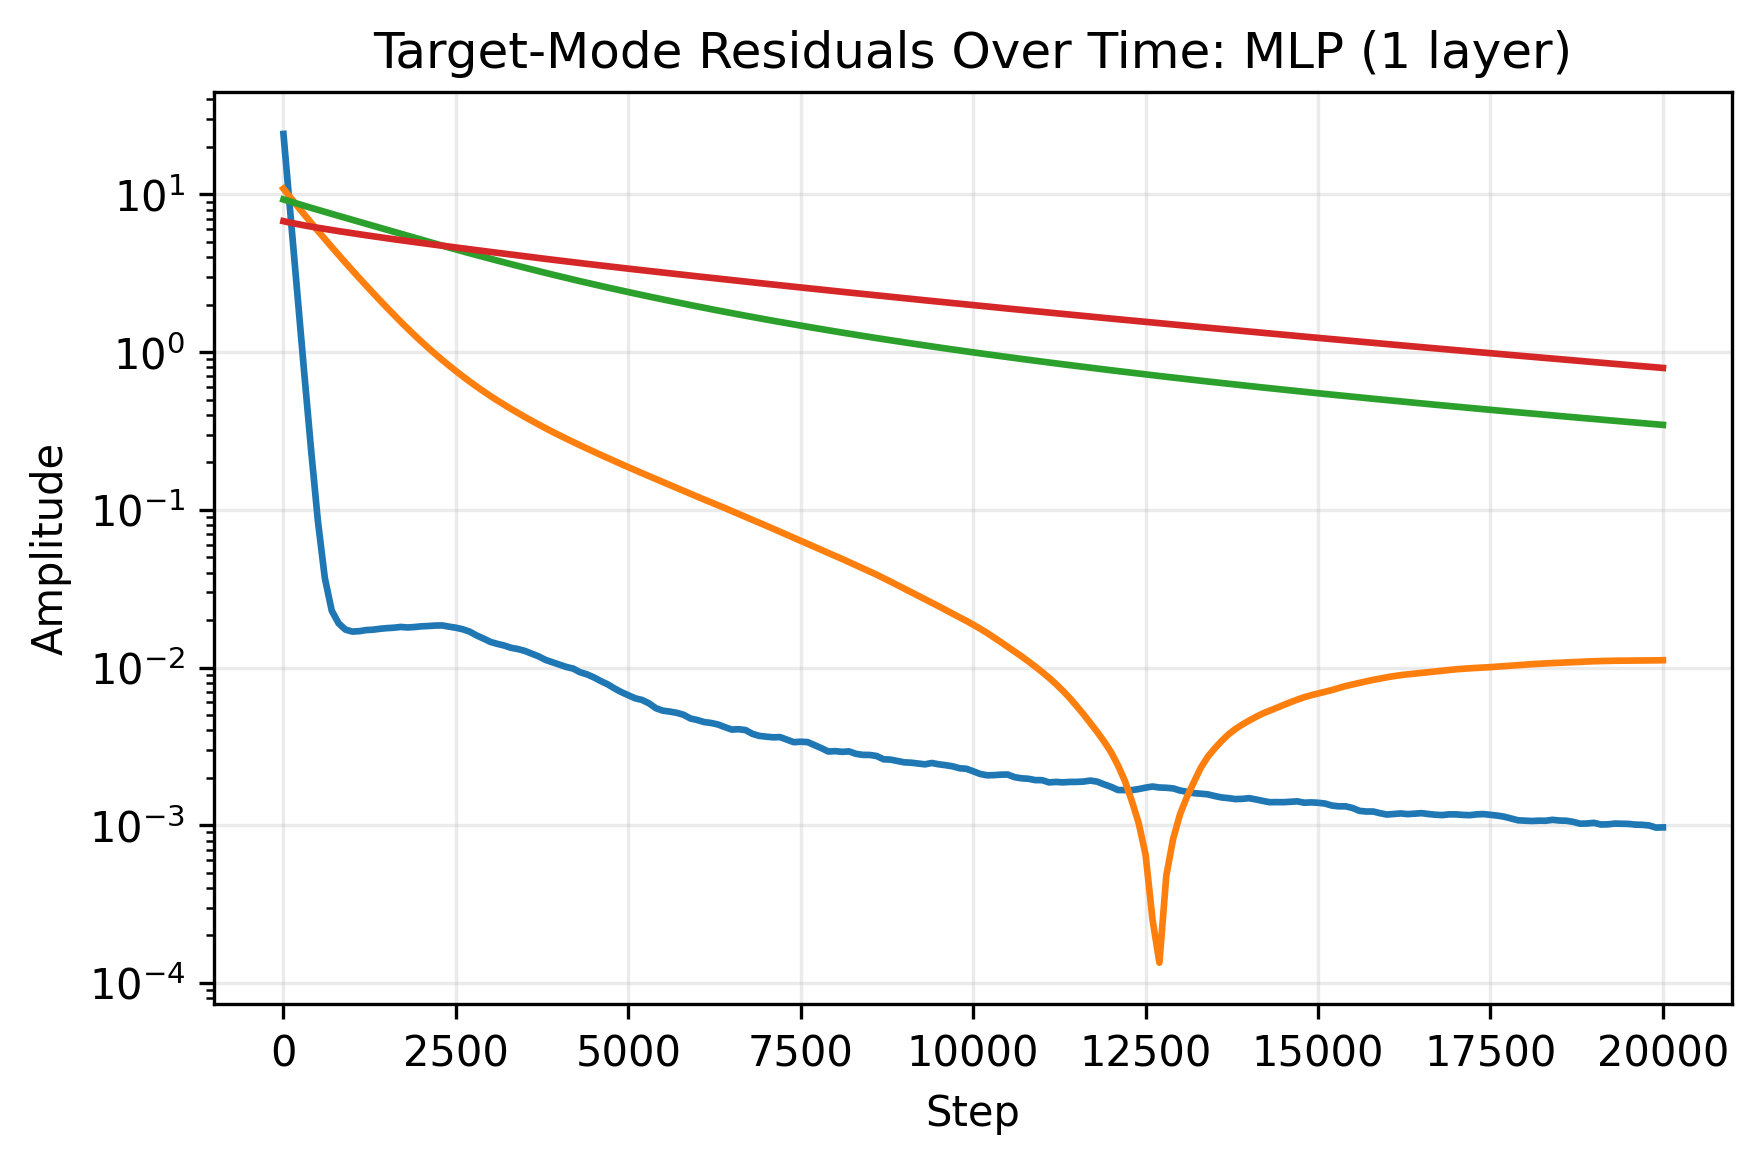
\includegraphics[width=\textwidth]{images/preliminary/mode_residuals_over_time_MLP_(1_layer).png}
		\caption{Single-hidden-layer MLP.}
		\label{fig:prelim-mlp-shallow}
	\end{subfigure}\hfill
	\begin{subfigure}[t]{0.33\textwidth}
		\centering
		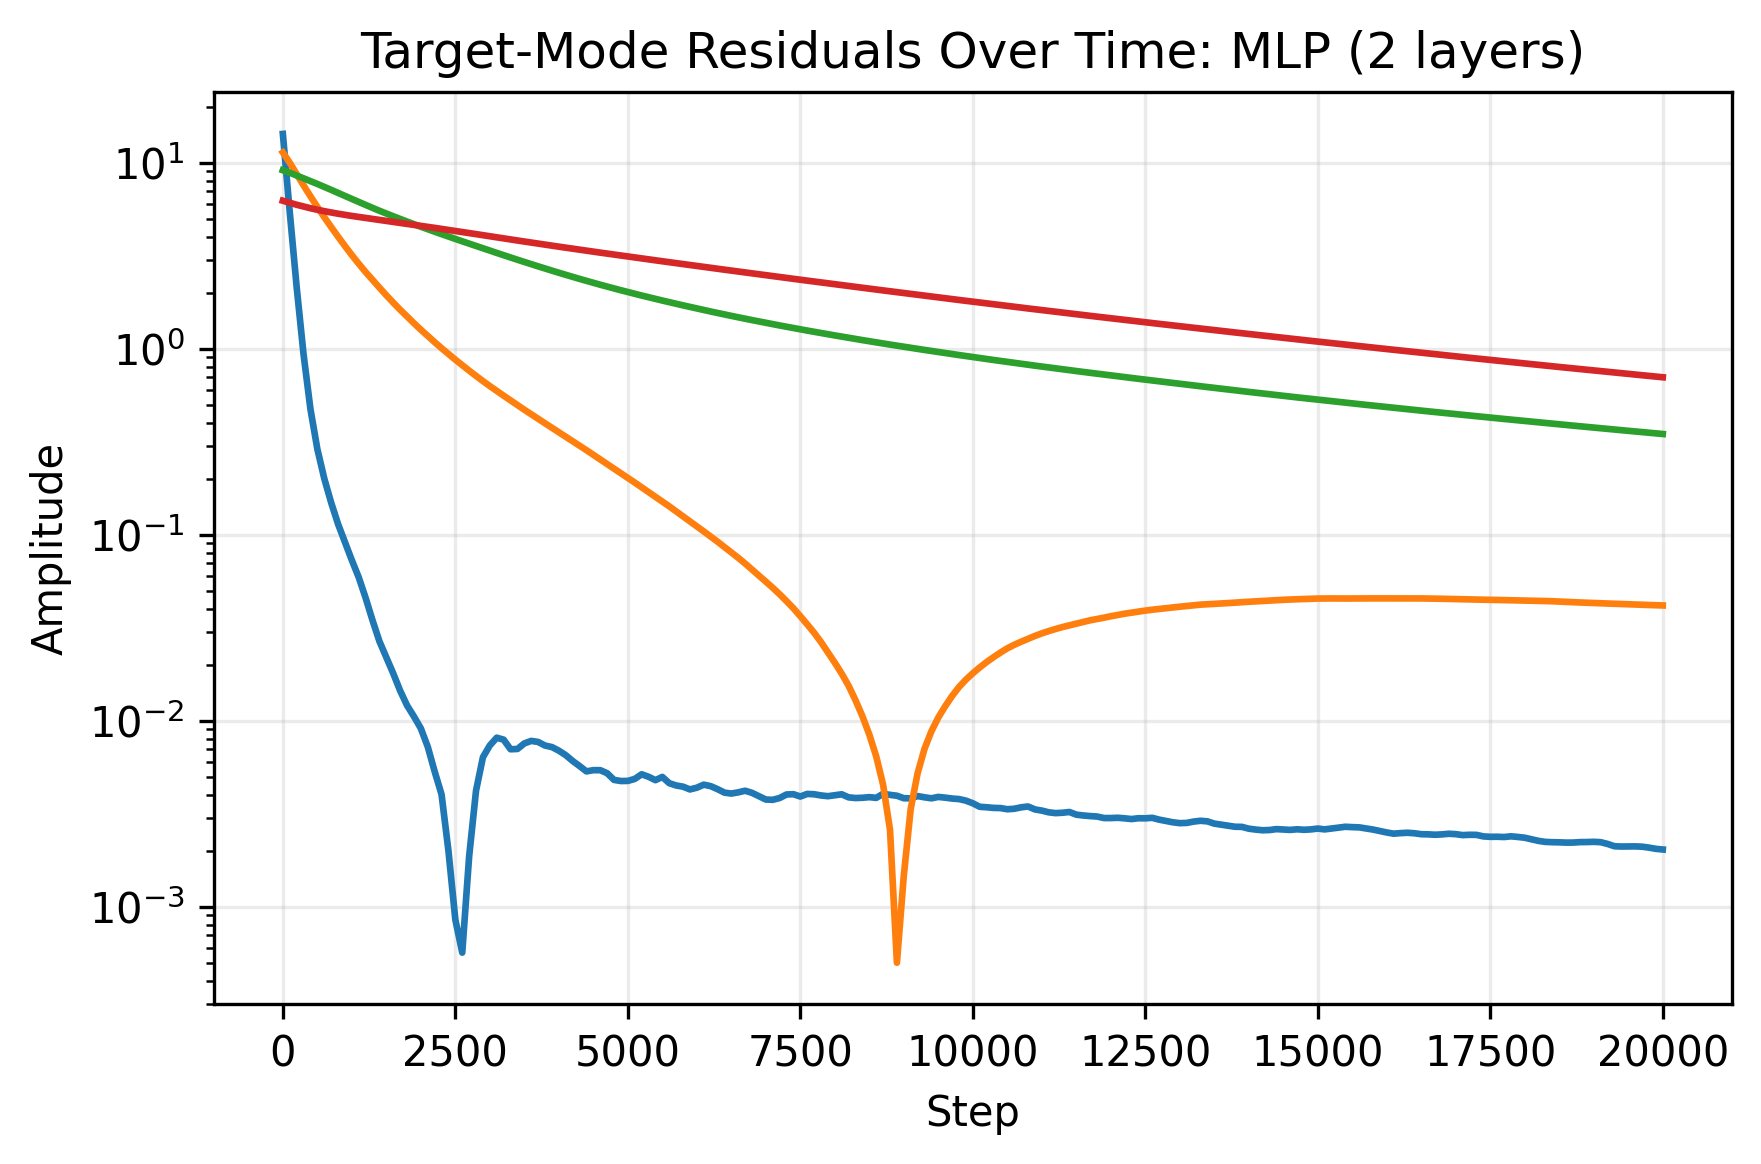
\includegraphics[width=\textwidth]{images/preliminary/mode_residuals_over_time_MLP_(2_layers).png}
		\caption{Two-layer MLP.}
		\label{fig:prelim-mlp-deep}
	\end{subfigure}\hfill
	\begin{subfigure}[t]{0.33\textwidth}
		\centering
		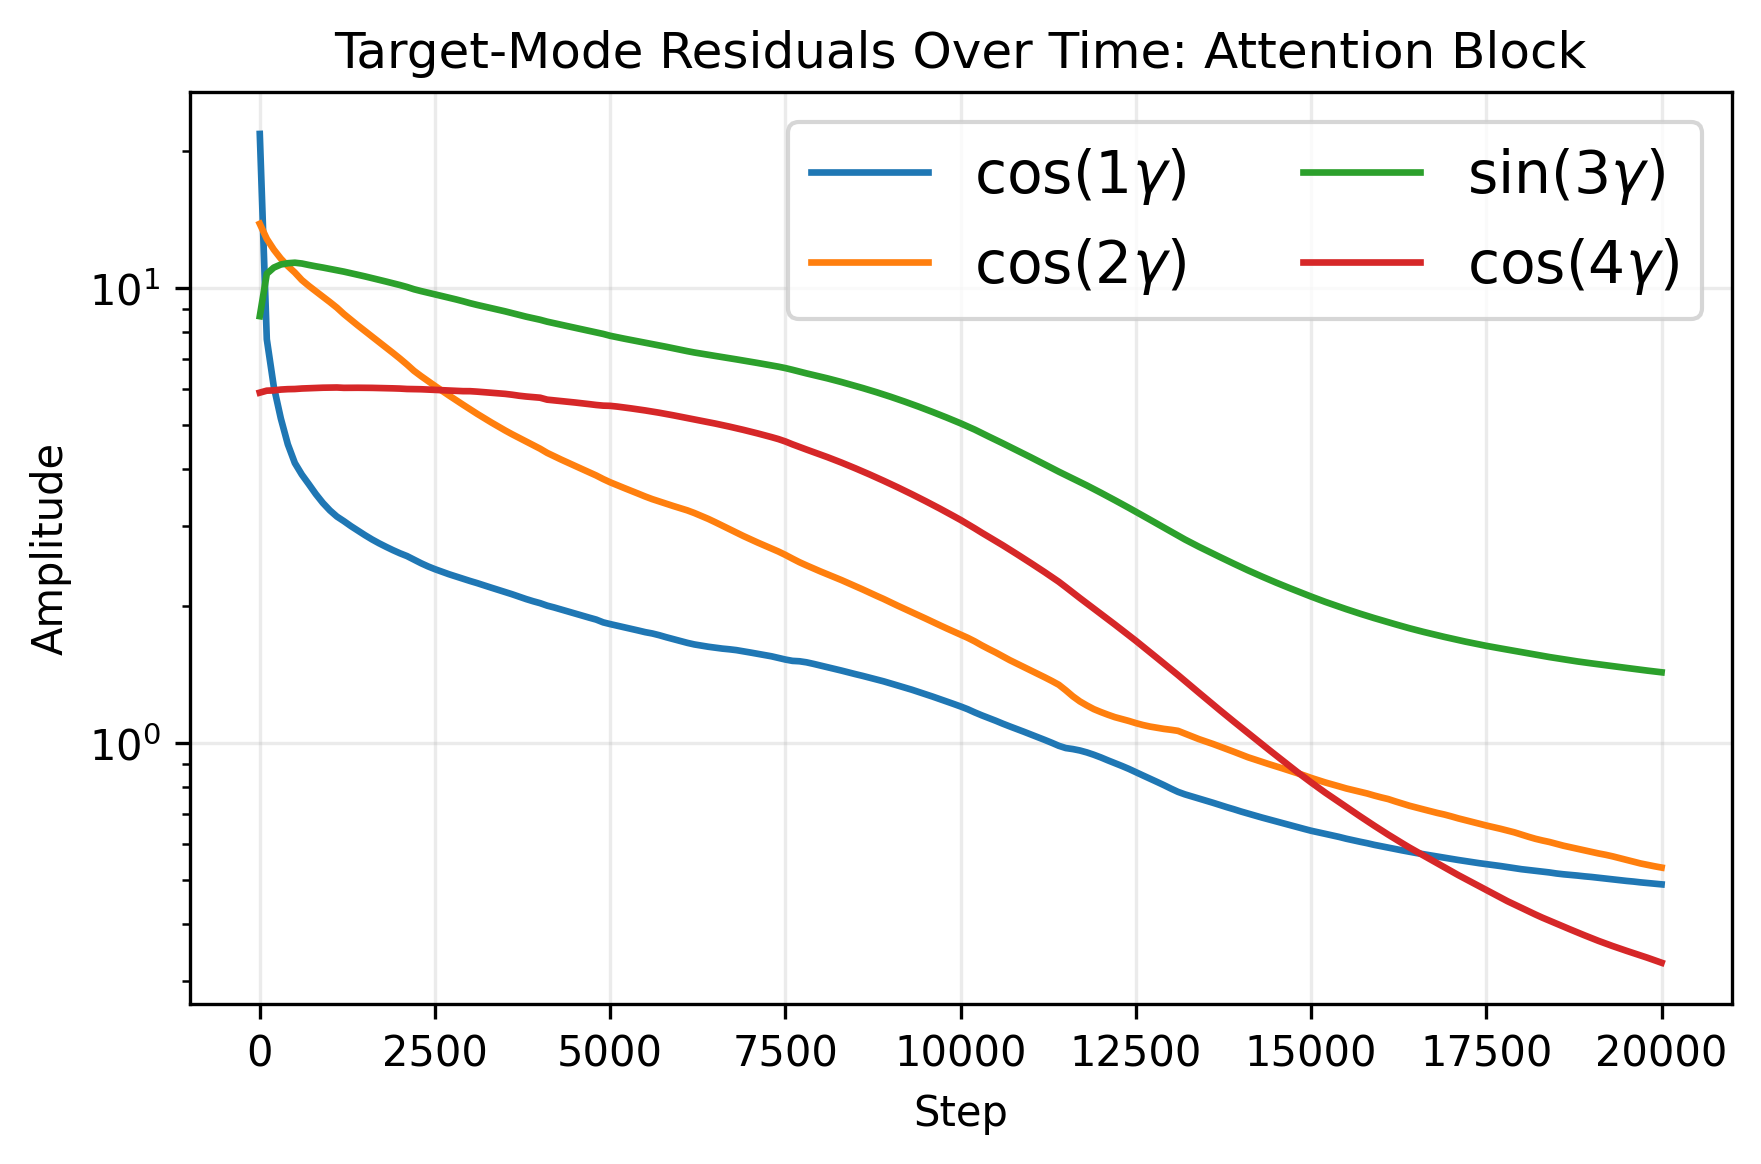
\includegraphics[width=\textwidth]{images/preliminary/mode_residuals_over_time_attention_block.png}
		\caption{Attention block.}
		\label{fig:prelim-attention}
	\end{subfigure}

	\caption{Preliminary experiments across architectures trained at finite width on
		finite data. Each panel shows the residual amplitude of four target modes,
		\(\cos\gamma\), \(\cos 2\gamma\), \(\sin 3\gamma\), and \(\cos 4\gamma\),
		against training step on a logarithmic scale.}
	\label{fig:preliminary-frequency-architectures}
\end{figure}

Figure~\ref{fig:preliminary-frequency-architectures} shows these experiments. In
every case the lowest-frequency mode \(\cos\gamma\) collapses first, within the
first few hundred steps, while the higher-frequency modes decay more slowly, so the
broad low-frequency-first ordering holds across all three architectures. The
ordering is not strict: in the MLPs \(\cos 2\gamma\) overtakes the higher modes and
its coefficient passes through zero, and in the attention block the modes are more
tangled and \(\cos 4\gamma\) eventually decays past the others. Frequency-dependent
learning is therefore not specific to the one-hidden-layer setting, but the precise
spectral picture depends on the operator induced by the architecture, the finite
sample, and the finite-width kernel. This is what motivates the controlled analysis
that follows, where the infinite-width reference operator is explicit and the
effects of finite sampling and finite width can be separated.

\begin{revblock}
	\section{Research gap}\label{sec:research-gap}

	The preceding discussion shows that spectral bias has a clean explanation in
	idealized fixed-kernel settings. In the infinite-width NTK regime, training is
	governed by a fixed operator whose spectrum determines the decay rates of the
	corresponding components of the residual
	\citep{jacot2018ntk,cao2020understandingspectralbiasdeep}. In symmetric
	settings, such as the circle or sphere with the uniform measure, this operator
	can be diagonalized by Fourier or harmonic modes, giving a precise version of
	the ``low frequencies first'' phenomenon
	\citep{basri2019convergence,basri2020frequencybiasneuralnetworks,
		bietti2019inductivebiasneuraltangent}.

	\citet{bowman2022spectralbiasoutsidetraining} prove bounds comparing the
	trajectory of a finite-width network trained on finitely many samples with the
	idealized NTK dynamics obtained at infinite width and infinite data. The
	comparison holds in \(L^2\) over the input distribution and up to a finite time
	horizon, so it describes the learned function away from the training samples as
	well. Their result shows that the network can inherit the bias of the NTK
	integral operator toward its leading eigenfunctions. However, their analysis is
	general as it does not focus on a setting where the eigenfunctions can be written
	explicitly as Fourier modes, nor does it separately track how finite sampling
	and finite width perturb those Fourier eigenspaces.

	This motivates studying a setting where the ideal operator is explicit enough
	that its perturbations can be inspected directly. The circle \(S^1\) with the
	uniform measure provides such a setting. The limiting NTK is a convolution
	operator, the Fourier modes are exact eigendirections, and the corresponding
	eigenvalues can be computed explicitly. This lets us separate the effects that
	are otherwise mixed together: the effect of replacing the continuum measure by
	a finite sample, the effect of replacing the infinite-width kernel by a
	finite-width random kernel, and the effect of allowing the tangent kernel to
	evolve during training.

	What is still missing is therefore a direct account of how the Fourier
	description on \(S^1\) changes under these perturbations.  One would expect the
	low-frequency Fourier structure to persist approximately under finite sampling
	and finite width. In other words, the perturbed eigenvalues should remain close
	to their continuum values, and the eigenspaces of the perturbed operator should
	remain close to the corresponding Fourier frequency subspaces. At the same
	time, these approximations should become more fragile when eigenvalues are
	small, when gaps between eigenvalues are narrow (e.g. in higher frequencies),
	or when the kernel evolves during training.

	\section{Research questions}

	This thesis studies spectral bias on \(S^1\) by comparing the residual dynamics induced by the
	continuum infinite-width NTK operator with those induced by its finite-sample and finite-
	width counterparts.

	Since the full operator acts on an infinite-dimensional function space, we make
	the comparisons on a finite Fourier subspace. For \(K > 0\), let
	\[
		\mathcal H_K
		:=
		\operatorname{span}
		\{1,\sqrt{2}\cos(k\theta),\sqrt{2}\sin(k\theta):1\le k\le K\}.
	\]
	This subspace contains the constant mode and the first \(K\) non-zero Fourier
	frequencies. Working on \(\mathcal H_K\) gives a controlled way to test how far
	the ideal Fourier-mode explanation of spectral bias survives at finite sample
	size and finite width.
\end{revblock}

\paragraph{Main research question.}
To what extent does the spectral decomposition of the continuum infinite-width
NTK operator on \(S^1\) persist on a fixed low-frequency Fourier subspace
\(\mathcal H_K\) under finite-sample and finite-width perturbations?

\paragraph{Subquestions.}
\begin{enumerate}
	\item[(RQ1)] \textbf{Finite-sample perturbation of the continuum operator.}
	      In the infinite-width regime, how does replacing the uniform measure
	      on \(S^1\) by \(n\) i.i.d.\ sampled points affect the action of the
	      continuum NTK operator on the fixed truncated Fourier subspace
	      \(\mathcal H_K\)?
	      More precisely, how close is the sampled operator to the diagonal
	      Fourier prediction on this subspace, and what are the consequences
	      for the associated residual dynamics?
	\item[(RQ2)] \textbf{Finite-width perturbation in the continuum setting.}
	      With the continuum measure on \(S^1\) kept fixed, how does finite
	      network width affect the tangent-kernel dynamics on the fixed truncated
	      Fourier subspace \(\mathcal H_K\), both at initialization and during
	      training?
	      More precisely, how close is the finite-width tangent kernel at
	      initialization to the infinite-width tangent kernel, and how does
	      the evolution of this tangent kernel during training change the decay of Fourier
	      modes, their alignment, and their effective learning rates?
\end{enumerate}

\section{Contributions}
\label{sec:contributions}

\begin{itemize}
	\item We derive the infinite-width reference model for the specific network
	      studied in this thesis. Closely related two-layer analyses often
	      simplify the NTK by training only the first-layer weights and biases
	      while keeping the output weights fixed
	      \citep{basri2019convergence,basri2020frequencybiasneuralnetworks}.
	      Here, we keep the output weights trainable and include their
	      contribution to the NTK. This gives an explicit kernel on \(S^1\),
	      explicit Fourier learning rates, and the baseline used in the rest of
	      the thesis.

	\item We study how this Fourier-frequency picture changes when the continuum
	      input distribution is replaced by finitely many sampled points. For a
	      fixed low-frequency subspace, we prove non-asymptotic bounds showing
	      that the sampled Fourier structure remains close to the idealized
	      continuum prediction when the sample size is large enough.

	\item We support the finite-sample analysis with numerical experiments. These
	      experiments compare the predicted frequency-wise learning rates with
	      the rates observed on sampled data, and show that the agreement improves
	      as the number of samples increases.

	\item We study the effect of finite network width when the tangent kernel is
	      frozen at initialization. On the same low-frequency subspace, we prove
	      that the finite-width operator concentrates around the infinite-width
	      prediction as width increases, and we verify this numerically using
	      eigenspace-alignment diagnostics.

	\item We empirically study the evolving finite-width tangent kernel during
	      training. We compare frozen and evolving dynamics across widths, and track
	      mode-wise residual decay, Fourier-subspace alignment, effective decay-rates,
	      and kernel drift. The experiments suggest that kernel evolution
	      helps at small width mainly by increasing low-frequency spectral
	      strength, even though it can move some eigenspaces away from the Fourier
	      reference. This advantage becomes smaller as width increases.
\end{itemize}

Together, these results show how the clean Fourier description from the
infinite-width model changes when we move to finite data and finite network
width. For finite sampling and frozen finite width, we give explicit
non-asymptotic bounds. For the evolving finite-width kernel during training, we
provide an empirical analysis showing how kernel evolution changes residual
decay, Fourier alignment, and spectral strength. Developing comparable theory
for this evolving-kernel regime remains the main open direction.

\chapter{Methodology}\label{cha:methodology}

This chapter defines the operators, projections, and diagnostics used throughout
the thesis, and states what each object measures and how it enters the
finite-sample and finite-width experiments. Detailed derivations are given in the
appendices.

\section{Mathematical setting}

\subsection{Domain and measure}

We identify the unit circle \(S^1\) with the angular domain \(\Omega=[0,2\pi)\), equipped
with the uniform probability measure
\begin{equation}
	d\mu(\varphi)=\frac{d\varphi}{2\pi}.
	\label{eq:method-uniform-measure}
\end{equation}
The embedding into \(\mathbb R^2\) is given by
\begin{equation}
	x(\varphi)=(\cos\varphi,\sin\varphi)\in S^1\subset\mathbb R^2.
	\label{eq:method-circle-embedding}
\end{equation}
This parametrization makes the rotational symmetry of the problem explicit and provides the
natural Fourier basis for \(L^2(\mu)\).

\subsection{Network model}

We consider a one-hidden-layer ReLU network in NTK parameterization. For inputs
\(x\in S^1\subset\mathbb{R}^2\),
\begin{equation}
	f_m(x;\theta)=\frac{1}{\sqrt m}\sum_{i=1}^m a_i \sigma(w_i^\top x+b_i),
	\label{eq:method-network-model}
\end{equation}
where \(\theta=\{(a_i,w_i,b_i)\}_{i=1}^m\), \(\sigma(t)=t_+=\max\{t,0\}\), and the parameters are
initialized according to
\begin{equation}
	a_i \sim \mathcal{N}(0,1),
	\qquad
	w_i \sim \mathcal{N}(0,I_2),
	\qquad
	b_i(0)=0,
	\label{eq:method-network-initialization}
\end{equation}
independently across \(i=1,\dots,m\). The bias parameters are initialized at zero but remain
trainable throughout.

\subsection{Least-squares loss and residual dynamics}
\label{subsec:least-squares-loss-and-residual-dynamics}

Let \(y\in L^2(\mu)\) be the target function, and write
\[
	f_t(\varphi):=f_m(x(\varphi);\theta(t))
\]
for the network output at training time \(t\). We consider the least-squares loss
\begin{equation}
	\mathcal{L}(\theta)
	=
	\frac{1}{2}\|f_m(\cdot;\theta)-y\|_{L^2(\mu)}^2
	=
	\frac{1}{2}\int_0^{2\pi}\bigl(f_m(\varphi;\theta)-y(\varphi)\bigr)^2\,d\mu(\varphi).
	\label{eq:method-loss-functional}
\end{equation}
We define the residual
\begin{equation}
	r_t(\varphi)=f_t(\varphi)-y(\varphi).
	\label{eq:method-residual-function}
\end{equation}

At finite width, the empirical neural tangent kernel at time \(t\) is
\begin{equation}
	\Theta_t^{(m)}(\varphi,\psi)
	=
	\bigl\langle \nabla_\theta f_m(\varphi;\theta(t)),
	\nabla_\theta f_m(\psi;\theta(t))\bigr\rangle,
	\label{eq:method-empirical-ntk}
\end{equation}
and the corresponding integral operator \(T_t^{(m)}:L^2(\mu)\to L^2(\mu)\) is
\begin{equation}
	(T_t^{(m)}f)(\varphi)
	=
	\int_0^{2\pi}\Theta_t^{(m)}(\varphi,\psi)f(\psi)\,d\mu(\psi).
	\label{eq:method-time-dependent-kernel-operator}
\end{equation}
Under gradient flow, the residual evolves according to
\begin{equation}
	\partial_t r_t=-T_t^{(m)}r_t.
	\label{eq:method-exact-residual-flow}
\end{equation}
Consequently, the loss evolves as
\begin{equation}
	\frac{d}{dt}\frac12\|r_t\|_{L^2(\mu)}^2
	=
	-\langle r_t,T_t^{(m)}r_t\rangle_{L^2(\mu)}.
	\label{eq:method-loss-decay-identity}
\end{equation}
Loss decay therefore depends not only on the eigenspaces of \(T_t^{(m)}\), but
also on how strongly the operator acts on the directions where the residual has
mass.

This equation contains both the frozen and evolving regimes. In the frozen regime,
\(T_t^{(m)}\) is replaced by its initial value
\begin{equation}
	T_0^{(m)}:=T_t^{(m)}\big|_{t=0},
	\label{eq:method-frozen-operator}
\end{equation}
whereas in the evolving regime the full time dependence of \(T_t^{(m)}\) is retained.

\section{Continuum reference model}

\subsection{Infinite-width tangent operator}

The first object studied in the thesis is the infinite-width limiting tangent operator
\begin{equation}
	T_\infty:=\lim_{m\to\infty} T_0^{(m)},
	\label{eq:method-infinite-width-operator}
\end{equation}
whose kernel is denoted by \(\Theta\). Under the initialization
\eqref{eq:method-network-initialization}, the limiting kernel exists and is deterministic.
The explicit formula for \(\Theta\) and the corresponding Fourier eigenvalues are stated in
Chapter~\ref{cha:results} and derived in Appendix~\ref{app:continuum-kernel}.

\subsection{Translation invariance and Fourier diagonalization}

Because the input distribution is uniform and the limiting kernel is rotation-invariant,
\(\Theta(\varphi,\psi)\) depends only on the angular difference. The limiting operator
therefore takes the convolution form
\begin{equation}
	(T_\infty f)(\varphi)
	=
	\int_0^{2\pi}\Theta(\varphi-\psi)f(\psi)\,d\mu(\psi),
	\label{eq:method-continuum-operator}
\end{equation}
and is diagonalized by the real Fourier basis of \(L^2(\mu)\). Its eigenvalues determine the
decay rates of the Fourier components of the residual in the ideal fixed-kernel continuum
model.

This continuum Fourier decomposition serves as the reference point for the finite-sample and
finite-width analyses below.

\subsection{Real Fourier basis and truncated subspaces}
\label{subsec:real-fourier-basis-truncates-subspaces}

We define the real Fourier basis of \(L^2(\mu)\) by
\begin{equation}
	\phi_0(\varphi)=1,
	\label{eq:method-fourier-basis-phi0}
\end{equation}
and, for each \(k\geq 1\),
\begin{equation}
	\phi_{k,c}(\varphi)=\sqrt{2}\cos(k\varphi),
	\qquad
	\phi_{k,s}(\varphi)=\sqrt{2}\sin(k\varphi).
	\label{eq:method-fourier-basis-modes}
\end{equation}
For a fixed cutoff \(K\geq 1\), we consider the truncated subspace
\begin{equation}
	\mathcal{H}_K=\operatorname{span}\{\phi_0,\phi_{k,c},\phi_{k,s}:1\leq k\leq K\},
	\label{eq:method-low-frequency-subspace}
\end{equation}
with dimension
\begin{equation}
	d=2K+1.
	\label{eq:method-block-dimension}
\end{equation}
Let
\begin{equation}
	P_K:L^2(\mu)\to \mathcal{H}_K
	\label{eq:method-projection-PK}
\end{equation}
denote the orthogonal projection onto $\mathcal H_K$.

The truncation to \(\mathcal{H}_K\) is used throughout the thesis to reduce the continuum problem to a
finite-dimensional low-frequency block that can be compared across the continuum, sampled,
frozen finite-width, and evolving finite-width settings.

\section{Finite-sample methodology}
\label{sec:finite-sample-methodology}

\subsection{Finite-sample question}

We first study the effect of replacing the measure \(\mu\) by finitely many sampled points. Let
\begin{equation}
	\varphi_1,\dots,\varphi_n \overset{\mathrm{iid}}{\sim} \mathrm{Unif}[0,2\pi).
	\label{eq:method-sampled-angles}
\end{equation}
The main question is whether the diagonal Fourier decomposition of the continuum operator
remains approximately valid after this replacement.

\subsection{Sampled objects}

To study the sampled operator on \(\mathcal{H}_K\), we introduce the feature matrix
\(\Phi\in\mathbb{R}^{n\times d}\),
\begin{equation}
	\Phi_{i,p}=\phi_p(\varphi_i),
	\qquad
	1\leq i\leq n,\quad 1\leq p\leq d,
	\label{eq:method-feature-matrix}
\end{equation}
and the normalized sampled kernel matrix \(A\) with
\begin{equation}
	A_{ij}=\frac{1}{n}\Theta(\varphi_i-\varphi_j).
	\label{eq:method-empirical-operator}
\end{equation}
From these we form the Gram matrix
\begin{equation}
	G=\frac{1}{n}\Phi^\top\Phi,
	\label{eq:method-gram-matrix}
\end{equation}
and the compressed operator matrix
\begin{equation}
	H=\frac{1}{n}\Phi^\top A\Phi.
	\label{eq:method-compressed-operator}
\end{equation}
We also introduce the diagonal matrix
\begin{equation}
	\Lambda^{(n)}=\operatorname{diag}(\lambda_p^{(n)}),
	\label{eq:method-finite-sample-eigenvalue-matrix}
\end{equation}
whose entries are the finite-sample corrected Fourier eigenvalues defined in
Chapter~\ref{cha:results}.

\subsection{Quantities to be controlled}
The finite-sample analysis controls how far three sampled quantities deviate from
the values they would take if the sampled Fourier structure were exact. Each is
written as the difference between the sampled quantity and its ideal value:
\begin{equation}
	\underbrace{G-I_d}_{\text{basis vs.\ orthonormal}},
	\qquad
	\underbrace{H-\Lambda^{(n)}}_{\text{operator vs.\ diagonal}},
	\qquad
	\underbrace{A\Phi-\Phi\Lambda^{(n)}}_{\text{modes vs.\ eigenvectors}}.
	\label{eq:method-finite-sample-objects}
\end{equation}
The first is small when the sampled Fourier basis is close to orthonormal, so its
Gram matrix \(G\) is close to the identity. The second is small when the sampled
operator restricted to \(\mathcal H_K\), represented by \(H\), is close to the
diagonal finite-sample prediction \(\Lambda^{(n)}\). The third is small when the
sampled Fourier modes are close to being eigenvectors of the sampled operator,
i.e.\ applying the operator \(A\) to the modes \(\Phi\) reproduces them scaled by
the predicted eigenvalues. Together these are the quantities needed to answer Q1.

\section{Fourier-block preconditioning methodology}
\label{sec:method-preconditioning}

The finite-sample analysis gives a diagonal reference for the sampled operator on
a fixed Fourier block. We use it to define a preconditioning experiment that tests
whether the predicted Fourier eigenvalues explain the observed rate separation
between retained Fourier modes.

Fix a retained Fourier block
\[
	\mathcal H_K
	=
	\operatorname{span}\{\phi_0,\phi_{1,c},\phi_{1,s},\dots,\phi_{K,c},\phi_{K,s}\},
\]
with dimension \(d=2K+1\). Let
\[
	\Phi\in\mathbb R^{n\times d}
\]
be the sampled Fourier feature matrix, and let \(A\in\mathbb R^{n\times n}\) be
the normalized sampled kernel operator. Recall that
\begin{equation}
	G=\frac1n\Phi^\top\Phi,
	\qquad
	H=\frac1n\Phi^\top A\Phi.
	\label{eq:method-preconditioning-GH}
\end{equation}
The matrix \(G\) is the sampled Fourier Gram matrix, while \(H\) records the
action of the sampled operator \(A\) on the retained Fourier basis.
When \(G\) is invertible, define
\begin{equation}
	C_n^{(K)}
	:=
	G^{-1}H.
	\label{eq:method-sampled-coefficient-operator}
\end{equation}
This matrix describes what the sampled operator \(A\) does to the Fourier
coefficients on the retained block. Indeed, if \(u=\Phi z\), then \(z\) is the
coefficient vector of \(u\) in the sampled Fourier basis. After applying \(A\),
the least-squares coefficients of \(Au\) in the same sampled Fourier basis are
\begin{equation}
	G^{-1}\frac1n\Phi^\top (Au)
	=
	G^{-1}\frac1n\Phi^\top A\Phi z
	=
	C_n^{(K)}z.
	\label{eq:method-sampled-coefficient-action}
\end{equation}
Thus \(C_n^{(K)}\) is the object that should be compared with the diagonal
finite-sample prediction
\begin{equation}
	\Lambda^{(n)}
	=
	\operatorname{diag}(\lambda_p^{(n)}).
	\label{eq:method-preconditioning-lambda-n}
\end{equation}
The finite-sample theory predicts that, on the retained block,
\begin{equation}
	C_n^{(K)}
	\approx
	\Lambda^{(n)}.
	\label{eq:method-coefficient-operator-approx}
\end{equation}
This means that, on the retained Fourier block, the sampled operator is expected
to act mainly by rescaling each Fourier coefficient by its predicted eigenvalue,
with only small mixing between different retained Fourier modes.

We now define two preconditioners from this comparison. First note that, for any
sampled vector \(v\in\mathbb R^n\),
\[
	G^{-1}\frac1n\Phi^\top v
\]
gives the least-squares Fourier coefficients of the projection of \(v\) onto
the sampled span of the retained modes. Thus, to correct the action of \(A\) on
the retained block, we first apply \(A\), then project back onto the retained
Fourier span, and finally rescale the resulting Fourier coefficients.

The theory preconditioner uses the diagonal prediction \(\Lambda^{(n)}\):
\begin{equation}
	P_{\mathrm{th}}
	:=
	\frac1n
	\Phi
	\bigl(\Lambda^{(n)}\bigr)^{-1}
	G^{-1}
	\Phi^\top .
	\label{eq:method-theory-preconditioner}
\end{equation}
This operator projects a sampled vector onto the retained Fourier span and
rescales each retained Fourier coefficient by the inverse predicted eigenvalue.
It uses the analytic prediction \(\Lambda^{(n)}\), and therefore does not use
the observed matrix \(C_n^{(K)}\).

The empirical preconditioner uses the observed retained block:
\begin{equation}
	P_{\mathrm{emp}}
	:=
	\frac1n
	\Phi
	\bigl(C_n^{(K)}\bigr)^{-1}
	G^{-1}
	\Phi^\top .
	\label{eq:method-empirical-preconditioner}
\end{equation}
This operator uses the actual sampled matrix \(C_n^{(K)}\). It therefore
corrects both the diagonal scaling and the mixing between retained Fourier modes
that is present for the particular sampled points.

We compare three sampled dynamics:
\begin{equation}
	B_{\mathrm{base}}:=A,
	\qquad
	B_{\mathrm{th}}:=P_{\mathrm{th}}A,
	\qquad
	B_{\mathrm{emp}}:=P_{\mathrm{emp}}A.
	\label{eq:method-preconditioned-operators}
\end{equation}
The baseline \(B_{\mathrm{base}}\) is the original sampled kernel operator. The
operators \(B_{\mathrm{th}}\) and \(B_{\mathrm{emp}}\) apply the sampled kernel
operator and then correct its action through the retained Fourier block.

For sampled predictions \(f_t\in\mathbb R^n\), targets \(y\in\mathbb R^n\), and
residuals
\[
	r_t=f_t-y,
\]
we compare the gradient-flow dynamics
\begin{equation}
	\frac{d r_t}{dt}
	=
	- B r_t,
	\label{eq:method-sampled-operator-flow}
\end{equation}
with
\[
	B\in\{B_{\mathrm{base}},B_{\mathrm{th}},B_{\mathrm{emp}}\}.
\]

The effect is easiest to see on a vector \(u=\Phi z\) in the retained Fourier
span. Applying \(A\) and projecting back to the retained block gives the
coefficient vector \(C_n^{(K)}z\). Therefore
\begin{align}
	B_{\mathrm{th}}\Phi z
	 & =
	\Phi
	\bigl(\Lambda^{(n)}\bigr)^{-1}
	C_n^{(K)}z,
	\label{eq:method-theory-preconditioned-block-action}
\end{align}
while
\begin{align}
	B_{\mathrm{emp}}\Phi z
	 & =
	\Phi
	\bigl(C_n^{(K)}\bigr)^{-1}
	C_n^{(K)}z
	=
	\Phi z.
	\label{eq:method-empirical-preconditioned-block-action}
\end{align}
Thus on the retained block the empirical preconditioner reduces the action to the
identity: every retained Fourier mode is driven at the same rate, so the
frequency-dependent rate separation is removed, provided \(C_n^{(K)}\) is
invertible. The theory preconditioner achieves this only insofar as the observed
block \(C_n^{(K)}\) is close to the diagonal prediction \(\Lambda^{(n)}\); from
\eqref{eq:method-theory-preconditioned-block-action}, it leaves the residual
factor \((\Lambda^{(n)})^{-1}C_n^{(K)}\), which equals the identity exactly when
\(C_n^{(K)}=\Lambda^{(n)}\).

In the numerical experiments, ill-conditioned inverses are replaced by small
ridge-regularized inverses when needed, for example \((\Lambda^{(n)}+\tau I)^{-1}\)
or \((C_n^{(K)}+\tau I)^{-1}\) with \(\tau>0\). If \(B_{\mathrm{th}}\) and
\(B_{\mathrm{emp}}\) behave similarly, the predicted Fourier eigenvalues explain
most of the rate differences on the retained block; if \(B_{\mathrm{emp}}\) is
noticeably better, the sampled points introduce mixing between retained Fourier
modes that the diagonal prediction does not capture.

\section{Finite-width frozen-kernel methodology}

\subsection{Finite-width question}

We next remove sampling randomness and return to the continuum input space \(S^1\), but keep
the network width finite. The question is then whether the low-frequency block of the frozen
finite-width tangent operator remains close to the continuum Fourier block predicted by the
infinite-width theory.

\subsection{One-neuron tangent features and operators}

For each neuron \(r\), define its tangent feature at initialization by
\begin{equation}
	\psi_r(\varphi)
	=
	\nabla_{(a_r,w_r,b_r)}
	\bigl(a_r\sigma(w_r^\top x(\varphi)+b_r)\bigr).
	\label{eq:method-one-neuron-tangent-feature}
\end{equation}
The corresponding one-neuron kernel contribution is
\begin{equation}
	\Theta^{(r)}(\varphi,\psi)
	=
	\psi_r(\varphi)^\top \psi_r(\psi),
	\label{eq:method-one-neuron-kernel}
\end{equation}
and the associated one-neuron operator is
\begin{equation}
	(T^{(r)}f)(\varphi)
	=
	\int_0^{2\pi}\Theta^{(r)}(\varphi,\psi)f(\psi)\,d\mu(\psi).
	\label{eq:method-one-neuron-operator}
\end{equation}
At initialization, the frozen finite-width tangent operator is the average
\begin{equation}
	T_0^{(m)}=\frac1m\sum_{r=1}^m T^{(r)}.
	\label{eq:method-finite-width-frozen-average}
\end{equation}

\subsection{Projected frozen operator}

Let \( P_K:L^2(\mu)\to \mathcal H_K \)
denote the orthogonal projection onto the truncated Fourier subspace
\(\mathcal H_K\). The low-frequency block of the frozen finite-width operator is
\begin{equation}
	B_m^{(K)}:=P_KT_0^{(m)}P_K.
	\label{eq:method-finite-width-block}
\end{equation}
The corresponding continuum reference block is
\begin{equation}
	\Lambda_K:=P_KT_\infty P_K
	=
	\operatorname{diag}(\lambda_0,\lambda_1,\lambda_1,\dots,\lambda_K,\lambda_K).
	\label{eq:method-continuum-fourier-block}
\end{equation}
The finite-width frozen analysis asks whether \(B_m^{(K)}\) remains close to \(\Lambda_K\)
with high probability as \(m\) increases.

\subsection{Matrix representation of the frozen block}

Using the ordered basis
\[
	(\phi_0,\phi_{1,c},\phi_{1,s},\dots,\phi_{K,c},\phi_{K,s}),
\]
the projected operator \(B_m^{(K)}\) is represented by the matrix with entries
\begin{equation}
	(B_m^{(K)})_{pq}
	=
	\langle \phi_p,T_0^{(m)}\phi_q\rangle_{L^2(\mu)}.
	\label{eq:method-finite-width-block-entry}
\end{equation}
Equivalently,
\begin{equation}
	(B_m^{(K)})_{pq}
	=
	\frac1m\sum_{r=1}^m \xi_{r,pq},
	\qquad
	\xi_{r,pq}:=\langle \phi_p,T^{(r)}\phi_q\rangle,
	\label{eq:method-finite-width-entry-average}
\end{equation}
so that \(B_m^{(K)}\) is an empirical average of \(m\) i.i.d.\ one-neuron
matrices. Because the entries are averages of independent terms, they concentrate
around their mean as \(m\) grows, which is what the finite-width frozen
concentration result in the next chapter exploits.

\subsection{Fourier-plane alignment diagnostics}
\label{subsec:method-projector-error}

The continuum operator is diagonal in the Fourier basis. For each frequency
\(k\ge 1\), the cosine and sine modes have the same continuum eigenvalue
\(\lambda_k\). Because \(\phi_{k,c}\) and \(\phi_{k,s}\) share the eigenvalue
\(\lambda_k\), the continuum operator does not single out either one; only the
plane they span is determined. The object to compare against is therefore this
two-dimensional frequency subspace,
\[
	\mathcal F_k
	:=
	\operatorname{span}\{\phi_{k,c},\phi_{k,s}\},
	\qquad k\ge 1,
\]
For the constant mode, we set
\[
	\mathcal F_0:=\operatorname{span}\{\phi_0\}.
\]
Thus, the dimensionality \(d_0=1\) and \(d_k=2\) for \(k\ge 1\).

We use subspace-alignment diagnostics to compare these reference Fourier
subspaces with matched eigenspaces of the finite-width tangent operator. In the
frozen case this operator is \(T_0^{(m)}\). In the evolving case it is the
time-dependent operator \(T_t^{(m)}\).

The operator is defined on the continuum \(S^1\), but it cannot be eigen-decomposed
in closed form at finite width, so for the numerical diagnostics we discretise it
onto a uniform grid of \(N\) points,
\[
	\theta_j=\frac{2\pi j}{N},\qquad j=0,\dots,N-1,
\]
and carry out the eigendecomposition and subspace comparisons on this grid.

All vectors and matrices in this diagnostic are therefore finite-dimensional
representations of continuum functions on this grid.

Let \(U_k\in\mathbb R^{N\times d_k}\) be an orthonormal basis for the grid
representation of \(\mathcal F_k\), and define the corresponding orthogonal
projector
\begin{equation}
	P_k := U_kU_k^\top .
	\label{eq:method-fourier-projector}
\end{equation}

At each training time \(t\), we eigendecompose the grid representation of the
tangent operator, an \(N\times N\) symmetric matrix, and write its orthonormal
eigenvectors as \(v_1(t),\dots,v_N(t)\). For each eigenvector \(v_j(t)\), the
quantity
\[
	\|U_k^\top v_j(t)\|_2^2 \in [0,1]
\]
is the squared length of its projection onto \(\mathcal F_k\): it is \(1\) when
\(v_j(t)\) lies entirely in \(\mathcal F_k\) and \(0\) when it is orthogonal to
it. We build the matched empirical subspace \(\widehat{\mathcal F}_k(t)\) by taking
the \(d_k\) eigenvectors with the largest such values, the ones lying closest to
\(\mathcal F_k\). If \(\widehat U_k(t)\in\mathbb R^{N\times d_k}\) is an
orthonormal basis of \(\widehat{\mathcal F}_k(t)\), define
\begin{equation}
	\widehat P_k(t)
	:=
	\widehat U_k(t)\widehat U_k(t)^\top .
	\label{eq:method-empirical-projector}
\end{equation}

The projection error is
\begin{equation}
	\varepsilon_{k,F}^{(m)}(t)
	:=
	\|\widehat P_k(t)-P_k\|_F .
	\label{eq:method-projector-errors}
\end{equation}
The projectors \(P_k\) and \(\widehat P_k(t)\) depend only on the subspaces, not
on the bases chosen for them, so this distance is invariant to sign changes of
eigenvectors and to rotations of the cosine-sine basis inside a two-dimensional
Fourier plane, neither of which should count as a mismatch. It therefore measures
the geometric distance between the matched eigenspace and the reference Fourier
subspace, and \eqref{eq:method-projector-angle-identity} below expresses it
through the principal angles. For the frozen operator, we write
\[
	\varepsilon_{k,F}^{(m)}:=\varepsilon_{k,F}^{(m)}(0).
\]

We also report principal angles between
\(\widehat{\mathcal F}_k(t)\) and \(\mathcal F_k\). Principal angles are a
standard way to compare finite-dimensional subspaces
\citep{bjorck1973numerical}. If \(U_k\) and \(\widehat U_k(t)\) are orthonormal
bases for the two subspaces, then the cosines of the principal angles are the
singular values of \(U_k^\top \widehat U_k(t)\). We define
\[
	0\le \theta_{k,1}(t)\le \cdots \le \theta_{k,d_k}(t)\le \frac{\pi}{2}
\]
by
\begin{equation}
	\cos\theta_{k,i}(t)
	=
	s_i(U_k^\top \widehat U_k(t)),
	\qquad i=1,\dots,d_k,
	\label{eq:method-principal-angles}
\end{equation}
where \(s_i(\cdot)\) is the \(i\)-th largest singular value, so the cosines of the
principal angles are the singular values of \(U_k^\top\widehat U_k(t)\) ordered
from largest to smallest.

For \(k=0\), there is one principal angle because both spaces are
one-dimensional. For \(k\ge 1\), there are two principal angles because both
spaces are two-dimensional. The first angle measures the best aligned direction
between the two planes. The second angle measures the remaining independent
direction. Both angles must be small for the full Fourier plane to be well
aligned with the matched empirical eigenspace.

For the evolving-kernel experiments, we also summarize the principal angles by
the subspace cosine similarity
\begin{equation}
	s_k^{\mathrm{cos}}(t)
	:=
	\left(
	\frac{1}{d_k}
	\sum_{i=1}^{d_k}\cos^2\theta_{k,i}(t)
	\right)^{1/2}.
	\label{eq:method-subspace-cosine-similarity}
\end{equation}
This quantity is the root-mean-square of the cosines of the principal angles.
We use this aggregation to summarize one-dimensional and two-dimensional Fourier
subspaces with a single score per frequency. The score lies between \(0\) and
\(1\), with larger values indicating better alignment. It equals \(1\) exactly
when the matched empirical subspace is the same as the reference Fourier
subspace.

The projection distance and the principal angles are related by the standard
projector identity \citep{bjorck1973numerical}
\begin{equation}
	\|\widehat P_k(t)-P_k\|_F^2
	=
	2\sum_{i=1}^{d_k}\sin^2\theta_{k,i}(t).
	\label{eq:method-projector-angle-identity}
\end{equation}
Thus the projection error gives one scalar measure of subspace mismatch, while
the principal angles and subspace cosine similarity give more detailed views of
the same alignment.

\section{Finite-width evolving-kernel methodology}
\label{sec:finite-width-evolving-kernel-methodology}
\subsection{Projected evolving operator}

To study the actual training dynamics, we retain the time dependence of the
empirical tangent operator \(T_t^{(m)}\). Its block on the same retained
subspace \(\mathcal H_K\), the frequencies up to \(K\) used throughout, is
\begin{equation}
	C_t^{(K)}:=P_KT_t^{(m)}P_K.
	\label{eq:method-evolving-block}
\end{equation}

In the ordered Fourier basis of \(\mathcal H_K\), this block has entries
\begin{equation}
	(C_t^{(K)})_{pq}
	=
	\langle \phi_p,T_t^{(m)}\phi_q\rangle_{L^2(\mu)}.
	\label{eq:method-evolving-block-entry}
\end{equation}
At initialization,
\[
	C_0^{(K)}=B_m^{(K)}.
\]
If \(b_t=(I-P_K)r_t\) is the residual component outside the retained Fourier
block, then \(T_t^{(m)}b_t\) need not remain outside that block. Its projection
back into \(\mathcal H_K\) is
\begin{equation}
	L_t^{(K)}b_t
	=
	P_KT_t^{(m)}(I-P_K)r_t.
\end{equation}
We therefore define
\begin{equation}
	L_t^{(K)}:=P_KT_t^{(m)}(I-P_K).
	\label{eq:method-leakage-operator}
\end{equation}
This operator represents high-to-low frequency coupling. It measures how
residual components outside the retained block can influence the evolution of
the retained Fourier coefficients after the tangent operator is applied.

\subsection{Projected residual dynamics}

Let
\begin{equation}
	a_t:=P_Kr_t,
	\qquad
	b_t:=(I-P_K)r_t.
	\label{eq:method-low-high-residual-split}
\end{equation}
Projecting the exact residual equation \eqref{eq:method-exact-residual-flow} gives
\begin{equation}
	\partial_t a_t
	=
	-C_t^{(K)}a_t
	-
	L_t^{(K)}b_t.
	\label{eq:method-projected-residual-flow}
\end{equation}
Thus the low-frequency dynamics is driven by two terms: the operator restricted
to \(\mathcal H_K\), and the contribution from residual components outside
\(\mathcal H_K\).

\subsection{Frozen versus evolving comparison}

The frozen and evolving regimes differ only through the time dependence of the operator. In
the frozen regime,
\[
	C_t^{(K)}\equiv C_0^{(K)}=B_m^{(K)},
\]
whereas in the evolving regime the operator changes during training. This motivates the
decomposition
\begin{equation}
	C_t^{(K)}
	=
	\Lambda_K
	+
	\bigl(C_0^{(K)}-\Lambda_K\bigr)
	+
	\bigl(C_t^{(K)}-C_0^{(K)}\bigr),
	\label{eq:method-operator-decomposition}
\end{equation}
which separates three effects:

\begin{enumerate}
	\item the ideal infinite-width Fourier block \(\Lambda_K\),
	\item the finite-width initialization error \(C_0^{(K)}-\Lambda_K\),
	\item the time-dependent kernel drift \(C_t^{(K)}-C_0^{(K)}\).
\end{enumerate}

The frozen-kernel theory studies the second term. The evolving-kernel
experiments study the third term empirically: how much the tangent operator
changes during training, and how these changes affect the Fourier-block
structure.

\subsection{Frequency-wise spectral strength}
\label{subsec:method-spectral-strength}

The subspace-alignment diagnostics measure whether the eigenspaces of the
finite-width tangent operator remain close to the Fourier subspaces. They do
not, however, measure how strongly the operator acts on those subspaces.
For the residual dynamics, this distinction matters because the loss decay is
controlled by \(\langle r_t,T_t^{(m)}r_t\rangle_{L^2(\mu)}\), as shown in
\eqref{eq:method-loss-decay-identity}. Thus the loss decay depends not only on
the orientation of the eigenspaces, but also on the magnitude of the operator in
directions where the residual has mass.
For each Fourier frequency subspace \(\mathcal F_k\), with orthogonal projector
\(P_k\) and dimension \(d_k\), we define the average spectral strength
\begin{equation}
	\mu_{\mathcal F_k}(t)
	:=
	\frac{1}{d_k}
	\operatorname{tr}\!\left(P_k T_t^{(m)} P_k\right).
	\label{eq:method-frequency-spectral-strength}
\end{equation}
Equivalently, if \(U_k\) is an orthonormal basis for \(\mathcal F_k\), then
\begin{equation}
	\mu_{\mathcal F_k}(t)
	=
	\frac{1}{d_k}
	\operatorname{tr}\!\left(U_k^\top T_t^{(m)} U_k\right).
	\label{eq:method-frequency-spectral-strength-basis}
\end{equation}
This quantity is basis-invariant within \(\mathcal F_k\). If \(\mathcal F_k\)
is an invariant eigenspace of the operator, then
\(\mu_{\mathcal F_k}(t)\) equals the corresponding eigenvalue. In general, it
should instead be interpreted as the average kernel strength inside that
Fourier block.

For \(k\le K\), the same quantity can be read directly from the low-frequency
block \(C_t^{(K)}\). It is the average trace of the diagonal block corresponding
to \(\mathcal F_k\):
\begin{equation}
	\mu_{\mathcal F_k}(t)
	=
	\frac{1}{d_k}
	\operatorname{tr}\!\left((C_t^{(K)})_{\mathcal F_k,\mathcal F_k}\right).
	\label{eq:method-frequency-spectral-strength-block}
\end{equation}

We also use the cumulative low-frequency strength
\begin{equation}
	\mu_{\le K}(t)
	:=
	\frac{1}{2K+1}
	\operatorname{tr}\!\left(P_KT_t^{(m)}P_K\right)
	=
	\frac{1}{2K+1}
	\sum_{k=0}^K d_k\,\mu_{\mathcal F_k}(t).
	\label{eq:method-cumulative-spectral-strength}
\end{equation}
This summarizes the average tangent-kernel strength over the retained
low-frequency block.

\section{Summary of the methodology}

The methodology consists of three comparisons.

First, the continuum infinite-width operator \(T_\infty\) gives the ideal
Fourier-diagonal reference model on \(S^1\). In this model, the Fourier modes
are exact eigenfunctions and the eigenvalues determine the residual decay rates.

Second, the finite-sample analysis studies what changes when the continuum
measure is replaced by finitely many sampled points. The main objects are the
sampled Fourier Gram matrix \(G\), the matrix \(H\) describing the action of
the sampled operator on the retained Fourier basis, and the difference
\(A\Phi-\Phi\Lambda^{(n)}\) between the sampled operator action and the
diagonal Fourier prediction. These objects are used to answer Q1. The rate
separation between modes comes from the spread of eigenvalues, so rescaling
each mode by its predicted eigenvalue should cancel it; the preconditioning
experiment uses this to test how much of the separation the eigenvalues
explain.

Third, the finite-width analysis studies what changes when the infinite-width
operator is replaced by the tangent operator of a finite-width network. The
frozen analysis focuses on \(B_m^{(K)}=P_KT_0^{(m)}P_K\), the low-frequency block
of the tangent operator at initialization. The evolving analysis tracks the
time-dependent block \(C_t^{(K)}=P_KT_t^{(m)}P_K\) and the high-to-low coupling
\(L_t^{(K)}=P_KT_t^{(m)}(I-P_K)\).

For the evolving experiments, we use two complementary kinds of diagnostics.
Projection error, principal angles, and subspace cosine similarity measure
whether the eigenspaces of the tangent operator remain close to the Fourier
subspaces.
Frequency-wise spectral strength measures how strongly the tangent operator
acts on each Fourier block. Together, these diagnostics separate changes in
Fourier geometry from changes in the magnitude of the kernel on the retained
frequency blocks.

\chapter{Results}
\label{cha:results}

\section{Continuum kernel on \(S^1\)}

We first state the explicit form of the limiting neural tangent kernel on the circle and the
corresponding Fourier eigenvalues of the integral operator \(T\) introduced in
Chapter~\ref{cha:methodology}. The calculation uses the standard infinite-width NTK
description of \citet{jacot2018ntk}, together with the
arc-cosine formulas for ReLU Gaussian averages \citep{cho2009kernel}. Related spectral
calculations for ReLU NTKs on the sphere appear in
\citet{basri2019convergence,bietti2019inductivebiasneuraltangent,cao2020understandingspectralbiasdeep}. The derivation in the
assumptions used here is given in Appendix~\ref{app:continuum-kernel}.

\begin{proposition}[Limiting NTK on \(S^1\)]
	\label{prop:results-continuum-ntk}
	Consider the finite-width network \(f_m\) and initialization from
	\eqref{eq:method-network-model}--\eqref{eq:method-network-initialization}.
	For \(x(\varphi)=(\cos\varphi,\sin\varphi)\), define the finite-width NTK at
	initialization by
	\[
		\Theta_m(\varphi,\psi)
		=
		\left\langle
		\nabla_\theta f_m(x(\varphi);\theta_0),
		\nabla_\theta f_m(x(\psi);\theta_0)
		\right\rangle .
	\]
	The limiting NTK is the deterministic kernel
	\[
		\Theta(\varphi,\psi)
		=
		\lim_{m\to\infty}\Theta_m(\varphi,\psi),
	\]
	where the limit is taken pointwise over the random initialization.

	If \(\delta=d(\varphi,\psi)\in[0,\pi]\) denotes the angular distance
	between \(x(\varphi)\) and \(x(\psi)\), then \(\Theta(\varphi,\psi)\) depends
	only on \(\delta\) and is given by
	\begin{equation}
		\Theta(\delta)
		=
		\frac{1}{2\pi}
		\Bigl(
		\sin\delta + 2(\pi-\delta)\cos\delta + (\pi-\delta)
		\Bigr).
		\label{eq:results-continuum-ntk}
	\end{equation}
	Extending \(\Theta(\delta)\) to an even \(2\pi\)-periodic function, the
	associated integral operator is
	\begin{equation}
		(Tf)(\varphi)
		=
		\int_0^{2\pi}\Theta(\varphi-\psi)f(\psi)\,d\mu(\psi).
		\label{eq:results-continuum-operator}
	\end{equation}
\end{proposition}

Since \(T\) is a convolution operator, it is diagonalized by the real Fourier basis
introduced in \eqref{eq:method-fourier-basis-phi0}--\eqref{eq:method-fourier-basis-modes}.

\begin{theorem}[Fourier eigenvalues of the limiting NTK]
	\label{thm:results-continuum-spectrum}
	Let \(\lambda_k\) denote the eigenvalue of \(T\) corresponding to the
	Fourier frequency \(k\) introduced in
	\eqref{eq:method-fourier-basis-phi0}--\eqref{eq:method-fourier-basis-modes}.
	Then
	\begin{equation}
		\lambda_0=\frac{1}{4}+\frac{3}{\pi^2},
		\qquad
		\lambda_1=\frac{1}{4}+\frac{1}{\pi^2},
		\label{eq:results-lambda-0-1}
	\end{equation}
	and for \(k\geq 2\),
	\begin{equation}
		\lambda_k=
		\begin{cases}
			\dfrac{k^2+3}{\pi^2(k^2-1)^2}, & k \ge 2 \text{ even}, \\[1em]
			\dfrac{1}{\pi^2 k^2},          & k \ge 3 \text{ odd}.
		\end{cases}
		\label{eq:results-lambda-k}
	\end{equation}
	In particular, the decay rates of the Fourier components of the residual are determined by
	these eigenvalues.
\end{theorem}

The detailed derivation is provided in Appendix~\ref{sec:app-fourier-coefficients}.

The eigenvalues decrease with frequency. Both even and odd modes satisfy
\(\lambda_k=O(k^{-2})\) for large \(k\), so higher-frequency residual
components decay more slowly under fixed-kernel gradient flow. This gives the
continuum spectral-bias baseline used in the rest of the chapter.

\begin{corollary}[Spectrum without the trainable bias]
	\label{cor:results-bias-spectrum}
	Let \(\Theta^{(\mathrm{nb})}\) denote the limiting NTK obtained by removing the
	trainable hidden-bias contribution, while keeping the output-weight and input-weight
	contributions. Then, on \(S^1\),
	\begin{equation}
		\Theta^{(\mathrm{nb})}(\delta)
		=
		\frac{1}{2\pi}
		\Bigl(
		\sin\delta+2(\pi-\delta)\cos\delta
		\Bigr).
		\label{eq:results-no-bias-kernel}
	\end{equation}
	Let \(\lambda_k^{(\mathrm{nb})}\) denote the corresponding Fourier eigenvalue. Then
	\begin{equation}
		\lambda_0^{(\mathrm{nb})}=\frac{3}{\pi^2},
		\qquad
		\lambda_1^{(\mathrm{nb})}=\frac14,
		\label{eq:results-no-bias-lambda-0-1}
	\end{equation}
	and, for \(k\ge 2\),
	\begin{equation}
		\lambda_k^{(\mathrm{nb})}
		=
		\begin{cases}
			\dfrac{k^2+3}{\pi^2(k^2-1)^2}, & k\ge 2 \text{ even}, \\[1em]
			0,                             & k\ge 3 \text{ odd}.
		\end{cases}
		\label{eq:results-no-bias-lambda-k}
	\end{equation}
	Consequently, comparing with Theorem~\ref{thm:results-continuum-spectrum}, the
	trainable bias leaves the even frequencies \(k\ge 2\) unchanged, increases the constant
	and \(k=1\) eigenvalues, and supplies the nonzero eigenvalues of all odd modes
	\(k\ge 3\). Thus the odd modes \(k\ge 3\) are absent from the no-bias fixed-kernel
	dynamics but present in the model studied here.
\end{corollary}

The detailed derivation is provided in Appendix~\ref{sec:app-bias-contribution}.

The trainable hidden bias affects the nullspace of the continuum operator.
Corollary~\ref{cor:results-bias-spectrum} shows that, without the bias
contribution, the odd modes \(k\ge 3\) have zero eigenvalue. With the bias
contribution, these modes acquire nonzero but small eigenvalues. Thus, the bias
determines whether these modes can be learned in the fixed-kernel continuum
dynamics. This is consistent with earlier harmonic analyses of two-layer ReLU networks on
the sphere and circle, where bias-free two-layer models do not express odd
harmonics beyond the first frequency
\citep{basri2019convergence,basri2020frequencybiasneuralnetworks}.

\subsection{Continuum fixed-kernel dynamics}
\label{subsec:results-continuum-fixed-kernel-dynamics}

The eigenvalues in Theorem~\ref{thm:results-continuum-spectrum} determine the
ideal fixed-kernel dynamics. Write the residual from
Section~\ref{subsec:least-squares-loss-and-residual-dynamics} in the real
Fourier basis as
\[
	r_t=\sum_p \alpha_p(t)\phi_p .
\]
Here, \(\alpha_p\) is the amplitude associated with mode \(p\), \(\lambda_p\)
denotes the eigenvalue associated with the Fourier frequency of \(\phi_p\) and
\(\Lambda=\operatorname{diag}(\lambda_p)\).
Since \(T\phi_p=\lambda_p\phi_p\), gradient flow gives
\begin{equation}
	\alpha_p(t)
	=
	\exp(-\lambda_p t)\alpha_p(0).
	\label{eq:results-continuum-gradient-flow-mode-decay}
\end{equation}
Thus the normalized amplitude \(|\alpha_p(t)|/|\alpha_p(0)|\) is set by the
eigenvalue of the corresponding Fourier mode.

Figure~\ref{fig:results-continuum-spectral-bias-first200} shows this diagonal
continuum dynamics for the kernel with and without the trainable-bias
contribution. Low-frequency components decay faster than high-frequency
components.

\begin{figure}[!htbp]
	\centering
	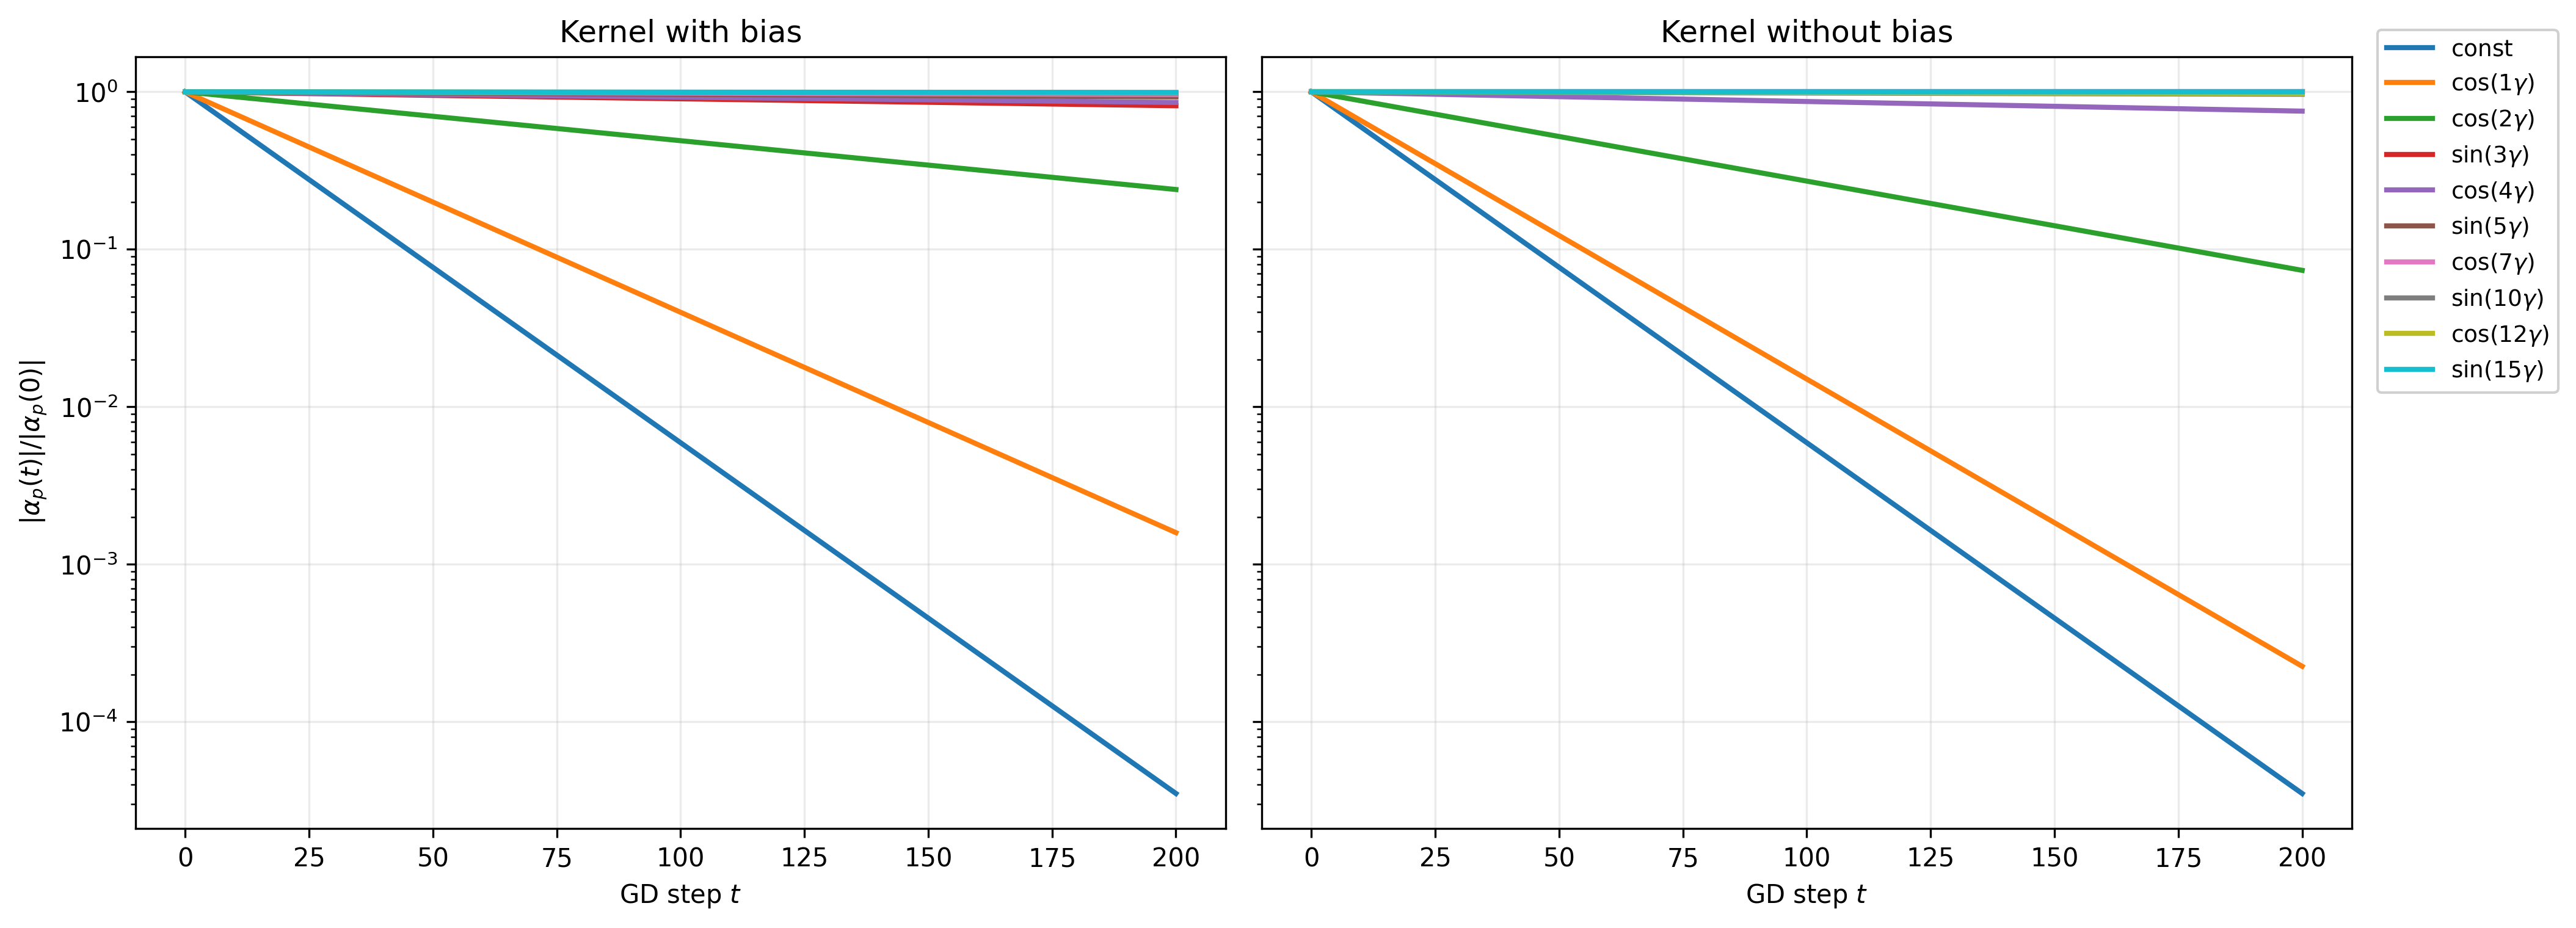
\includegraphics[width=\textwidth]{images/finite_sample_results/story_01_spectral_bias_two_panel_first200.png}
	\caption{Continuum fixed-kernel dynamics for the first \(200\) gradient
		descent steps, comparing the kernel with and without the trainable-bias
		contribution. The curves show normalized mode amplitudes of the residual
		\(|\alpha_p(t)|/|\alpha_p(0)|\) under the diagonal Fourier dynamics.}
	\label{fig:results-continuum-spectral-bias-first200}
\end{figure}

Figure~\ref{fig:results-continuum-odd-modes} isolates odd Fourier modes. With the bias contribution, these modes have nonzero eigenvalues. Without the
bias contribution, the plotted odd modes have zero eigenvalues and remain
constant under the fixed-kernel dynamics.

\begin{figure}[!htbp]
	\centering
	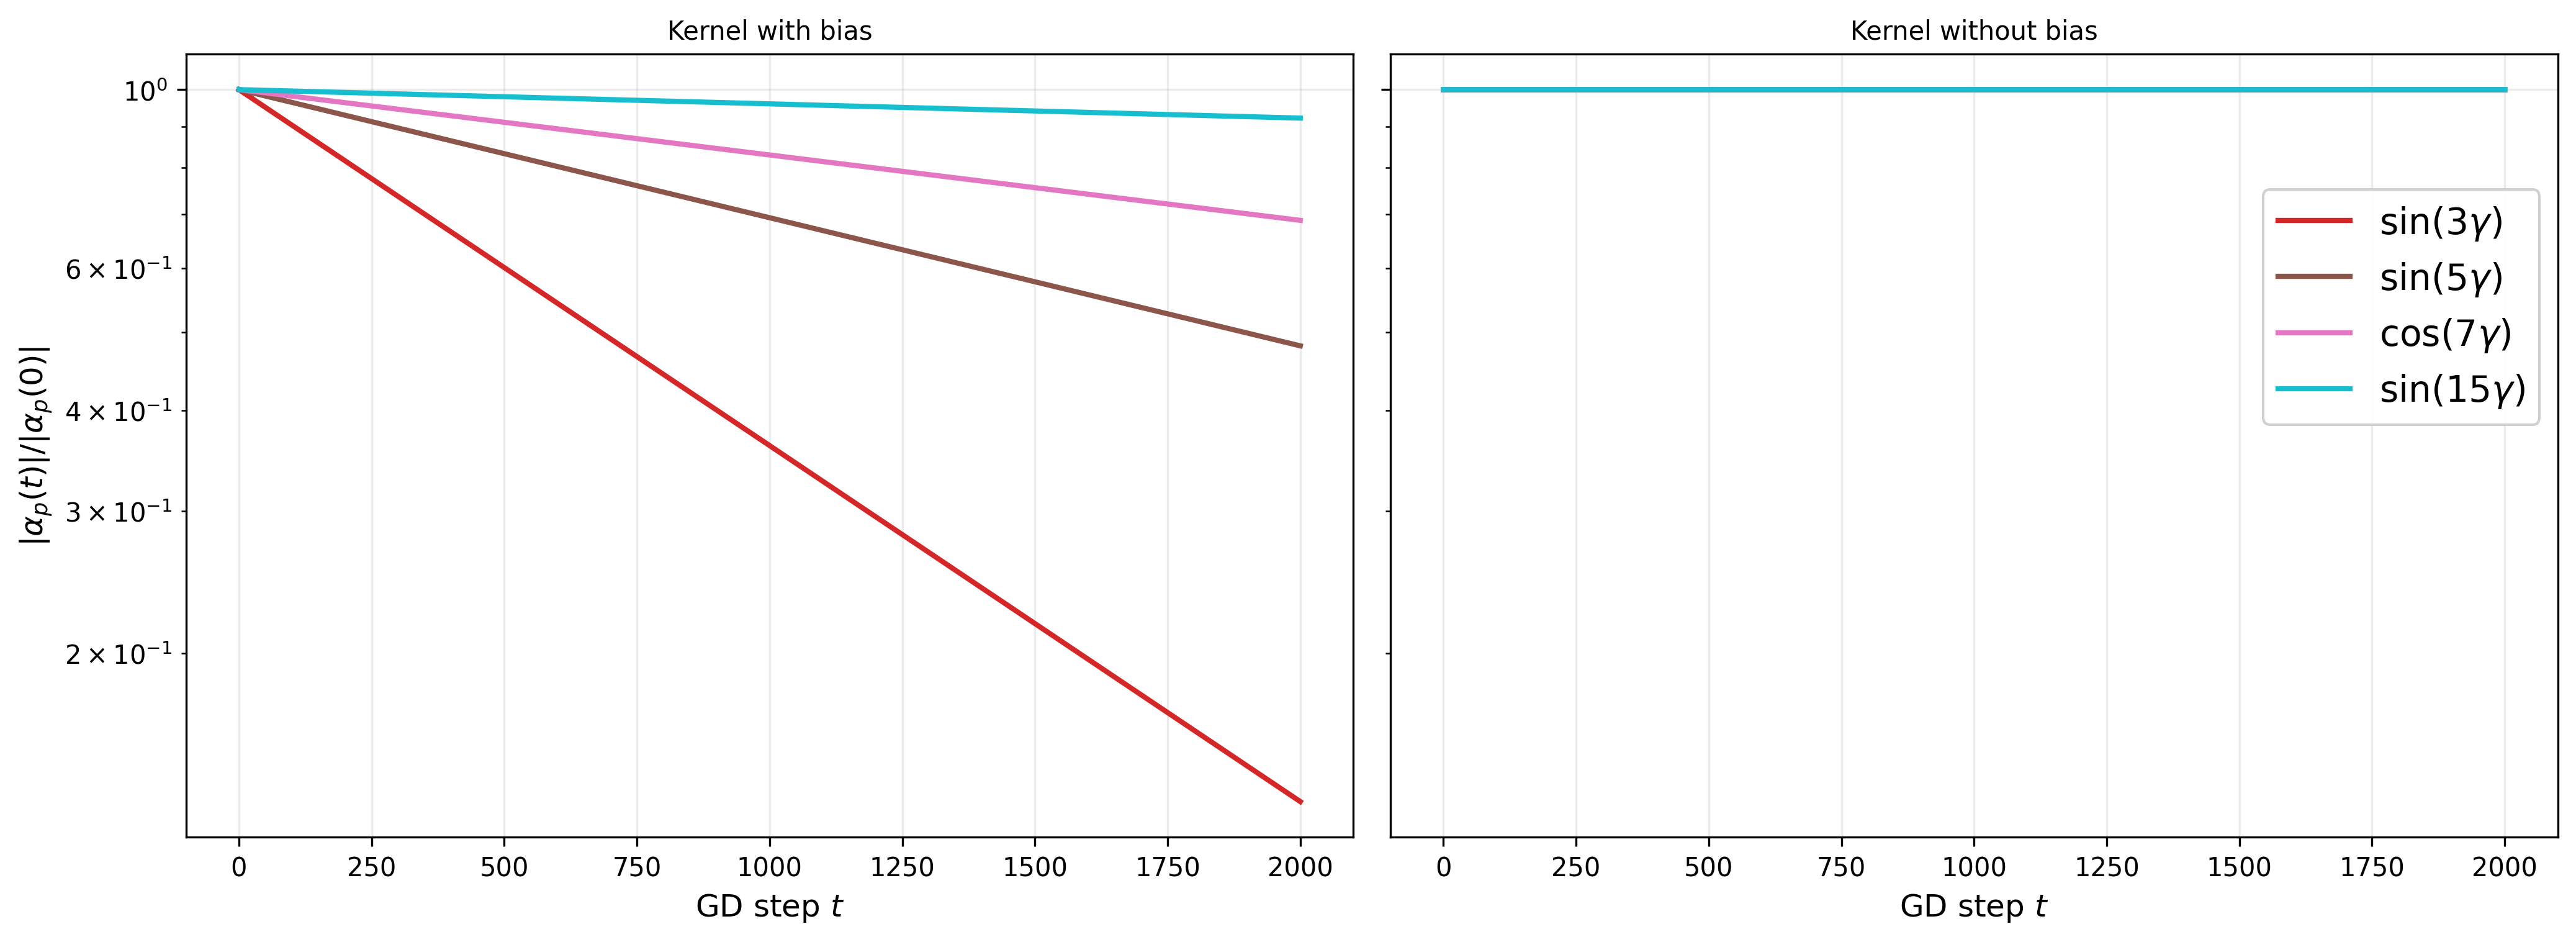
\includegraphics[width=\textwidth]{images/finite_sample_results/story_01_spectral_bias_two_panel_high_freq_odd.png}
	\caption{Odd-mode continuum fixed-kernel dynamics with and without the
		trainable-bias contribution. With the bias contribution, the plotted odd modes
		have nonzero eigenvalues. Without it, the plotted odd modes have zero
		eigenvalues and therefore remain constant under the fixed-kernel dynamics.}
	\label{fig:results-continuum-odd-modes}
\end{figure}

Together, these calculations and plots give the continuum reference case. Here
the operator is the deterministic infinite-width integral operator \(T\), defined
using the uniform measure on \(S^1\). Thus the Fourier frequency subspaces are
exact invariant subspaces of the dynamics, and each residual component decays at
the rate given by the corresponding eigenvalue. This is the standard NTK
spectral mechanism in an explicit setting. Components aligned with larger kernel
eigenvalues decay faster
\citep{jacot2018ntk,lee2020wide,cao2020understandingspectralbiasdeep}. Because
the domain and measure are rotationally symmetric, this eigenvalue ordering is
also a frequency ordering
\citep{bietti2019inductivebiasneuraltangent,basri2019convergence,
	basri2020frequencybiasneuralnetworks}.

With this continuum baseline in place, we now ask how much of this Fourier
structure survives after replacing the uniform measure by finitely many sampled
points.

\section{Finite-sample control on a truncated Fourier subspace}
\label{sec:results-finite-sample}

We now turn to the sampled setting introduced in
section~\ref{sec:finite-sample-methodology}. Throughout, \(K\geq 1\) is fixed,
\(d=2K+1\), and the truncated Fourier subspace \(\mathcal H_K\) is given by
\eqref{eq:method-low-frequency-subspace}. Recall from
Section~\ref{subsec:real-fourier-basis-truncates-subspaces} that, for a basis
function in \(\mathcal H_K\), its frequency means its Fourier index. Thus
\(\phi_0\) has frequency \(0\), corresponding to the constant mode, while both
\(\phi_{k,c}\) and \(\phi_{k,s}\) have frequency \(k\). The matrices
\(\Phi\), \(A\), \(G\), and \(H\) are defined in
\eqref{eq:method-feature-matrix}--\eqref{eq:method-compressed-operator}.

For each basis index \(p\), let \(k(p)\) denote the frequency of the corresponding basis
function \(\phi_p\), and write
\[
	\lambda_p:=\lambda_{k(p)}.
\]

\begin{proposition}[Expectation of the restricted sampled operator]
	\label{prop:results-expectation-H}
	Define
	\begin{equation}
		\lambda_p^{(n)}
		=
		\left(1-\frac{1}{n}\right)\lambda_p+\frac{\Theta(0)}{n},
		\label{eq:results-finite-sample-corrected-eigs}
	\end{equation}
	and let
	\begin{equation}
		\Lambda^{(n)}=\operatorname{diag}(\lambda_p^{(n)}).
		\label{eq:results-finite-sample-eigenvalue-matrix}
	\end{equation}
	Then
	\begin{equation}
		\mathbb E[H]=\Lambda^{(n)}.
		\label{eq:results-expected-H}
	\end{equation}
\end{proposition}

The detailed proof is provided in Appendix~\ref{sec:app-expected-H}.

The finite-sample eigenvalue \(\lambda_p^{(n)}\) differs from the continuum
value \(\lambda_p\) by a term of order \(\frac{\Theta(0)}{n}\). This correction
shrinks with \(n\), so the sampled eigenvalues approach the continuum values as
the sample size grows. For the kernel values and block dimensions used in the
experiments, this correction is small once \(n\) is a few hundred.

The next theorem gives explicit concentration bounds for the three sampled quantities that
appear in the methodology chapter.

\begin{theorem}[Finite-sample concentration on the truncated Fourier subspace]
	\label{thm:results-finite-sample-concentration}
	Assume that
	\begin{equation}
		\kappa:=\sup_{\theta\in[0,2\pi)}|\Theta(\theta)|<\infty.
		\label{eq:results-kappa}
	\end{equation}
	Then, for every \(\varepsilon>0\),
	\begin{equation}
		\mathbb P\!\left(\|G-I_d\|_{\max}\ge \varepsilon\right)
		\le
		d(d+1)\exp\!\left(-\frac{n\varepsilon^2}{4+\frac43\varepsilon}\right),
		\label{eq:results-gram-concentration}
	\end{equation}
	\begin{equation}
		\mathbb P\!\left(\|H-\Lambda^{(n)}\|_{\max}\ge \varepsilon\right)
		\le
		2d^2\exp\!\left(-\frac{n\varepsilon^2}{32\kappa^2}\right),
		\label{eq:results-H-concentration}
	\end{equation}
	and, for \(n\ge 2\),
	\begin{equation}
		\mathbb P\!\left(\|A\Phi-\Phi\Lambda^{(n)}\|_{\max}\ge \varepsilon\right)
		\le
		2nd\exp\!\left(-\frac{n\varepsilon^2}{2\kappa^2+2\kappa\varepsilon}\right).
		\label{eq:results-APhi-concentration}
	\end{equation}
\end{theorem}

The detailed proofs of the three bounds are provided in
Appendix~\ref{app:finite-sample-proofs}.

Combining the preceding concentration bounds gives a single high-probability
event on which all three finite-sample quantities are controlled at once.
Namely, with probability at least \(1-\delta\),
\[
	\|G-I_d\|_{\max},
	\qquad
	\|H-\Lambda^{(n)}\|_{\max},
	\qquad
	\|A\Phi-\Phi\Lambda^{(n)}\|_{\max}
\]
are all of order
\[
	O \left(  \sqrt{\frac{\log(nd/\delta)}{n}}\right) ,
\]
up to logarithmic-over-\(n\) terms and constants depending on the kernel bound
\(\kappa\). Thus the same sampled points simultaneously make the sampled
Fourier basis nearly orthonormal, the compressed operator nearly diagonal, and
the sampled operator action close to its corrected diagonal form. The explicit
version with constants is given in Appendix~\ref{sec:app-simultaneous-proof}.

Theorem~\ref{thm:results-finite-sample-concentration} shows that the sampled
operator remains close to the continuum Fourier decomposition on the truncated
subspace \(\mathcal H_K\). To express this directly at the level of the induced
matrix on Fourier coefficients, define
\begin{equation}
	C:=G^{-1}H,
	\label{eq:results-restricted-operator}
\end{equation}
whenever \(G\) is invertible.

The factor \(G^{-1}\) appears because the sampled Fourier basis is not exactly
orthonormal under the empirical inner product. Thus, when \(G\) is close to
\(I_d\) and \(H\) is close to \(\Lambda^{(n)}\), the coefficient-level
restricted operator \(C=G^{-1}H\) is close to the diagonal finite-sample
prediction \(\Lambda^{(n)}\).

\subsection{Empirical validation of finite-sample Fourier structure}
\label{subsec:results-finite-sample-validation}

The finite-sample bounds above give a target-independent test of whether the
sampled operator still preserves the continuum Fourier structure on the
truncated subspace \(\mathcal H_K\). The three errors have different roles. The
Gram error \(\|G-I_d\|_{\max}\) measures how close the sampled Fourier basis is
to being orthonormal on the sampled points. The compressed-operator error
\(\|H-\Lambda^{(n)}\|_{\max}\) measures how close the sampled operator is to
the diagonal finite-sample prediction on the retained Fourier coordinates. The
action error \(\|A\Phi-\Phi\Lambda^{(n)}\|_{\max}\) measures whether applying
the sampled operator to sampled Fourier modes produces the predicted mode-wise
action.

Figure~\ref{fig:results-finite-sample-diagnostics} shows the empirical behavior
of these three errors appearing in
Theorem~\ref{thm:results-finite-sample-concentration}. All three errors
decrease as \(n\) increases. The plotted high-probability envelopes are
conservative, but they have the same decreasing trend.

\begin{figure}[!htbp]
	\centering

	\begin{subfigure}[t]{0.48\textwidth}
		\centering
		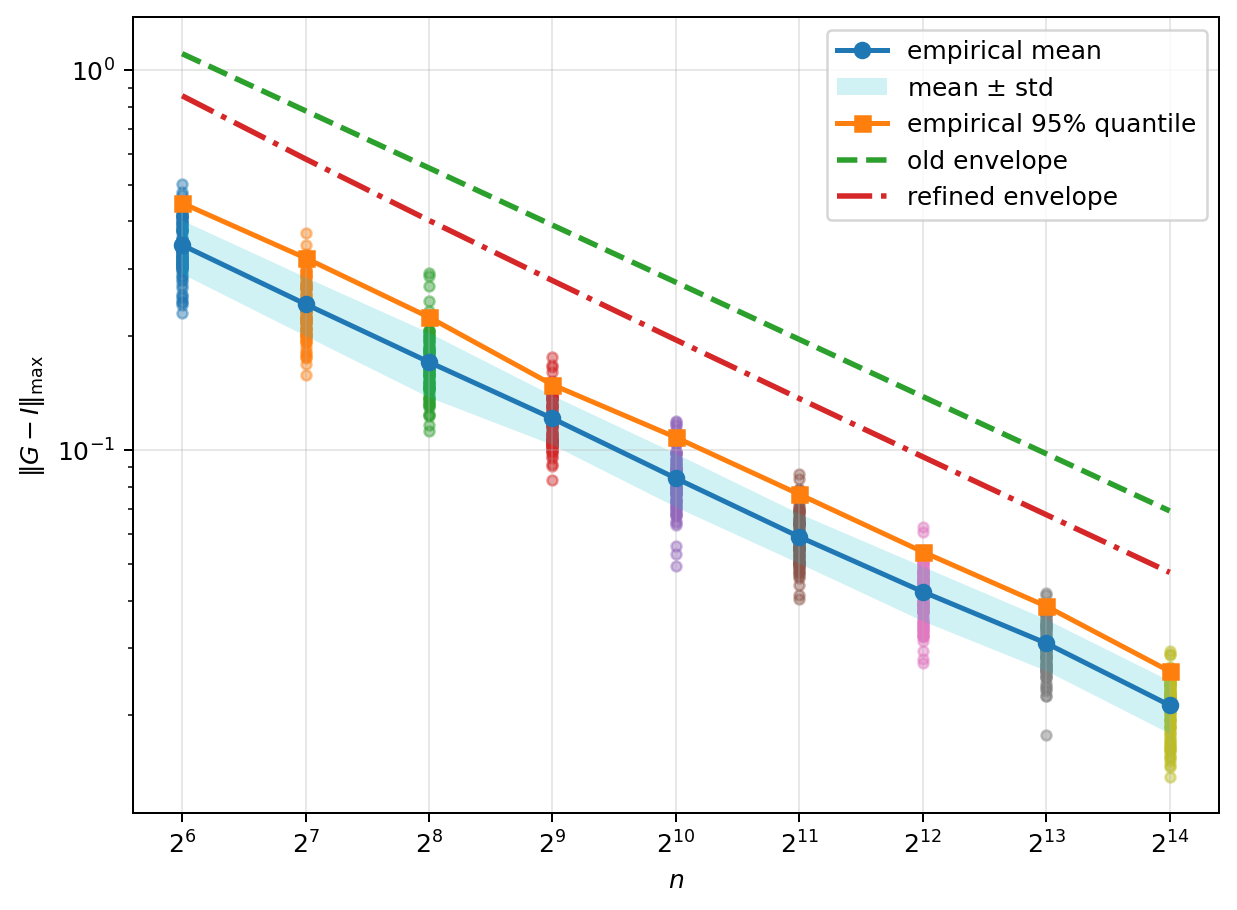
\includegraphics[width=\textwidth]{images/finite_sample_results/theory_envelope_compare_gram_err_max.png}
		\caption{\(\|G-I_d\|_{\max}\)}
	\end{subfigure}
	\hfill
	\begin{subfigure}[t]{0.48\textwidth}
		\centering
		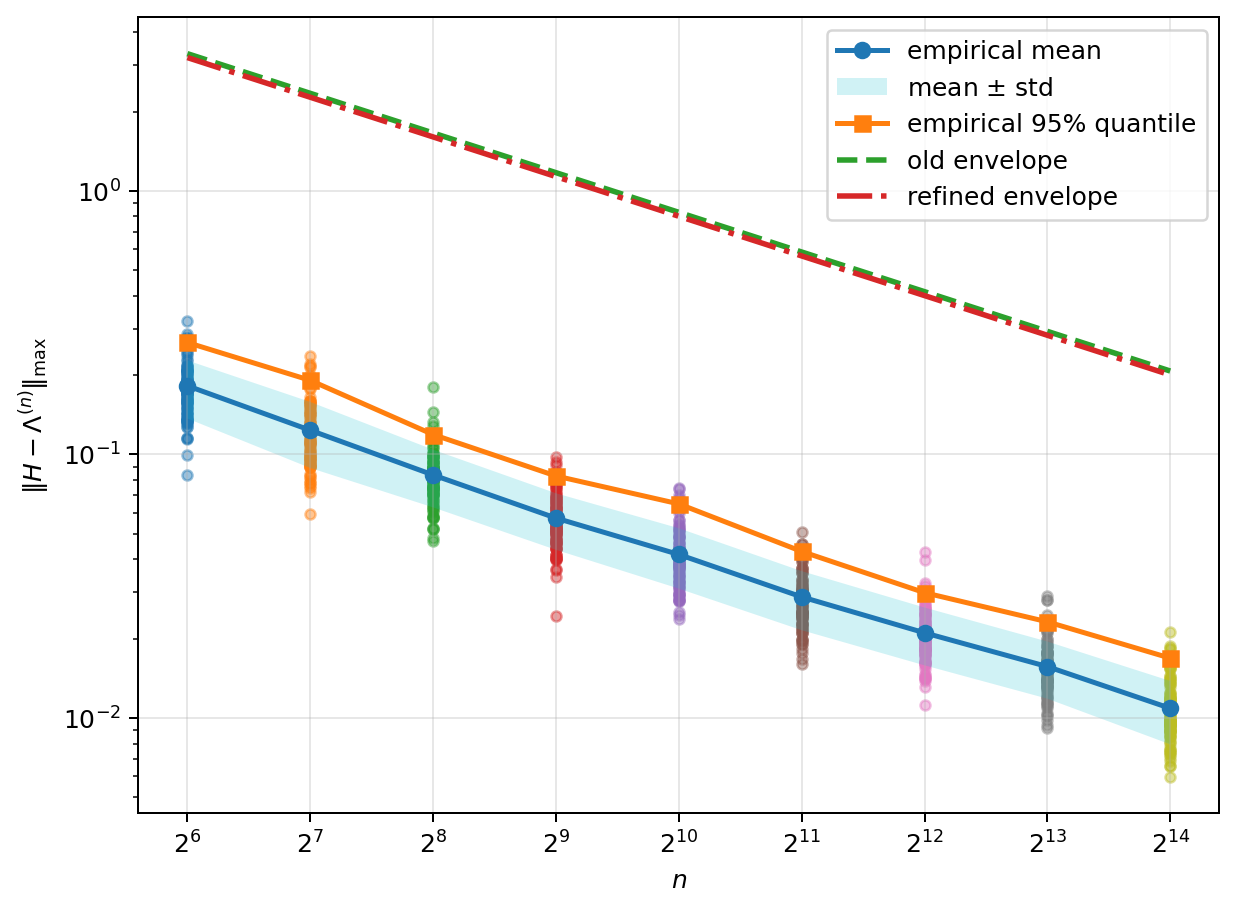
\includegraphics[width=\textwidth]{images/finite_sample_results/theory_envelope_compare_comp_err_max.png}
		\caption{\(\|H-\Lambda^{(n)}\|_{\max}\)}
	\end{subfigure}

	\vspace{0.8em}

	\begin{subfigure}[t]{0.48\textwidth}
		\centering
		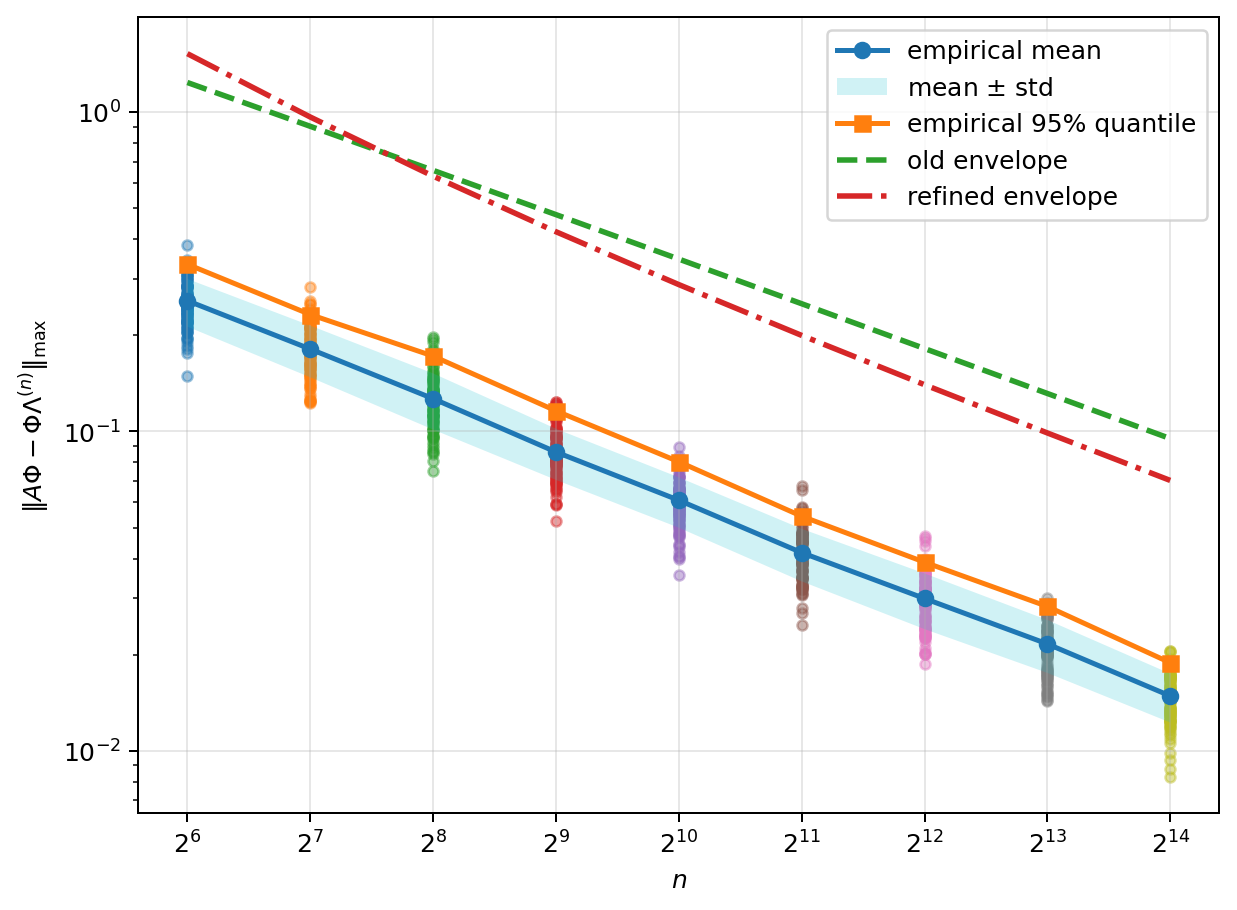
\includegraphics[width=\textwidth]{images/finite_sample_results/theory_envelope_compare_action_err_max.png}
		\caption{\(\|A\Phi-\Phi\Lambda^{(n)}\|_{\max}\)}
	\end{subfigure}

	\caption{Finite-sample diagnostics for the sampled Fourier approximation.
		The three plotted errors decrease with \(n\). The theoretical envelopes are
		conservative, but they show the same decreasing trend.}
	\label{fig:results-finite-sample-diagnostics}
\end{figure}

These bounds naturally lead to the question of what finite sampling does to the
residual dynamics. In the continuum setting,
\eqref{eq:results-continuum-gradient-flow-mode-decay} shows that Fourier
components decay independently. On the retained subspace, this gives the
coefficient system
\[
	\dot\alpha(t)=-\Lambda\alpha(t).
\]
After sampling, if the residual is mainly represented in the retained Fourier
span, then
\[
	\widehat r(t)\approx \Phi\alpha(t),
\]
and the sampled kernel dynamics
\[
	\dot{\widehat r}(t)=-A\widehat r(t)
\]
gives
\[
	\Phi\dot\alpha(t)\approx -A\Phi\alpha(t).
\]
Using the finite-sample decomposition
\[
	A\Phi
	=
	\Phi\Lambda^{(n)}
	+
	\bigl(A\Phi-\Phi\Lambda^{(n)}\bigr),
\]
we obtain
\[
	\Phi\dot\alpha(t)
	\approx
	\underbrace{-\Phi\Lambda^{(n)}\alpha(t)}
	_{\text{finite-sample eigenvalue prediction}}
	\underbrace{
		-\bigl(A\Phi-\Phi\Lambda^{(n)}\bigr)\alpha(t)
	}_{\text{finite-sample action error}} .
\]
If the action-error term were zero, each retained Fourier component would follow
\begin{equation}
	\alpha_p(t)
	=
	\exp(-\lambda_p^{(n)}t)\alpha_p(0)
	\label{eq:finite-sample-eigenvalue-prediction}
\end{equation}

The action-error term is small by the finite-sample bounds, but it is not zero.
To see when it can become visible, suppose that the retained coefficients are
normalized so that \(\alpha_p(0)=1\) for all retained basis indices \(p\) in \(\mathcal H_K\), and
suppose initially that they follow the finite-sample eigenvalue prediction from \eqref{eq:finite-sample-eigenvalue-prediction}.
Then
\[
	\alpha(t)
	\approx
	\exp(-\Lambda^{(n)}t)\mathbf 1,
\]
and hence
\[
	\widehat r(t)
	\approx
	\Phi\exp(-\Lambda^{(n)}t)\mathbf 1
	=
	\sum_p \exp(-\lambda_p^{(n)}t)\Phi_p,
\]
where \(\Phi_p\) is the sampled vector of the \(p\)-th retained Fourier basis
function and \(\mathbf 1\in\mathbb R^d\) is the vector with all entries equal to one.

Substituting this expression into the action-error term gives
\[
	\bigl(A\Phi-\Phi\Lambda^{(n)}\bigr)\alpha(t)
	\approx
	\bigl(A\Phi-\Phi\Lambda^{(n)}\bigr)
	\exp(-\Lambda^{(n)}t)\mathbf 1 .
\]
Therefore
\[
	\left\|
	\bigl(A\Phi-\Phi\Lambda^{(n)}\bigr)\alpha(t)
	\right\|_{\max}
	\le
	\|A\Phi-\Phi\Lambda^{(n)}\|_{\max}
	\sum_p \exp(-\lambda_p^{(n)}t).
\]
This is a crude upper bound on the extra motion caused by finite sampling, and gives a scale at which
deviations from the predicted eigenvalue decay become visible.

For a single retained component \(p\), the eigenvalue prediction gives
\[
	|\alpha_p(t)|
	\approx
	\exp(-\lambda_p^{(n)}t),
	\qquad
	|\dot\alpha_p(t)|
	\approx
	\lambda_p^{(n)}\exp(-\lambda_p^{(n)}t).
\]
Thus, the predicted movement of component \(p\) is \(\lambda_p^{(n)}\exp(-\lambda_p^{(n)}t)\).
This eigenvalue prediction should therefore be reliable while
\[
	\lambda_p^{(n)}\underbrace{\exp(-\lambda_p^{(n)}t)}_{\alpha_p(t)}
	\gg
	\|A\Phi-\Phi\Lambda^{(n)}\|_{\max} \sum_q \underbrace{\exp(-\lambda_q^{(n)}t)}_{\alpha_q(t)}.
\]

The left-hand side is the motion predicted for component \(p\) by its own eigenvalue.
This term becomes small as \(\alpha_p(t)\) decays.
The right-hand side is a bound on the extra motion coming from the
finite-sample action error. This term is small when the action error is small,
but it depends on all retained components, including components that decay more
slowly.

The comparison above suggests a two-stage picture. At early times, the
retained components have not yet decayed much, so the eigenvalue-driven motion
is larger than the finite-sample action error. The sampled curves should
therefore follow the finite-sample eigenvalue prediction. At later times, after
some components have decayed substantially, the same action error can become
visible relative to the remaining motion. Figures~\ref{fig:results-random-sampling-first200}
and~\ref{fig:results-random-sampling-highfreq} show these two regimes for
\(n=4096\) uniformly sampled points.

\begin{figure}[!htbp]
	\centering
	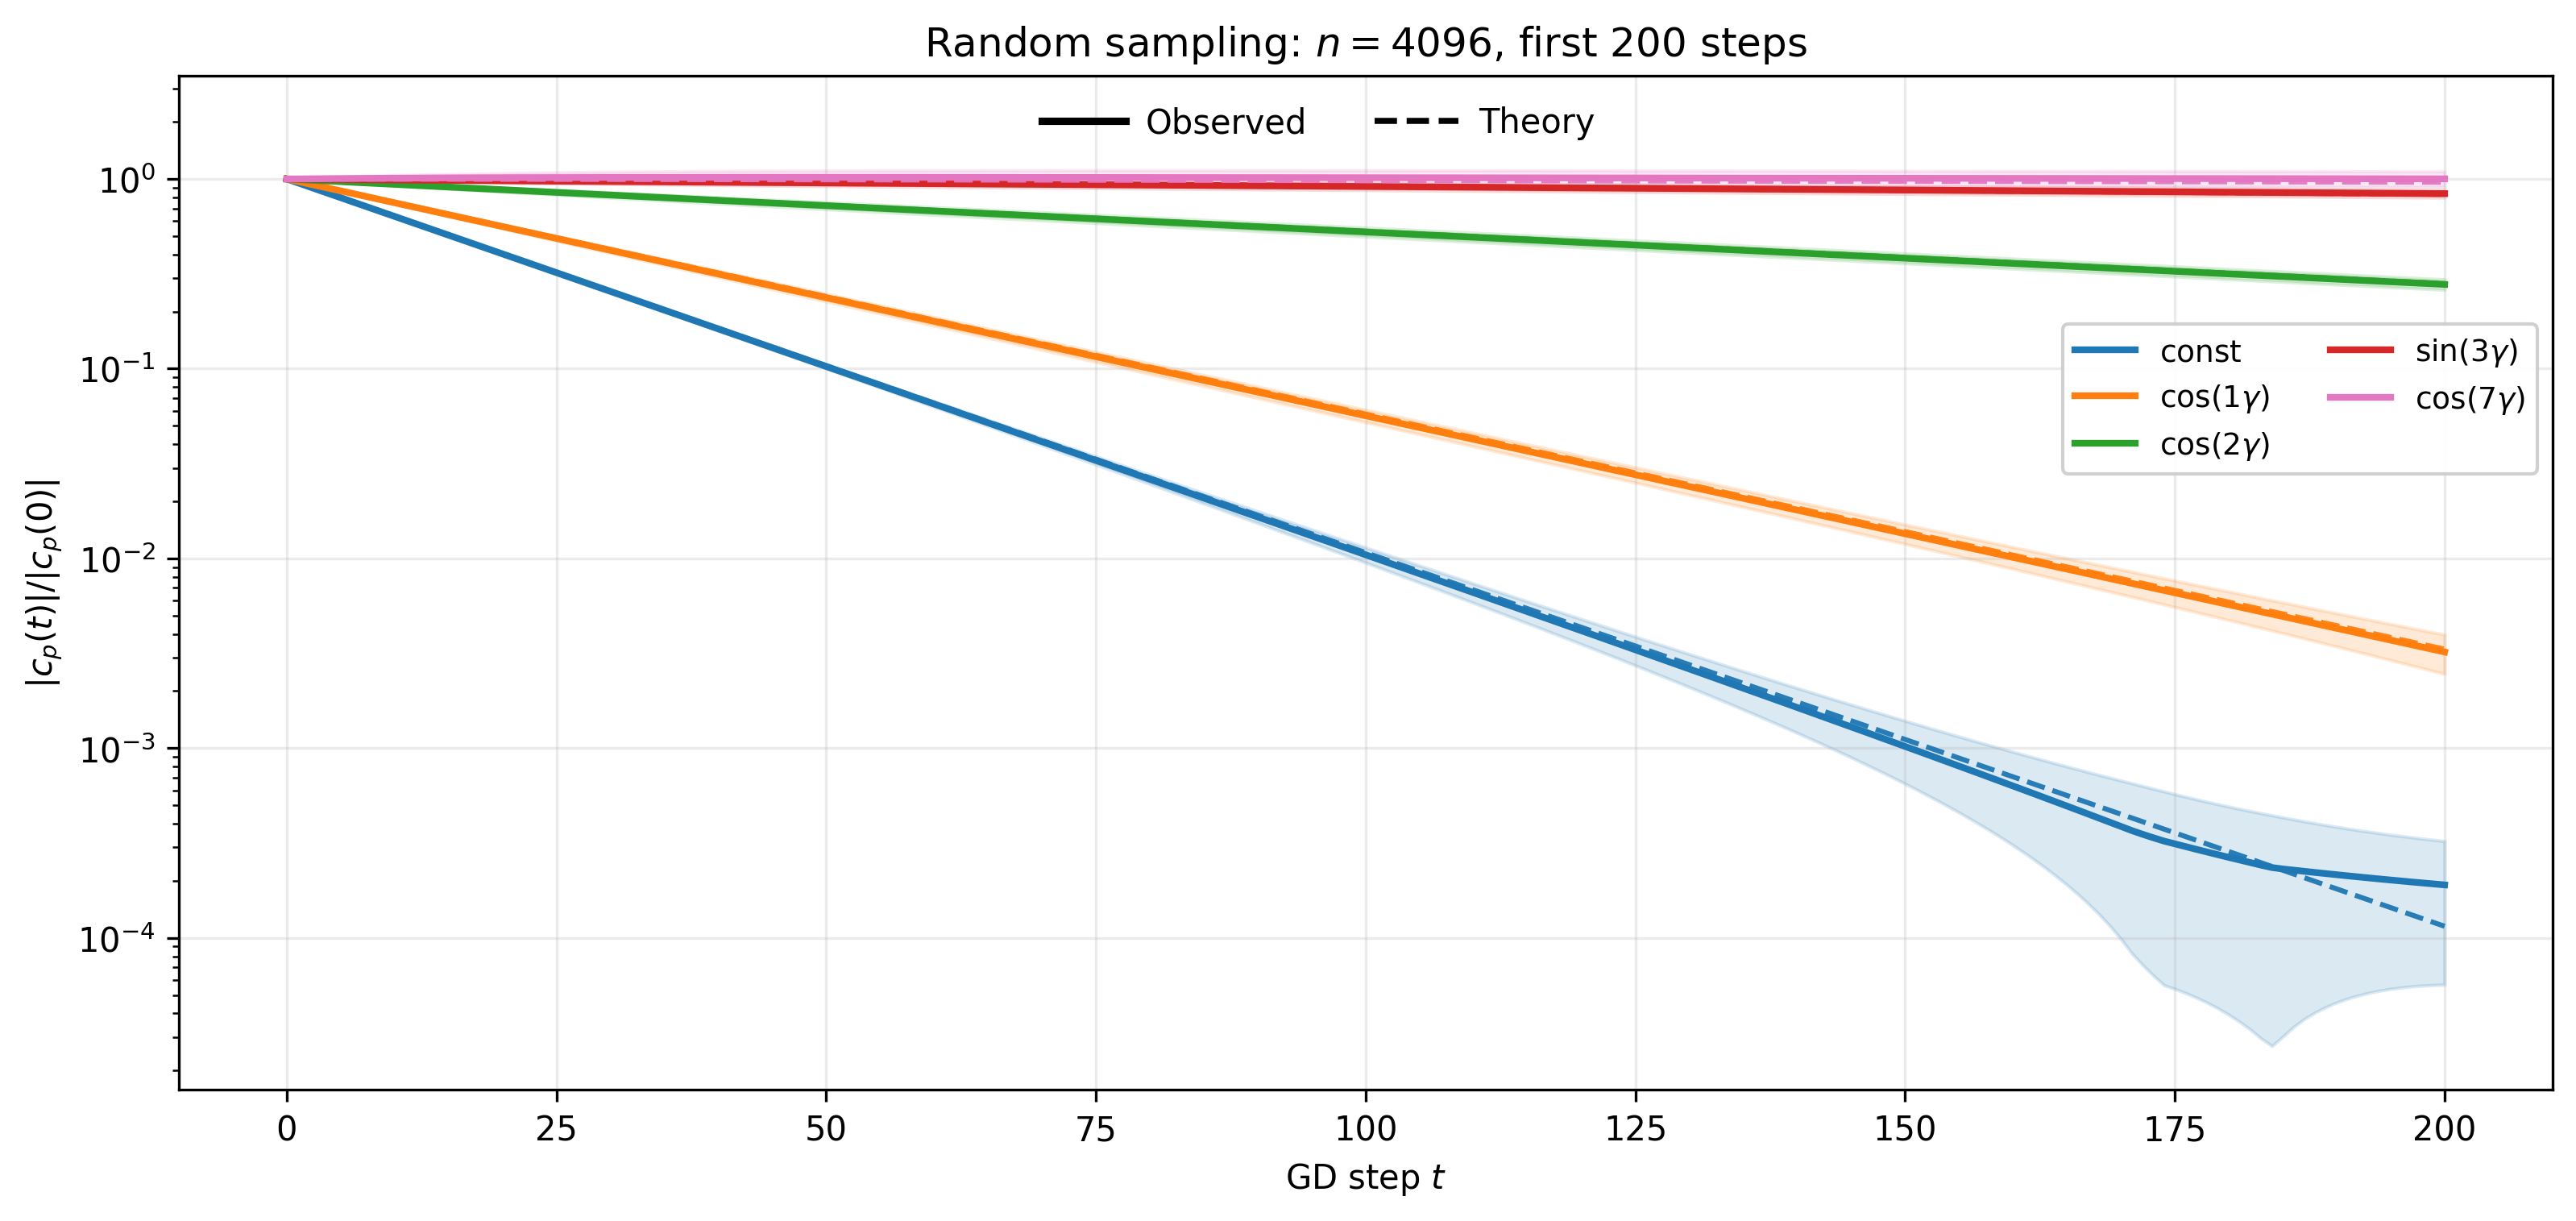
\includegraphics[width=\textwidth]{images/finite_sample_results/story_02_random_n4096_components_first200.png}
	\caption{Random sampling with \(n=4096\), first \(200\) gradient descent
		steps. Solid curves show the observed normalized residual amplitudes
		\(|\alpha_p(t)|/|\alpha_p(0)|\), while dashed curves show the diagonal
		prediction from the finite-sample corrected eigenvalues
		\(\lambda_p^{(n)}\).}
	\label{fig:results-random-sampling-first200}
\end{figure}

\begin{figure}[!htbp]
	\centering
	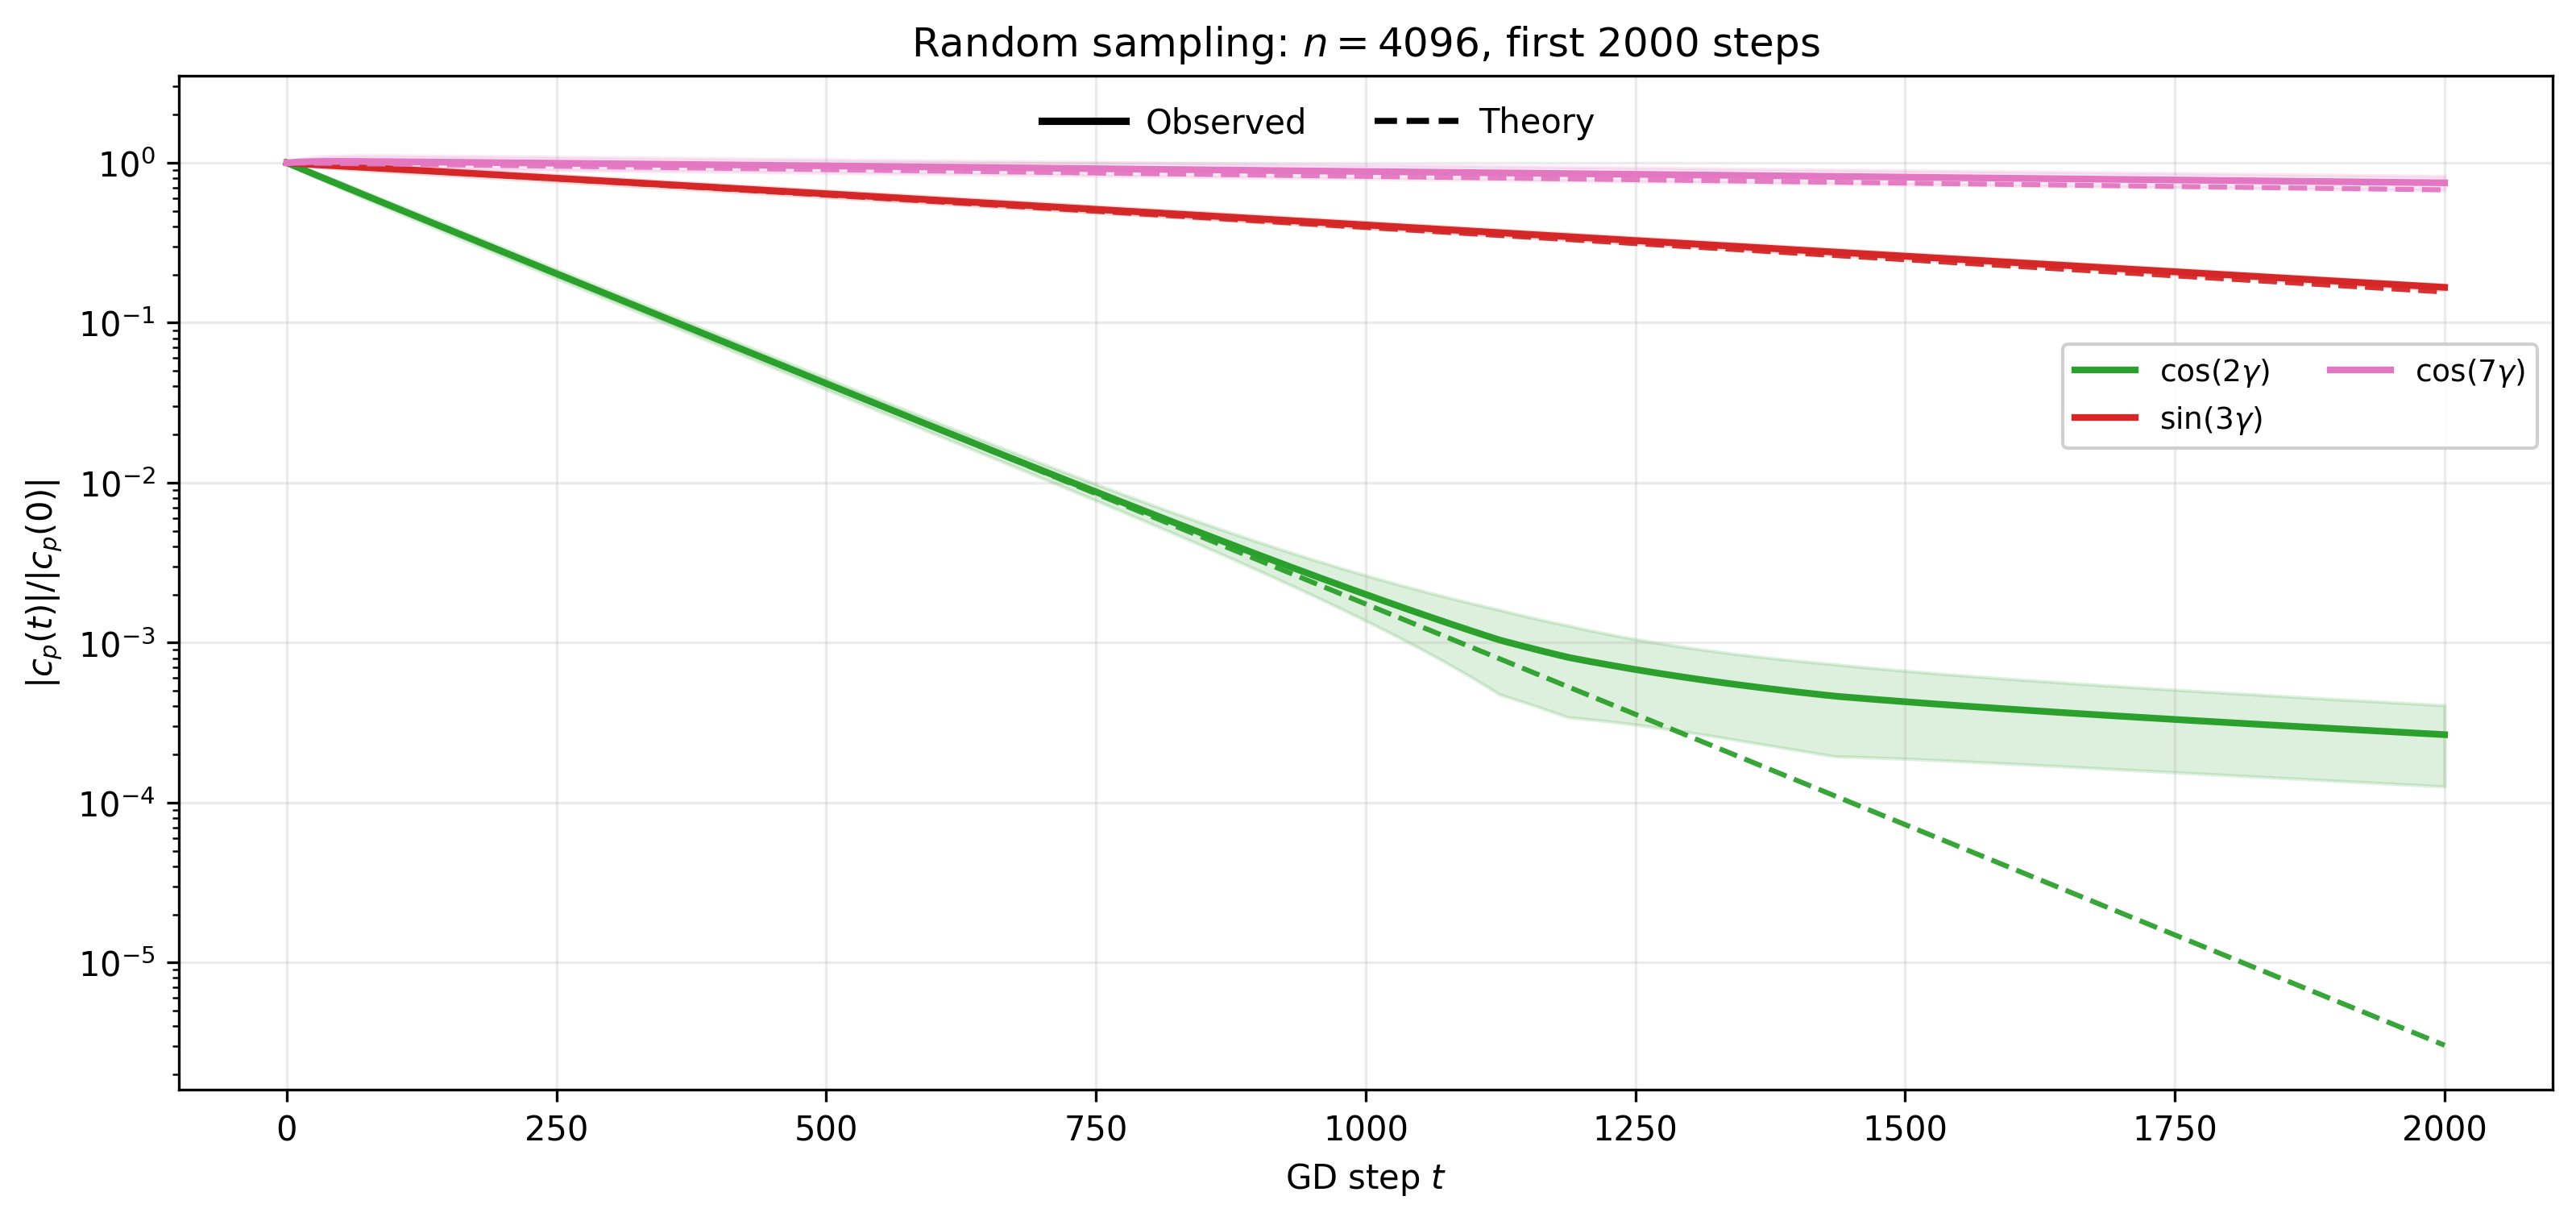
\includegraphics[width=\textwidth]{images/finite_sample_results/story_02_random_n4096_components_all_steps_high_freq_only.png}
	\caption{Random sampling with \(n=4096\), higher-frequency retained modes over
		\(2000\) gradient descent steps. The diagonal prediction captures the initial
		decay rates, while small deviations from this prediction become visible at
		later times.}
	\label{fig:results-random-sampling-highfreq}
\end{figure}

However, the level at which an individual curve starts to flatten cannot be computed
directly from the max-norm bounds in
Theorem~\ref{thm:results-finite-sample-concentration} because these bounds control the
largest possible error over the whole retained Fourier block. They are
therefore useful for explaining why deviations can appear once the predicted
motion becomes small, but they do not determine the deviation level of each
Fourier component separately. That level depends on the actual sampled operator
for the particular draw of training points, and on which other Fourier
components are still present when the component under consideration has already
decayed.

\subsection{Interpretation of the finite-sample results}
\label{subsec:results-finite-sample-interpretation}

The finite-sample results show that the continuum Fourier picture is not only a
population-level statement. For a fixed low-frequency block \(\mathcal H_K\),
random sampling perturbs the Fourier structure in a controlled way. The sampled
basis is not exactly orthonormal, and the sampled Fourier modes are not exact
eigenvectors of the sampled operator, but the errors measured by
\(G-I_d\), \(H-\Lambda^{(n)}\), and
\(A\Phi-\Phi\Lambda^{(n)}\) decrease with \(n\).

This supports the usual NTK spectral-bias mechanism in a finite-sample setting.
In the continuum model, the Fourier modes diagonalize the NTK operator and the
eigenvalues determine the decay rates. The results above show that, on a fixed
retained block, the sampled operator remains close to this diagonal Fourier
description. This complements the population-level harmonic analyses of NTK
spectra on the sphere and circle
\citep{basri2019convergence,bietti2019inductivebiasneuraltangent,
	cao2020understandingspectralbiasdeep,basri2020frequencybiasneuralnetworks}
by making explicit how the same structure survives after replacing the uniform
measure by finitely many sampled points.

The residual experiments then show the dynamical consequence. The corrected
finite-sample eigenvalues \(\lambda_p^{(n)}\) predict the early decay of the
retained Fourier components, while the finite-sample action error explains why
late-time deviations can appear once some components have become small. Thus
finite sampling does not remove the spectral-bias mechanism; it turns the exact
continuum diagonal dynamics into an approximate low-frequency description.

This suggests a direct test. If the decay of each retained component is mainly
governed by its eigenvalue, then an eigenvalue-based rescaling should
remove most of the frequency-dependent decay. The next experiment tests this prediction directly.

\section{Preconditioned sampled dynamics}
\label{sec:results-preconditioned-sampled-dynamics}

We next apply the Fourier-block preconditioning construction from
Section~\ref{sec:method-preconditioning}. The goal is to compare the baseline
sampled dynamics with two block-corrected dynamics: one using the diagonal
finite-sample prediction and one using the observed sampled Fourier block.

\subsection{Experimental setup}
\label{subsec:results-preconditioned-setup}

The three sampled dynamics are
\[
	B_{\mathrm{base}}=A,
	\qquad
	B_{\mathrm{th}}=P_{\mathrm{th}}A,
	\qquad
	B_{\mathrm{emp}}=P_{\mathrm{emp}}A.
\]
Here \(P_{\mathrm{th}}\) is defined in
\eqref{eq:method-theory-preconditioner} and uses the diagonal prediction
\(\Lambda^{(n)}\). The empirical preconditioner \(P_{\mathrm{emp}}\), defined in
\eqref{eq:method-empirical-preconditioner}, uses the observed coefficient-space
block \(C_n^{(K)}=G^{-1}H\).

In this experiment, we use the target
\begin{equation}
	f^*(\gamma)
	=
	1
	+0.9\cos(\gamma)
	+0.5\cos(2\gamma)
	-0.35\sin(3\gamma)
	+0.25\cos(7\gamma).
	\label{eq:results-preconditioned-in-block-target}
\end{equation}
The retained preconditioning block contains all active target frequencies shown
in the residual plots.

\subsection{Mode-wise residual decay}
\label{subsec:results-preconditioned-mode-decay}

Figure~\ref{fig:results-preconditioned-mode-decay} shows the
residual amplitudes for the baseline, theory-preconditioned, and empirically
preconditioned dynamics. The baseline dynamics show separated decay rates
across retained modes. Both preconditioned dynamics reduce this separation, with
the empirical preconditioner giving the flattest curves.

\begin{figure}[!htbp]
	\centering
	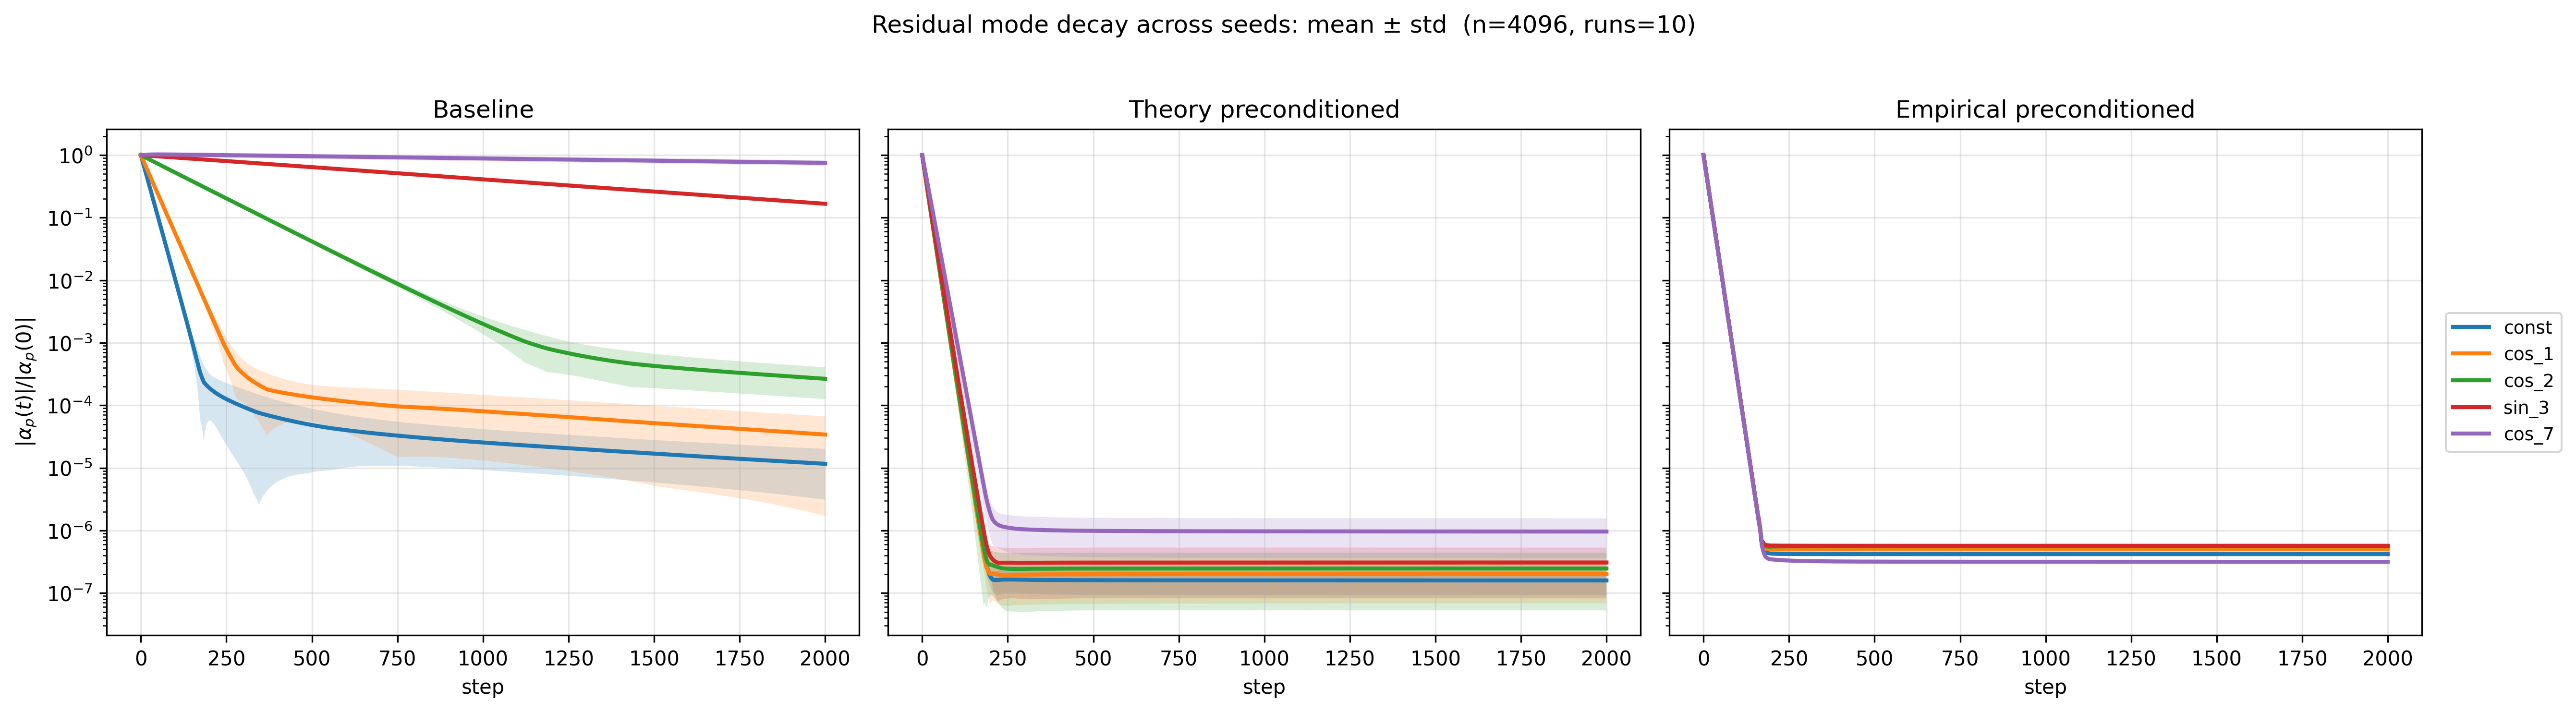
\includegraphics[width=\textwidth]{images/finite_sample_results/all_mode_decay_three_panel_mean_std_n4096.png}
	\caption{Preconditioned sampled dynamics at \(n=4096\). The baseline dynamics
		shows separated decay rates across retained Fourier modes. Both
		preconditioned dynamics make the retained residual amplitudes decay on more
		similar time scales. The empirical preconditioner gives the most uniform
		decay, while the theory preconditioner uses only the predicted diagonal
		scaling.}
	\label{fig:results-preconditioned-mode-decay}
\end{figure}

Figure~\ref{fig:results-preconditioned-probe-fit} compares the final prediction
on a dense probe grid. The baseline fit leaves a visible residual, while both
preconditioned flows more closely match the target.

\begin{figure}[!htbp]
	\centering
	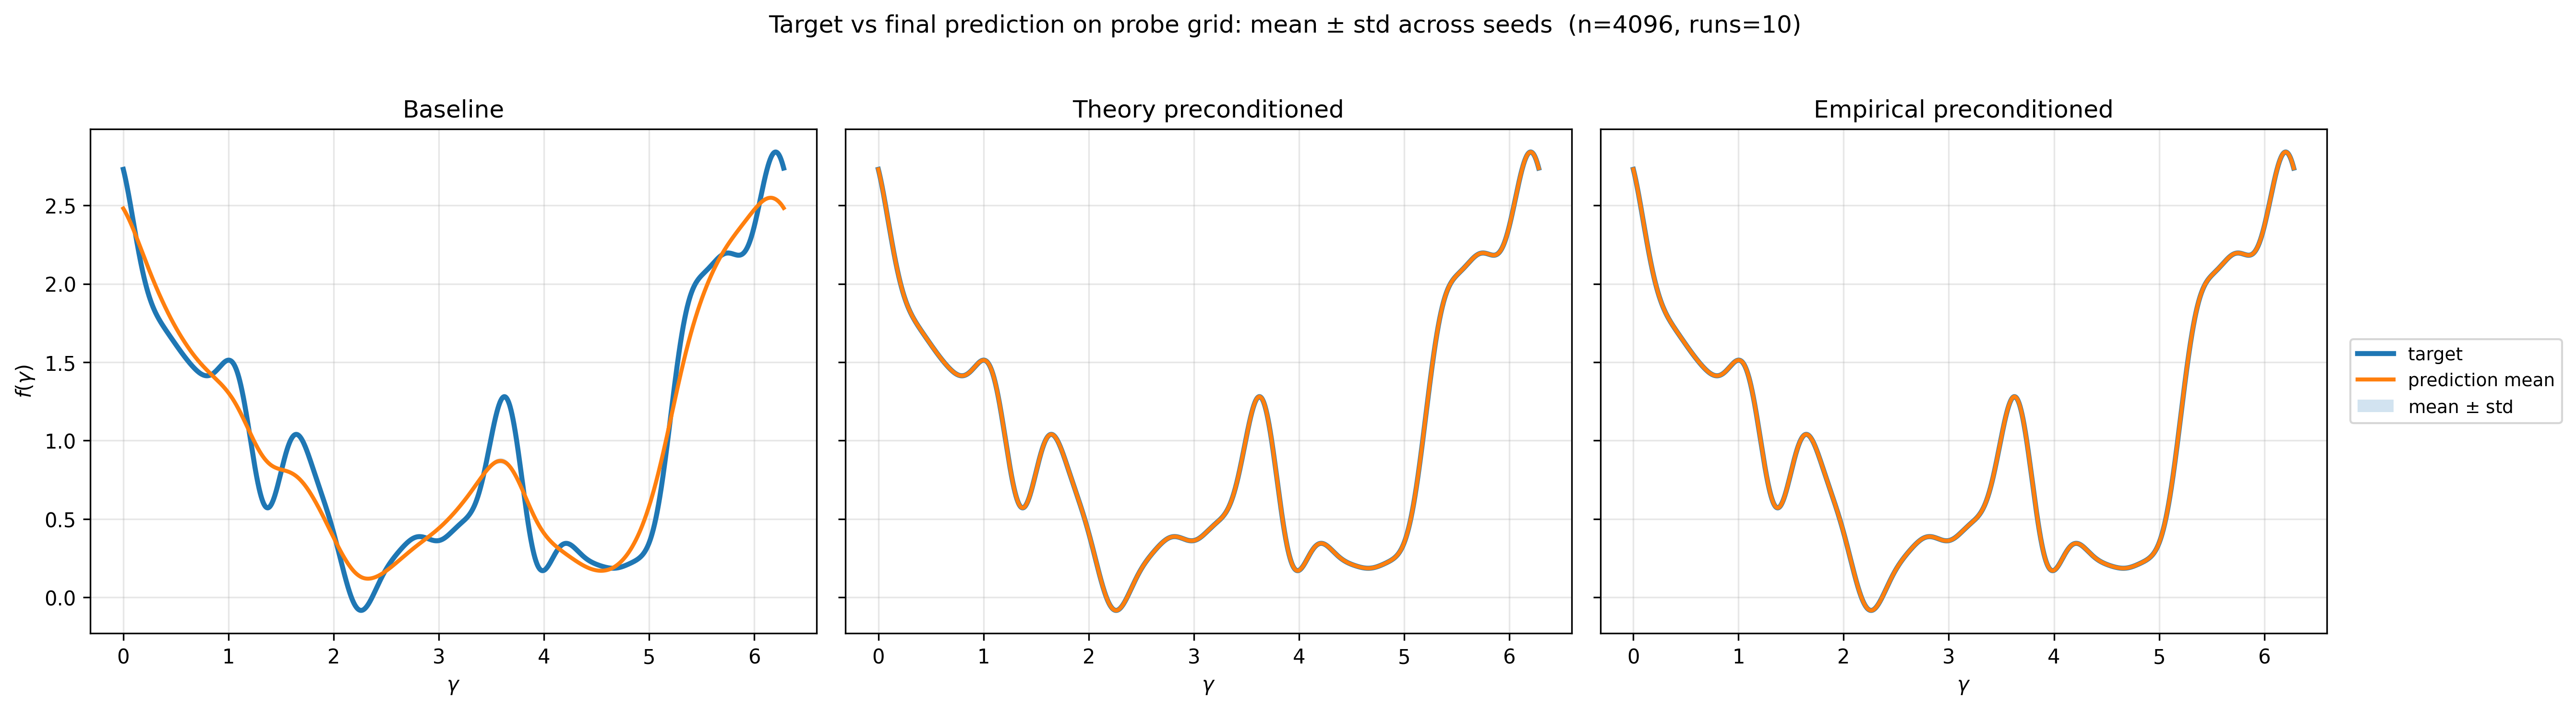
\includegraphics[width=\textwidth]{images/finite_sample_results/probe_target_vs_prediction_three_panel_mean_std_n4096.png}
	\caption{Final prediction on a dense probe grid for the same experiment as
		Figure~\ref{fig:results-preconditioned-mode-decay}. The baseline fit leaves a
		visible residual, while both preconditioned dynamics closely match the target.
		The theory and empirical preconditioners are nearly indistinguishable at the
		level of the final fitted function.}
	\label{fig:results-preconditioned-probe-fit}
\end{figure}

\subsection{Theory versus empirical preconditioning}
\label{subsec:results-theory-vs-empirical-preconditioning}

Figure~\ref{fig:results-theory-precond-spectrum} shows the spectrum obtained
after applying the theory preconditioner to the sampled Fourier block. At the
coefficient level, the empirical block is \(C=G^{-1}H\). The empirical
preconditioner would invert this block directly, giving \(C_{\mathrm{emp}}^{-1}C=I_d\),
so all eigenvalues would be equal to \(1\). The theory preconditioner instead rescales
by the predicted diagonal eigenvalues \(\Lambda^{(n)}\). Thus it is exact only
when \(C=\Lambda^{(n)}\). The figure shows that, as \(n\) increases, the
theory-preconditioned spectrum moves closer to the ideal value \(1\). This is
the empirical counterpart of the finite-sample bounds above: the sampled block
\(C\) approaches the diagonal prediction \(\Lambda^{(n)}\), so the diagonal
theory preconditioner becomes a better approximation to the empirical block
inverse.

\begin{figure}[!htbp]
	\centering
	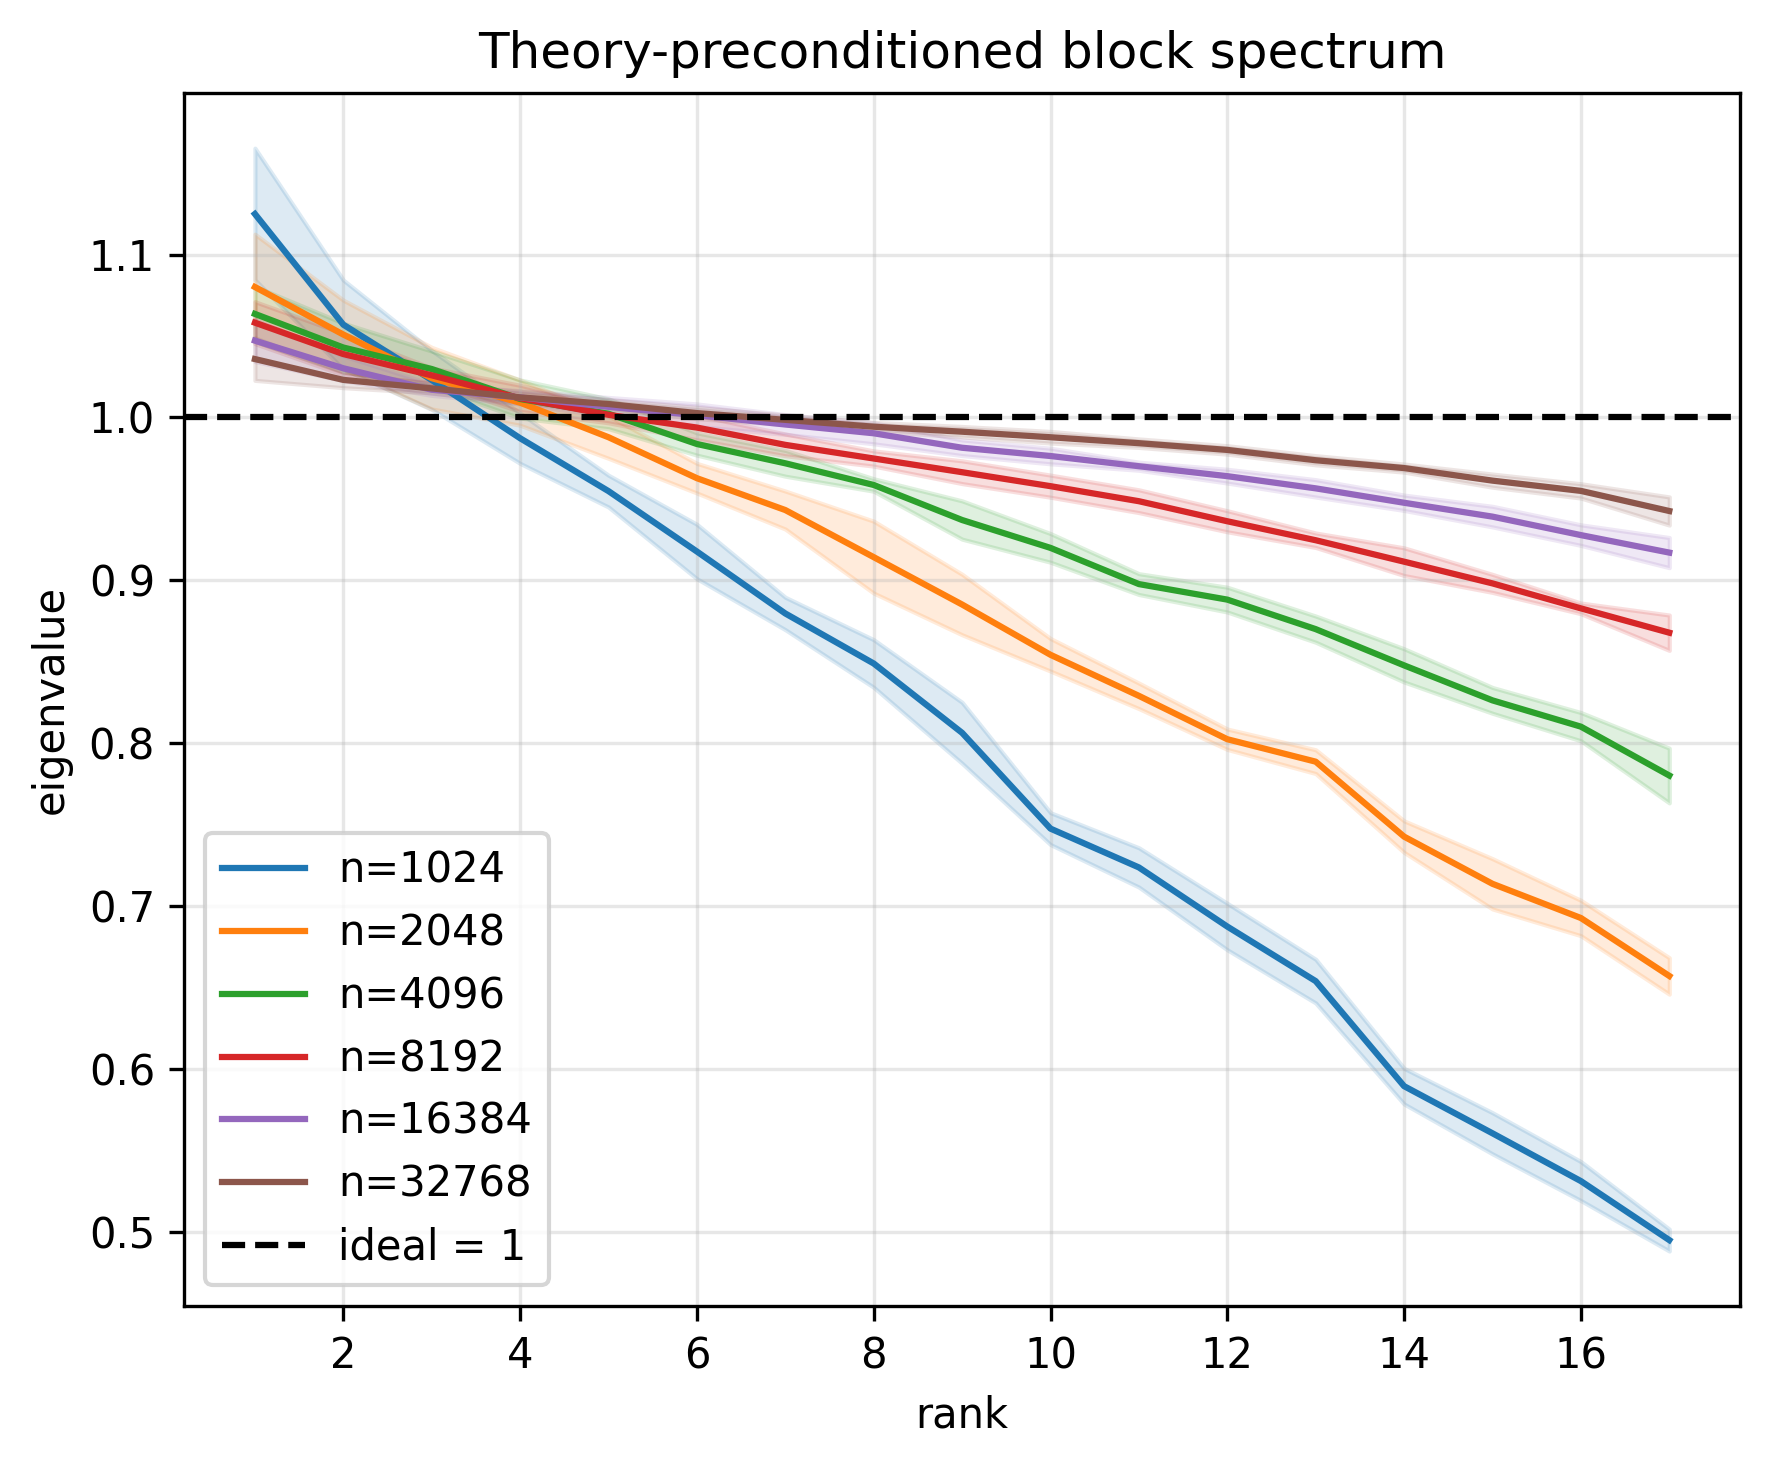
\includegraphics[width=0.72\textwidth]{images/finite_sample_results/theory_preconditioned_spectrum_all_n.png}
	\caption{Spectrum of the theory-preconditioned sampled Fourier block as a
		function of sample size. If the theory preconditioner exactly inverted the
		sampled block, all eigenvalues would be equal to \(1\). As \(n\) increases,
		the spectrum becomes flatter and moves closer to this ideal value.}
	\label{fig:results-theory-precond-spectrum}
\end{figure}

Figure~\ref{fig:results-preconditioner-gap} compares the theory and empirical
constructions at two levels. The preconditioner \(P\) is an operator on sampled
function values. Given a vector in \(\mathbb R^n\), it projects that vector onto
the retained Fourier block, rescales the retained Fourier coefficients, and
maps the result back to \(\mathbb R^n\). Thus, the gap between
\(P_{\mathrm{th}}\) and \(P_{\mathrm{emp}}\) measures how different the two
correction steps are before they are combined with the sampled kernel operator.

The product \(PA\) is the operator that is actually used in the residual
dynamics. It first applies the sampled kernel operator \(A\) to the residual,
and then applies the correction \(P\) to the retained Fourier components of the
result. Thus, the gap between \(B_{\mathrm{th}}\) and \(B_{\mathrm{emp}}\)
measures how different the resulting training dynamics are. Both gaps decrease
with sample size.

\begin{figure}[!htbp]
	\centering

	\begin{subfigure}[t]{0.48\textwidth}
		\centering
		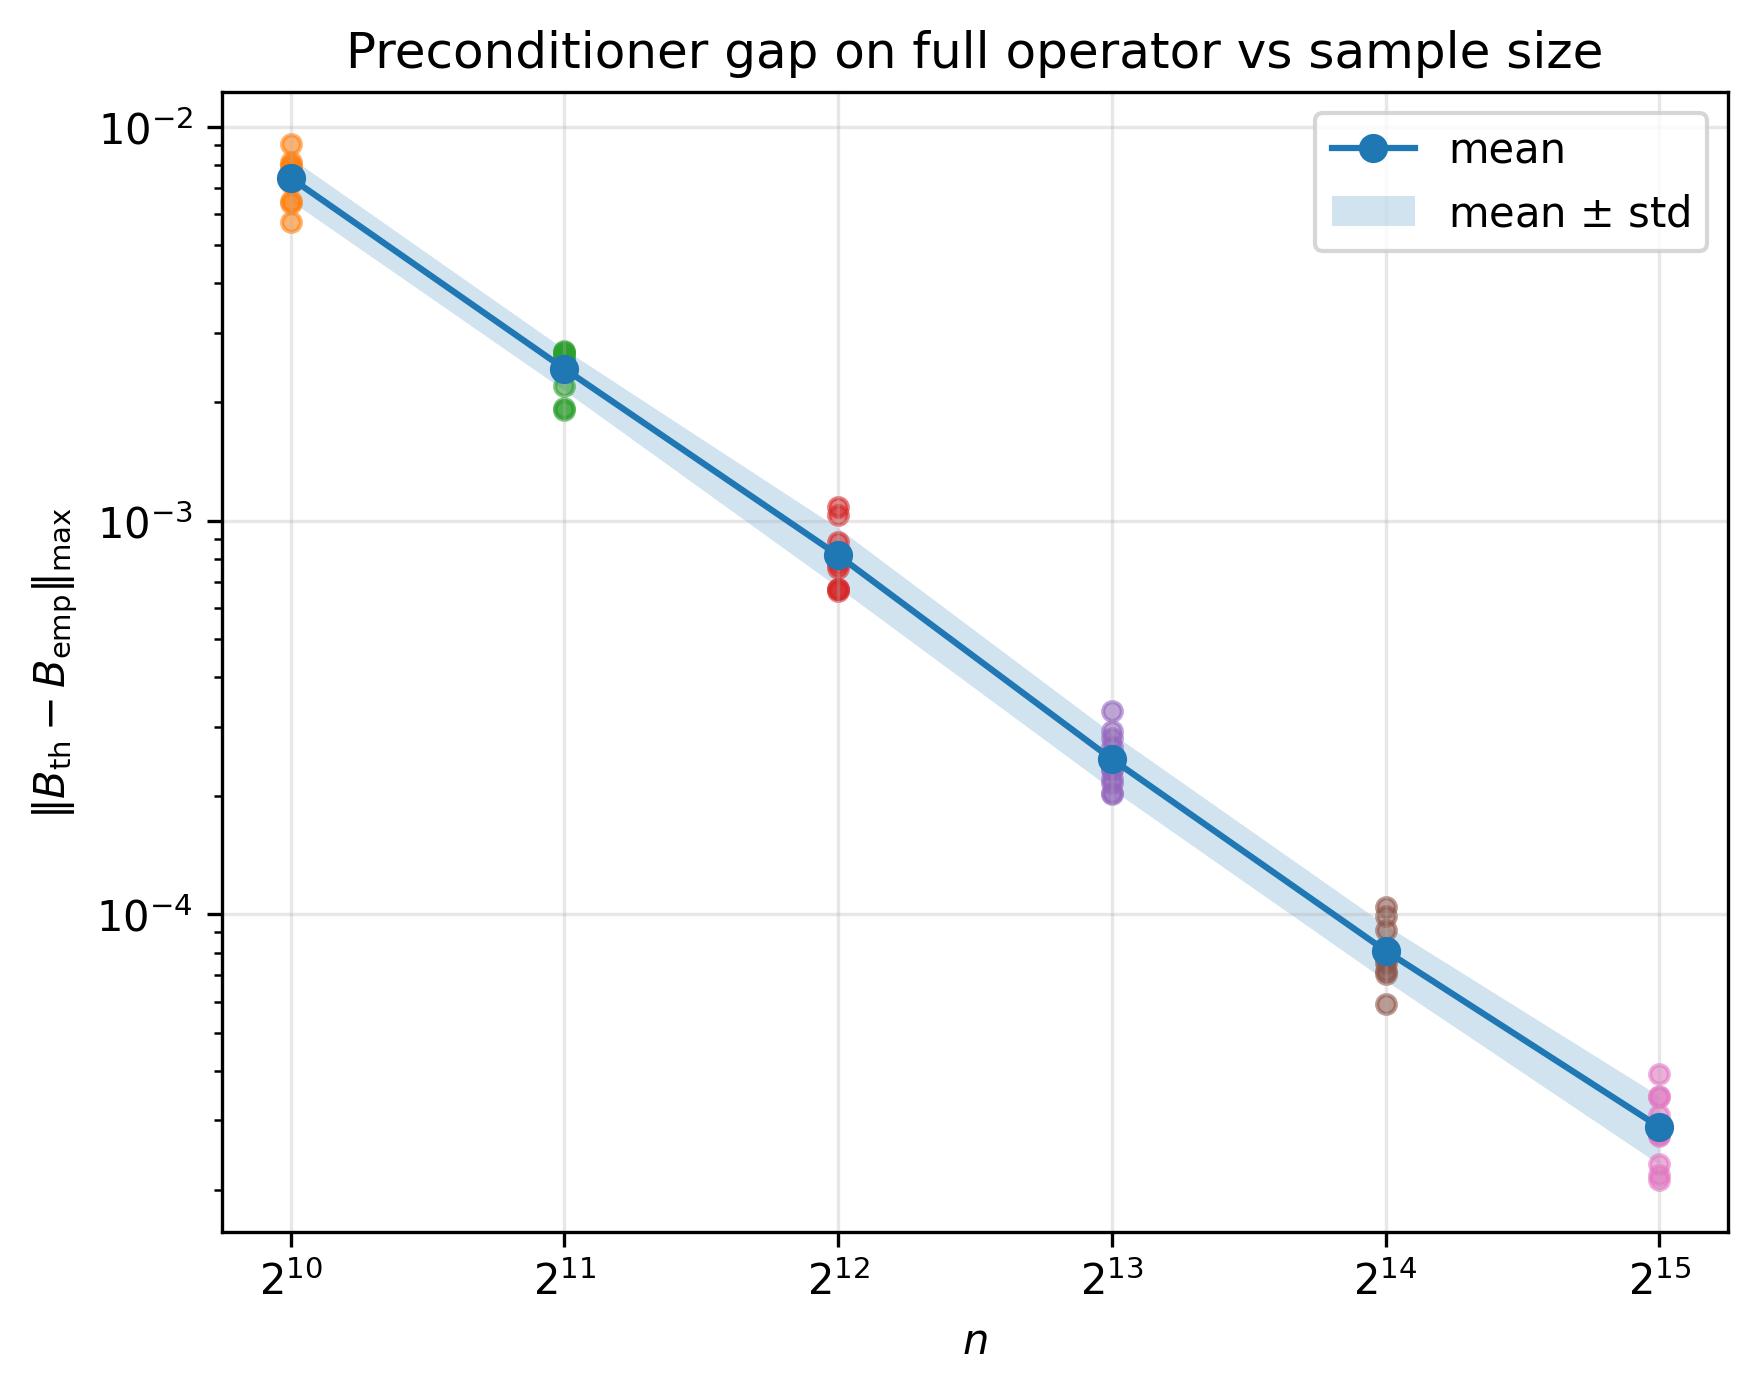
\includegraphics[width=\textwidth]{images/finite_sample_results/precond_diagnostic_B_th_vs_emp_max.png}
		\caption{\(\|B_{\mathrm{th}}-B_{\mathrm{emp}}\|_{\max}\)}
	\end{subfigure}
	\hfill
	\begin{subfigure}[t]{0.48\textwidth}
		\centering
		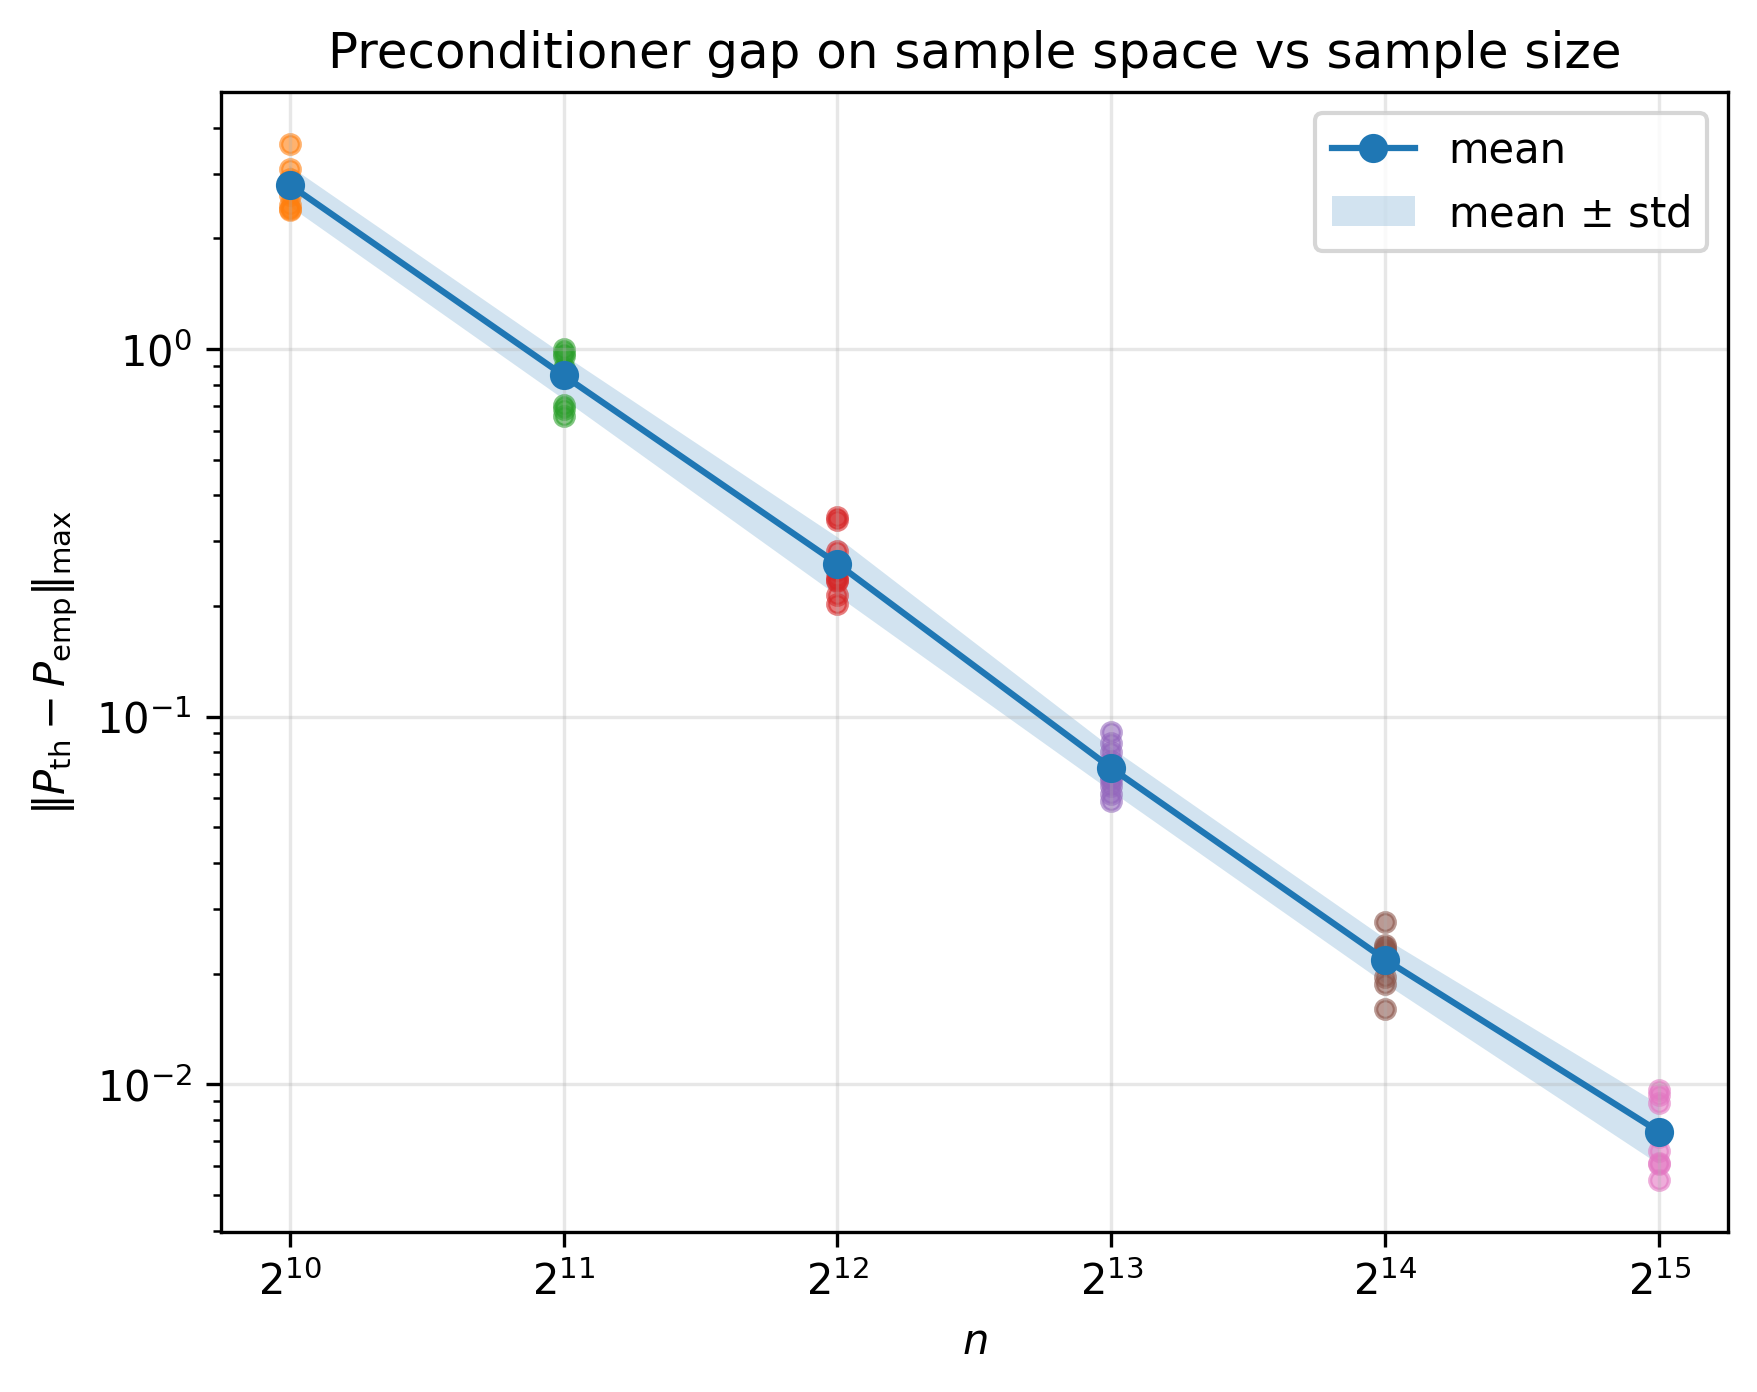
\includegraphics[width=\textwidth]{images/finite_sample_results/precond_diagnostic_P_th_vs_emp_max.png}
		\caption{\(\|P_{\mathrm{th}}-P_{\mathrm{emp}}\|_{\max}\)}
	\end{subfigure}

	\caption{Gap between the theory and empirical preconditioners as sample size
	increases. The empirical preconditioner uses the observed block \(C=G^{-1}H\),
	while the theory preconditioner uses the diagonal approximation
	\(\Lambda^{(n)}\). The decreasing gap is consistent with the finite-sample
	result \(C\approx\Lambda^{(n)}\).}
	\label{fig:results-preconditioner-gap}
\end{figure}

The preconditioning experiment gives a second test of the finite-sample
interpretation. The theory preconditioner uses only the predicted diagonal block
\(\Lambda^{(n)}\), while the empirical preconditioner uses the observed block
\(C_n^{(K)}=G^{-1}H\). If most of the rate separation is caused by the Fourier
eigenvalues, then rescaling by \(\Lambda^{(n)}\) should already make the
retained modes decay on more similar time scales. If the remaining
finite-sample mixing inside the retained block is important, then the empirical
preconditioner should give a visibly different dynamics.

Figures~\ref{fig:results-preconditioned-mode-decay},
\ref{fig:results-theory-precond-spectrum}, and
\ref{fig:results-preconditioner-gap} show that the theory preconditioner already
removes most of the rate separation on the retained block. The empirical
preconditioner is closer to the ideal flattened dynamics because it also
corrects the sample-dependent mixing in \(C_n^{(K)}\). The decreasing gap
between the two preconditioners as \(n\) increases is consistent with the
finite-sample result \(C_n^{(K)}\approx \Lambda^{(n)}\).

\subsection{Conditioning and the numerical floor}
\label{subsec:results-preconditioned-conditioning}

The preconditioned curves flatten at a level set by the numerical conditioning of
the problem. The condition number \(\kappa\) of a matrix measures how much it
amplifies relative errors when used to solve a linear system: a large \(\kappa\)
means small input errors can produce large errors in the solution, while
\(\kappa\) close to \(1\) means errors are barely amplified. The relevant matrix
here is the retained Fourier block. Before preconditioning this is \(C=G^{-1}H\),
the block whose deviation from \(\Lambda^{(n)}\) we have been tracking; after the
theory preconditioner it becomes \(C_{\mathrm{th}}=(\Lambda^{(n)})^{-1}C\), which
the preconditioner aims to bring close to the identity.

Table~\ref{tab:results-conditioning} reports both. The uncorrected block \(C\)
has condition number around \(330\) across sample sizes. This stays roughly
constant because it reflects the conditioning of the continuum block that \(C\)
converges to, set largely by the spread of the retained eigenvalues
\(\lambda_0,\dots,\lambda_K\), the largest of which is a few hundred times the
smallest. This spread does not depend on \(n\), so only the small finite-sample
correction makes \(\kappa(C)\) drift slightly as \(n\) grows. After the theory
preconditioner, \(\kappa(C_{\mathrm{th}})\) drops toward \(1\) as \(n\) grows,
which is the conditioning counterpart of \(C_n^{(K)}\to\Lambda^{(n)}\): as the
sampled block approaches the diagonal prediction, applying the inverse of that
diagonal prediction leaves an operator close to the identity. We omit the
empirical preconditioner, since it inverts the block exactly,
\(C_{\mathrm{emp}}^{-1}C=I_d\), giving \(\kappa=1\) by construction.

\begin{table}[!htbp]
	\centering
	\caption{Conditioning of the retained Fourier block and the resulting
		finite-precision floors, over \(10\) runs. \(\kappa(C)\) is the condition
		number of the uncorrected sampled block, \(\kappa(C_{\mathrm{th}})\) the
		condition number after the theory preconditioner is applied.
		The last two columns give the relative-accuracy floor
		\(\kappa u\), the condition number times the unit roundoff \(u\), at single
		and double precision.}
	\label{tab:results-conditioning}
	\begin{tabular}{rrrrr}
		\toprule
		\(n\)               & \(\kappa(C)\)       & \(\kappa(C_{\mathrm{th}})\) &
		\(\kappa u\) (fp32) & \(\kappa u\) (fp64)                                                                              \\
		\midrule
		1024                & 340.8               & 2.273                       & \(2.7\times10^{-7}\) & \(5.0\times10^{-16}\) \\
		2048                & 333.4               & 1.644                       & \(1.9\times10^{-7}\) & \(3.6\times10^{-16}\) \\
		4096                & 329.5               & 1.364                       & \(1.6\times10^{-7}\) & \(3.0\times10^{-16}\) \\
		8192                & 328.6               & 1.220                       & \(1.4\times10^{-7}\) & \(2.7\times10^{-16}\) \\
		16384               & 327.1               & 1.142                       & \(1.4\times10^{-7}\) & \(2.5\times10^{-16}\) \\
		32768               & 325.7               & 1.099                       & \(1.3\times10^{-7}\) & \(2.4\times10^{-16}\) \\
		\bottomrule
	\end{tabular}
\end{table}

Why conditioning sets the floor is visible in
Figure~\ref{fig:results-precision-comparison}, which repeats the experiment in
single and double precision. In finite-precision arithmetic, every operation
introduces a relative error of size \(u\), the unit roundoff (\(u\approx10^{-7}\)
in single precision, \(10^{-16}\) in double). Solving with a matrix of condition
number \(\kappa\) amplifies these errors, so the relative accuracy of the result
cannot be driven below about \(\kappa u\) \citep{trefethen2022numerical}. Because
the theory preconditioner makes \(\kappa(C_{\mathrm{th}})\) close to \(1\), this
floor is essentially \(u\) itself, and the curves plateau there. Moving from fp32
to fp64 lowers \(u\) by nine orders of magnitude and lowers the plateaus
correspondingly, which confirms the floor is numerical.

\begin{figure}[!htbp]
	\centering
	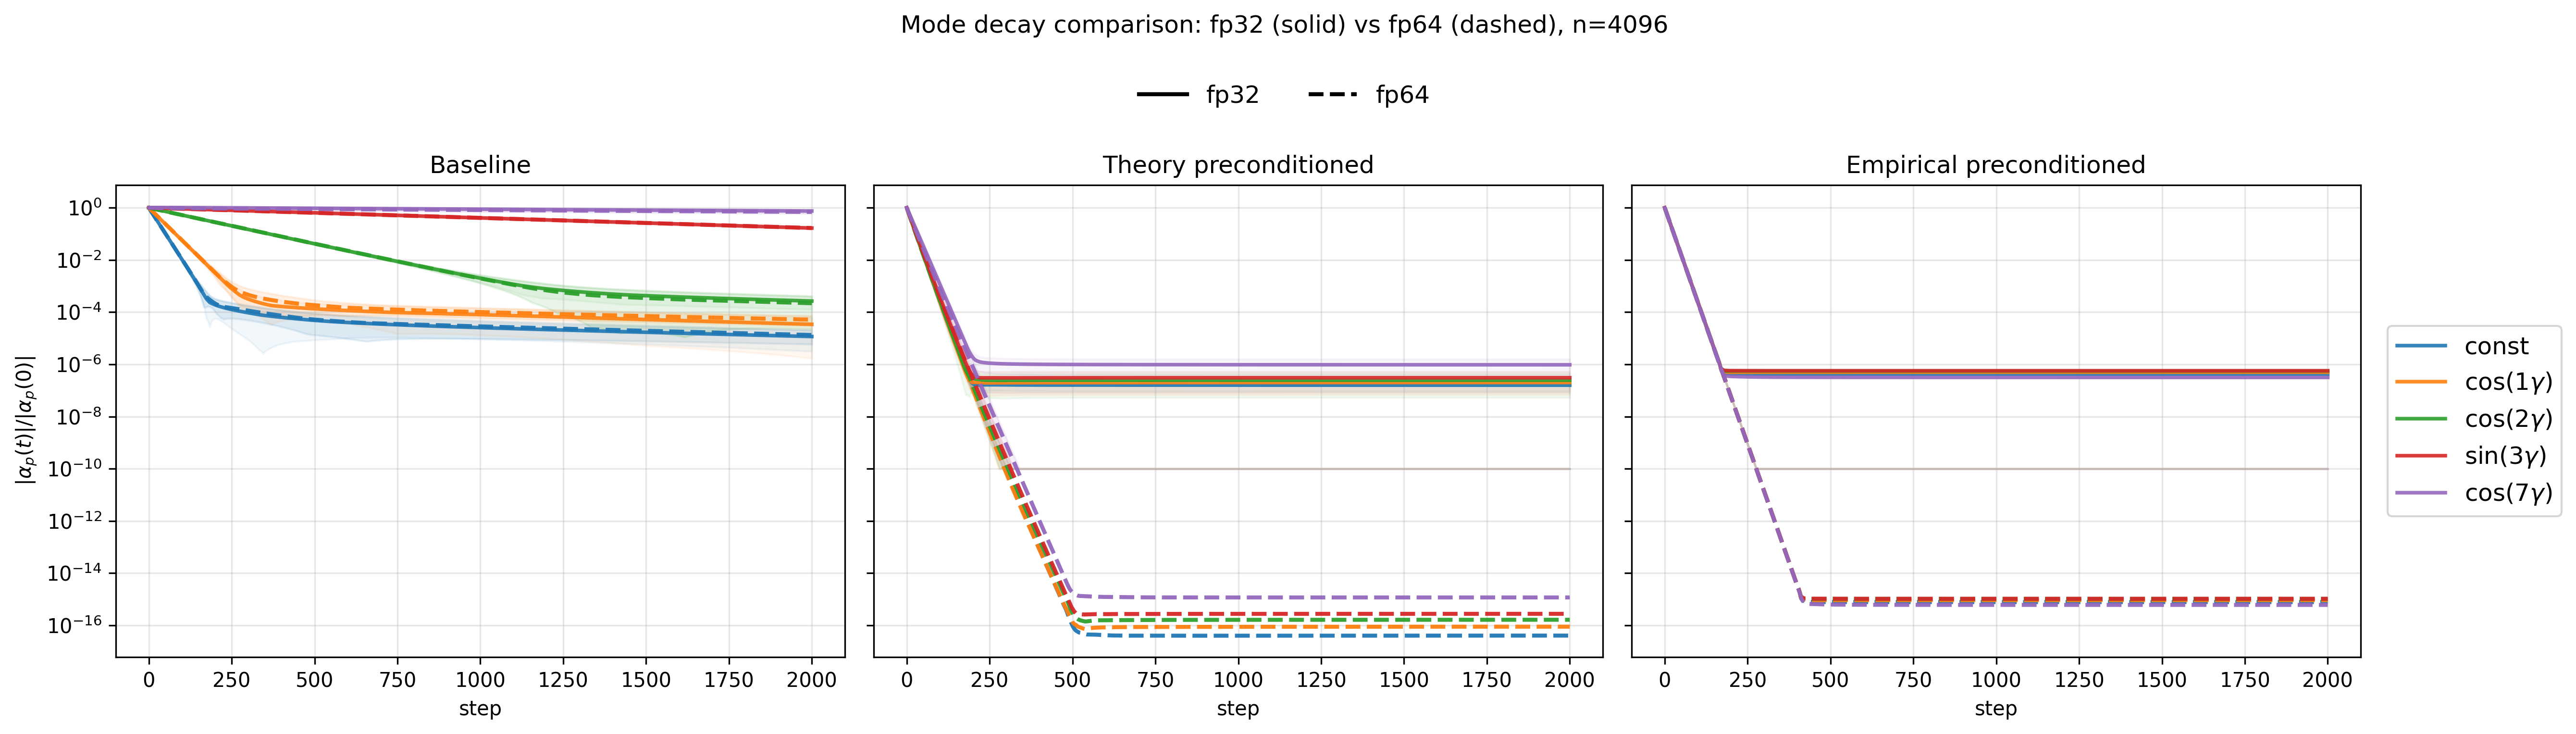
\includegraphics[width=\textwidth]{images/finite_sample_results/mode_decay_fp32_vs_fp64_three_panel_mean_std_n4096.png}
	\caption{Mode decay at \(n=4096\) in single (solid) and double (dashed)
		precision, for the baseline, theory-preconditioned, and empirically
		preconditioned dynamics. The preconditioned plateaus drop by several orders of
		magnitude from fp32 to fp64, identifying them as a finite-precision floor.}
	\label{fig:results-precision-comparison}
\end{figure}

\subsection{Targets with out-of-block frequencies}
\label{subsec:results-preconditioned-out-of-block}

The experiments so far kept all active target frequencies inside the retained
block. Figure~\ref{fig:results-precond-out-of-block} repeats the comparison with
a target that also contains frequencies outside the block, \(\sin(10\gamma)\) and
\(\cos(12\gamma)\). The preconditioner is still built only on the retained block,
so it accelerates the in-block modes as before but leaves the out-of-block modes
near their initial amplitude.

The in-block modes also plateau higher than in
Figure~\ref{fig:results-preconditioned-mode-decay}. This floor is not numerical:
the single- and double-precision curves reach nearly the same plateaus, so
roundoff is ruled out. We expect the cause to be coupling from the out-of-block
components. The sampled Fourier modes are only approximate eigenvectors of the
sampled operator, so the uncorrected modes at \(k=10\) and \(k=12\) can feed back
into the retained coordinates, and the in-block residuals would then settle at a
level set by this coupling. We have not isolated this mechanism directly, but it
is consistent with the modes being only approximate eigenvectors and with the
precision comparison ruling out roundoff.

\begin{figure}[!htbp]
	\centering
	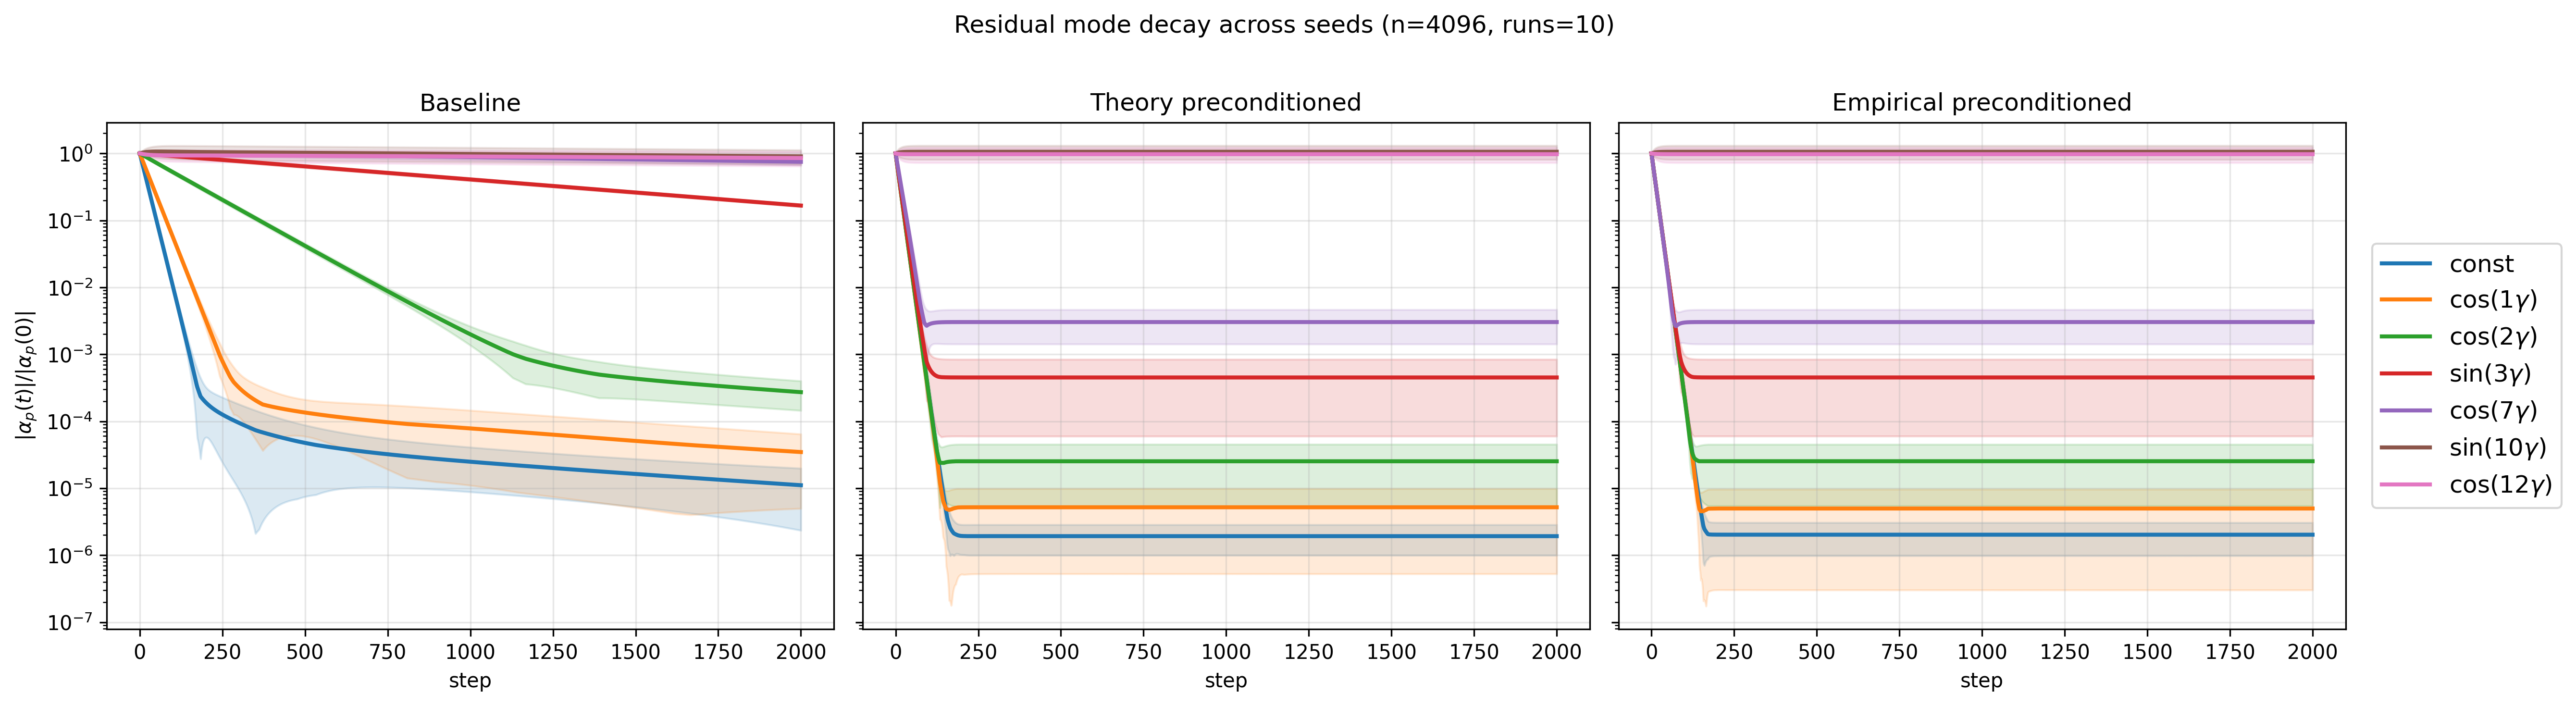
\includegraphics[width=\textwidth]{images/finite_sample_results/out_of_block_all_mode_decay_three_panel_mean_std_n4096.png}
	\caption{Preconditioned sampled dynamics with target frequencies outside the
		retained block, \(\sin(10\gamma)\) and \(\cos(12\gamma)\), at \(n=4096\) over
		\(10\) runs. The preconditioner accelerates the in-block modes but leaves the
		out-of-block modes near their initial amplitude. The in-block plateaus are
		higher than when all target modes lie inside the block, reflecting coupling
		from the uncorrected out-of-block components.}
	\label{fig:results-precond-out-of-block}
\end{figure}

\subsection{Discussion}
\label{subsec:results-preconditioned-discussion}

The preconditioning results connect to existing work on modifying NTK training
dynamics by changing the effective kernel spectrum. In particular,
\citet{geifman2024controlling} use preconditioned gradient descent to alter the
trajectory of wide-network training by modifying the spectrum of the associated
kernel. Recent work also studies preconditioned methods as a way to reduce
spectral bias and accelerate exploration of the NTK space
\citep{jiang2026convergencepreconditioned, yang2024sharpgeneralization}. Our
setting is more limited, since the preconditioner acts only on a fixed retained
Fourier block. The advantage is that the effect is explicit: rescaling by the
predicted eigenvalues directly compensates for the different decay rates of the
retained modes.

A practical use of this observation is as a block-level correction when the
target is known, or assumed, to be concentrated on a prescribed low-frequency
Fourier range. In that case, the theory preconditioner does not require
estimating the full sampled block inverse. It only uses the predicted
finite-sample eigenvalues \(\lambda_p^{(n)}\), and can make the retained
components converge on more similar time scales. The empirical preconditioner
gives the best correction when the sampled block is available, while the theory
preconditioner provides a cheaper approximation whose accuracy improves as the
finite-sample Fourier block becomes closer to diagonal.

Overall, the finite-sample results show that random sampling turns the exact
continuum Fourier dynamics into an approximate low-frequency description. The
sampled operator is no longer exactly diagonal in the Fourier basis, but its
deviation from the corrected diagonal prediction decreases with \(n\) and
explains the observed residual dynamics.

So far, however, the kernel itself has still been the deterministic
infinite-width NTK. In an actual finite-width network, the tangent kernel at
initialization is built from randomly initialized weights, so even before
training it is a random finite-width approximation of the continuum kernel. The
next section therefore asks whether the same Fourier structure survives this
second perturbation: finite width.

\section{Finite-width control of the frozen tangent operator}
\label{sec:results-finite-width-frozen}

We now turn from sampling error to width-induced error. Throughout this section, the input
space remains the continuum \(S^1\), and the object of interest is the frozen finite-width
operator \(B_m^{(K)}\) on the truncated Fourier subspace \(\mathcal H_K\), introduced in
\eqref{eq:method-finite-width-block}. The corresponding continuum reference block
\(\Lambda_K\) was defined in \eqref{eq:method-continuum-fourier-block}.

The next theorem shows that, for each fixed \(K\), the frozen finite-width block is a
controlled perturbation of the continuum Fourier block.

\begin{theorem}[Finite-width concentration of the frozen low-mode operator]
	\label{thm:results-finite-width-frozen-concentration}
	Fix \(K\ge 1\), and let \(d=2K+1\). Then
	\begin{equation}
		\mathbb E[B_m^{(K)}]=\Lambda_K.
		\label{eq:results-finite-width-mean}
	\end{equation}
	Moreover, there exists a universal constant \(c>0\) such that, for every
	\(\varepsilon>0\),
	\begin{equation}
		\mathbb P\!\left(
		\|B_m^{(K)}-\Lambda_K\|_{\max}\ge \varepsilon
		\right)
		\le
		2d^2
		\exp\!\left(
		-cm\min\!\left(\frac{\varepsilon^2}{32^2},\frac{\varepsilon}{32}\right)
		\right).
		\label{eq:results-finite-width-max-bound}
	\end{equation}
	Equivalently, for every \(\delta\in(0,1)\), with probability at least
	\(1-\delta\),
	\begin{equation}
		\|B_m^{(K)}-\Lambda_K\|_{\max}
		\le
		32\max\left\{
		\sqrt{\frac{1}{cm}\log\!\left(\frac{2d^2}{\delta}\right)},
		\frac{1}{cm}\log\!\left(\frac{2d^2}{\delta}\right)
		\right\}.
		\label{eq:results-finite-width-high-prob-bound}
	\end{equation}
	In particular, for fixed \(K\),
	\begin{equation}
		\|B_m^{(K)}-\Lambda_K\|_{\max}
		=
		O \!\left(\sqrt{\frac{\log K}{m}}\right).
		\label{eq:results-finite-width-rate}
	\end{equation}
\end{theorem}

The detailed proof is provided in Appendix~\ref{app:finite-width-frozen-proofs}.

Theorem~\ref{thm:results-finite-width-frozen-concentration} shows that, on a
fixed truncated Fourier subspace, the frozen finite-width tangent block is a
random perturbation of the continuum Fourier block. The perturbation decreases
with width at the usual \(m^{-1/2}\) concentration scale, up to logarithmic
factors in the block dimension. However, the theorem contains an unspecified
universal constant \(c>0\). This constant comes from Bernstein's inequality for
averages of centered sub-exponential random variables
\citep{Vershynin_2018a}. In explicit proofs of such inequalities, constants of
order \(1/4\) often appear after converting a \(\psi_1\)-norm bound into a
moment generating function bound. We next check this concentration behavior numerically where
we use \(c=0.2\) as a conservative
representative value, not an optimized constant for this problem. Changing this
constant shifts the bound but does not change the predicted rate as \(m\) increases.

For each width \(m\), we sample 100 independent initializations and compute
\[
	\|B_m^{(K)}-\Lambda_K\|_{\max}.
\]
Figure~\ref{fig:results-finite-width-concentration} shows the median and
\(95\%\) quantile of this error, together with the rate envelope suggested by
Theorem~\ref{thm:results-finite-width-frozen-concentration}.
The empirical errors decrease steadily with width. The theoretical envelope is
much larger than the observed errors, but it has the correct qualitative trend:
the finite-width block concentrates around the continuum Fourier block as \(m\)
increases.

\begin{figure}[!htbp]
	\centering
	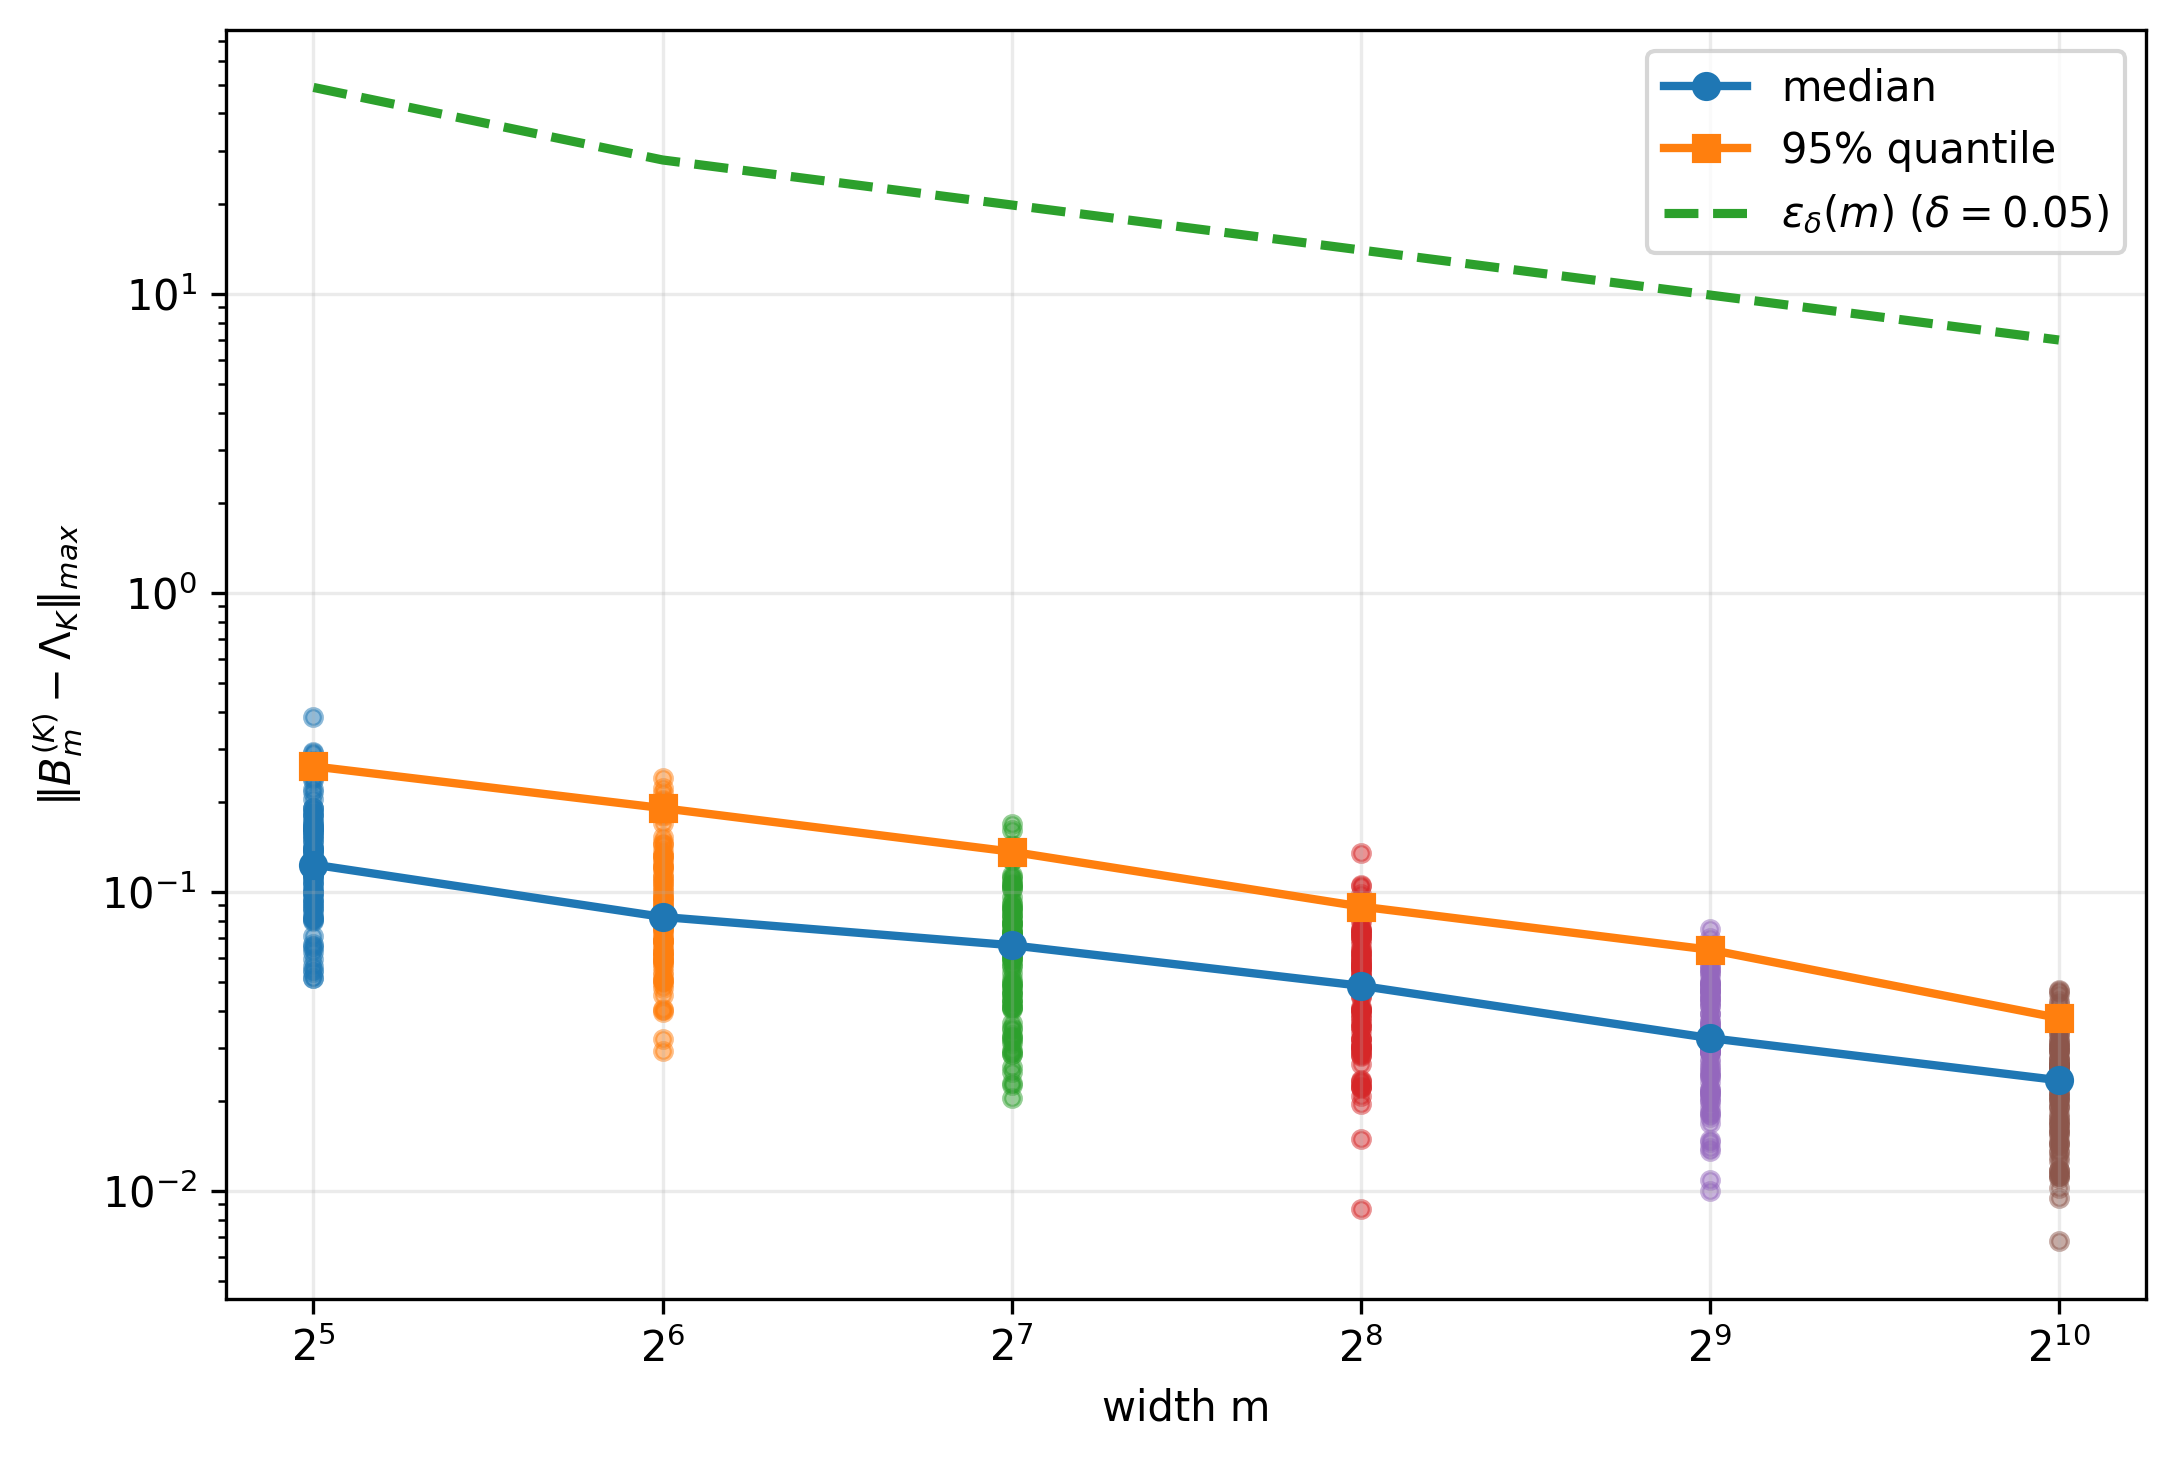
\includegraphics[width=0.82\textwidth]{images/finite_width_results/03_concentration_B_m.png}
	\caption{Finite-width concentration of the frozen tangent block. For each
	width \(m\), the plot shows the median and \(95\%\) quantile of
	\(\|B_m^{(K)}-\Lambda_K\|_{\max}\) across 100 independent initializations. The
	dashed curve shows the rate envelope from
	Theorem~\ref{thm:results-finite-width-frozen-concentration} with
	\(\delta=0.05\) and the illustrative constant \(c=0.2\). The empirical errors
	decrease with width, while the explicit envelope is conservative.}
	\label{fig:results-finite-width-concentration}
\end{figure}

This is the finite-width analogue of the finite-sample
control from the previous section. In the finite-sample case, the randomness
comes from replacing the uniform measure by sampled points. Here, the randomness
comes from the finite number of hidden units at initialization. In both cases,
on a fixed low-frequency Fourier block, the
operator remains close to the deterministic continuum Fourier block, and the
deviation decreases as the relevant size parameter (number of samples or width of network) increases.

Thus finite width alone does not destroy the Fourier structure of the frozen
tangent operator. For a particular random initialization, the operator is not
exactly diagonal in the Fourier basis, but
Theorem~\ref{thm:results-finite-width-frozen-concentration} and
Figure~\ref{fig:results-finite-width-concentration} show that this mismatch
shrinks with width. This supports the use of the infinite-width NTK as a
baseline, while also showing why finite-width fluctuations can matter
quantitatively
\citep{jacot2018ntk,lee2020wide,bordelon2023dynamicsfinitewidthkernel,
	vyas2022limitationsntkunderstandinggeneralization}.

The next question is whether this entrywise concentration also corresponds to
geometric agreement of the frequency subspaces themselves.

\subsection{Empirical alignment of Fourier frequency subspaces}
\label{subsec:results-finite-width-subspace-alignment}

The block concentration result controls the matrix \(B_m^{(K)}\) on the retained
Fourier coordinates. We next examine the corresponding eigenspaces directly.
Using the quantities introduced in
Section~\ref{subsec:method-projector-error}, we compare each Fourier frequency
subspace \(\mathcal F_k\) with a matched empirical eigenspace
\(\widehat{\mathcal F}_k\) of the frozen finite-width operator.

We first summarize the comparison using the projector error
\[
	\varepsilon_{k,F}^{(m)}
	=
	\|\widehat P_k-P_k\|_F .
\]
This gives one scalar mismatch measure for each frequency subspace. By
\eqref{eq:method-projector-angle-identity}, it is equivalent to combining the
principal angles between \(\mathcal F_k\) and \(\widehat{\mathcal F}_k\).

Figure~\ref{fig:results-finite-width-projector-error} shows the mean and
standard deviation of \(\varepsilon_{k,F}\) across random initializations.
For all displayed frequencies, the projector error decreases as the width
increases. Higher frequencies generally have larger projector error at a fixed
width. One exception in this experiment is \(k=2\), which has the smallest
projector error among the displayed frequencies.
A plausible explanation is the structural role of
\(k=0\) and \(k=1\) in this chosen architecture.
The constant mode receives a direct eigenvalue contribution from the trainable
hidden-bias term (refer Theorem~\ref{thm:results-continuum-spectrum}).
The first frequency, \(k=1\), is tied to the coordinate embedding,
\[
	x(\varphi)=(\cos\varphi,\sin\varphi)
\]
and it is also the only odd frequency
present in the no-bias kernel (Corollary~\ref{cor:results-bias-spectrum}), with

\[
	\lambda_1^{(\mathrm{nb})}=\frac14,
	\qquad
	\lambda_k^{(\mathrm{nb})}=0
	\quad \text{for odd } k\ge 3.
\]
These features may make the finite-width perturbation act differently on \(k=0\) and \(k=1\) than on the
higher frequency blocks. We do not investigate this mechanism further here, so
the \(k=2\) behavior is an empirical observation and not a theoretical claim.

\begin{figure}[!htbp]
	\centering
	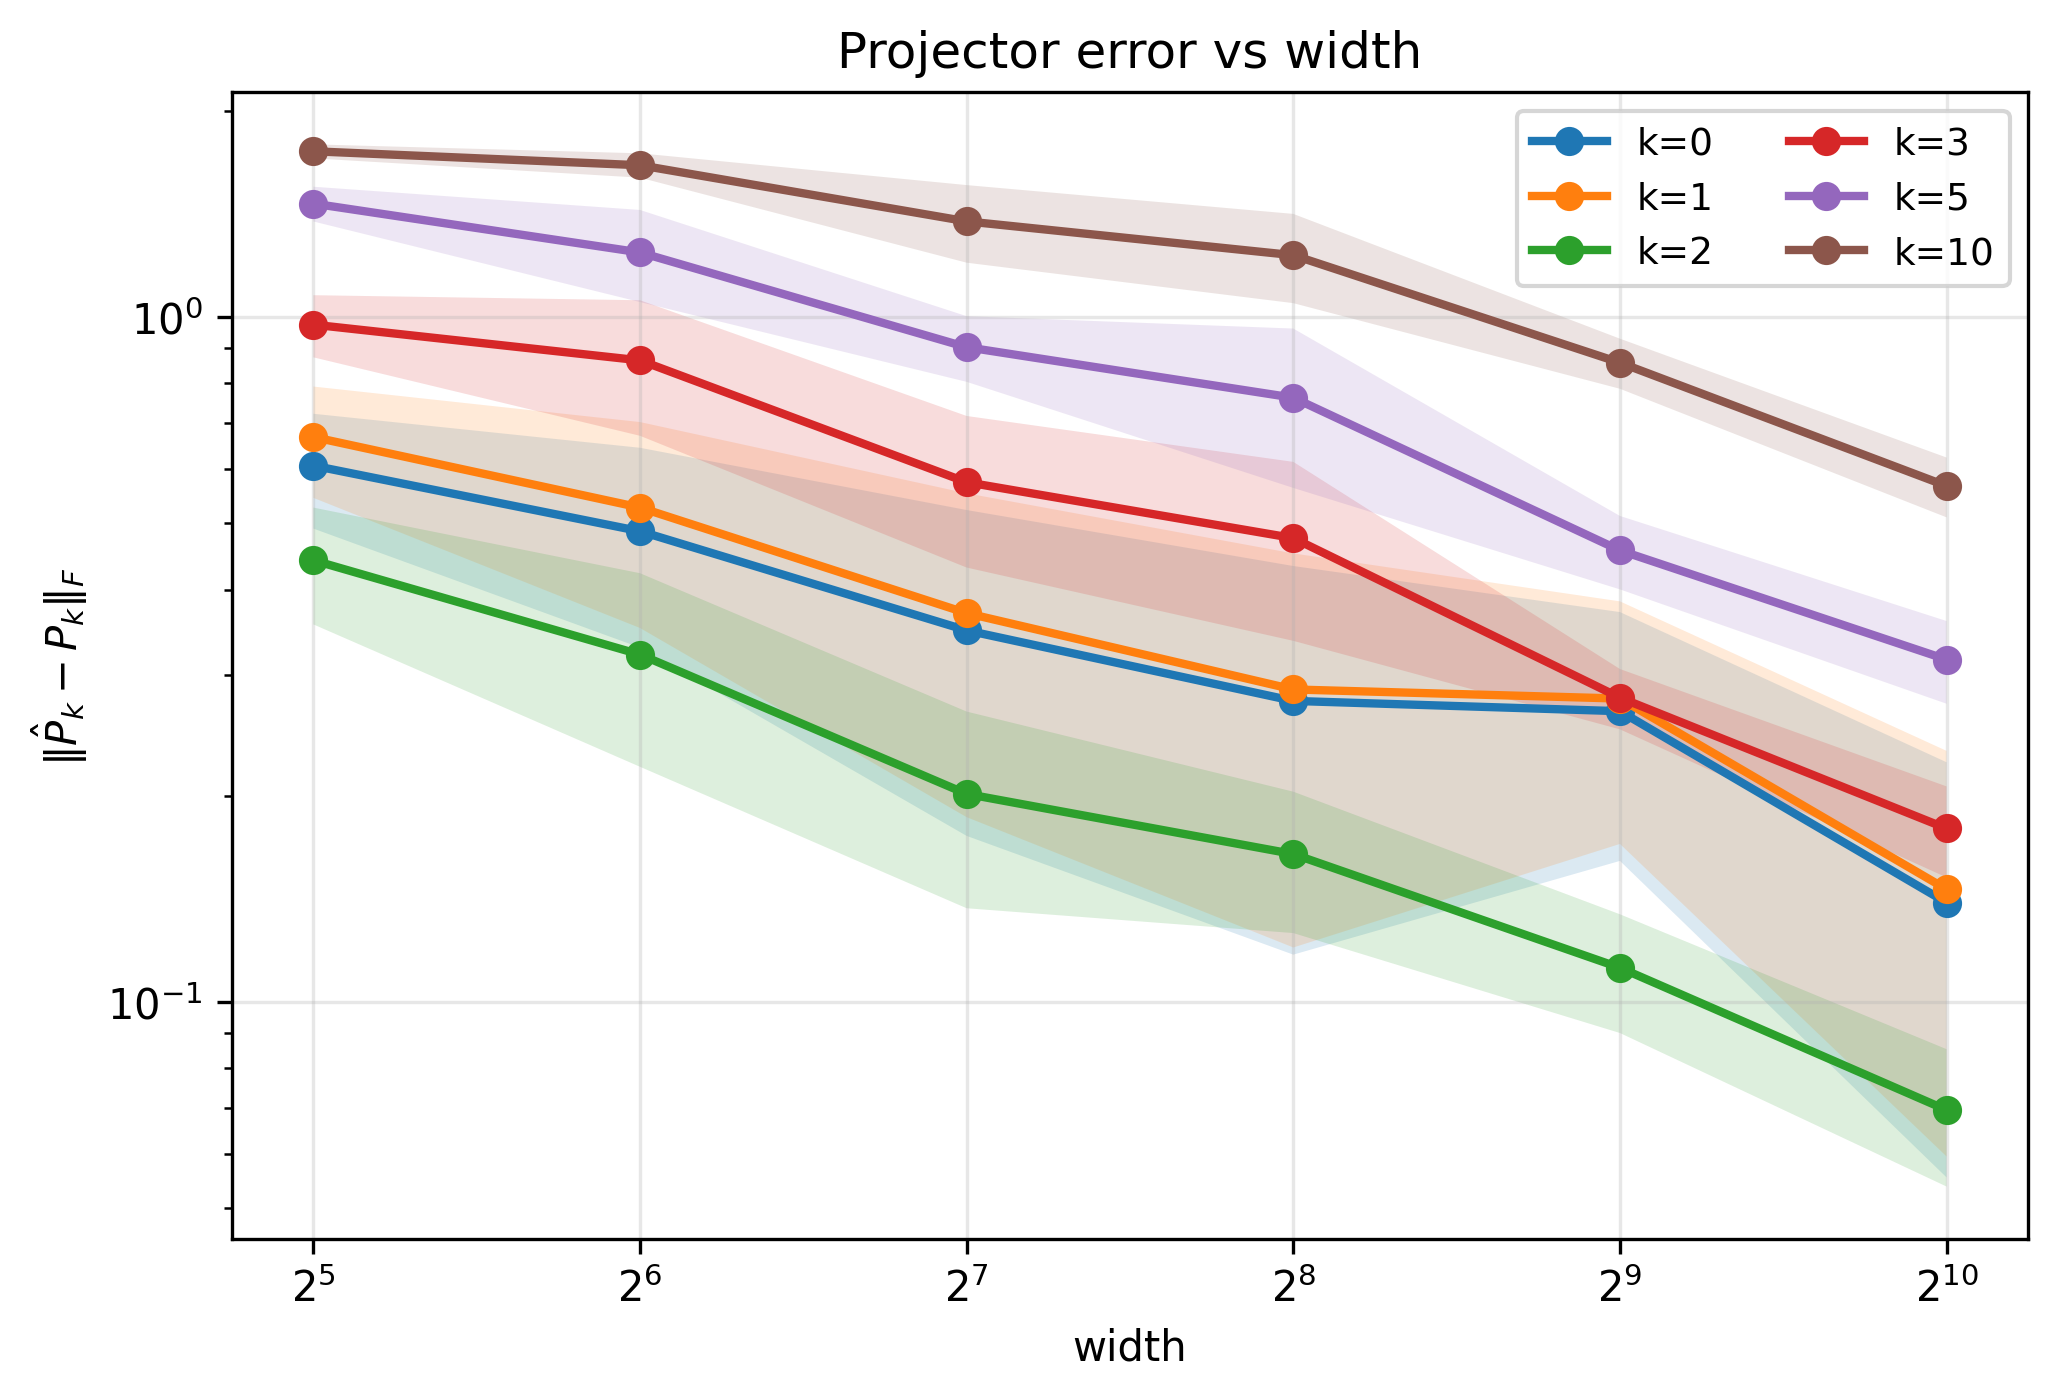
\includegraphics[width=0.78\textwidth]{images/finite_width_results/projector_error_vs_width.png}
	\caption{Projector error
		\(\|\widehat P_k-P_k\|_F\) between the Fourier frequency subspace
		\(\mathcal F_k\) and the matched empirical eigenspace
		\(\widehat{\mathcal F}_k\) of the frozen finite-width operator at
		initialization. The markers show the mean over random initializations and the
		shaded regions show one standard deviation. The error decreases with width
		for all displayed frequencies.}
	\label{fig:results-finite-width-projector-error}
\end{figure}

The projector error gives one scalar measure of subspace mismatch. As a
complementary summary, we also report the subspace cosine similarity defined in
\eqref{eq:method-subspace-cosine-similarity}. This quantity averages the
squared cosines of the principal angles between \(\mathcal F_k\) and
\(\widehat{\mathcal F}_k\), and lies between \(0\) and \(1\). Larger values
indicate better alignment, with value \(1\) corresponding to perfect agreement
of the two subspaces.

Figure~\ref{fig:results-finite-width-subspace-cosine-similarity} shows this
alignment score across widths. The alignment improves with \(m\) for all
displayed frequencies, matching the trend in the projector-error plot. Lower
frequencies are already well aligned at small width, while higher frequencies
require larger widths to approach the continuum Fourier subspaces. As before,
\(k=2\) is unusually well aligned compared with neighbouring displayed
frequencies.

% \begin{figure}[H]
% 	\centering
% 	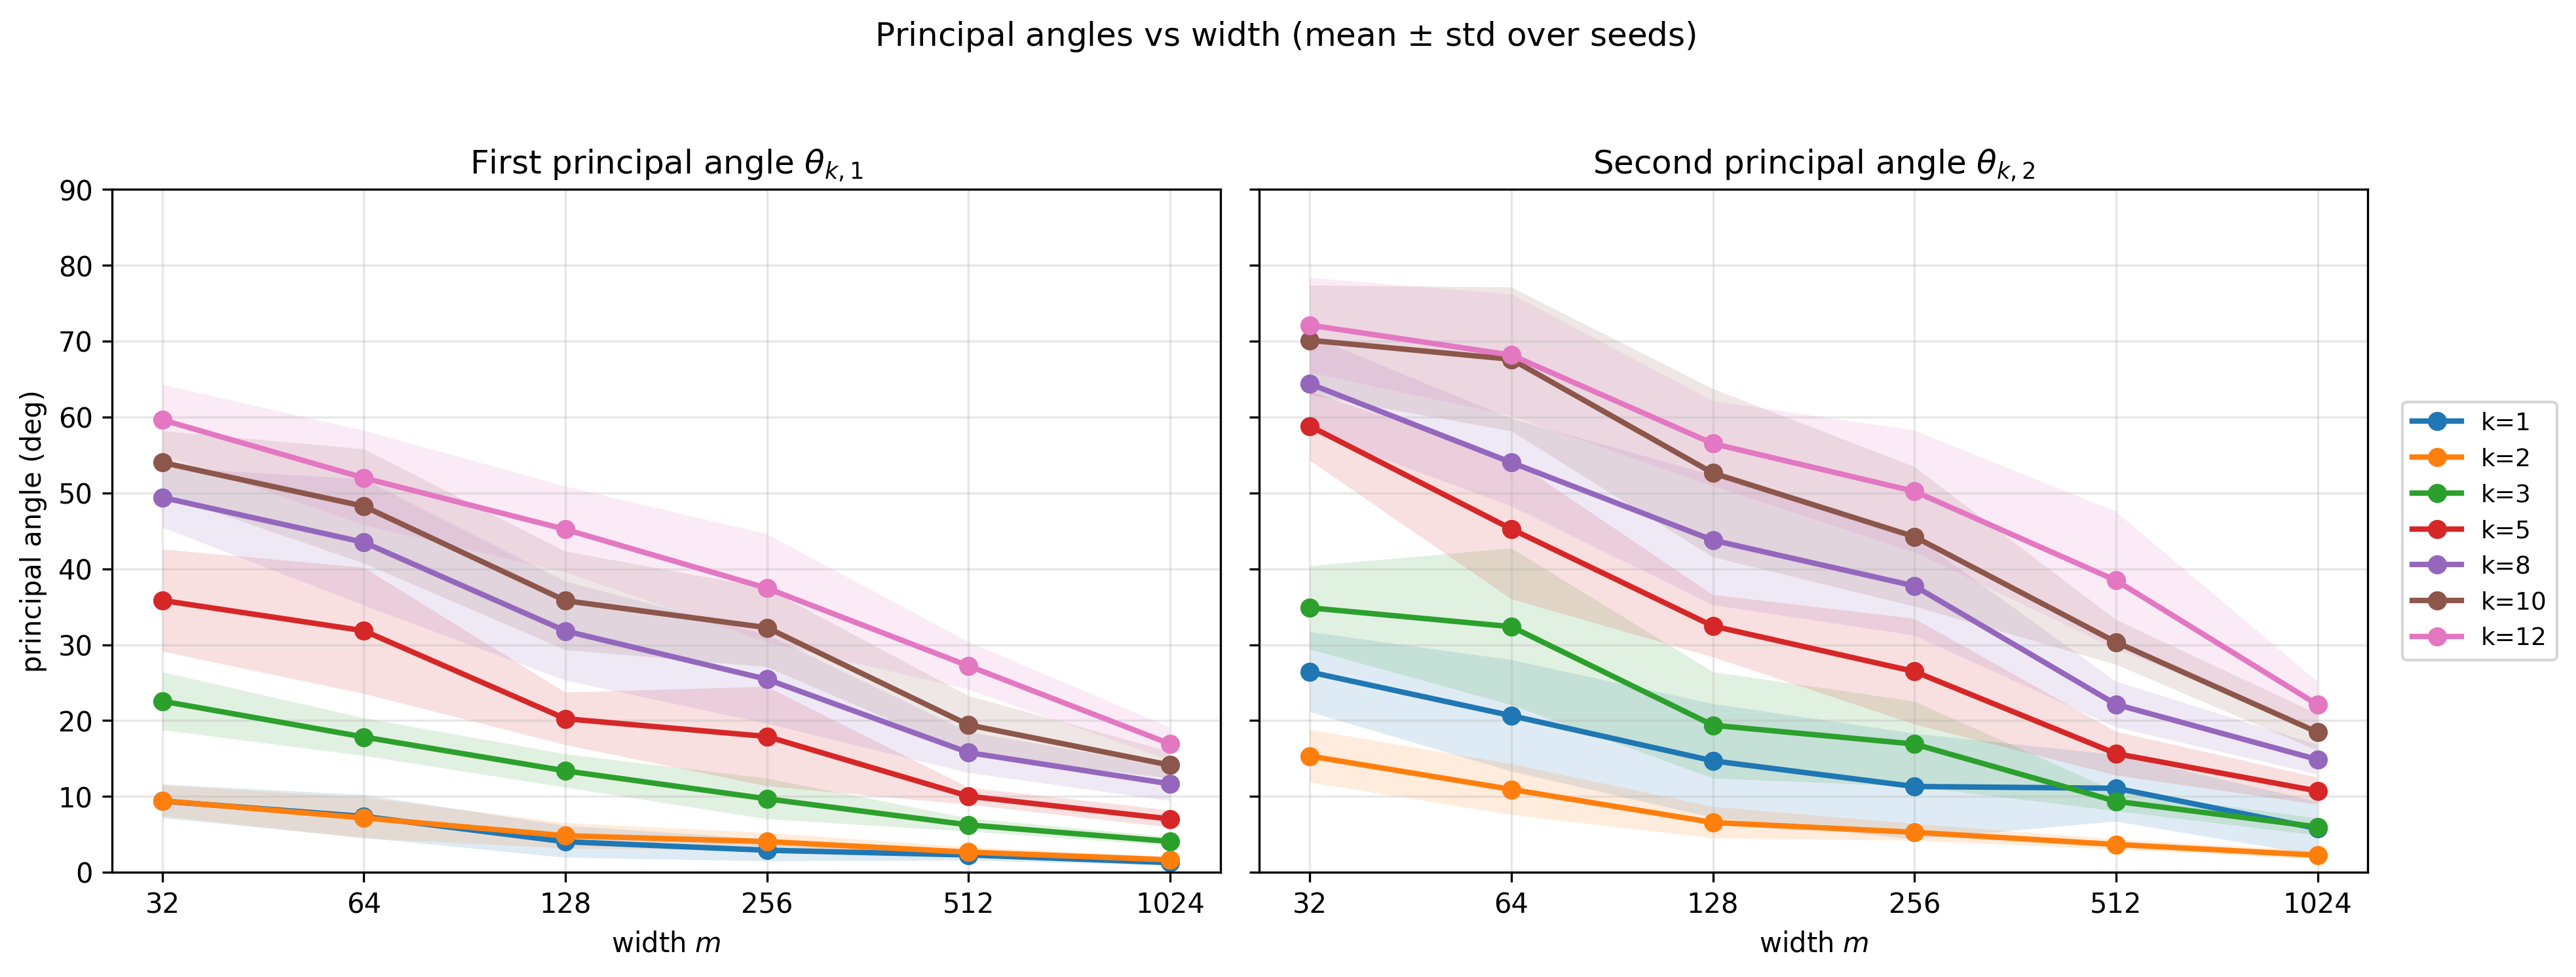
\includegraphics[width=\textwidth]{images/finite_width_results/principal_angles_vs_width.png}
% 	\caption{Principal angles between the Fourier frequency subspace
% 		\(\mathcal F_k\) and the matched empirical eigenspace
% 		\(\widehat{\mathcal F}_k\) of the frozen finite-width operator at
% 		initialization. The left panel shows the first principal angle
% 		\(\theta_{k,1}\), and the right panel shows the second principal angle
% 		\(\theta_{k,2}\). The markers show the mean over random initializations and
% 		the shaded regions show one standard deviation. The principal angles tend to
% 		decrease with width.}
% 	\label{fig:results-finite-width-principal-angles}
% \end{figure}

\begin{figure}[!htbp]
	\centering
	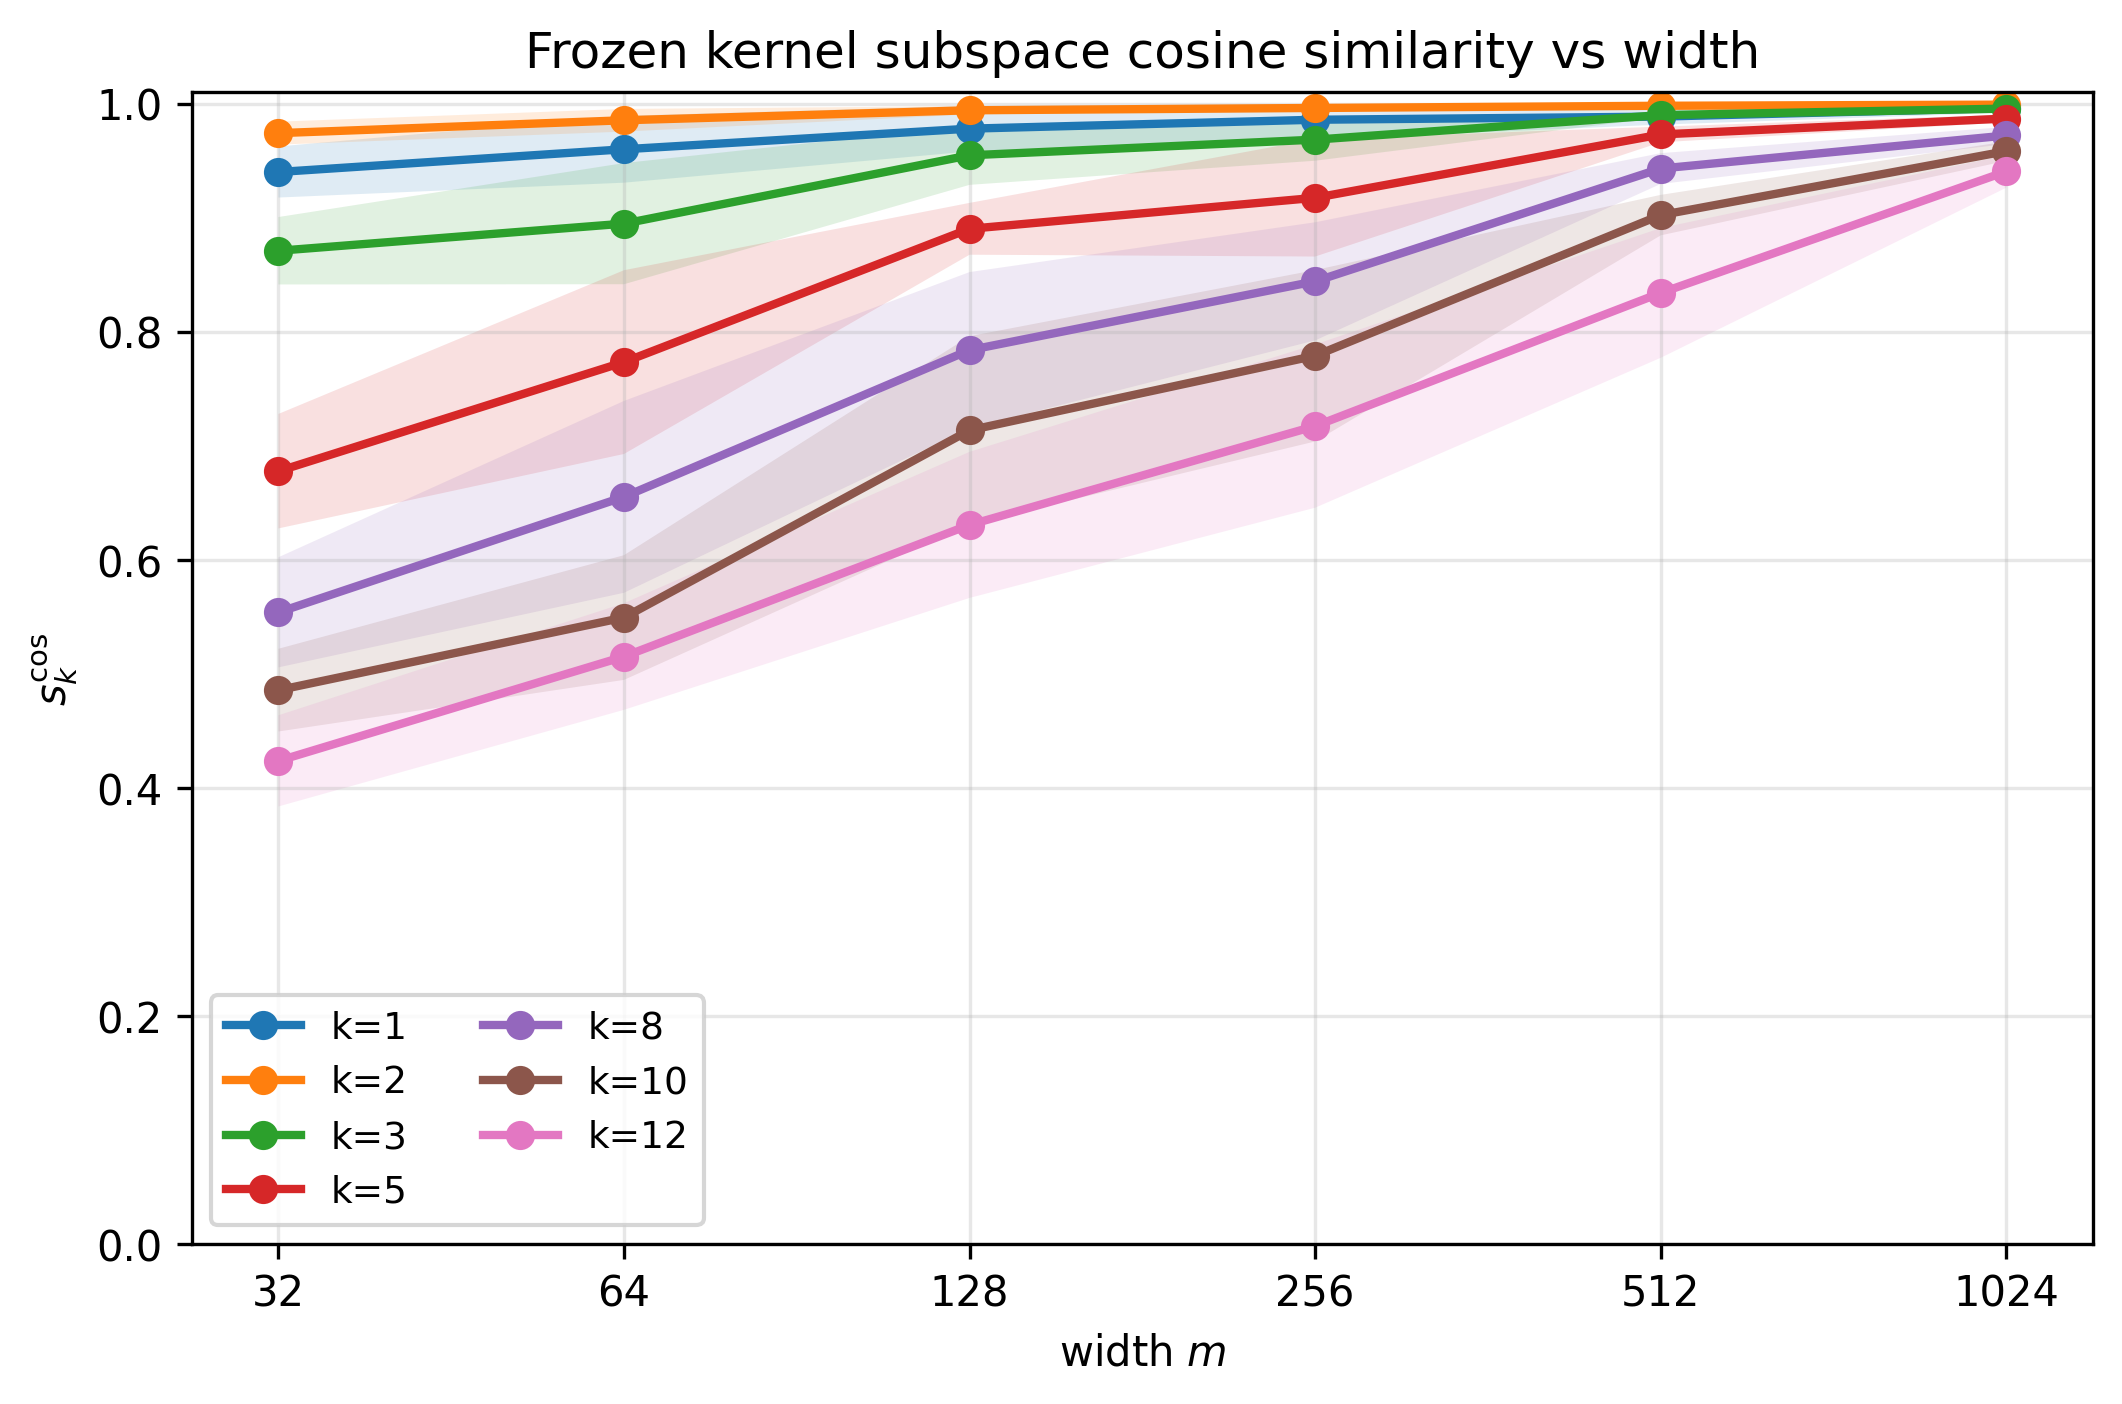
\includegraphics[width=0.78\textwidth]{images/finite_width_results/rms_cos_similarity_vs_width.png}
	\caption{Subspace cosine similarity between the Fourier frequency subspace
		\(\mathcal F_k\) and the matched empirical eigenspace
		\(\widehat{\mathcal F}_k\) of the frozen finite-width operator at
		initialization. The markers show the mean over random initializations and
		the shaded regions show one standard deviation. Larger values indicate
		better subspace alignment, with value \(1\) corresponding to perfect
		alignment. The alignment improves with width for all displayed frequencies,
		with higher frequencies requiring larger widths to approach the continuum
		Fourier subspaces.}
	\label{fig:results-finite-width-subspace-cosine-similarity}
\end{figure}

Taken together, Figures~\ref{fig:results-finite-width-concentration},
\ref{fig:results-finite-width-projector-error}, and
\ref{fig:results-finite-width-subspace-cosine-similarity} show the same finite-width
trend from complementary viewpoints. The matrix block \(B_m^{(K)}\) approaches
the continuum block \(\Lambda_K\) as \(m\) increases, and the matched empirical
eigenspaces become closer to the corresponding Fourier frequency subspaces.
The improvement is strongest at small and moderate widths for the higher
frequencies, which are the most poorly aligned at small width.

The concentration theorem controls the absolute error
\(|B_m^{(K)}-\Lambda_K|_{\max}\). To interpret its effect on a particular
Fourier component, this error should be compared with the size of the
corresponding continuum eigenvalue. In the continuum fixed-kernel model, mode
\(k\) decays at rate \(\lambda_k\), and
Theorem~\ref{thm:results-continuum-spectrum} gives
\[
	\lambda_k = O(k^{-2})
	\qquad (k\to\infty),
\]
for both even and odd frequencies. Thus, the same absolute perturbation is less
important for low-frequency modes with larger eigenvalues, and can be more
visible for high-frequency modes with smaller eigenvalues. This explains why the
finite-width perturbation is expected to matter more for higher frequencies.

Figures~\ref{fig:results-finite-width-subspace-cosine-similarity} and
\ref{fig:results-finite-width-projector-error}, support this interpretation
geometrically. For \(k \ge 1\), each Fourier frequency corresponds to a
two-dimensional plane spanned by the cosine and sine modes. At finite width,
the matched empirical eigenspace need not coincide exactly with this plane. The
projector-error and cosine-similarity plots show that this mismatch decreases
with width. They also show that the amount of alignment can vary substantially
across frequencies at the same width. One plausible explanation is that
eigenspace stability depends not only on the size of the finite-width
perturbation, but also on the local spectral separation of the corresponding
continuum eigenspace. Since higher-frequency eigenvalues are smaller and closer
together, their eigenspaces may be more sensitive to the same absolute
perturbation.

Overall, the frozen finite-width results show that finite width does not
destroy the Fourier structure at initialization. It introduces a random
perturbation of the continuum Fourier operator, and this perturbation decreases
with width. The result is, therefore, a frozen-kernel baseline: before training
changes the tangent operator, the continuum Fourier eigenspaces remain a useful
reference, but finite-width fluctuations can already affect higher-frequency
components more strongly. This is consistent with empirical observations that
higher-frequency components are learned later and are more sensitive to the
data distribution and to perturbations
\citep{rahaman2019spectralbiasneuralnetworks,basri2019convergence,basri2020frequencybiasneuralnetworks}.

The part not settled here is the evolving finite-width case. During training,
the tangent operator can change, so the frozen Fourier block structure need not
remain fixed. The finite-width result therefore gives us a
frozen-kernel baseline but not a complete theory of finite-width training
\citep{bordelon2023dynamicsfinitewidthkernel,vyas2022limitationsntkunderstandinggeneralization,golikov2022neuraltangentkernelsurvey}.

\section{Evolving finite-width tangent kernel}
\label{sec:results-evolving-kernel}

The previous section studied the frozen tangent operator at initialization. We
now compare this frozen baseline with the tangent operator that evolves during
training. Unlike the finite-width concentration result above, this part is
empirical. The goal is to understand how kernel evolution changes the Fourier
picture at finite width.

\subsection{Loss decay across widths}
\label{subsec:results-evolving-loss}

We first compare the least-squares objective under frozen and evolving
finite-width tangent-kernel dynamics across widths. The cross-width comparison
in Figure~\ref{fig:evolving-cross-width-loss} gives the overall trend, while
Figure~\ref{fig:evolving-loss-by-width} shows the width-by-width frozen versus
evolving comparison in more detail.

\begin{figure}[!htbp]
	\centering
	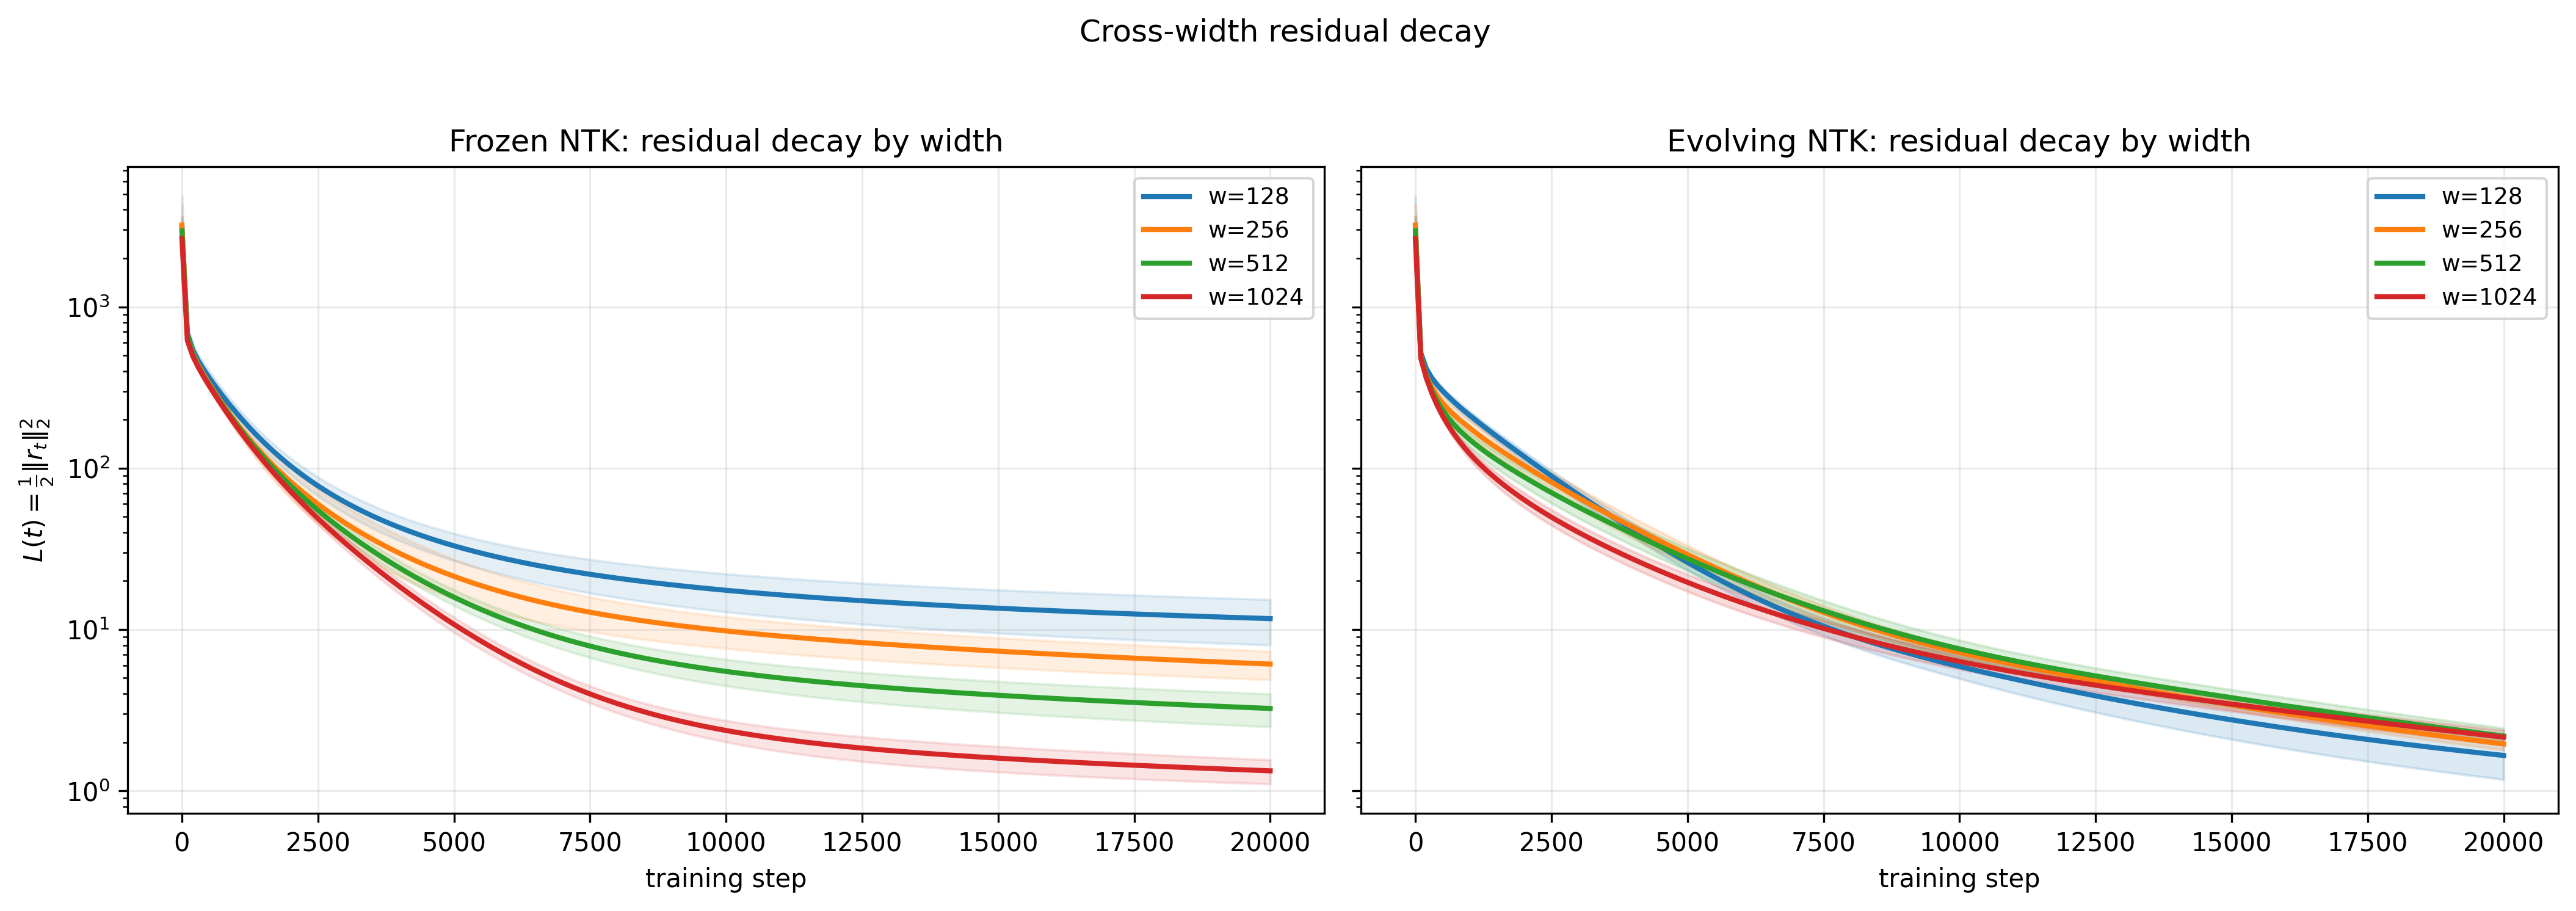
\includegraphics[width=0.95\textwidth]{images/finite_width_evolving_results/cross_width_residual_decay.png}
	\caption{Cross-width comparison of the least-squares objective
		\(L(t)=\frac{1}{2}\|r_t\|_2^2\) under frozen and evolving tangent-kernel
		dynamics. In the frozen regime, larger width gives consistently better
		residual decay. In the evolving regime, the curves are closer across widths.}
	\label{fig:evolving-cross-width-loss}
\end{figure}

\begin{figure}[!htbp]
	\centering
	\begin{subfigure}[t]{0.48\textwidth}
		\centering
		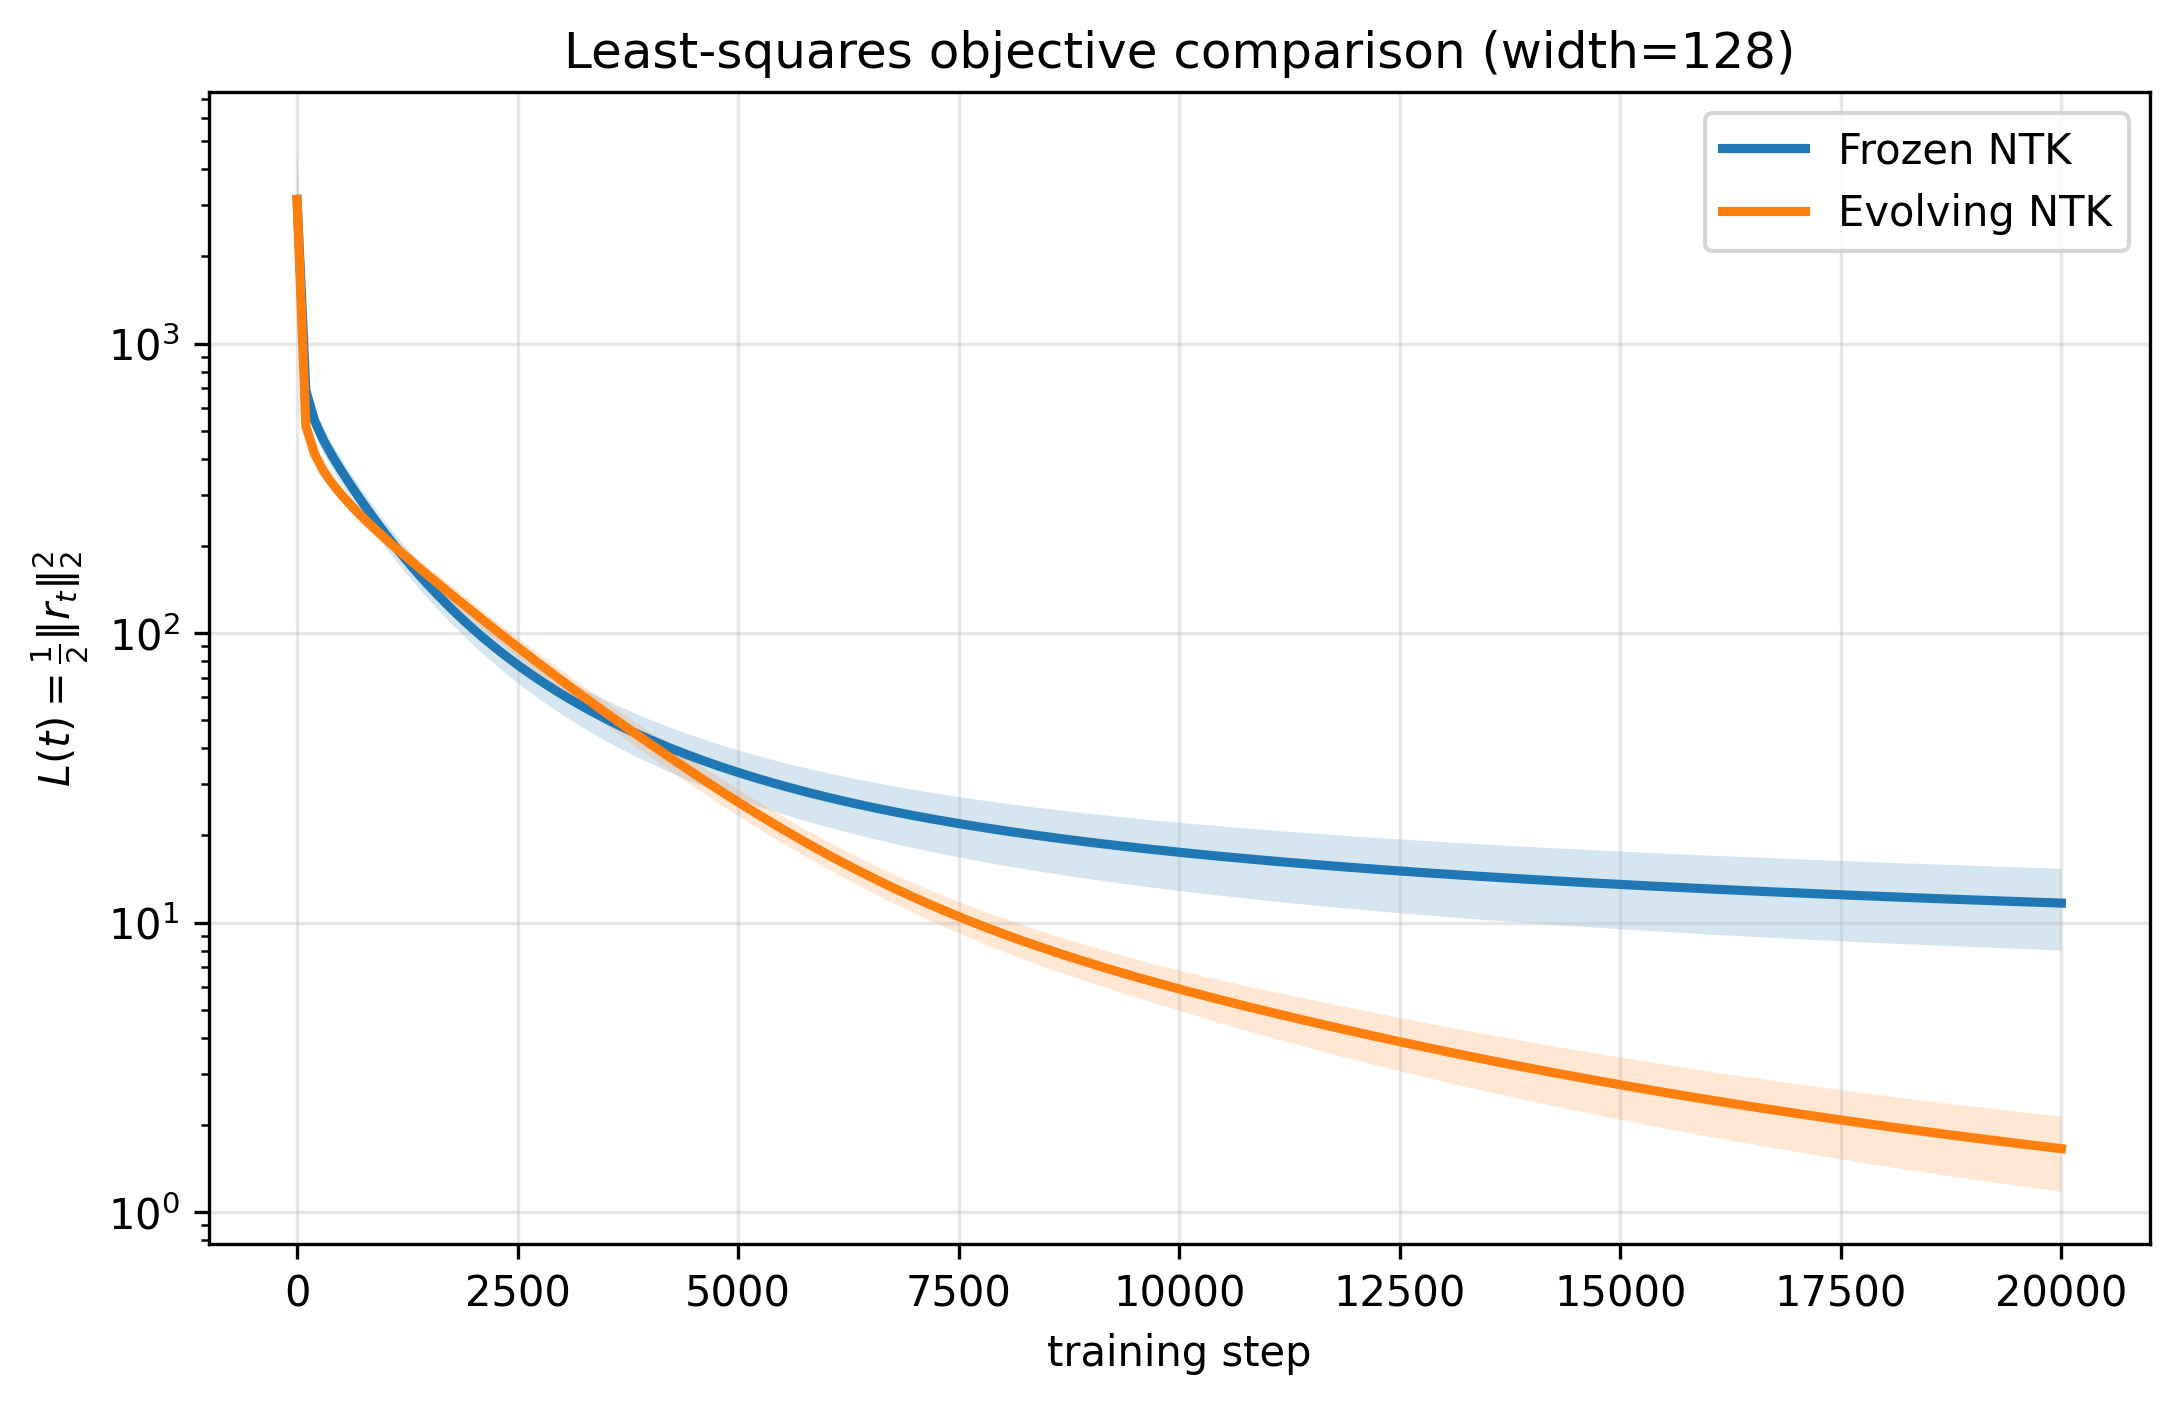
\includegraphics[width=\linewidth]{images/finite_width_evolving_results/train_ls_frozen_vs_evolving_w128.png}
		\caption{Width \(128\).}
	\end{subfigure}
	\hfill
	\begin{subfigure}[t]{0.48\textwidth}
		\centering
		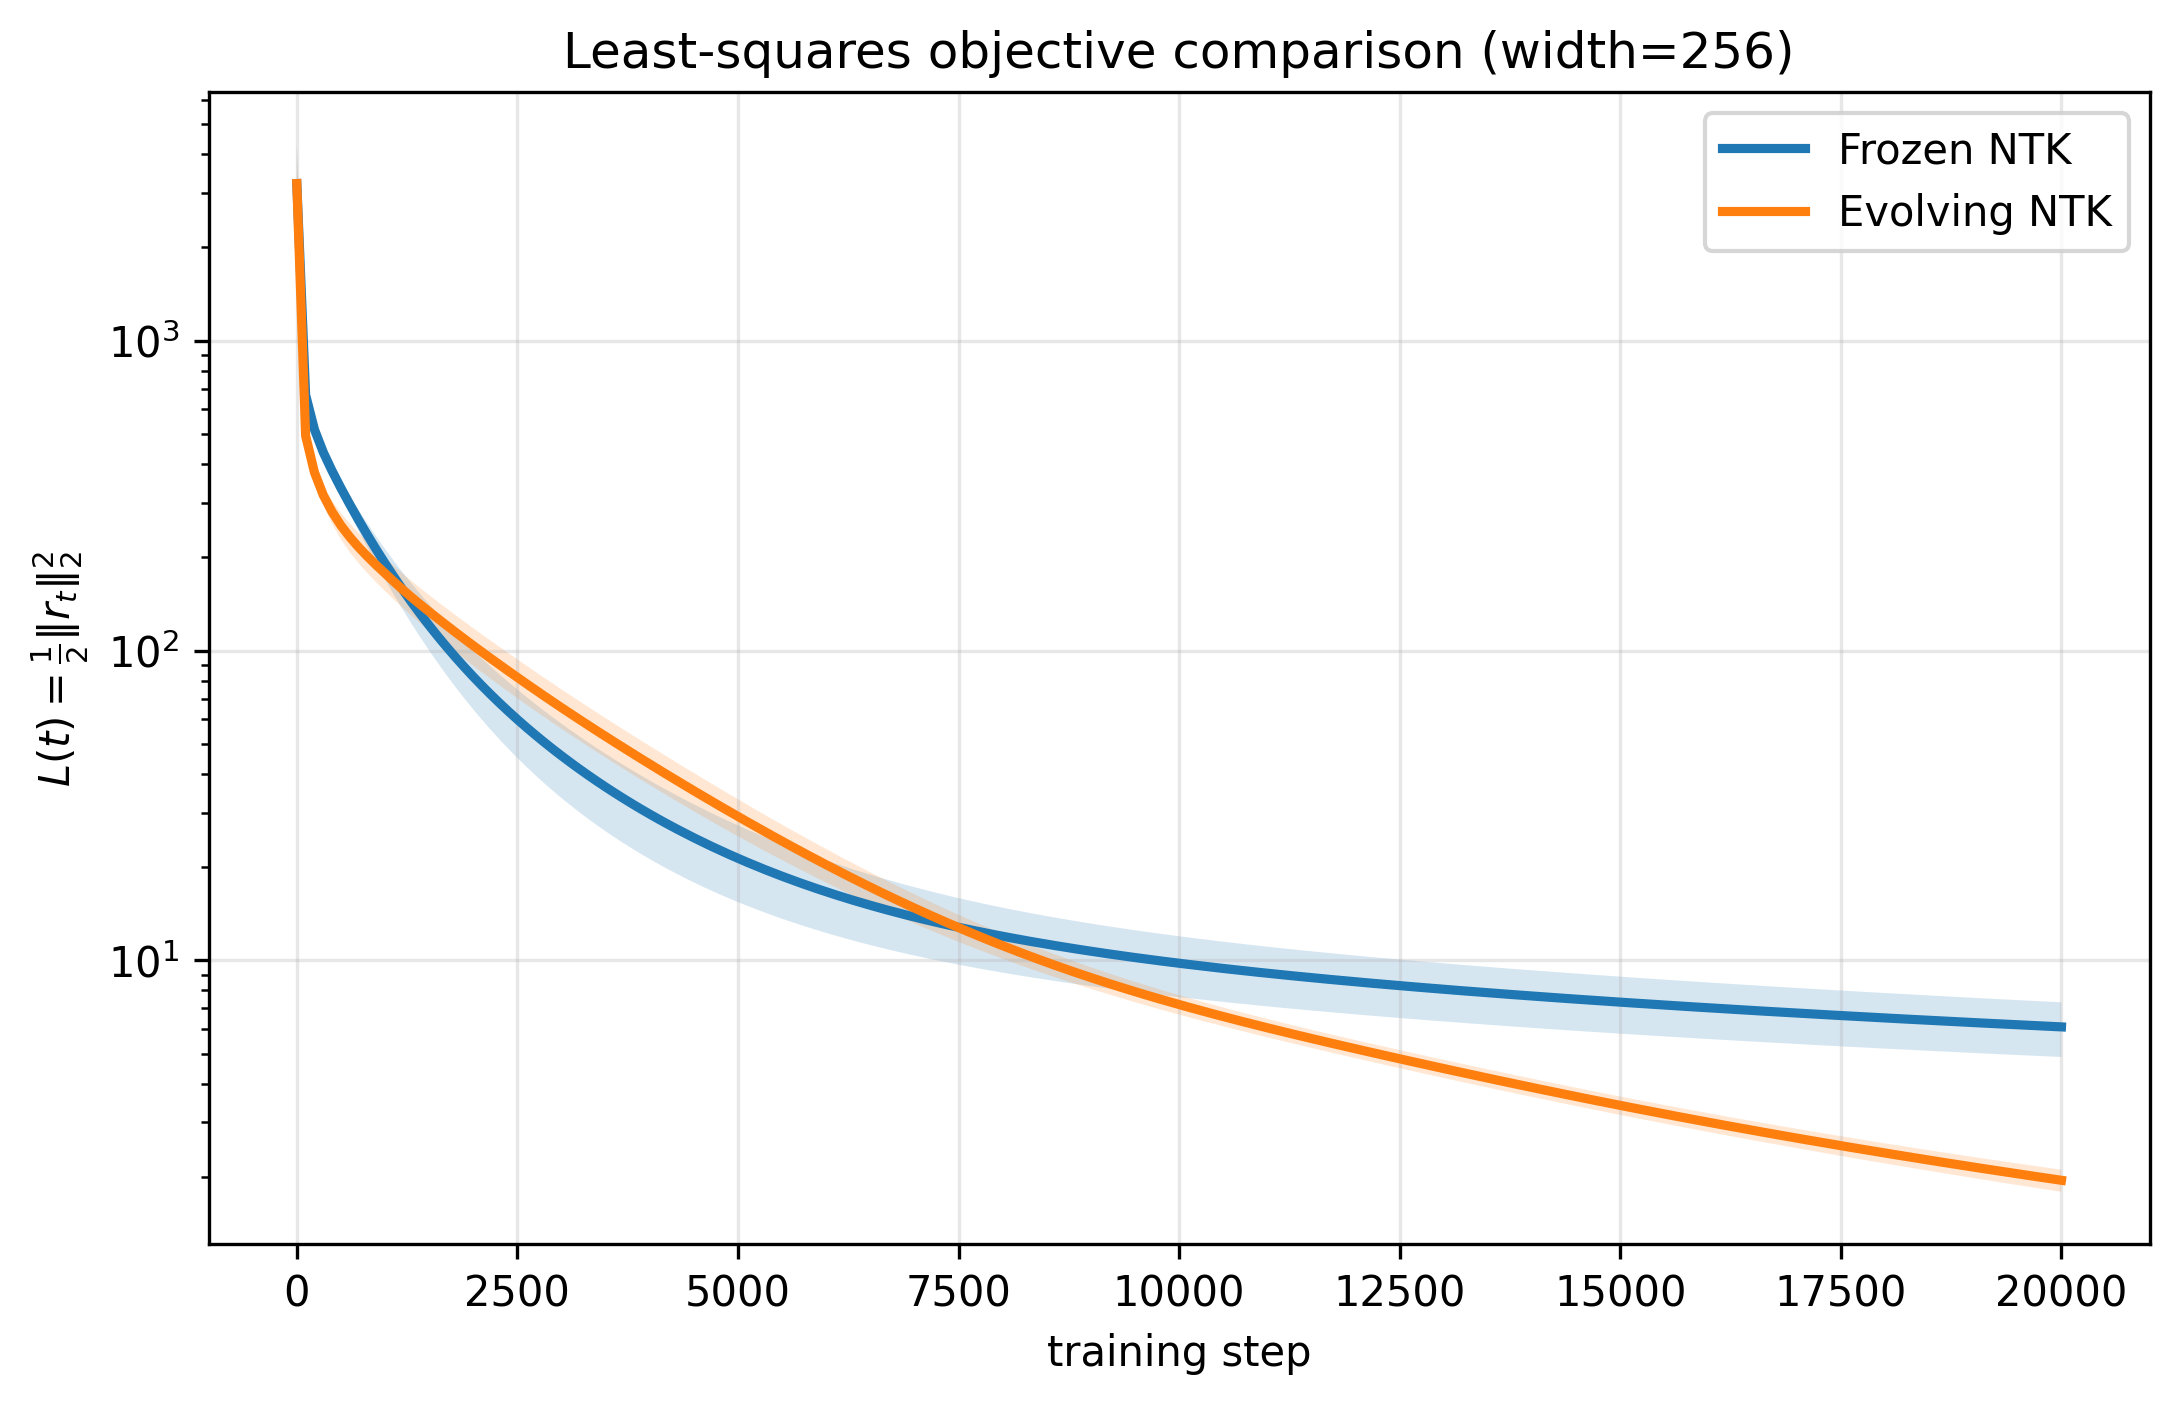
\includegraphics[width=\linewidth]{images/finite_width_evolving_results/train_ls_frozen_vs_evolving_w256.png}
		\caption{Width \(256\).}
	\end{subfigure}

	\vspace{0.6em}

	\begin{subfigure}[t]{0.48\textwidth}
		\centering
		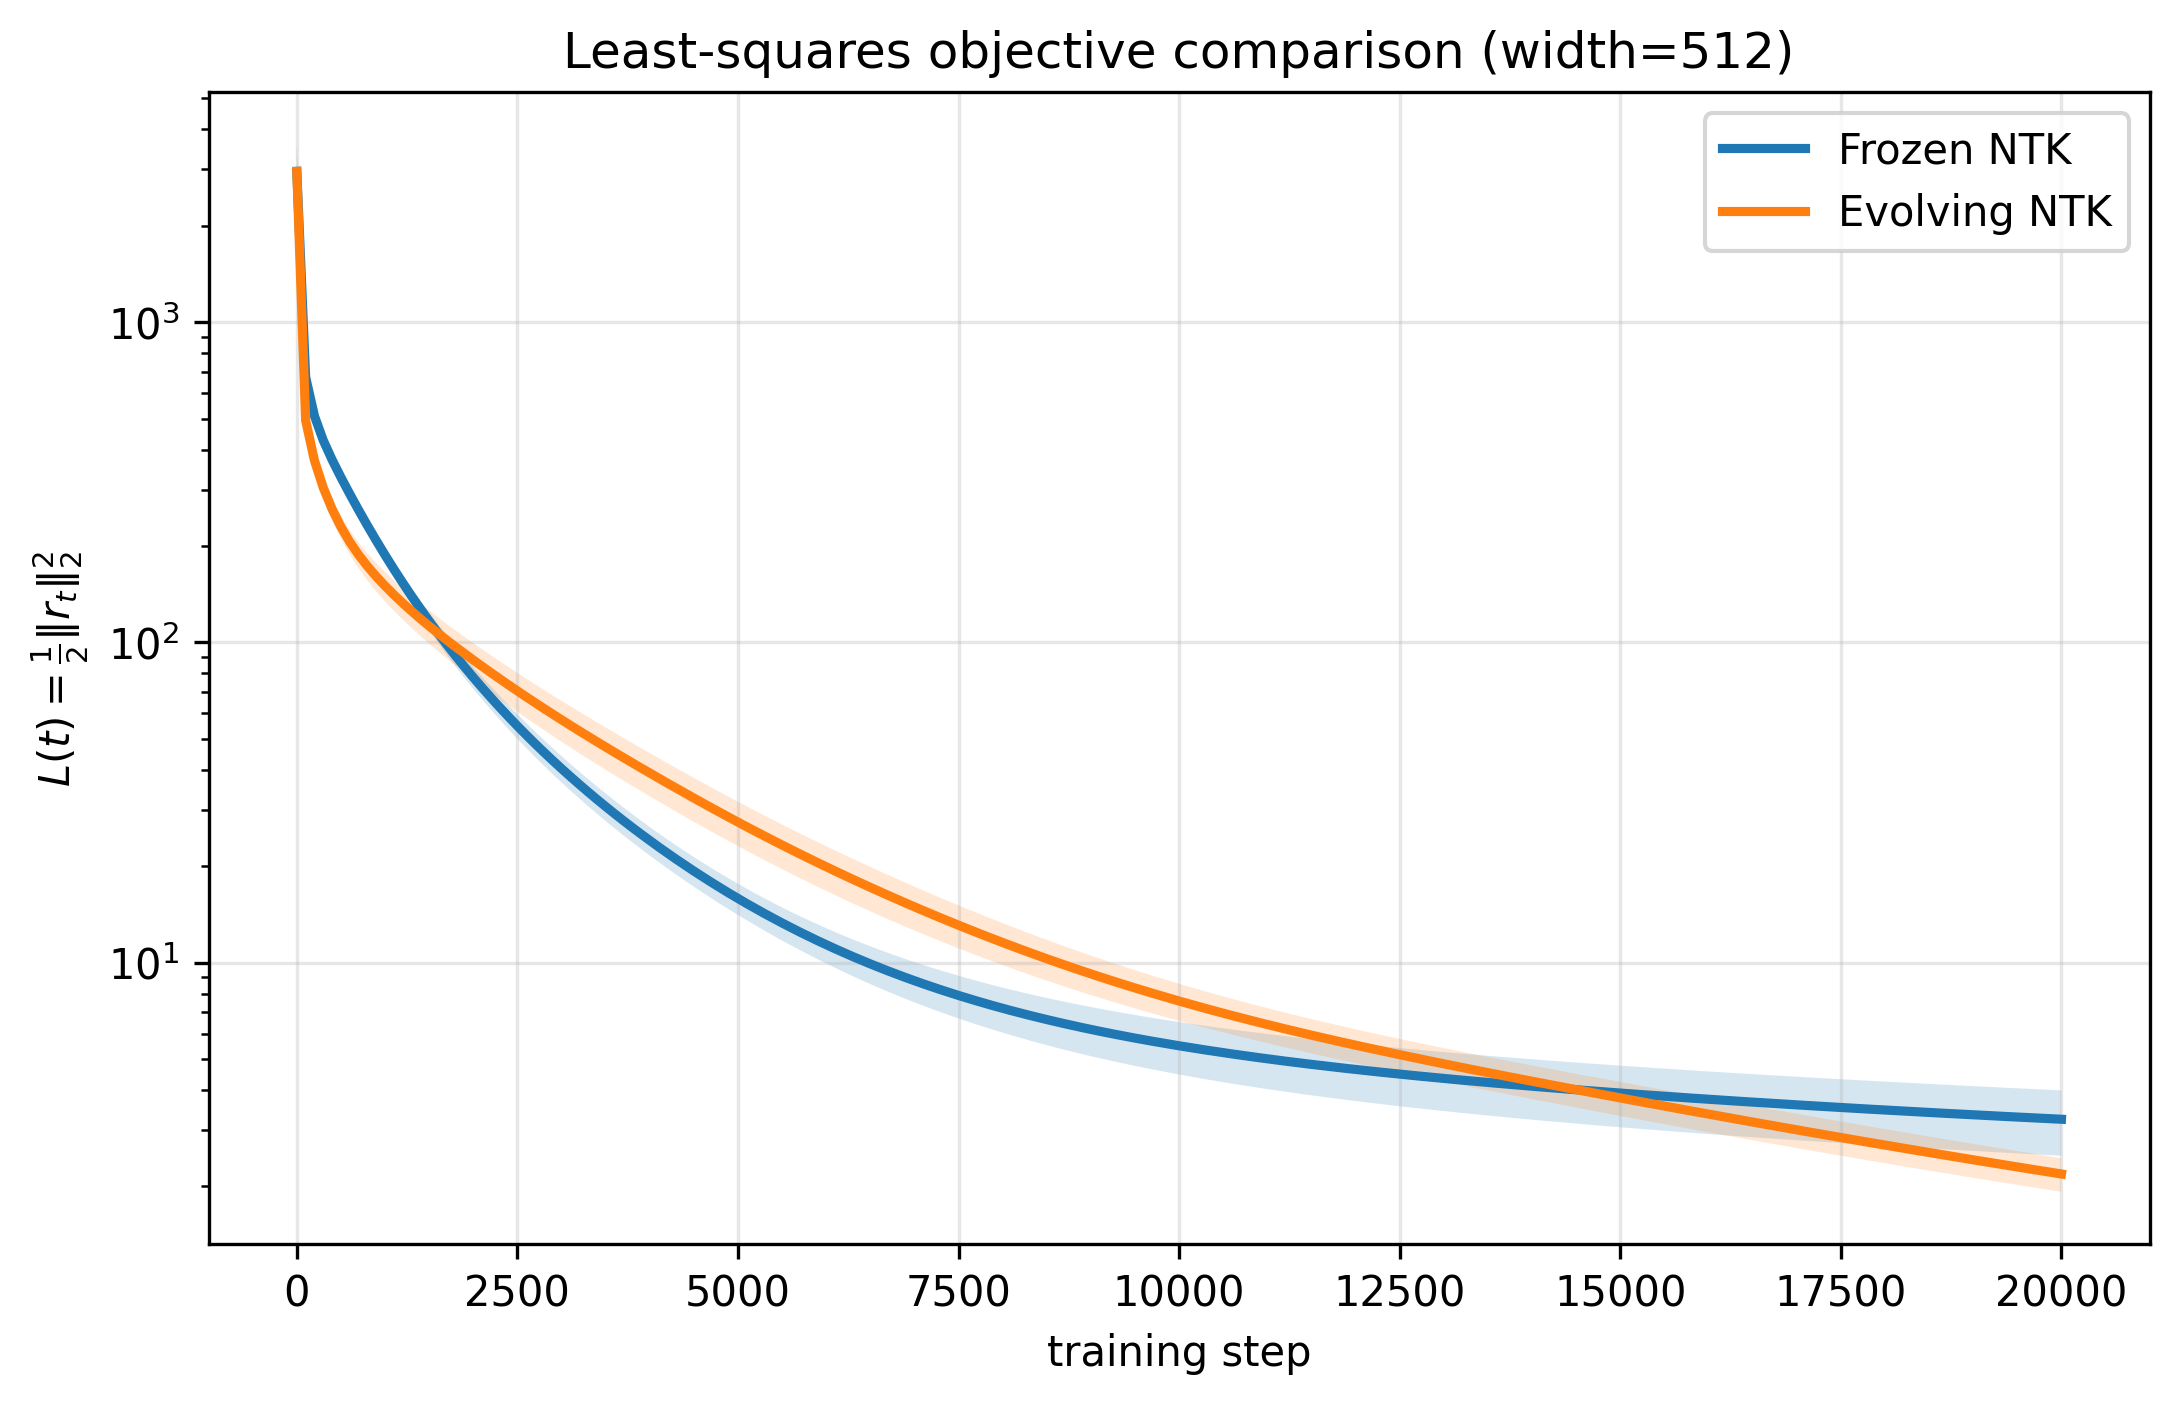
\includegraphics[width=\linewidth]{images/finite_width_evolving_results/train_ls_frozen_vs_evolving_w512.png}
		\caption{Width \(512\).}
	\end{subfigure}
	\hfill
	\begin{subfigure}[t]{0.48\textwidth}
		\centering
		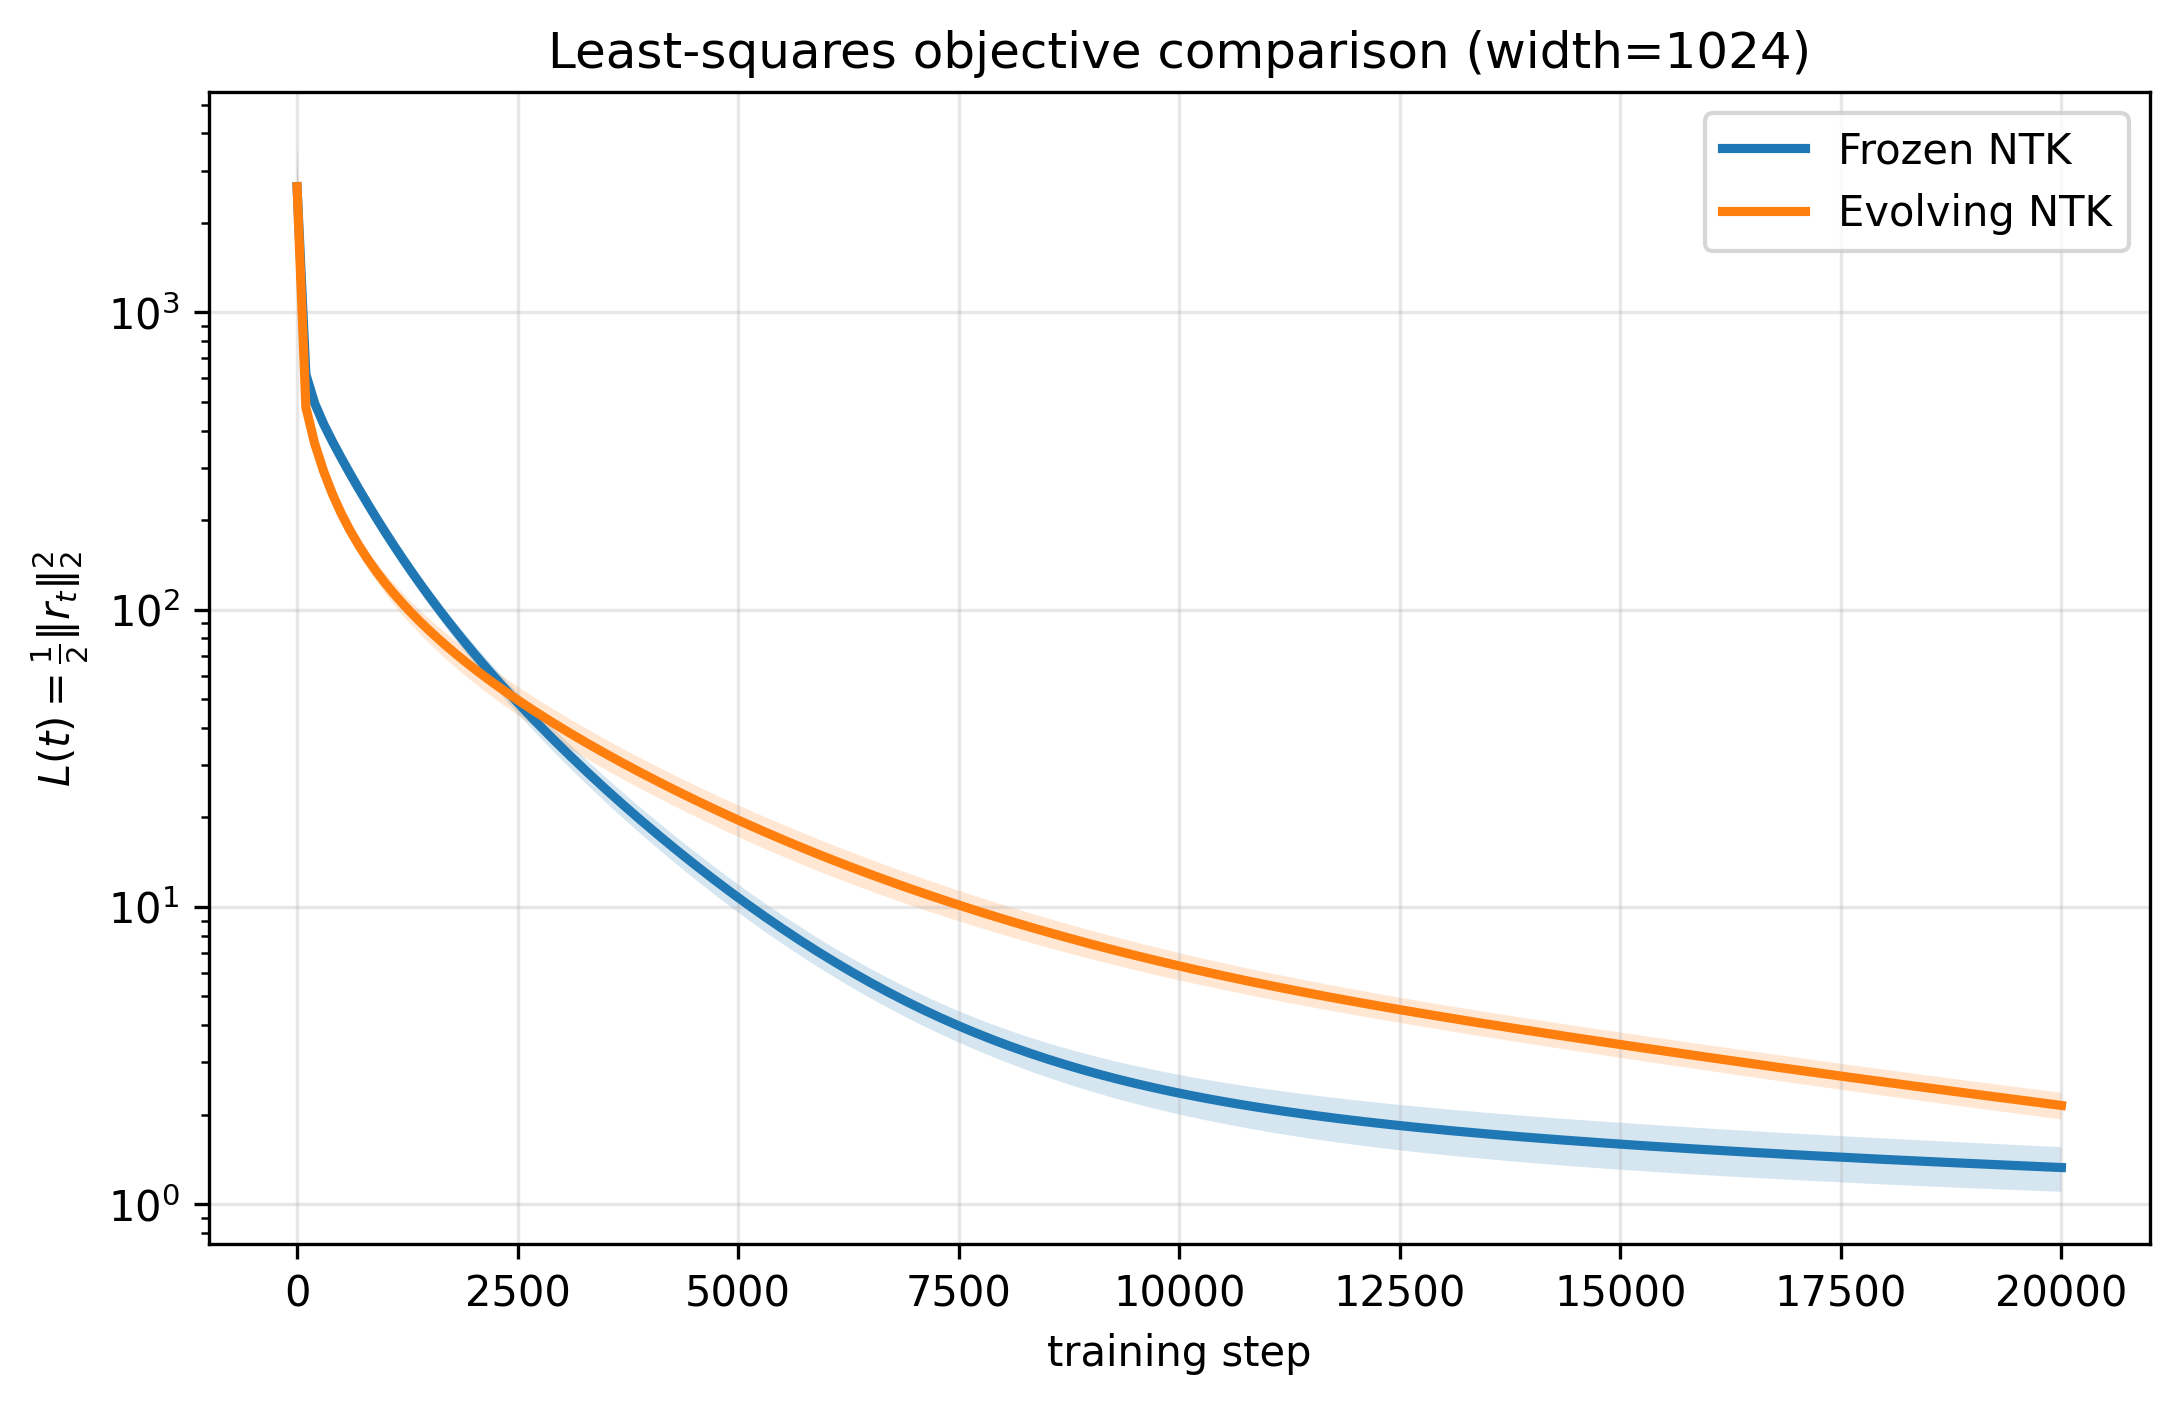
\includegraphics[width=\linewidth]{images/finite_width_evolving_results/train_ls_frozen_vs_evolving_w1024.png}
		\caption{Width \(1024\).}
	\end{subfigure}
	\caption{Least-squares objective comparison between frozen and evolving
		finite-width tangent-kernel dynamics across widths. The evolving kernel gives
		a clear improvement at widths \(128\) and \(256\), still improves the final
		objective at width \(512\), and loses its advantage by width \(1024\), where
		the frozen kernel reaches the lower final loss.}
	\label{fig:evolving-loss-by-width}
\end{figure}

In the frozen regime, the objective decreases more quickly as the width
increases. In the evolving regime, the curves are more tightly clustered across
widths. At widths \(128\) and \(256\), the evolving kernel reaches a lower final
objective than the frozen baseline. At width \(512\), the difference is smaller.
At width \(1024\), the frozen kernel reaches the lower final objective.

This raises the main question for the rest of the section: what changes in the
evolving tangent kernel allow it to help at small width, but not at large
width?

\subsection{Mode-wise decay, Fourier geometry, and spectral strength}
\label{subsec:results-evolving-joint}

To understand the loss comparison above, we examine three quantities together.
The mode-wise residual decay plots show how individual Fourier components are
learned over time. The subspace cosine similarity plots measure how closely the
eigenspaces of the evolving tangent-kernel remain aligned with the Fourier subspaces.
The spectral-strength plots measure the average eigenvalue inside each Fourier
block. This quantity can be read as the average strength with which the current
kernel acts on that Fourier subspace: larger spectral strength means that
residual components in that block are pushed down more strongly by the kernel
dynamics.

If the evolving kernel helps because it preserves Fourier geometry better, then
one would expect improved alignment in the subspaces over time. If instead it
helps by redistributing operator strength, then one should expect improved
decay of the low-frequency residual modes together with increased low-frequency
spectral strength, even if the Fourier alignment worsens.

\begin{figure}[!htbp]
	\centering

	\begin{subfigure}[t]{\textwidth}
		\centering
		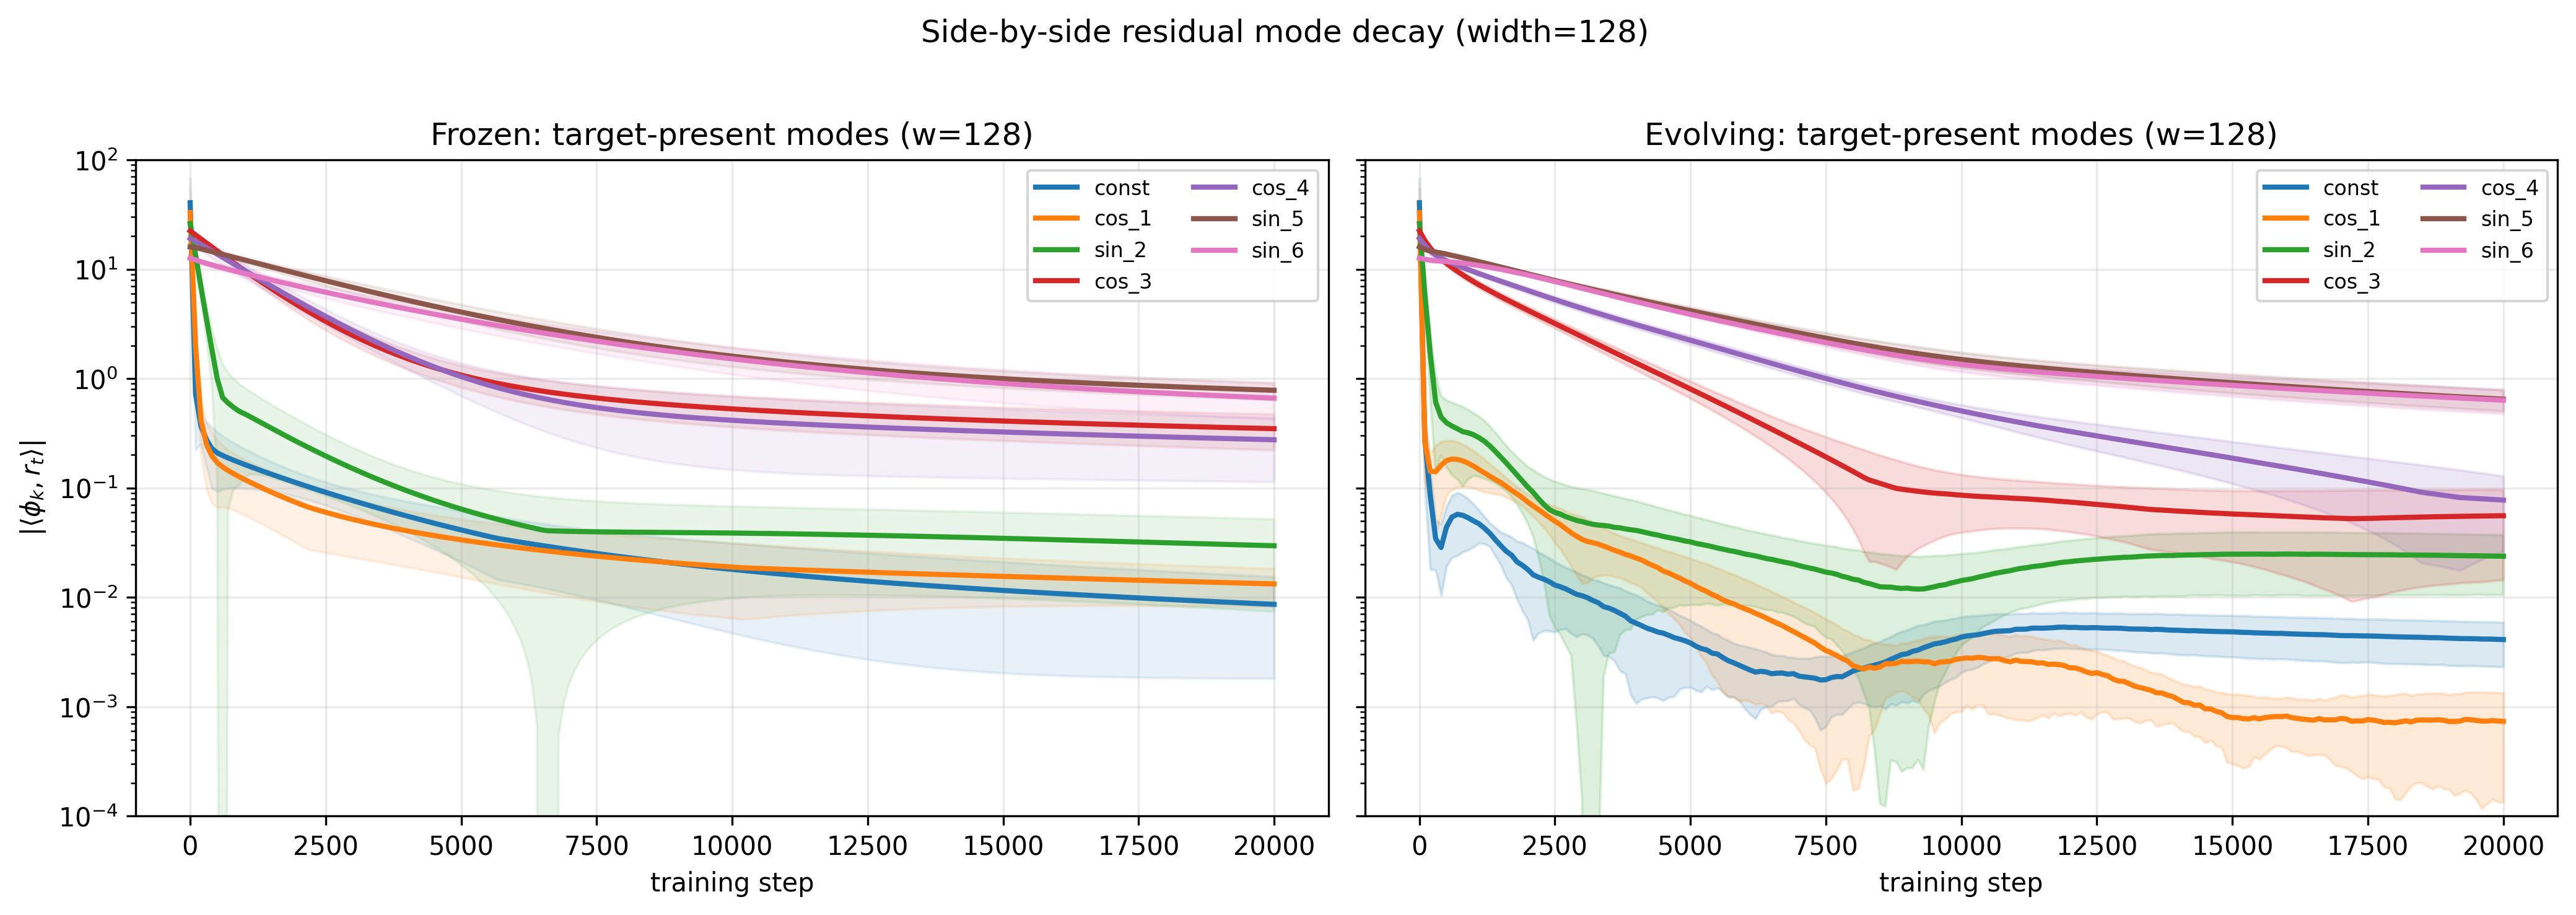
\includegraphics[width=\linewidth]{images/finite_width_evolving_results/side_by_side_residual_decay_w128.png}
		\caption{Mode-wise residual decay.}
	\end{subfigure}

	\vspace{0.8em}

	\begin{subfigure}[t]{\textwidth}
		\centering
		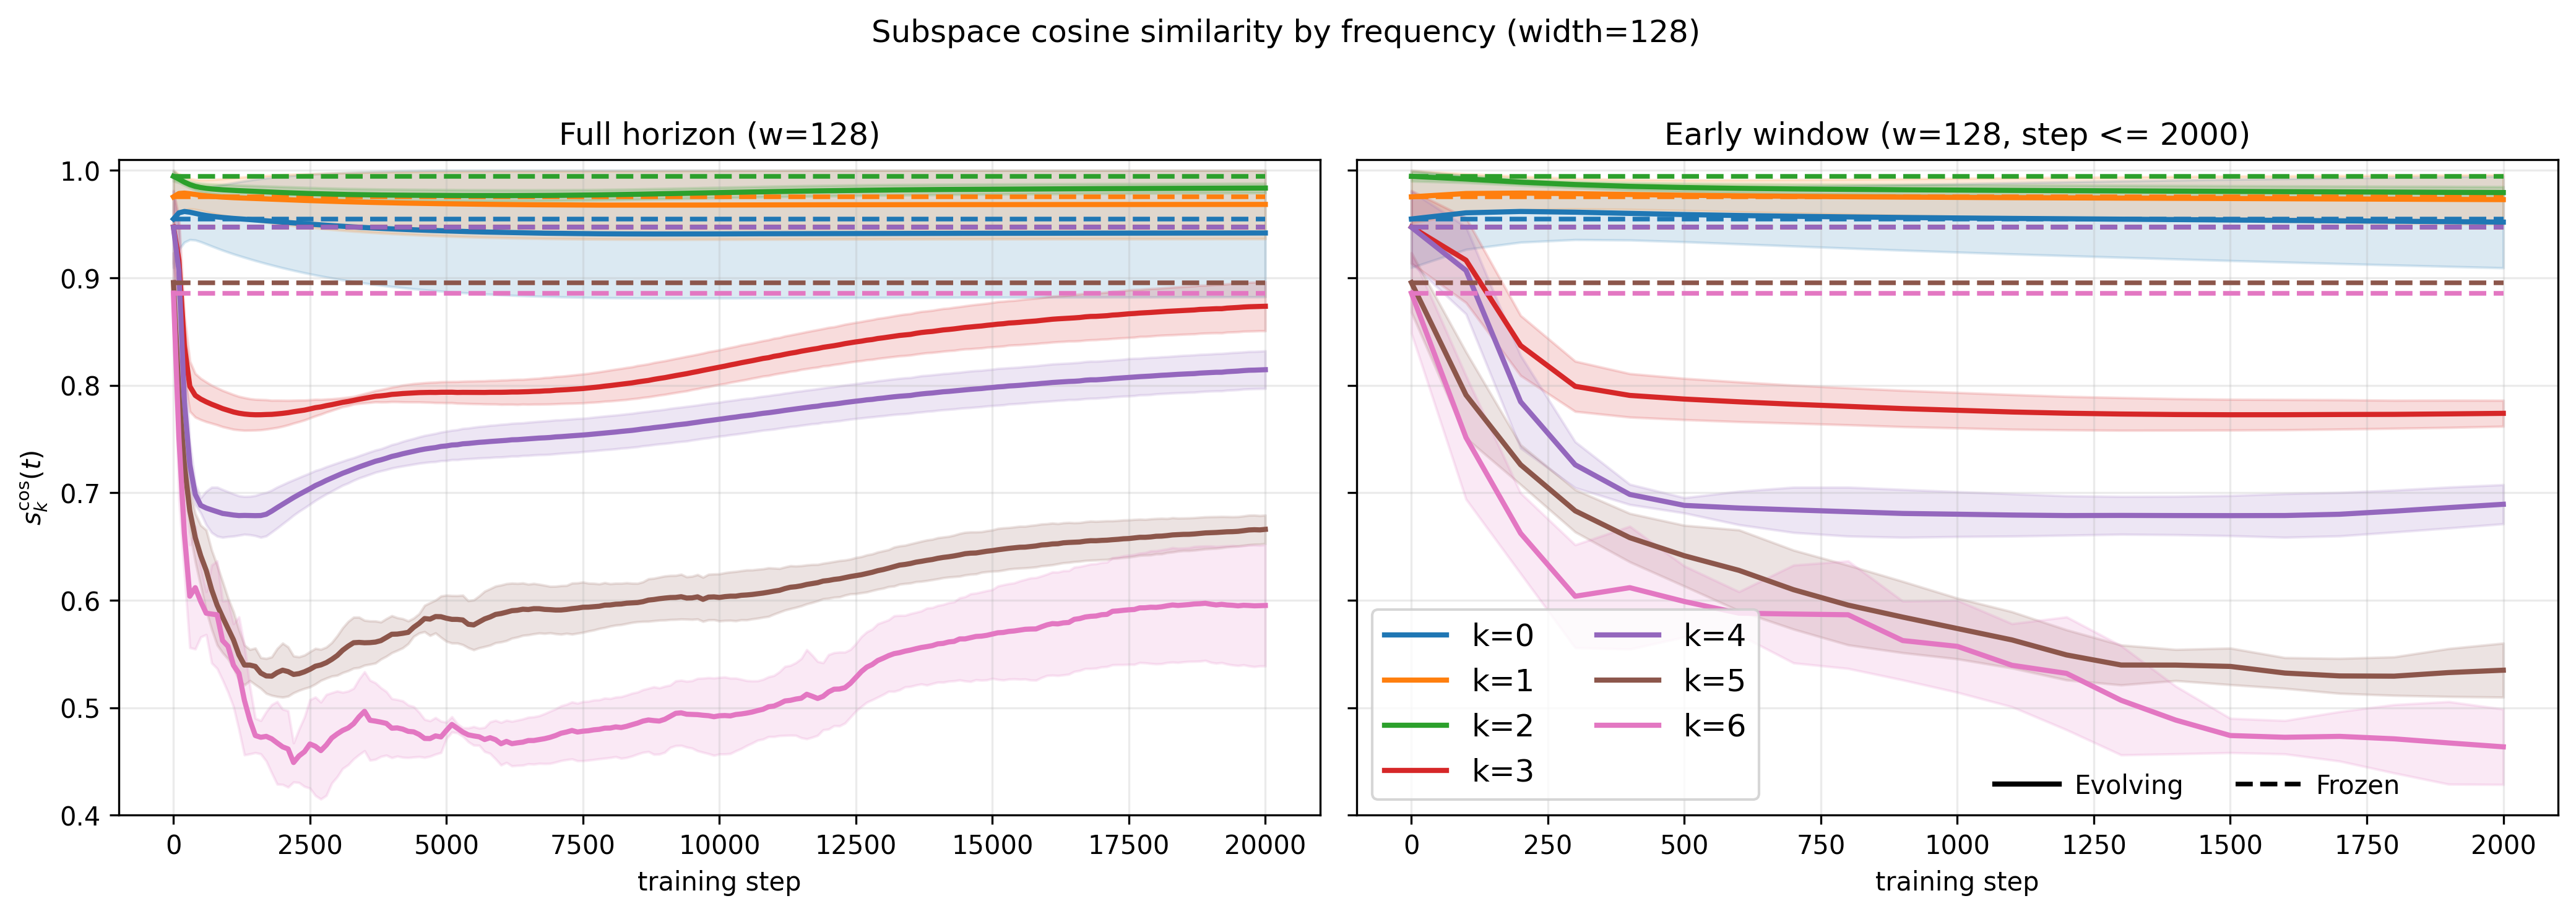
\includegraphics[width=\linewidth]{images/finite_width_evolving_results/rms_cos_alignment_by_freq_w128.png}
		\caption{Subspace cosine similarity.}
	\end{subfigure}

	\vspace{0.8em}

	\begin{subfigure}[t]{\textwidth}
		\centering
		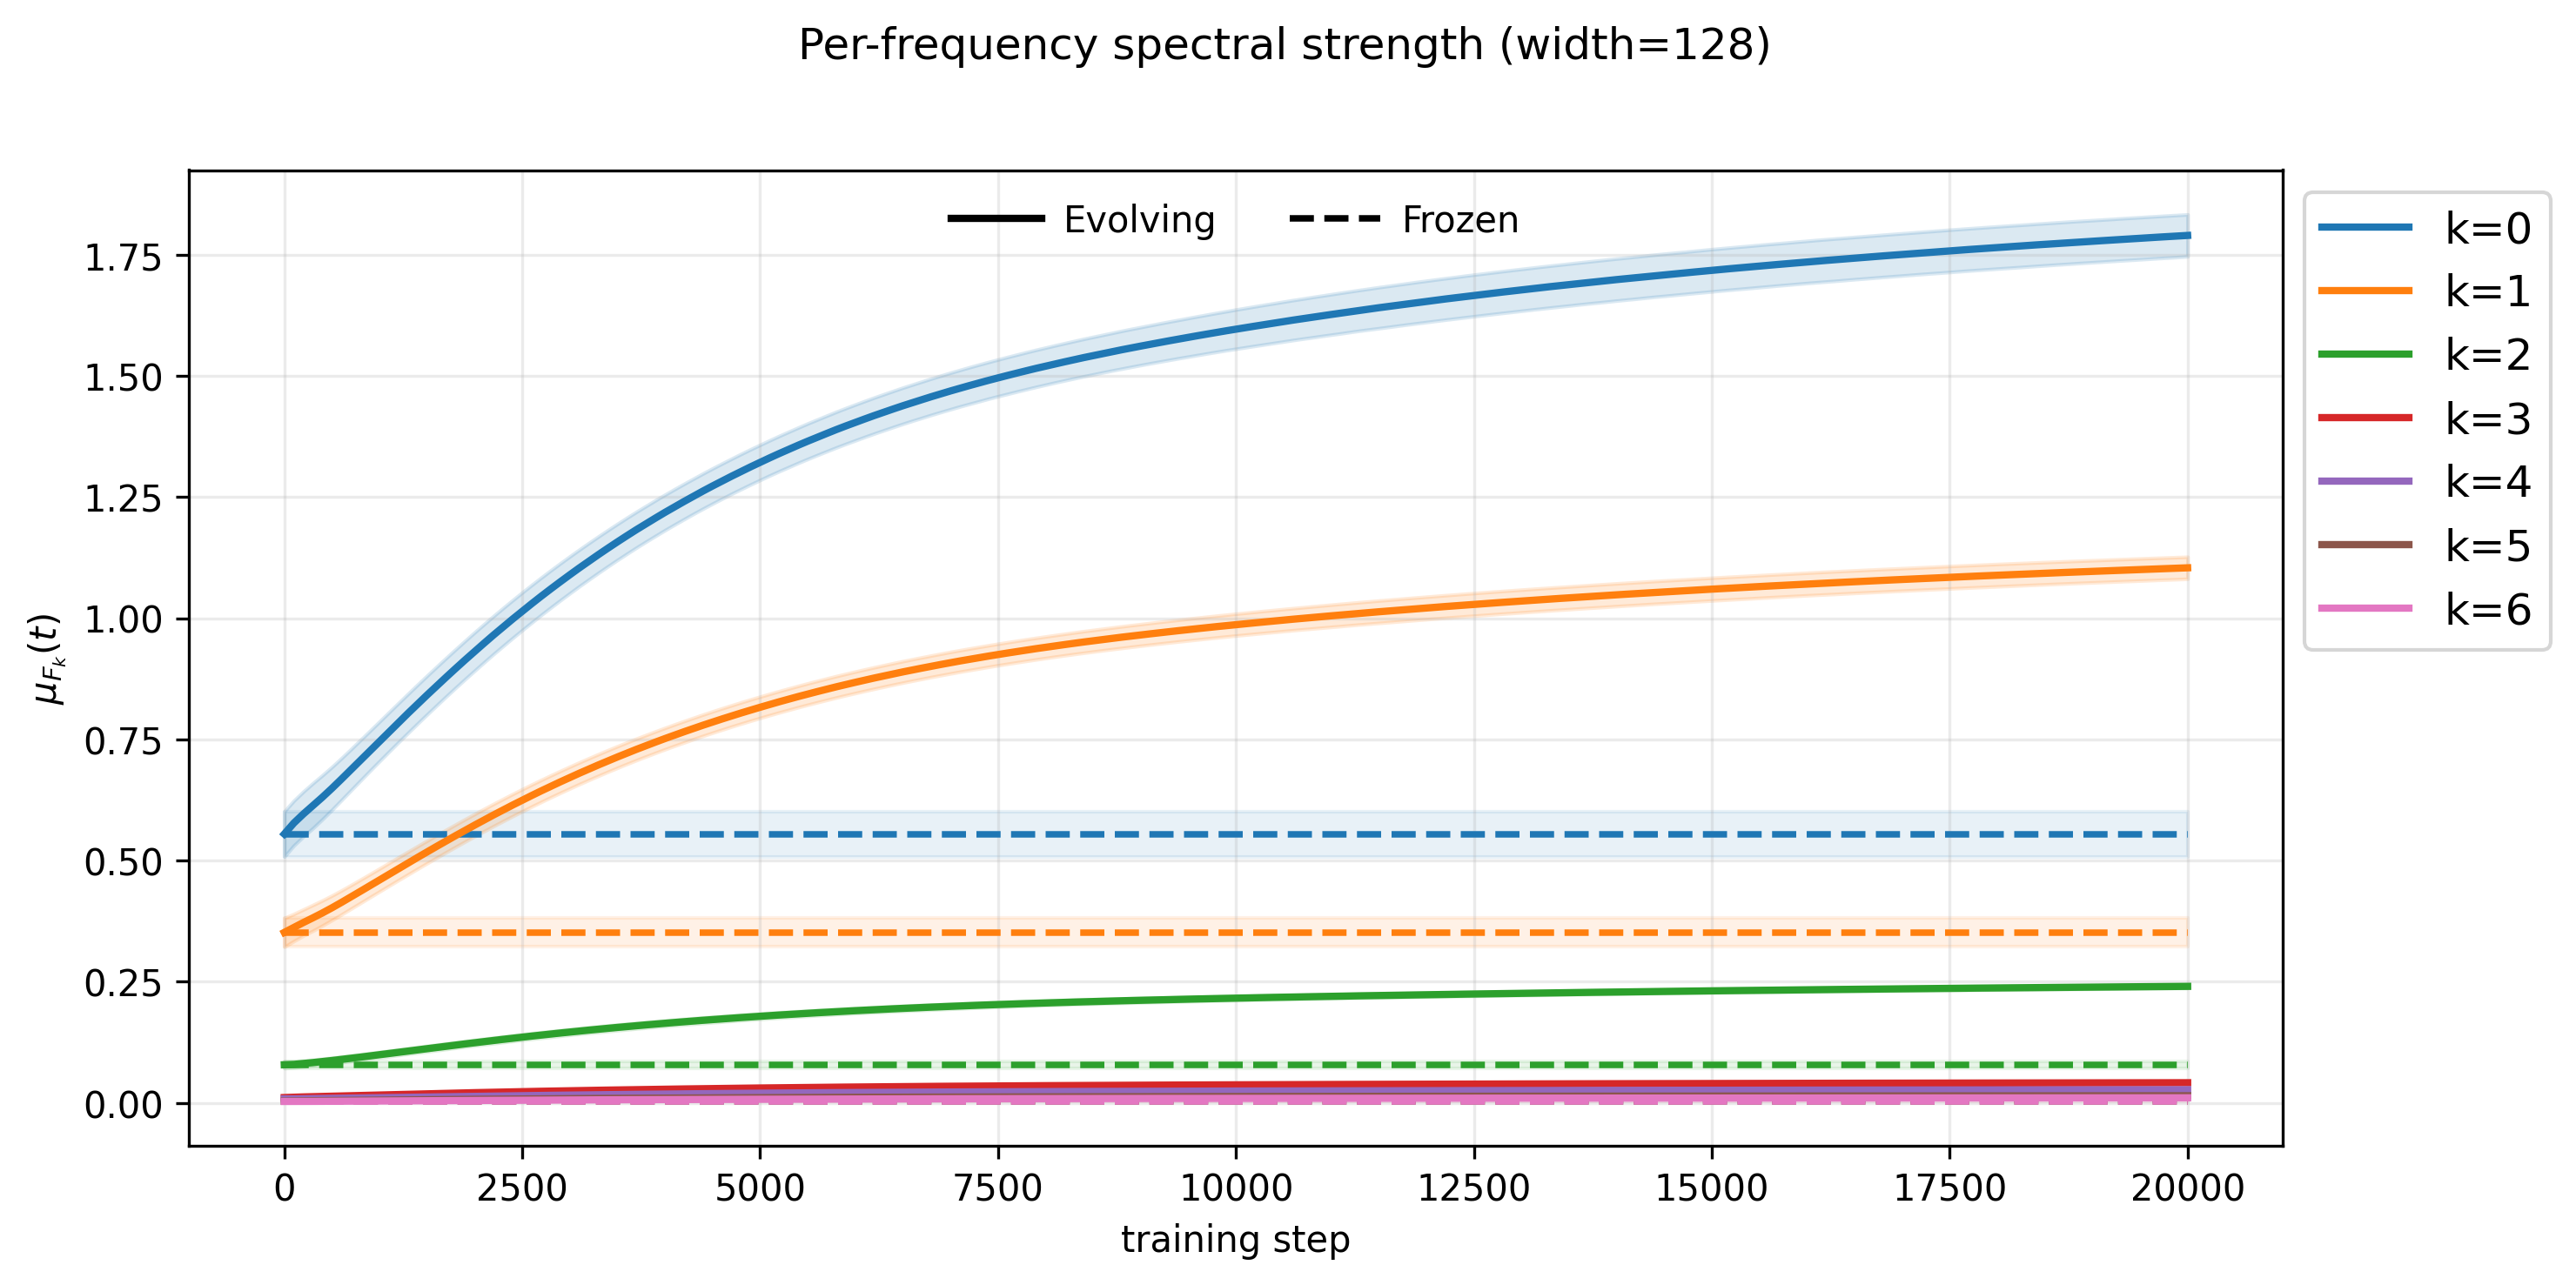
\includegraphics[width=\linewidth]{images/finite_width_evolving_results/spectral_strength_by_freq_w128.png}
		\caption{Per-frequency spectral strength.}
	\end{subfigure}

	\caption{Joint diagnostics for the evolving finite-width tangent kernel at
		width \(128\). The top panel compares frozen and evolving residual decay for
		the target-present modes. The middle panel measures Fourier-subspace
		alignment. The bottom panel measures the average tangent-kernel strength
		inside each Fourier block.}
	\label{fig:evolving-joint-w128}
\end{figure}

\begin{figure}[!htbp]
	\centering

	\begin{subfigure}[t]{\textwidth}
		\centering
		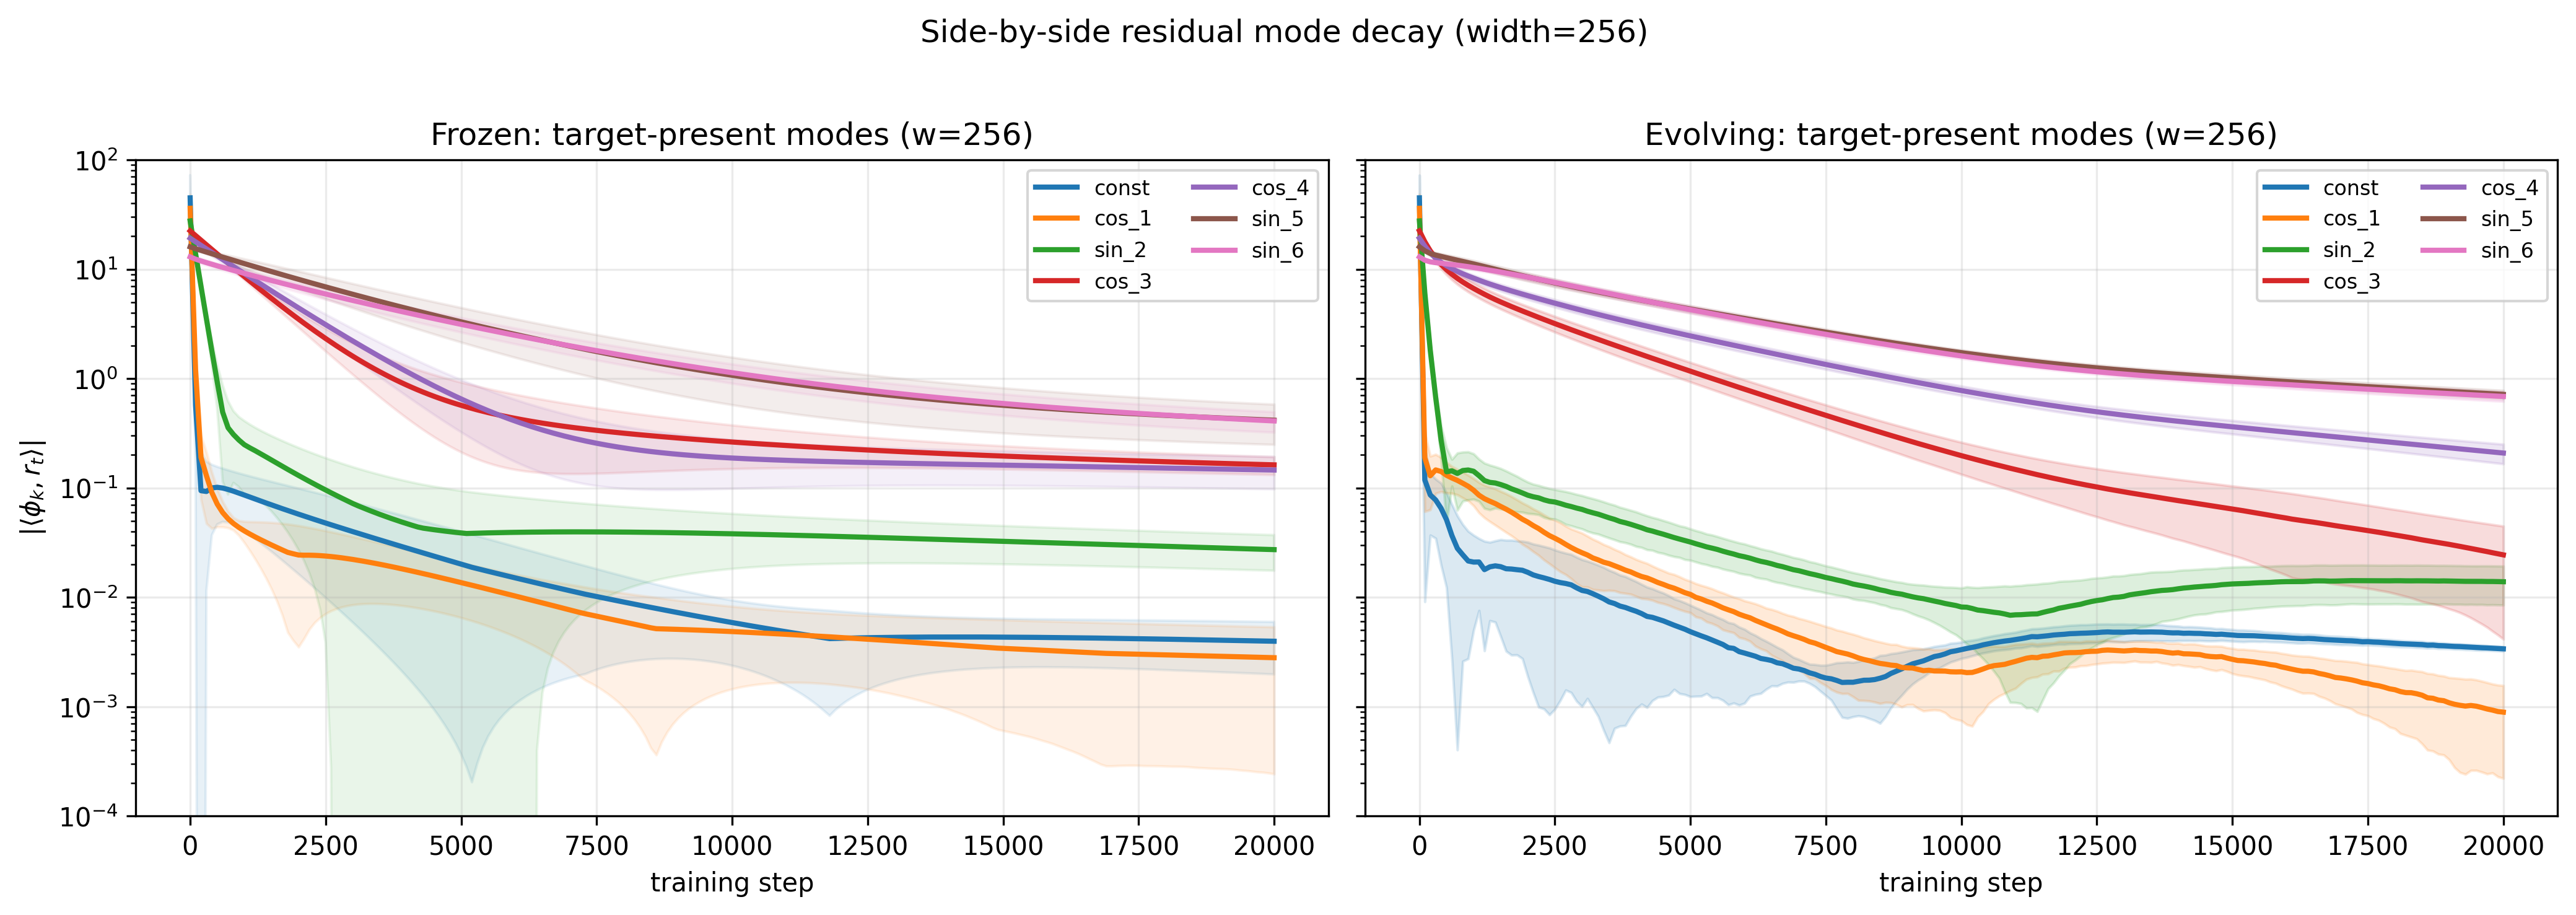
\includegraphics[width=\linewidth]{images/finite_width_evolving_results/side_by_side_residual_decay_w256.png}
		\caption{Mode-wise residual decay.}
	\end{subfigure}

	\vspace{0.8em}

	\begin{subfigure}[t]{\textwidth}
		\centering
		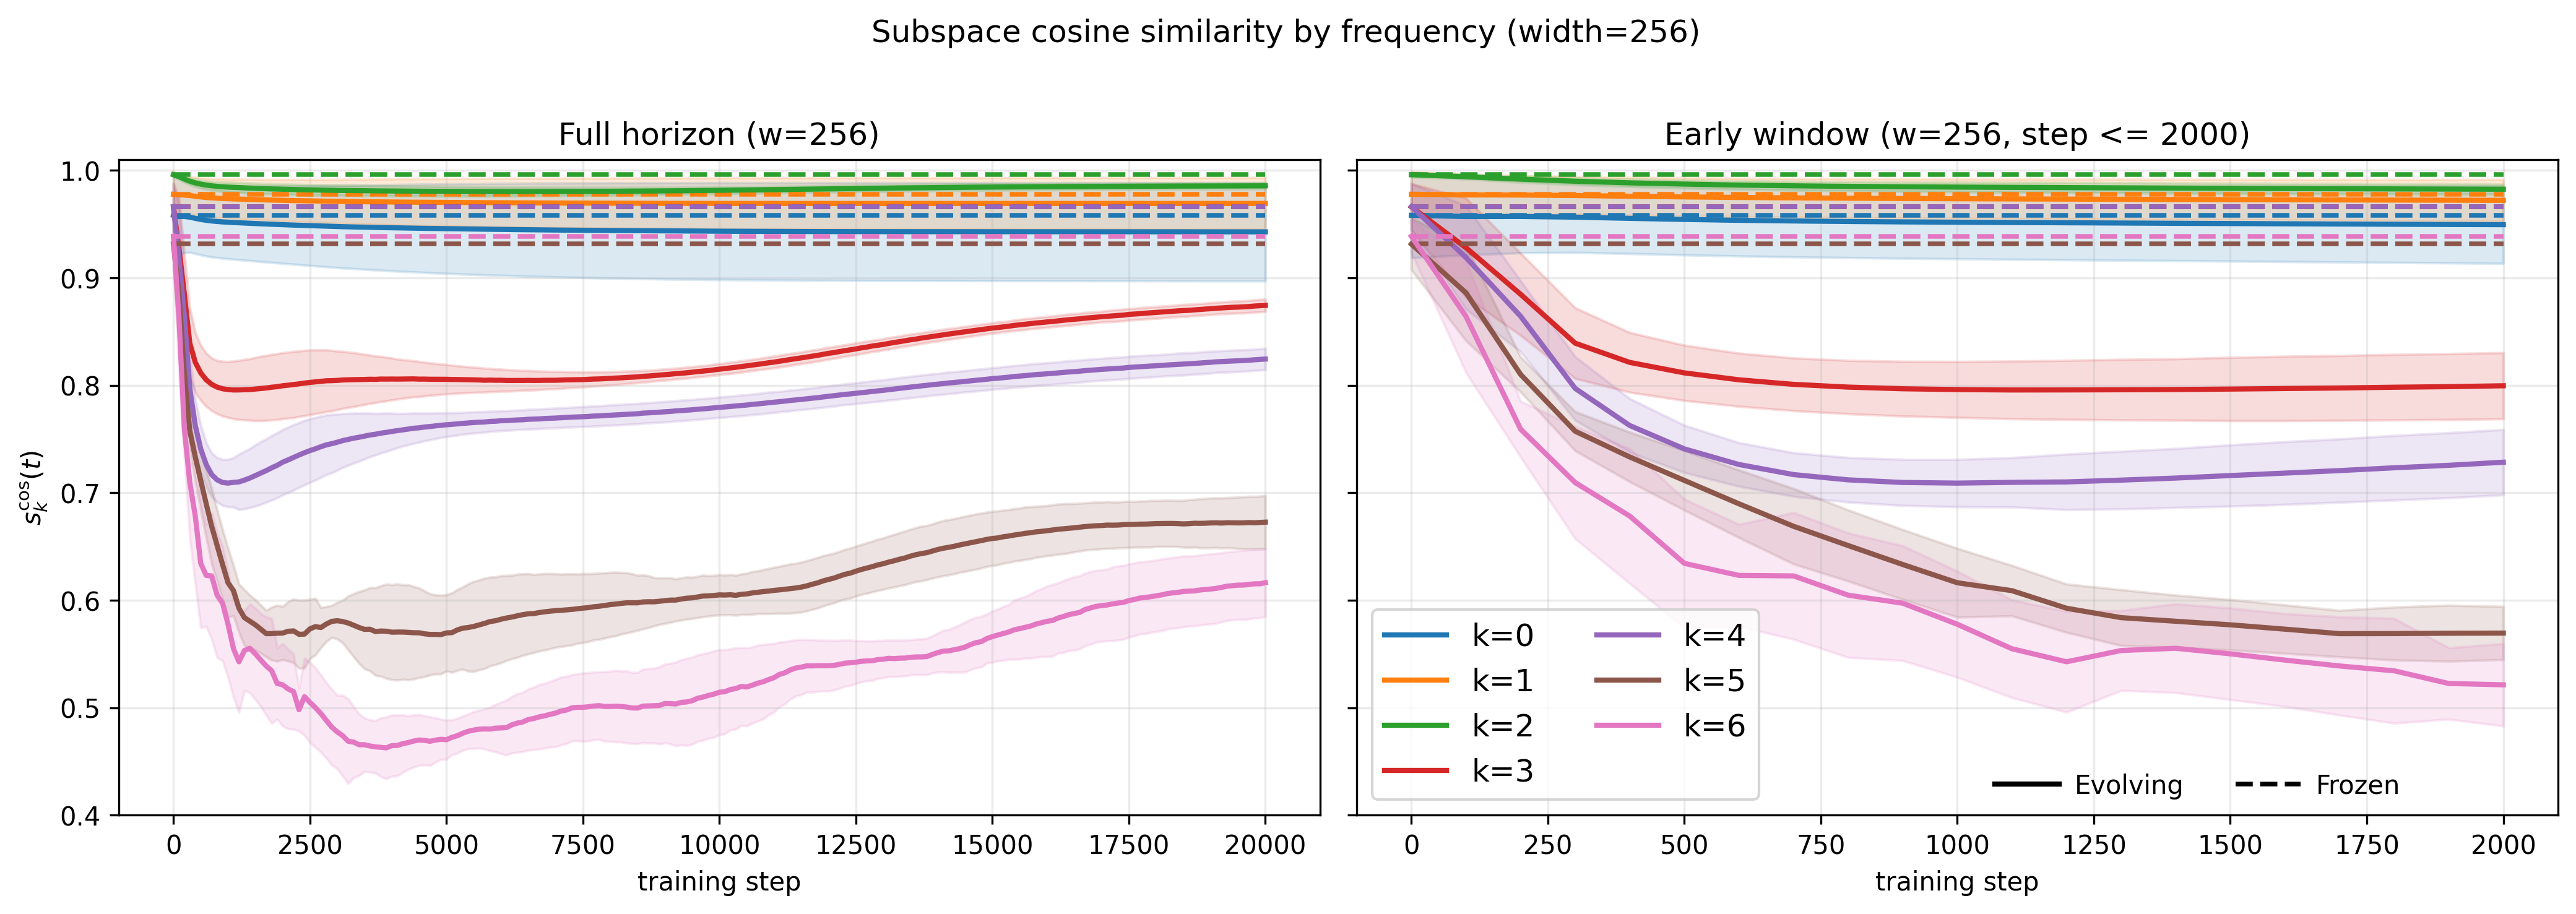
\includegraphics[width=\linewidth]{images/finite_width_evolving_results/rms_cos_alignment_by_freq_w256.png}
		\caption{Subspace cosine similarity.}
	\end{subfigure}

	\vspace{0.8em}

	\begin{subfigure}[t]{\textwidth}
		\centering
		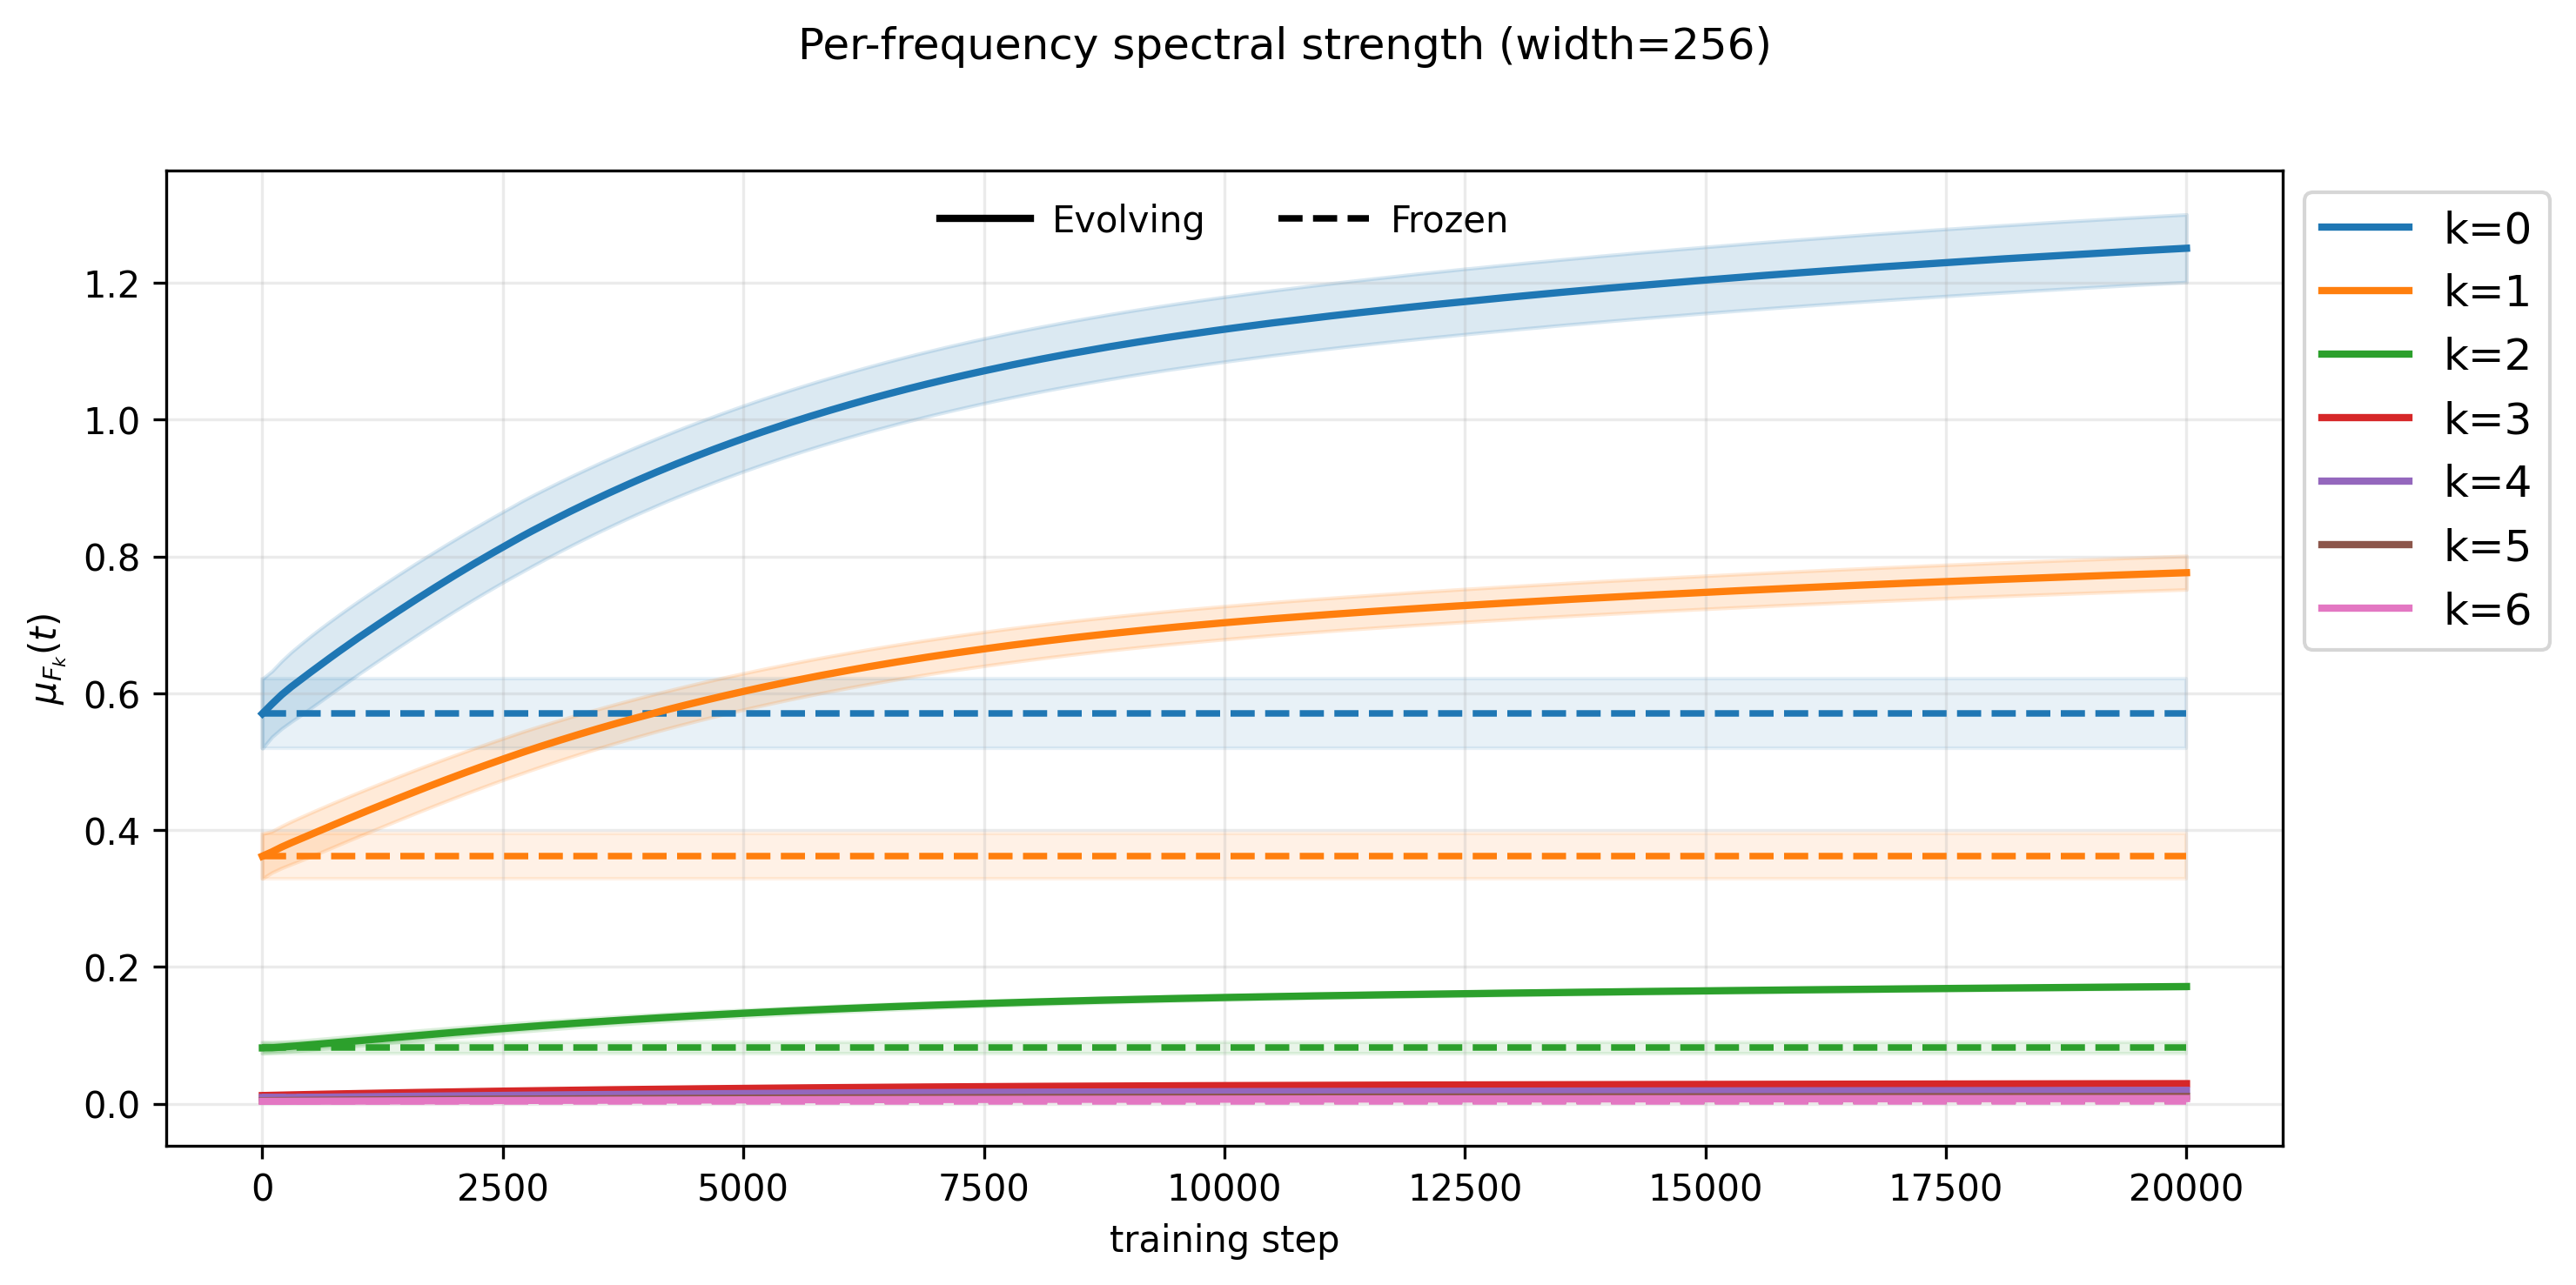
\includegraphics[width=\linewidth]{images/finite_width_evolving_results/spectral_strength_by_freq_w256.png}
		\caption{Per-frequency spectral strength.}
	\end{subfigure}

	\caption{Joint diagnostics for the evolving finite-width tangent kernel at
		width \(256\).}
	\label{fig:evolving-joint-w256}
\end{figure}

\begin{figure}[!htbp]
	\centering

	\begin{subfigure}[t]{\textwidth}
		\centering
		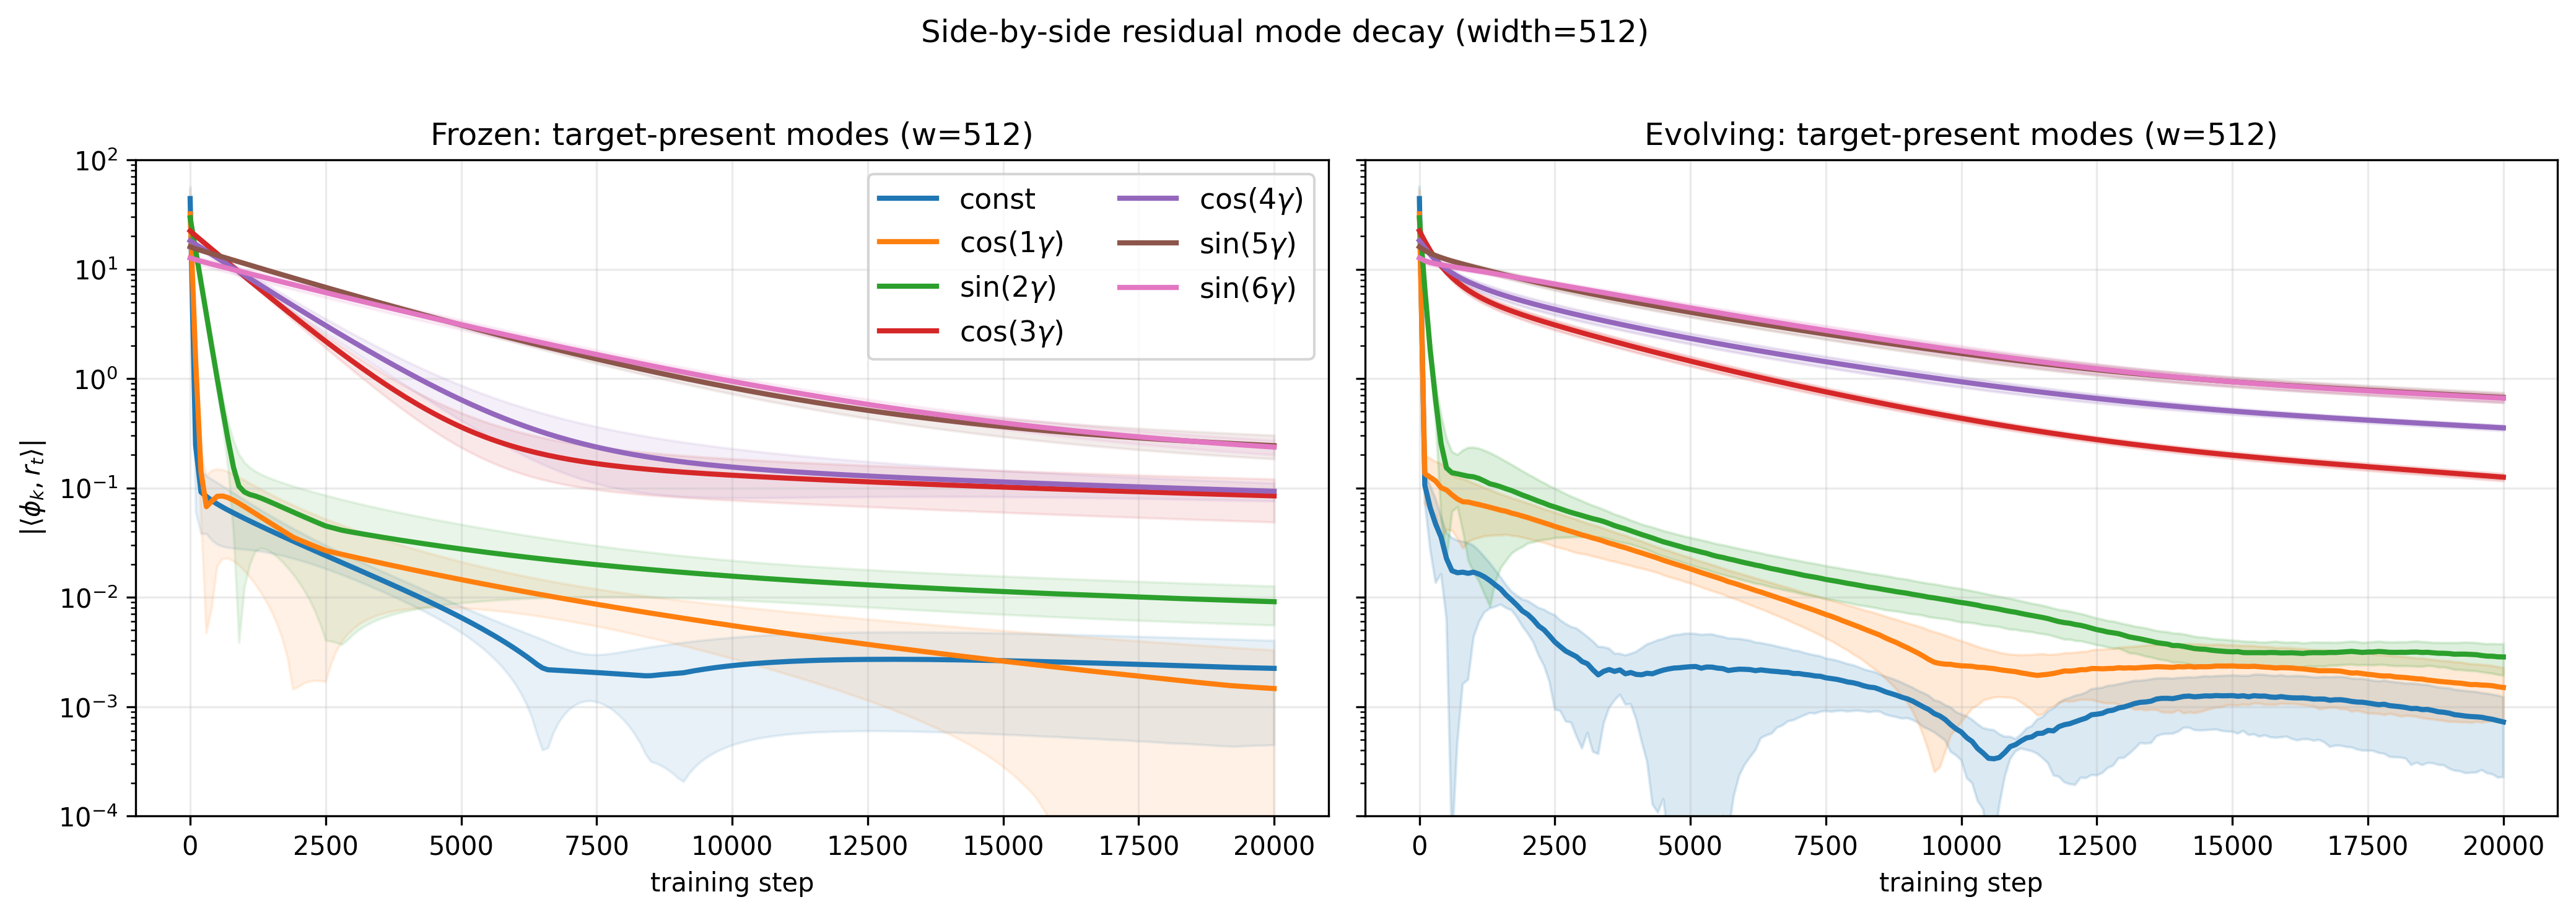
\includegraphics[width=\linewidth]{images/finite_width_evolving_results/side_by_side_residual_decay_w512.png}
		\caption{Mode-wise residual decay.}
	\end{subfigure}

	\vspace{0.8em}

	\begin{subfigure}[t]{\textwidth}
		\centering
		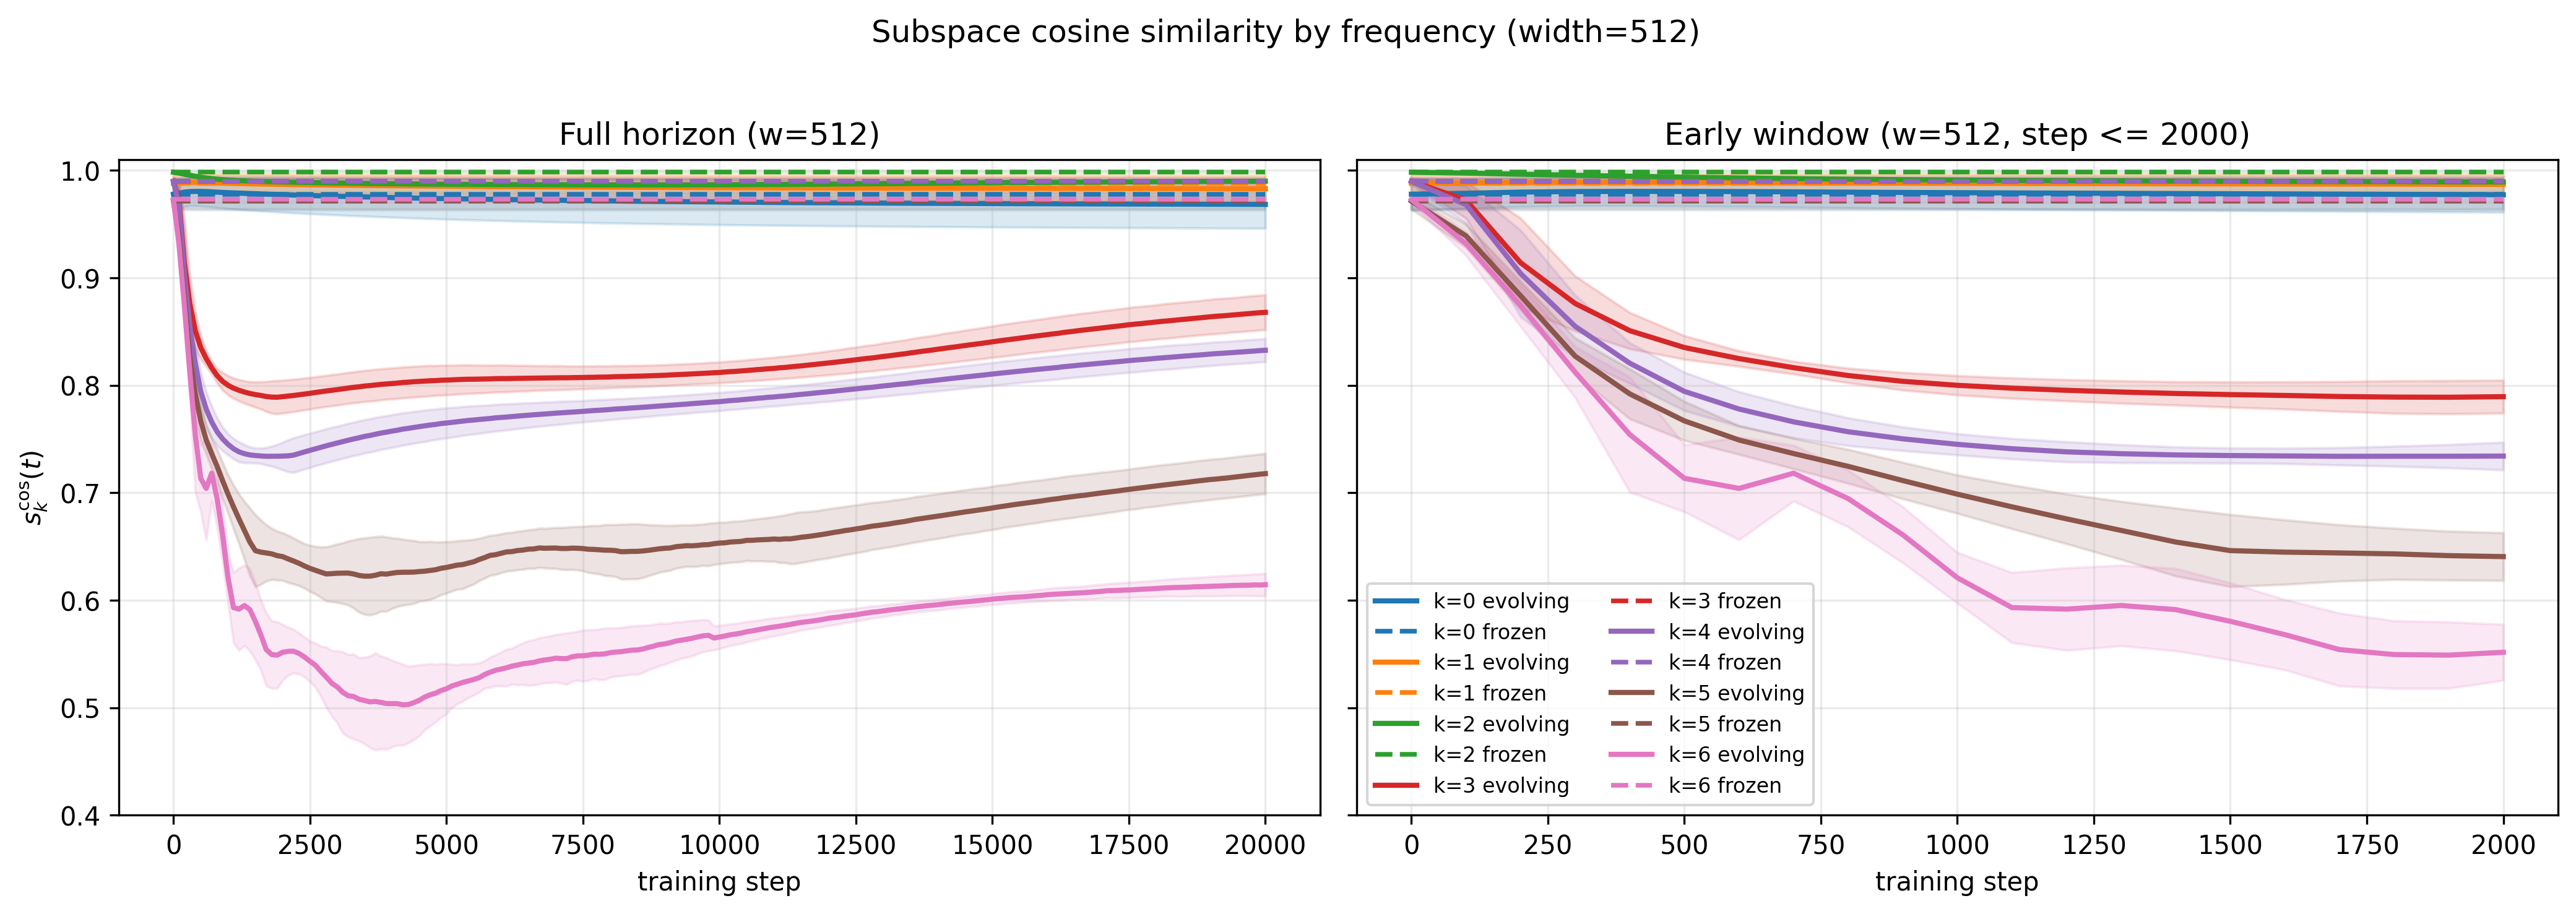
\includegraphics[width=\linewidth]{images/finite_width_evolving_results/rms_cos_alignment_by_freq_w512.png}
		\caption{Subspace cosine similarity.}
	\end{subfigure}

	\vspace{0.8em}

	\begin{subfigure}[t]{\textwidth}
		\centering
		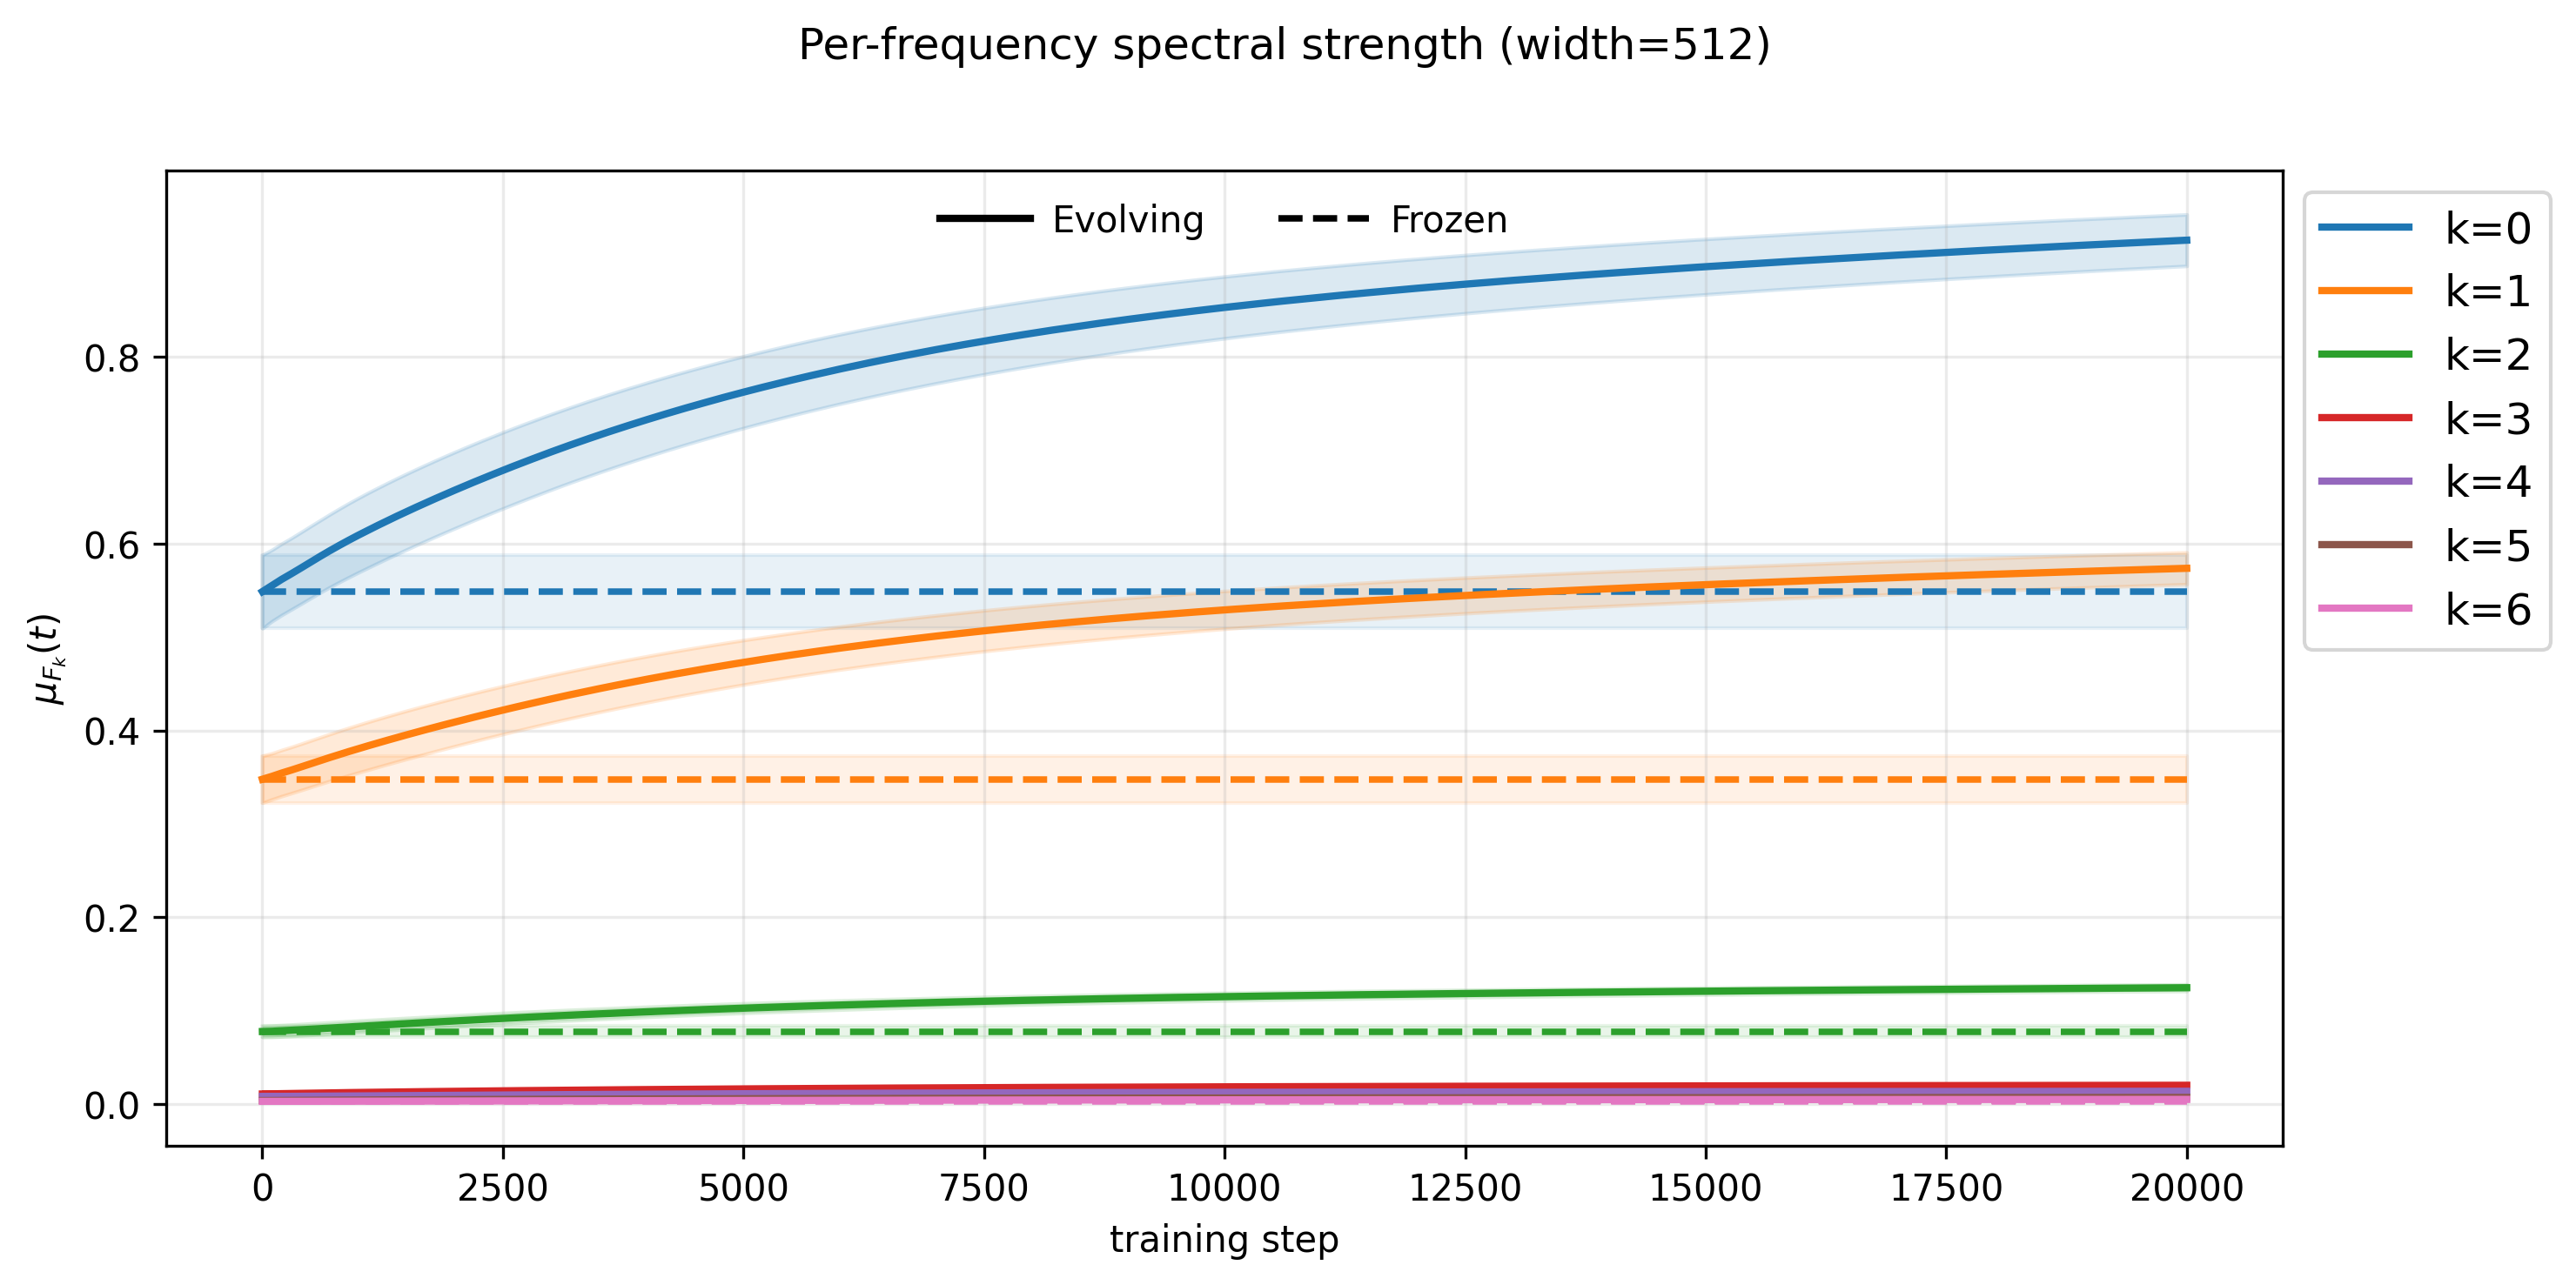
\includegraphics[width=\linewidth]{images/finite_width_evolving_results/spectral_strength_by_freq_w512.png}
		\caption{Per-frequency spectral strength.}
	\end{subfigure}

	\caption{Joint diagnostics for the evolving finite-width tangent kernel at
		width \(512\).}
	\label{fig:evolving-joint-w512}
\end{figure}

\begin{figure}[!htbp]
	\centering

	\begin{subfigure}[t]{\textwidth}
		\centering
		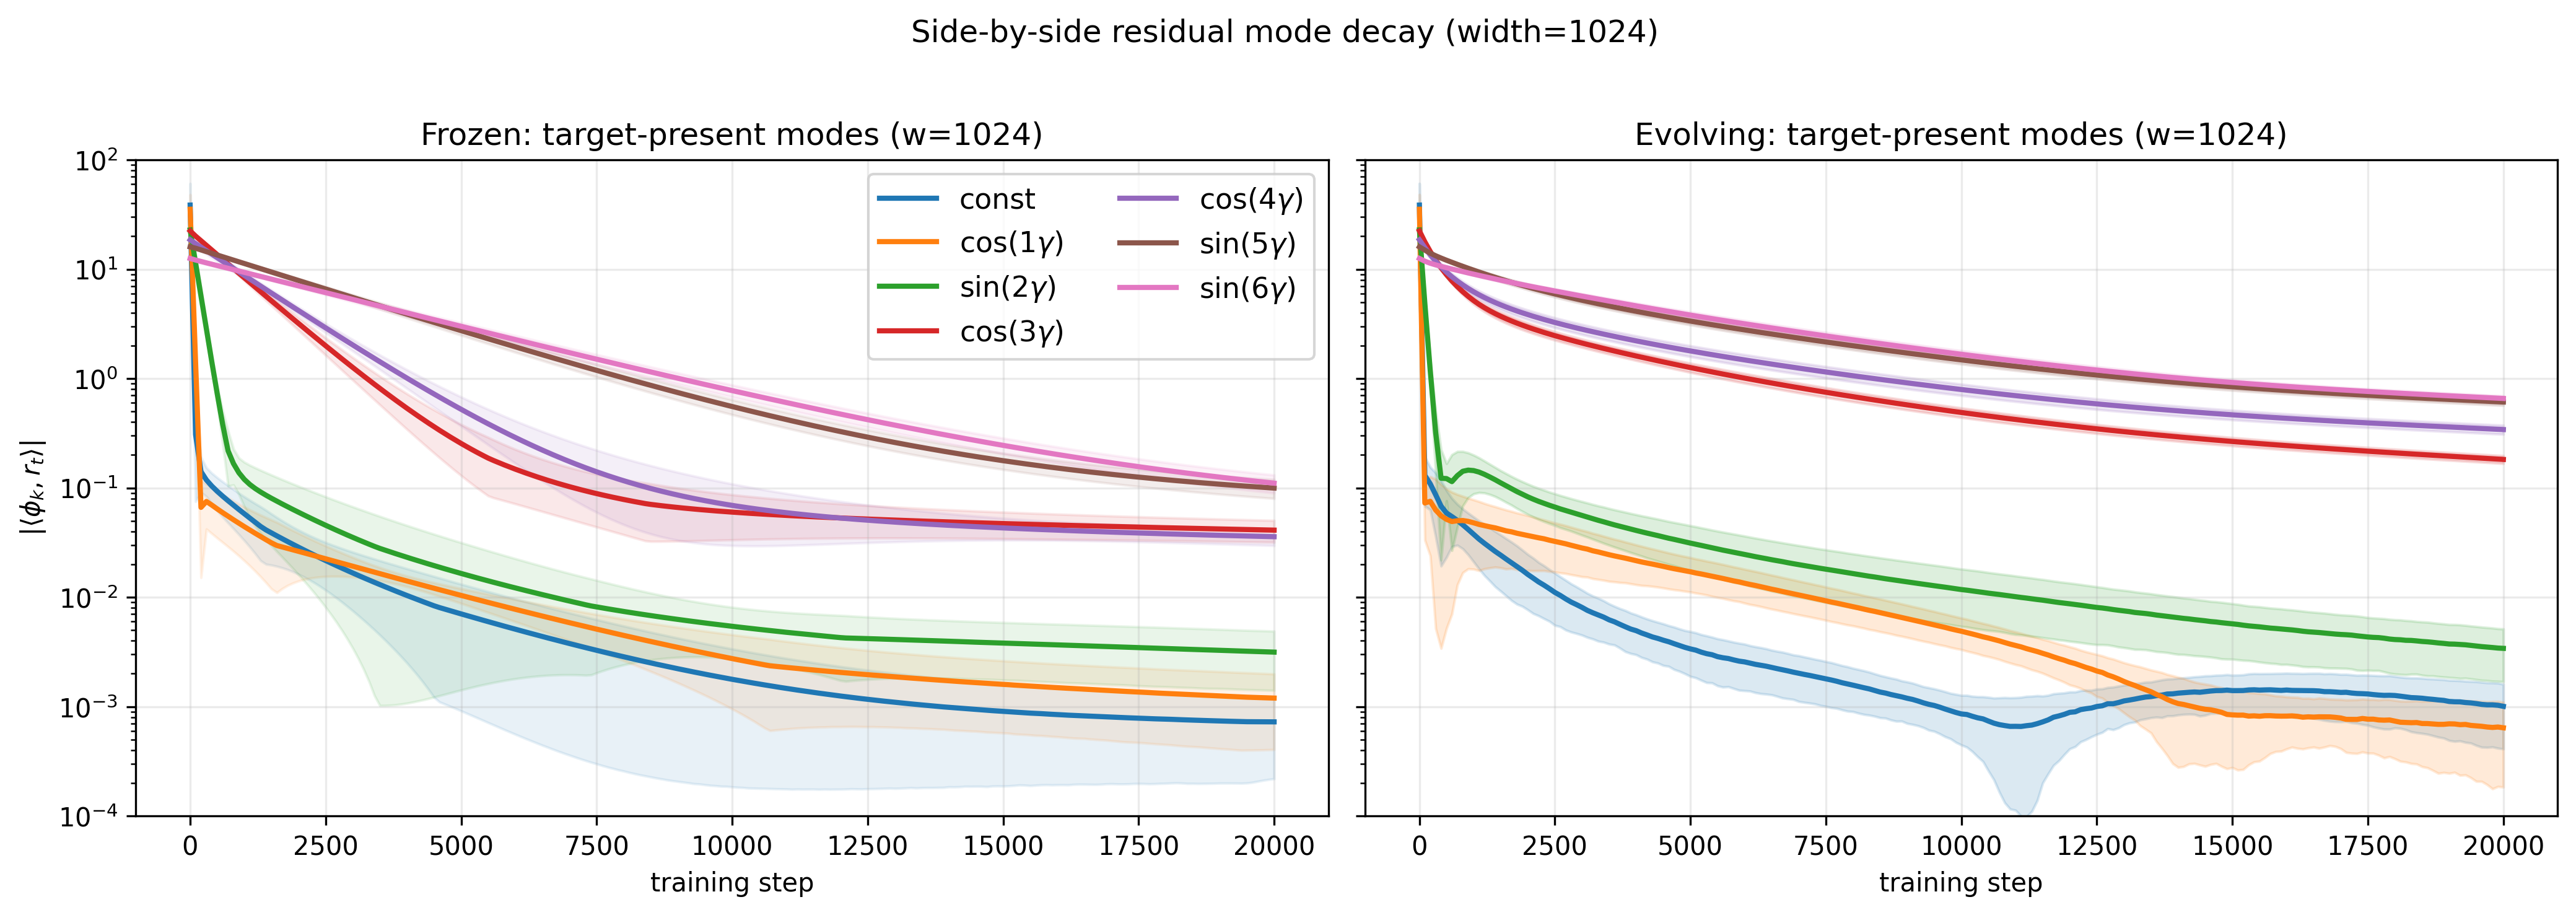
\includegraphics[width=\linewidth]{images/finite_width_evolving_results/side_by_side_residual_decay_w1024.png}
		\caption{Mode-wise residual decay.}
	\end{subfigure}

	\vspace{0.8em}

	\begin{subfigure}[t]{\textwidth}
		\centering
		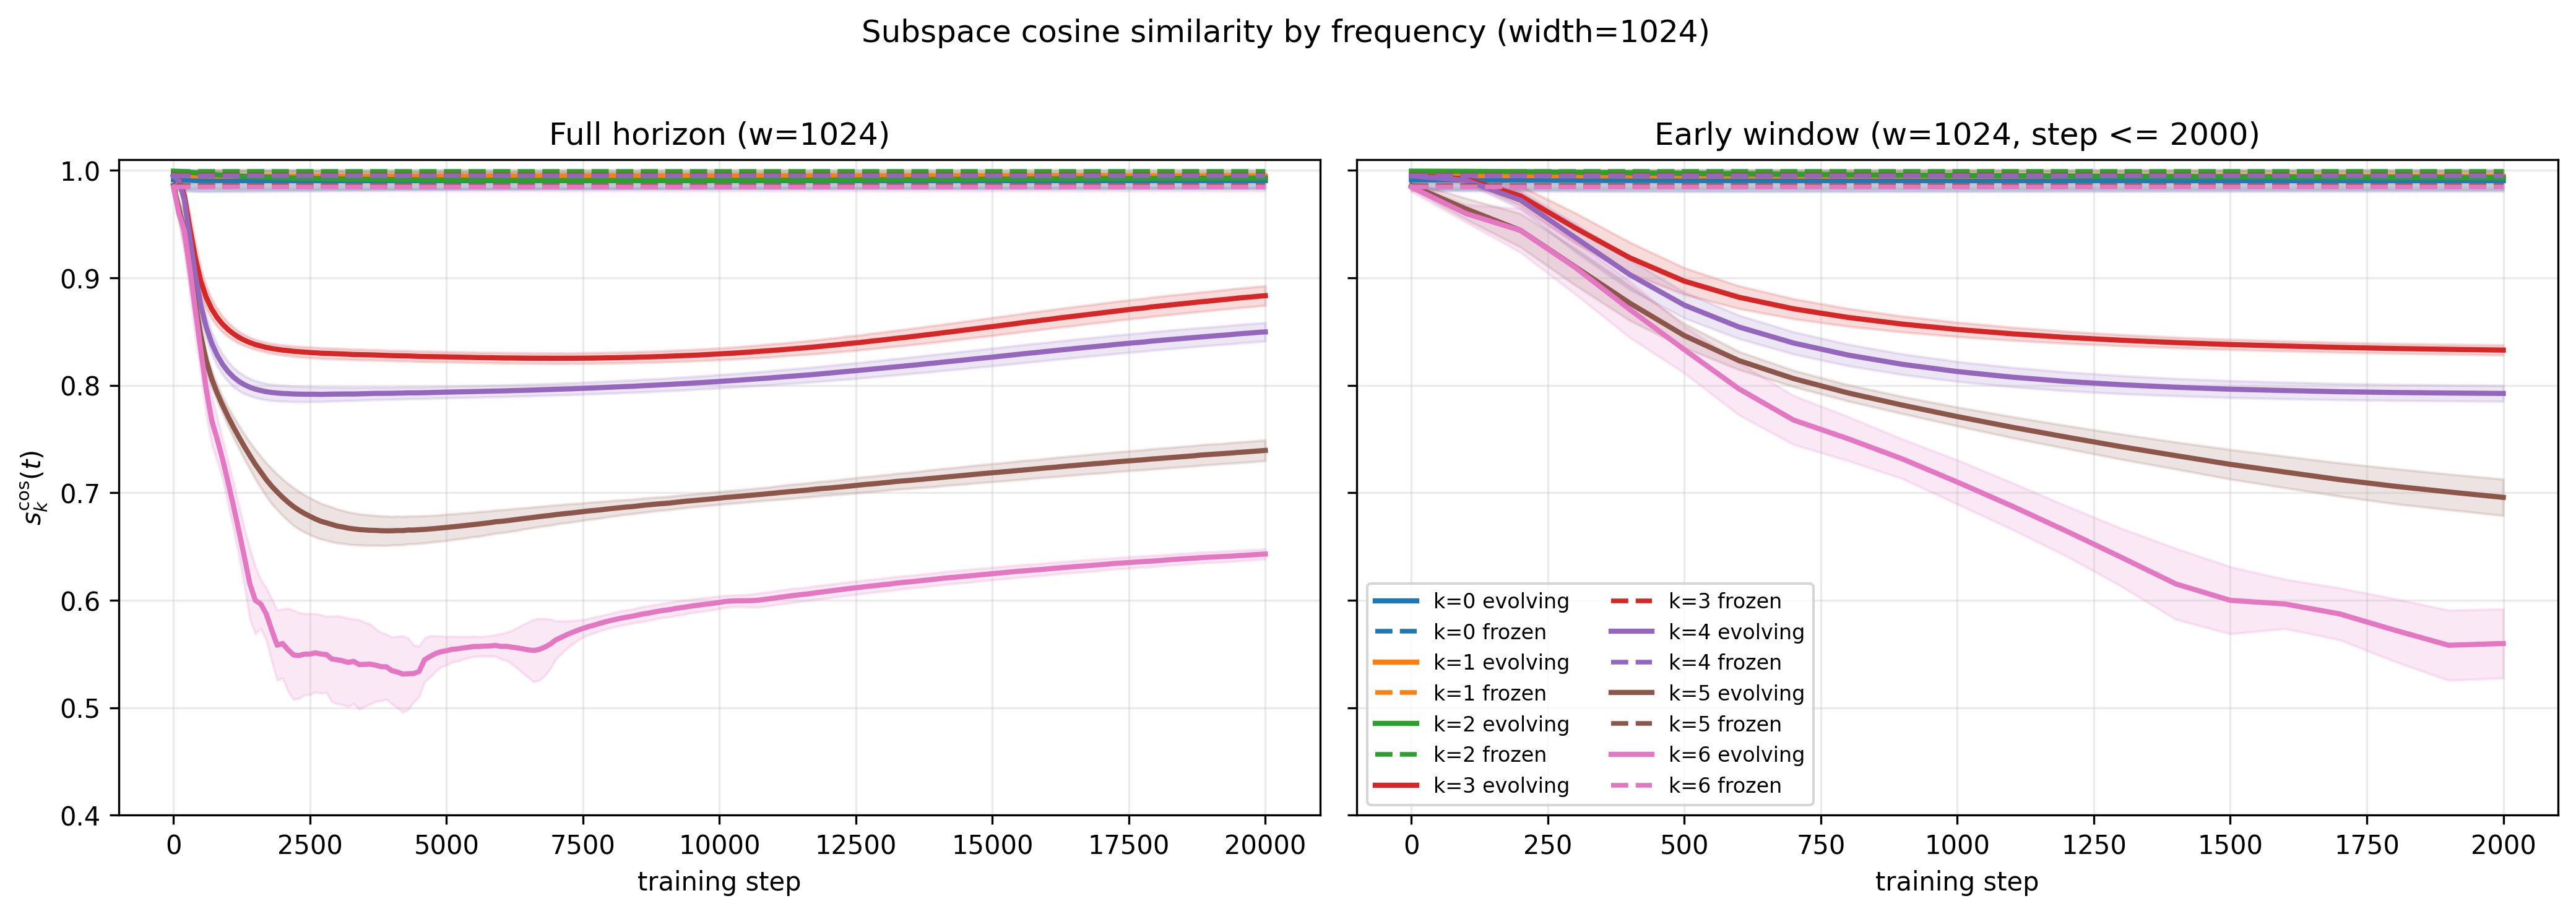
\includegraphics[width=\linewidth]{images/finite_width_evolving_results/rms_cos_alignment_by_freq_w1024.png}
		\caption{Subspace cosine similarity.}
	\end{subfigure}

	\vspace{0.8em}

	\begin{subfigure}[t]{\textwidth}
		\centering
		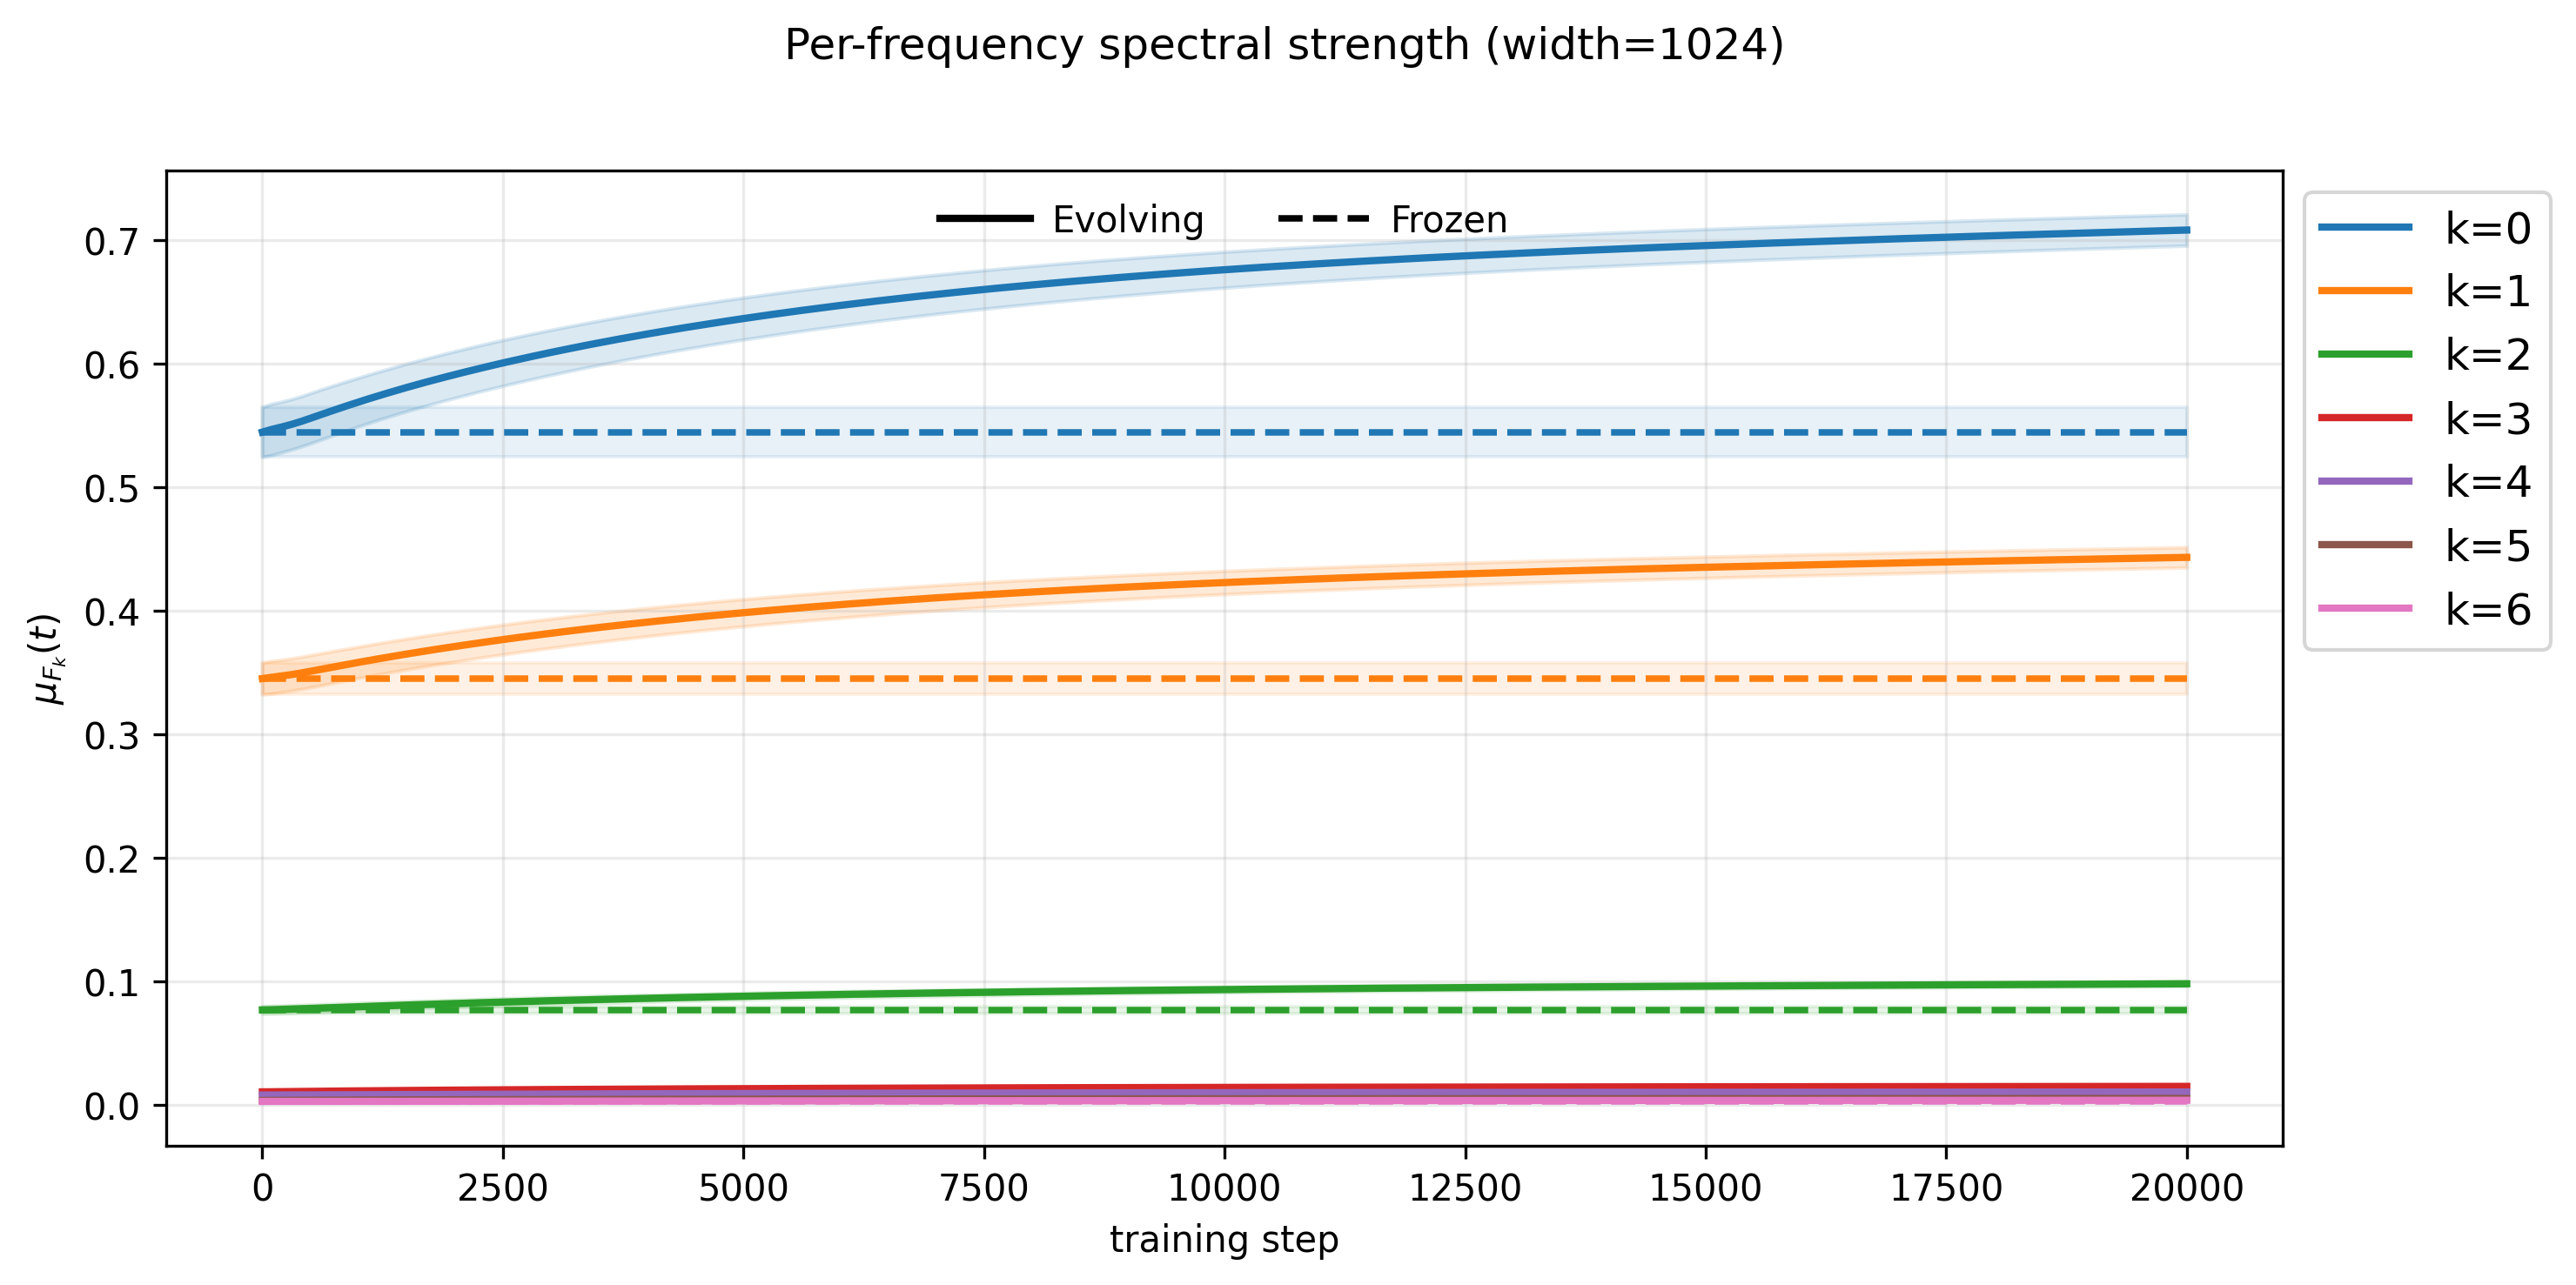
\includegraphics[width=\linewidth]{images/finite_width_evolving_results/spectral_strength_by_freq_w1024.png}
		\caption{Per-frequency spectral strength.}
	\end{subfigure}

	\caption{Joint diagnostics for the evolving finite-width tangent kernel at
		width \(1024\).}
	\label{fig:evolving-joint-w1024}
\end{figure}

Figures~\ref{fig:evolving-joint-w128}--\ref{fig:evolving-joint-w1024} show
three recurring trends. First, the mode-wise residual plots show that the early
training dynamics still largely follows the frequency ordering: lower-frequency
components decay before higher-frequency components. Kernel evolution does not
remove this ordering, but changes the relative decay rates within the retained
target modes. At widths \(128\) and \(256\), the evolving dynamics give
smaller final residuals for several low and intermediate modes, including the
constant mode, \(\cos(\varphi)\), \(\sin(2\varphi)\), \(\cos(3\varphi)\), and
\(\cos(4\varphi)\). At width \(512\), this advantage is less uniform. At width
\(1024\), the frozen dynamics are better on several components with the largest
remaining residual amplitudes, including \(\cos(3\varphi)\),
\(\cos(4\varphi)\), \(\sin(5\varphi)\), and \(\sin(6\varphi)\). Since the
least-squares objective is quadratic in the residual, these larger remaining
components have the greatest effect on the final loss.

Second, the subspace cosine similarity plots show that kernel evolution does
not improve Fourier alignment. The low-frequency subspaces, especially
\(k=0\), \(k=1\), and to a lesser extent \(k=2\), remain close to their Fourier
subspaces during training. In contrast, several higher-frequency subspaces lose
alignment early in training and only partially recover later. The frozen
alignment improves with width, as expected from the frozen finite-width results.
The evolving alignment, however, reaches a similar range across widths for some
higher frequencies. Thus, at larger width, the evolving kernel can move farther
away from the better-aligned initialization, even though the low-frequency
subspaces remain relatively stable.

Third, the spectral-strength plots show that the largest change in operator
strength occurs precisely in the low-frequency blocks that remain well aligned.
At width \(128\), the average strength in the constant block and the first
frequency increases by a large factor during training, with a smaller increase
for \(k=2\). The same effect is present at width \(256\), weaker at width
\(512\), and much smaller at width \(1024\). The higher-frequency blocks remain
weak in comparison and do not show the same increase in strength.

Taken together, these plots suggest that the small-width benefit of kernel
evolution is not caused by better preservation of Fourier geometry. The
alignment either stays similar for the lowest frequencies or worsens for higher
frequencies. The more visible effect is that kernel evolution increases the
operator strength in the low-frequency blocks that are already well aligned
with the Fourier subspaces. At small width, this extra low-frequency strength
can outweigh the loss of alignment elsewhere. At large width, the frozen kernel
already has good Fourier structure, and the additional strength gained from
kernel evolution is smaller, so the evolving dynamics no longer gives a clear
advantage.

\subsection{Width dependence of tangent-kernel drift}
\label{subsec:results-evolving-block-drift}

The previous plots compare the consequences of frozen and evolving dynamics.
We now measure the kernel movement directly. Recall from
Section~\ref{sec:finite-width-evolving-kernel-methodology} that
\[
	C_t^{(K)}=P_KT_t^{(m)}P_K
\]
denotes the low-frequency block of the finite-width tangent operator. We measure
its drift from initialization by
\[
	\|C_t^{(K)}-C_0^{(K)}\|_F .
\]

\begin{figure}[!htbp]
	\centering
	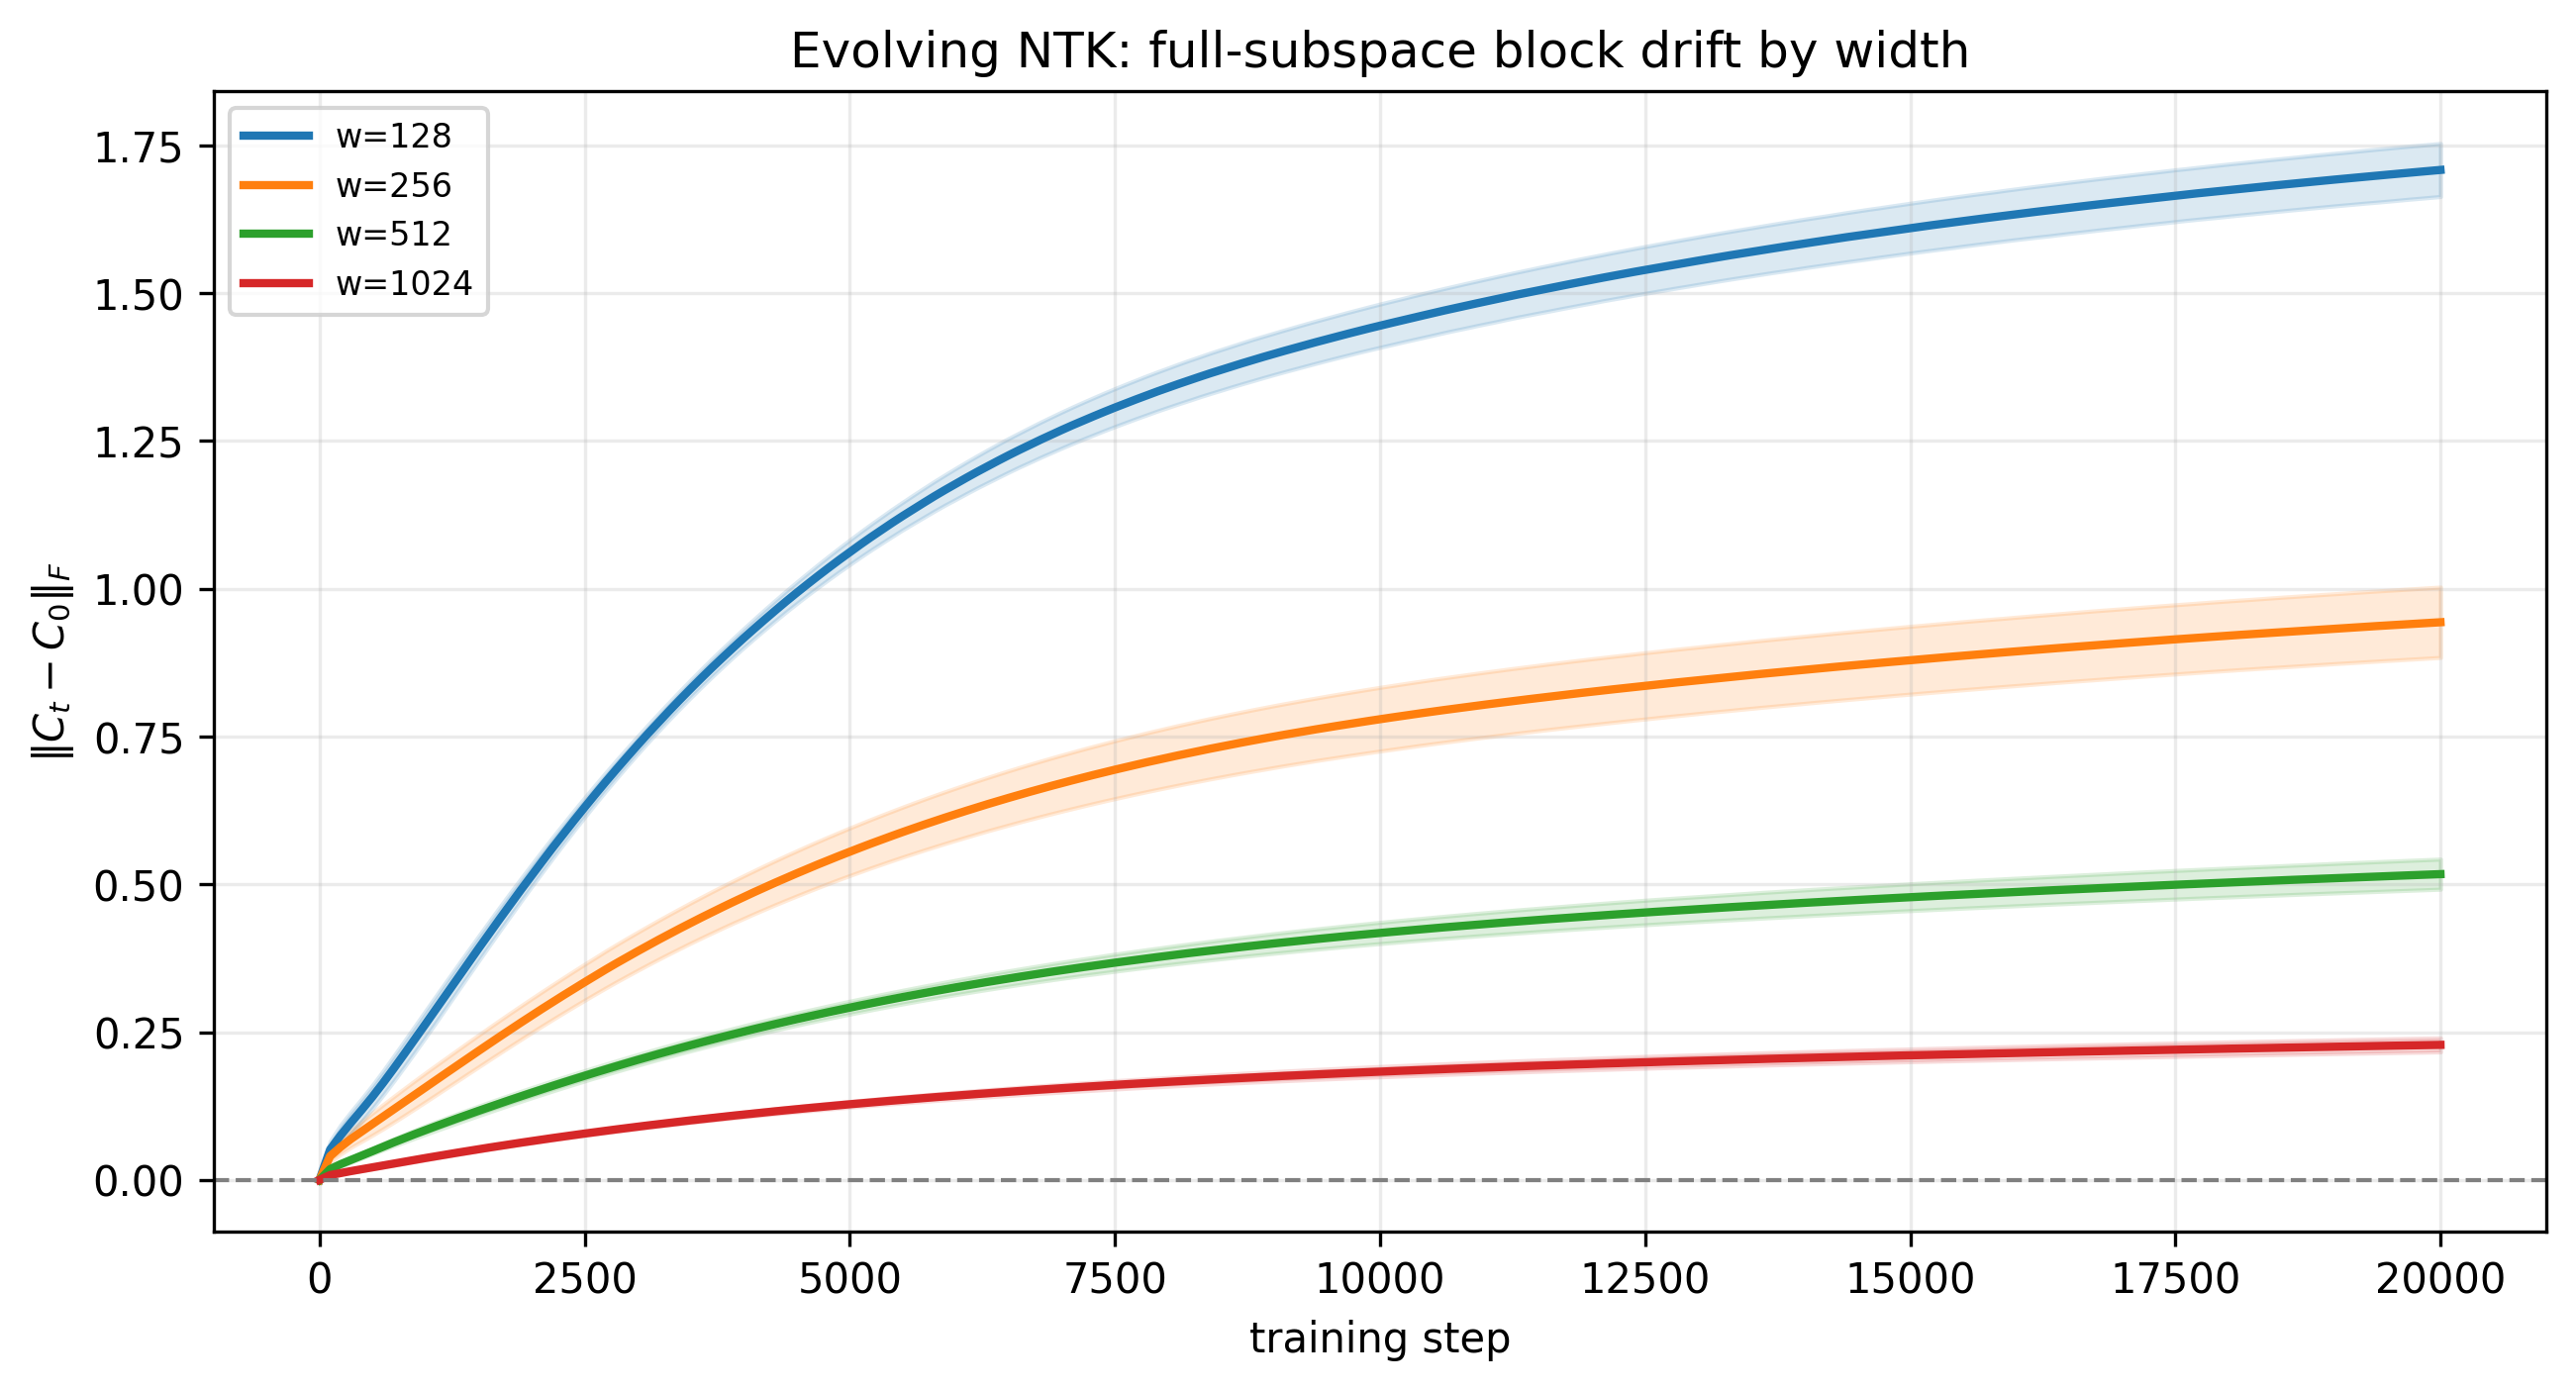
\includegraphics[width=0.9\textwidth]{images/finite_width_evolving_results/full_subspace_block_drift_fro_Ct_minus_C0_by_width_full.png}
	\caption{Drift of the projected evolving tangent-kernel block across widths,
	measured by \(\|C_t^{(K)}-C_0^{(K)}\|_F\). The low-frequency block changes
	substantially at small width and much less at larger width.}
	\label{fig:results-evolving-block-drift}
\end{figure}

Figure~\ref{fig:results-evolving-block-drift} shows the drift of the projected
low-frequency tangent block during training. The drift is largest at widths
\(128\) and \(256\), and becomes much smaller at widths \(512\) and \(1024\).
Thus, in these experiments, the finite-width tangent kernel moves less as the
width increases.

This is consistent with the NTK regime, where increasing width makes the
training dynamics closer to the linearized dynamics around initialization and
the tangent kernel changes less during training
\citep{jacot2018ntk,lee2020wide,chizat2019lazytraining}. In the present
experiments, this also explains why the difference between frozen and evolving
dynamics are most visible at small width.

\subsection{Effect of target amplitudes on spectral strength}
\label{subsec:results-evolving-amplitude-variants}

The spectral-strength plots above suggest that the evolving tangent kernel
increases its strength mainly on the low-frequency blocks. One possible concern
is that this effect could be caused by the particular amplitudes in the target
function. In the original target, the lower-frequency components have larger
amplitudes than the higher-frequency components. To check whether the observed
spectral reweighting is tied to this choice, we repeat the evolving-kernel
experiment with two modified targets.

The three targets are
	{\footnotesize
		\begin{align}
			f_{\mathrm{orig}}(\gamma)
			 & =
			1.0
			+0.9\cos(\gamma)
			-0.8\sin(2\gamma)
			+0.7\cos(3\gamma)
			+0.6\cos(4\gamma)
			-0.5\sin(5\gamma)
			-0.4\sin(6\gamma),
			\label{eq:results-target-original}
			\\
			f_{\mathrm{eq}}(\gamma)
			 & =
			1.0
			+\cos(\gamma)
			-\sin(2\gamma)
			+\cos(3\gamma)
			+\cos(4\gamma)
			-\sin(5\gamma)
			-\sin(6\gamma),
			\label{eq:results-target-equalamp}
			\\
			f_{\mathrm{rev}}(\gamma)
			 & =
			0.4
			+0.5\cos(\gamma)
			-0.6\sin(2\gamma)
			+0.7\cos(3\gamma)
			+0.8\cos(4\gamma)
			-0.9\sin(5\gamma)
			-\sin(6\gamma).
			\label{eq:results-target-revamp}
		\end{align}
	}

The equal-amplitude target gives all active non-constant modes the same
amplitude. The reversed-amplitude target gives the largest amplitudes to the
higher-frequency modes.

\begin{figure}[!htbp]
	\centering
	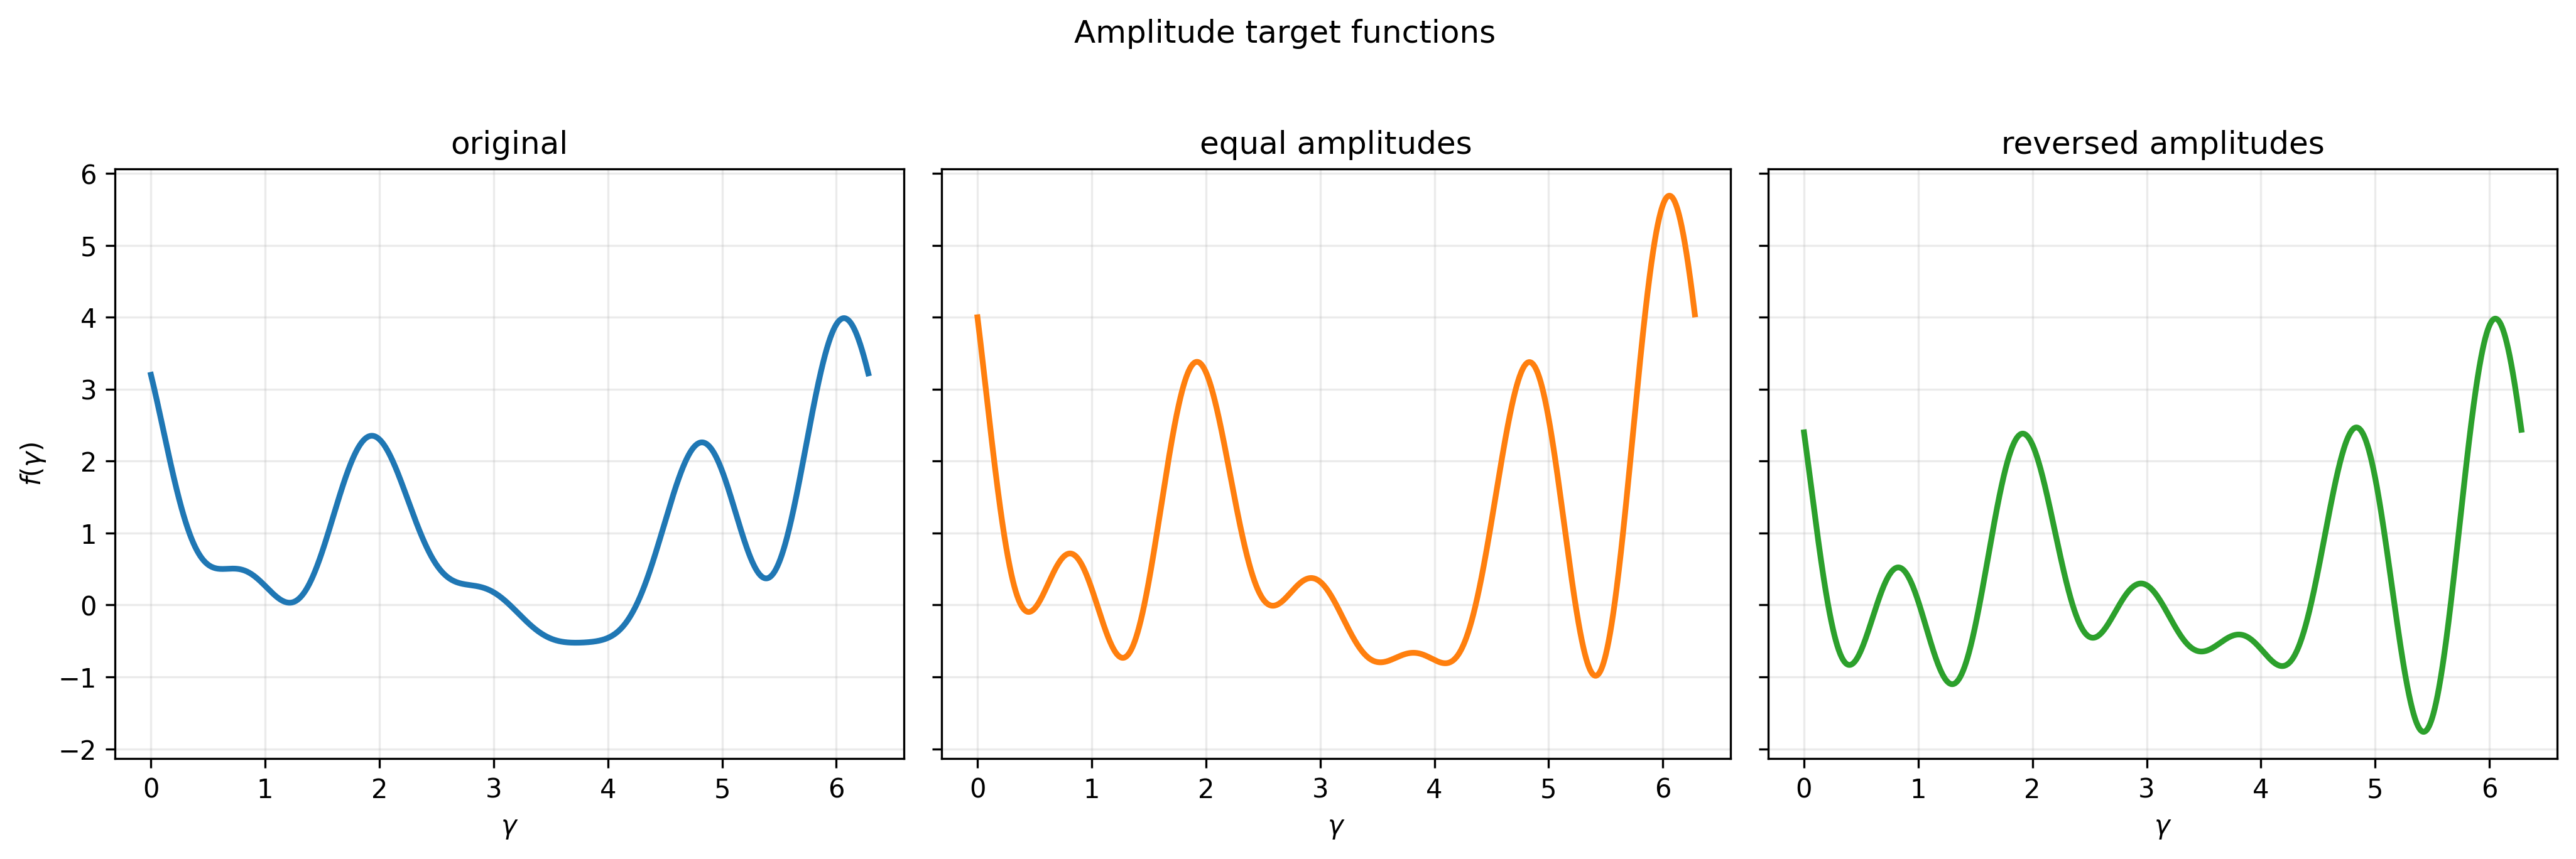
\includegraphics[width=\textwidth]{images/finite_width_evolving_results/amplitude_target_functions.png}
	\caption{Target functions used in the amplitude-variant experiments. The
		original target has larger amplitudes on lower frequencies, the
		equal-amplitude target assigns the same amplitude to all active
		non-constant modes, and the reversed-amplitude target gives larger
		amplitudes to higher frequencies.}
	\label{fig:results-amplitude-target-functions}
\end{figure}

\begin{figure}[!htbp]
	\centering

	\begin{subfigure}[t]{0.48\textwidth}
		\centering
		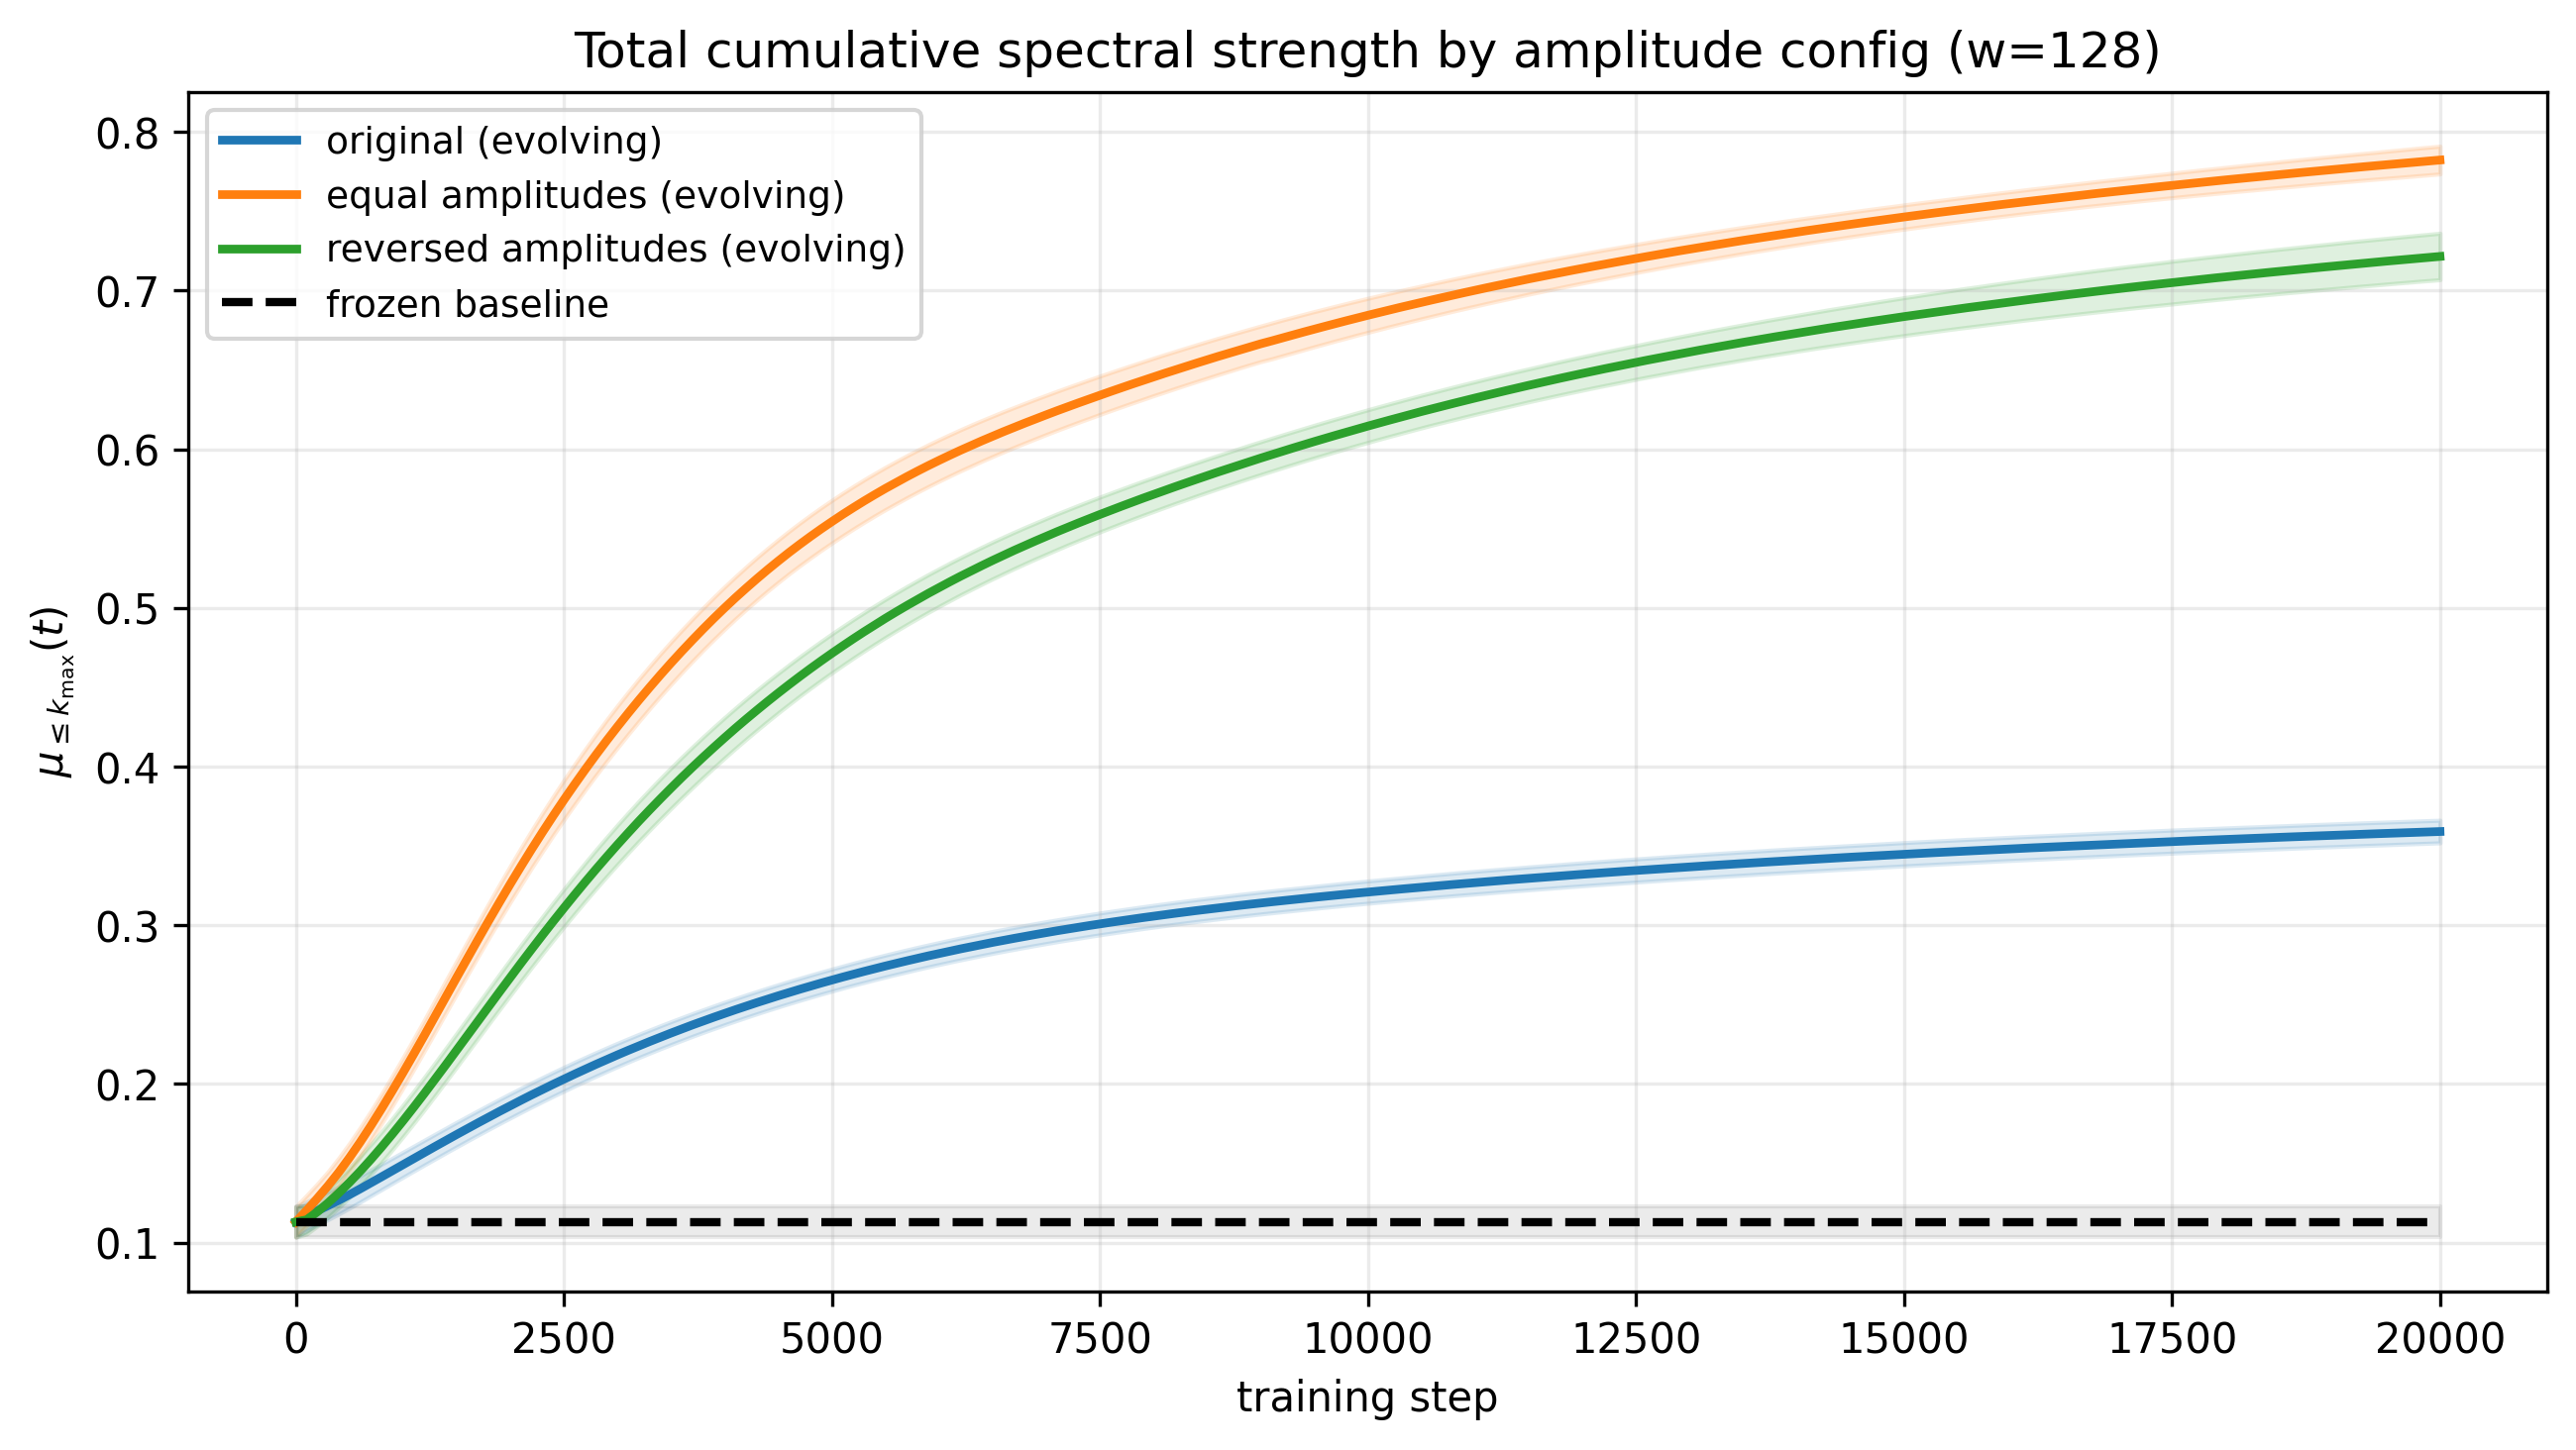
\includegraphics[width=\linewidth]{images/finite_width_evolving_results/total_cumulative_mu_amp_configs_w128.png}
		\caption{\(w=128\).}
	\end{subfigure}
	\hfill
	\begin{subfigure}[t]{0.48\textwidth}
		\centering
		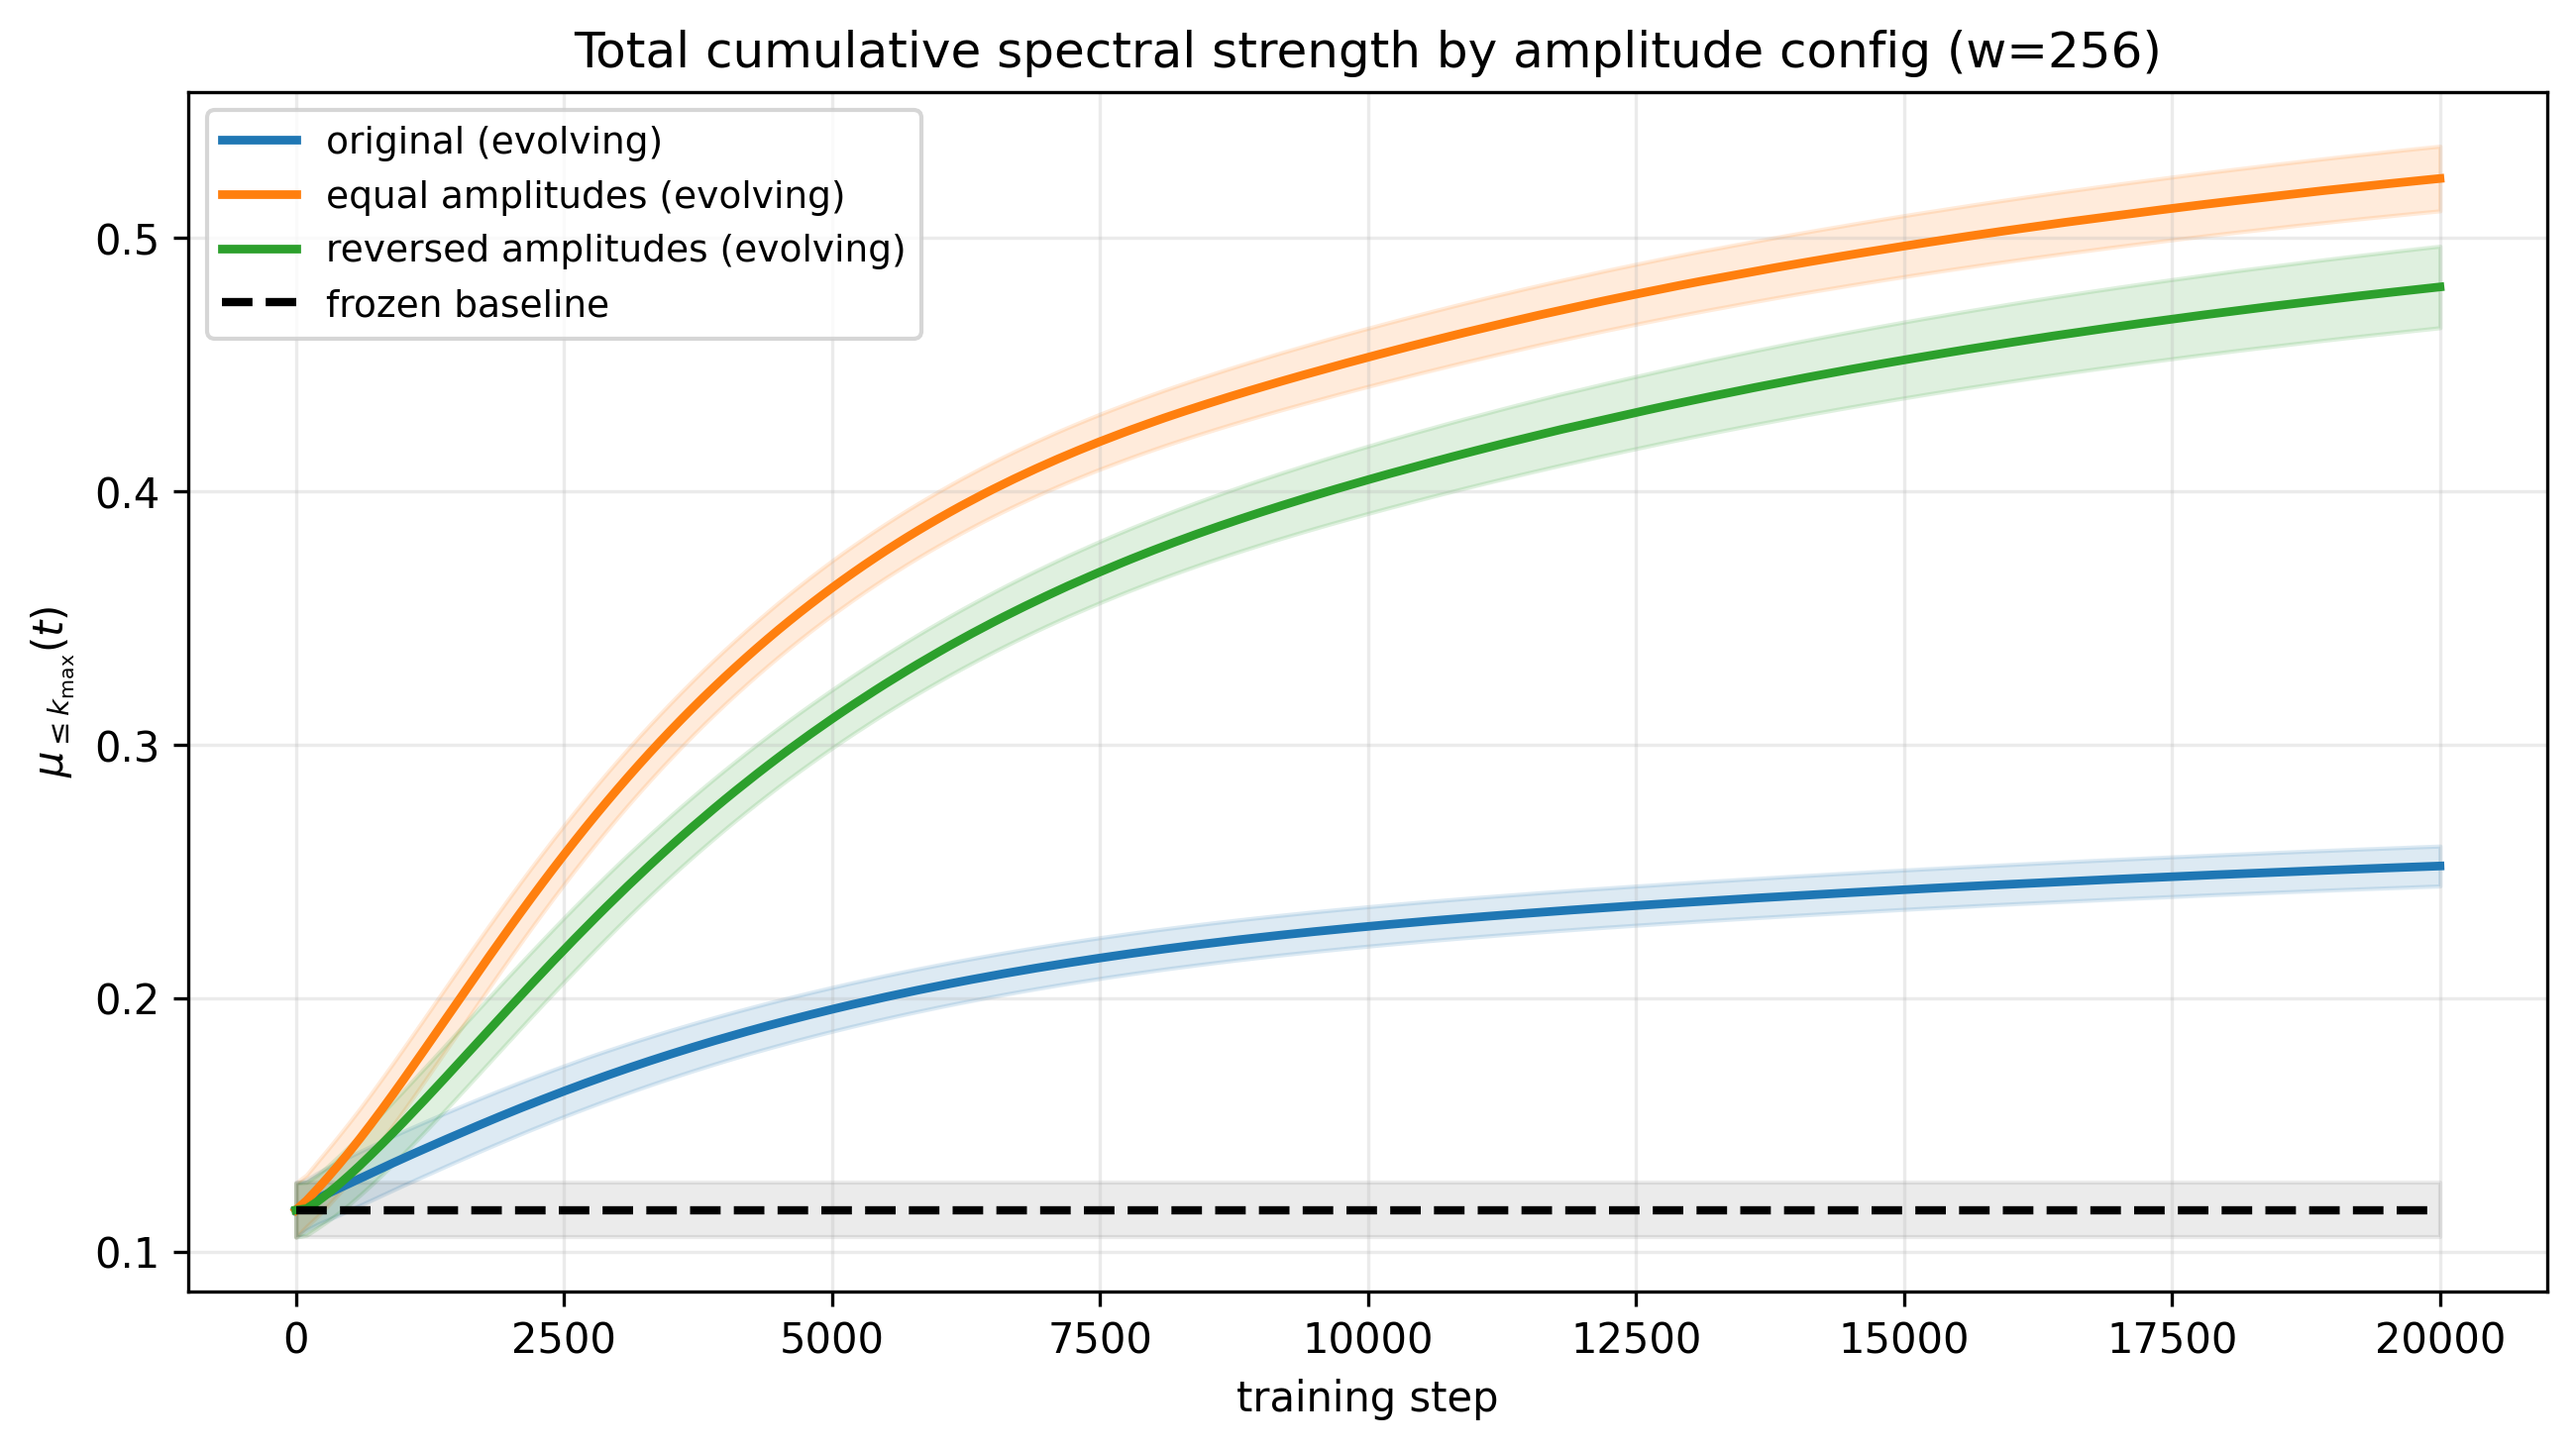
\includegraphics[width=\linewidth]{images/finite_width_evolving_results/total_cumulative_mu_amp_configs_w256.png}
		\caption{\(w=256\).}
	\end{subfigure}

	\vspace{0.8em}

	\begin{subfigure}[t]{0.48\textwidth}
		\centering
		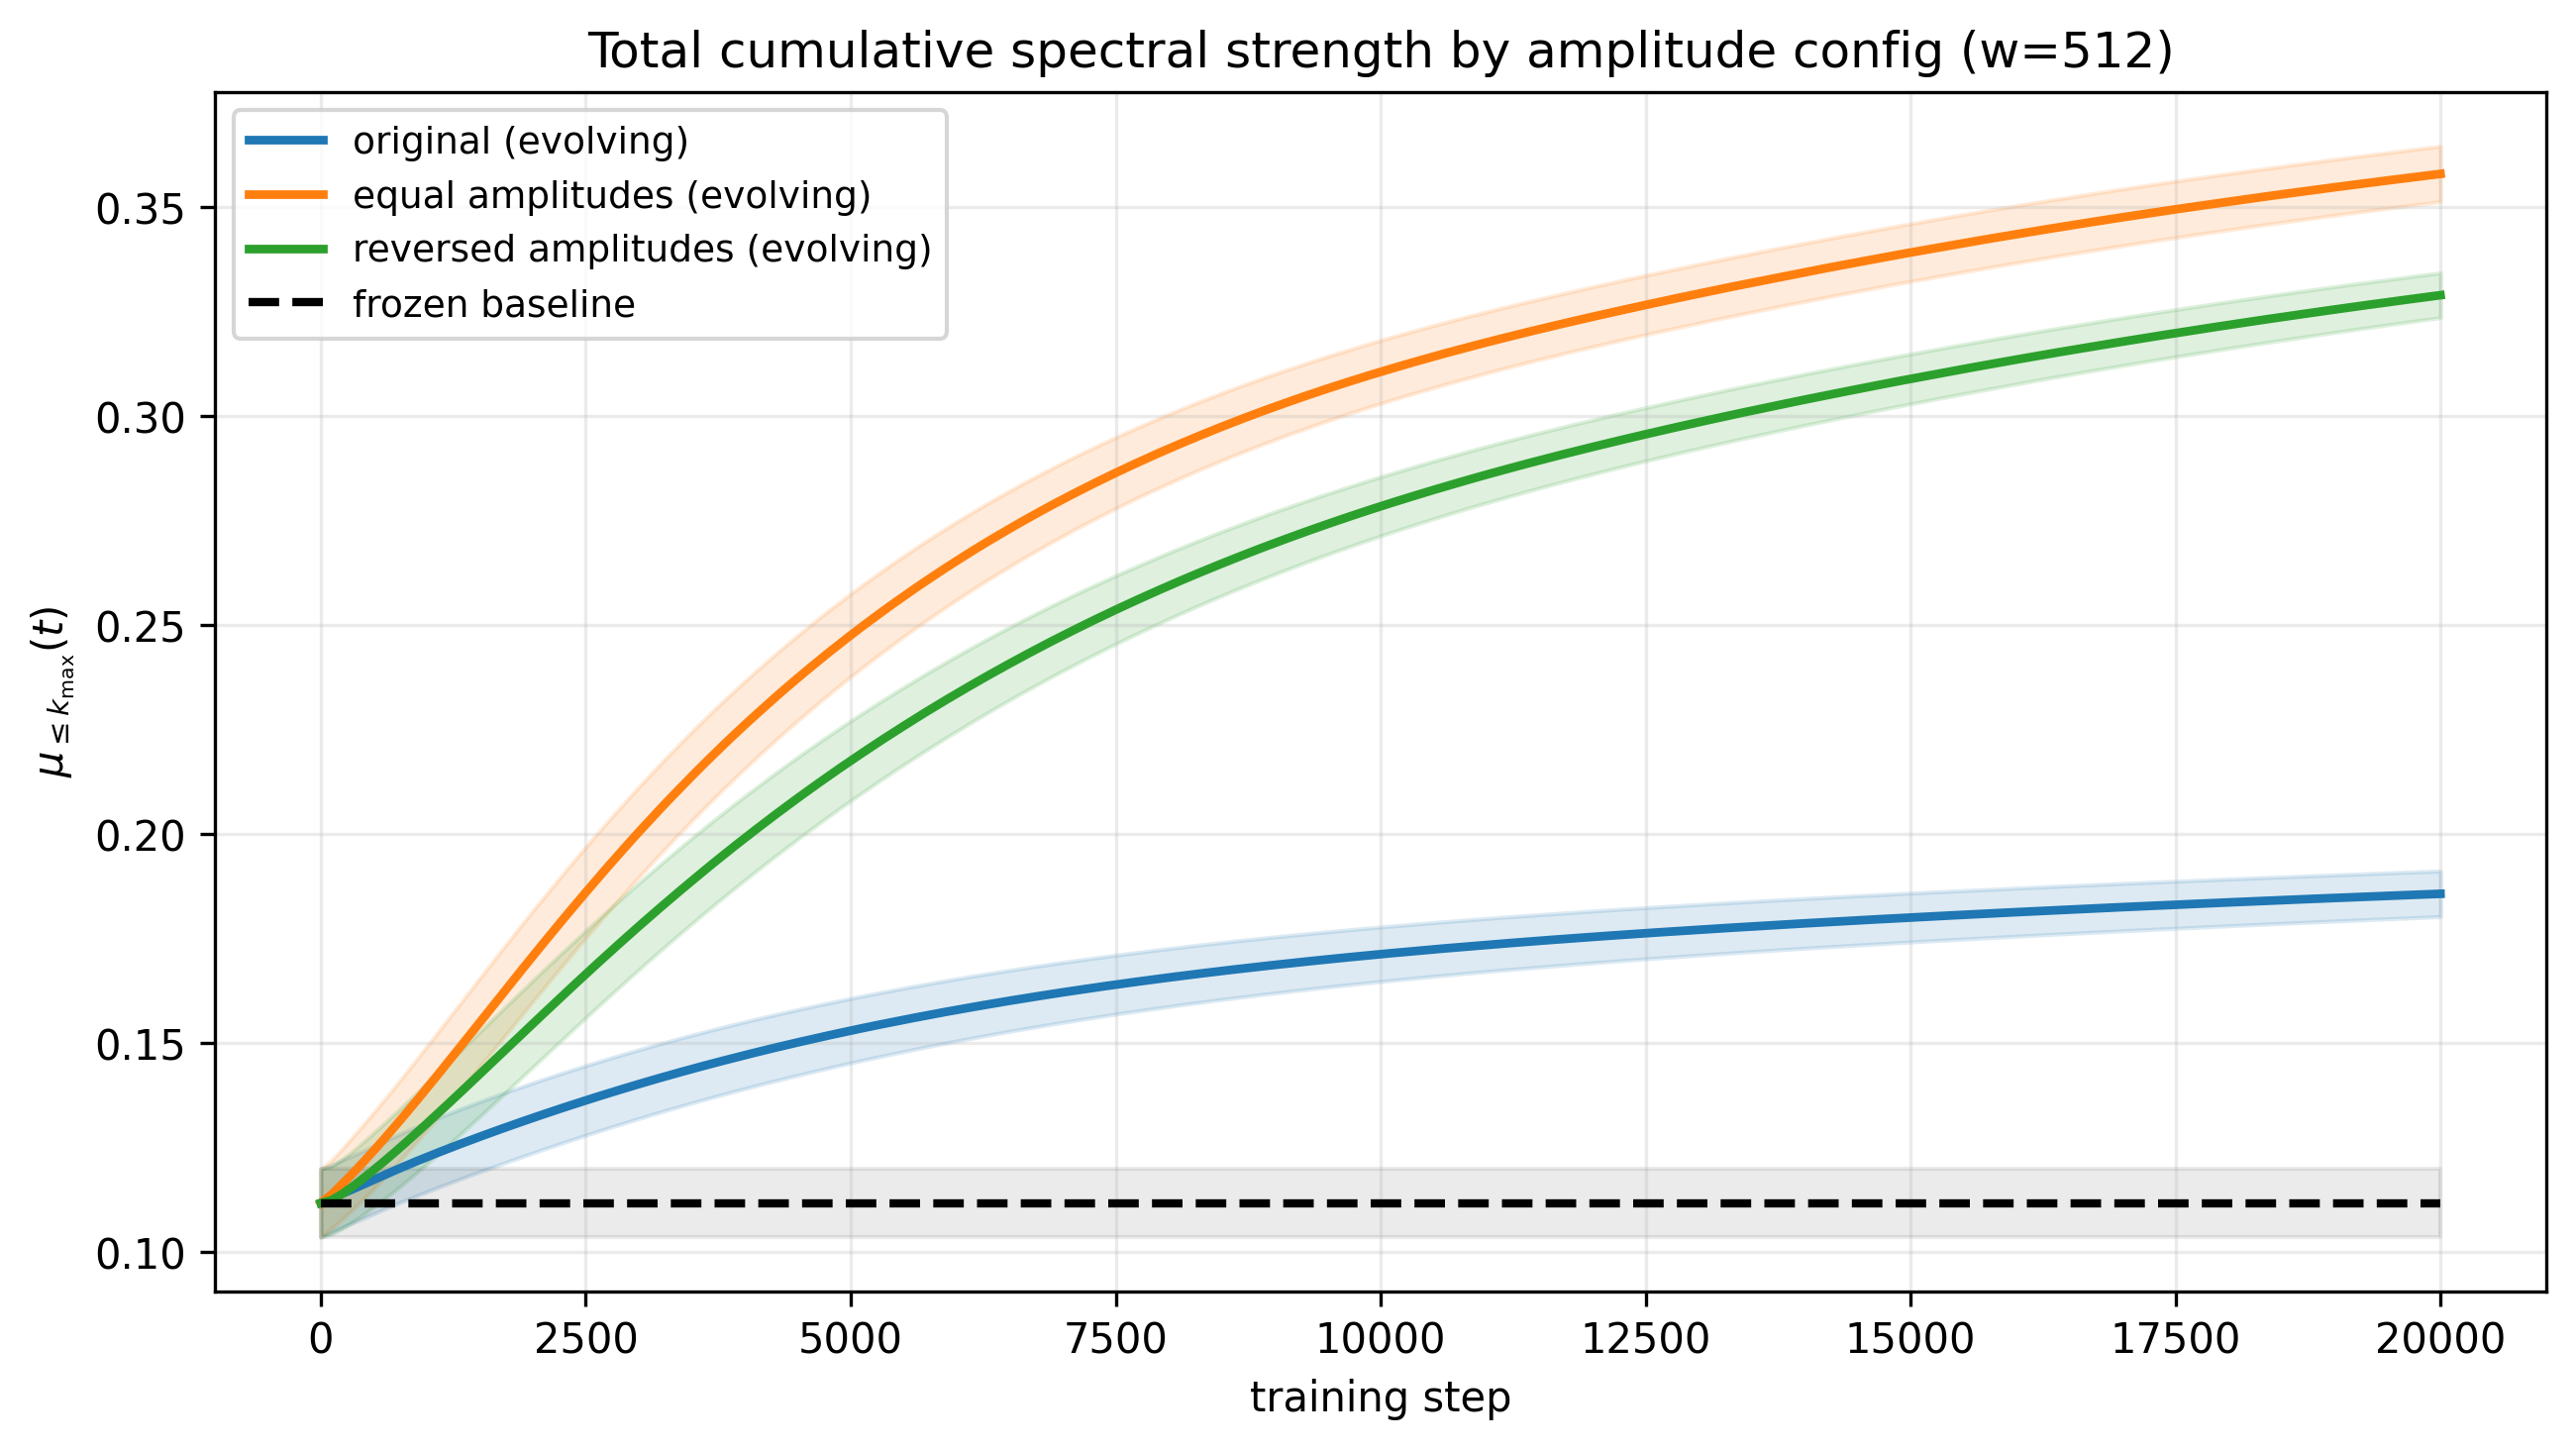
\includegraphics[width=\linewidth]{images/finite_width_evolving_results/total_cumulative_mu_amp_configs_w512.png}
		\caption{\(w=512\).}
	\end{subfigure}
	\hfill
	\begin{subfigure}[t]{0.48\textwidth}
		\centering
		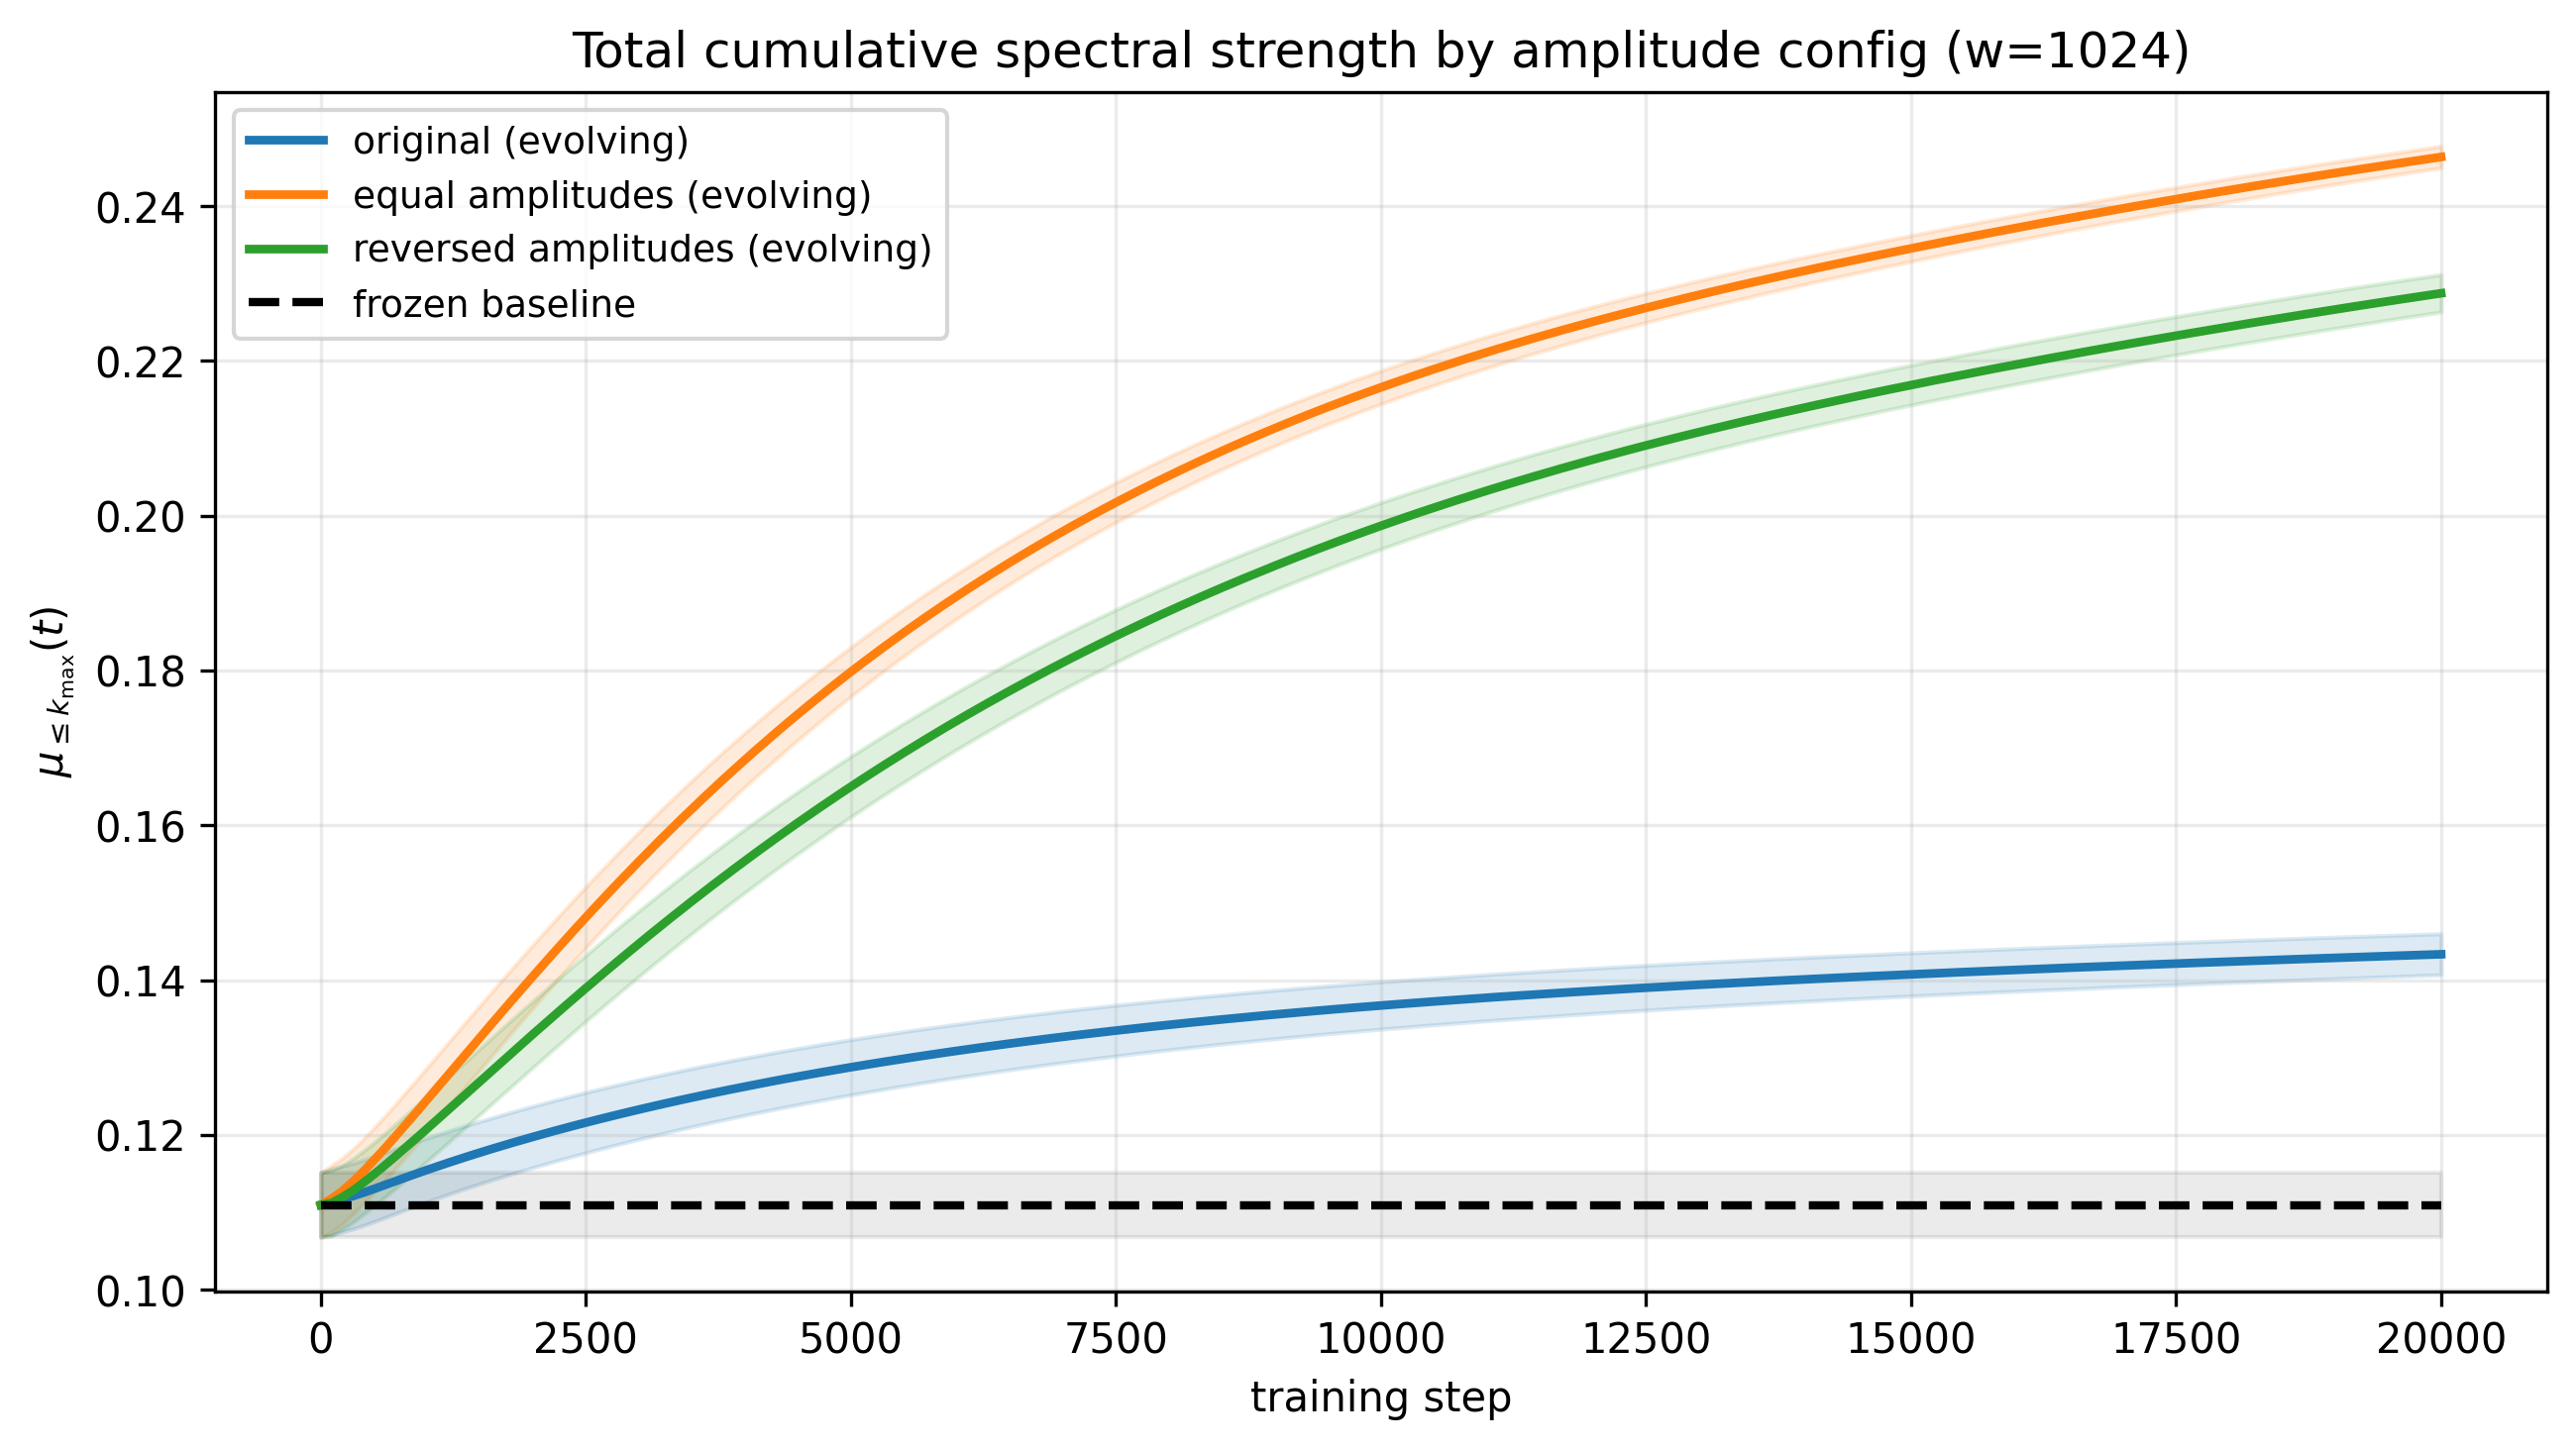
\includegraphics[width=\linewidth]{images/finite_width_evolving_results/total_cumulative_mu_amp_configs_w1024.png}
		\caption{\(w=1024\).}
	\end{subfigure}

	\caption{Cumulative low-frequency spectral strength under different target
		amplitude choices. The dashed line shows the frozen baseline, while the
		solid curves show the evolving tangent kernel for the original,
		equal-amplitude, and reversed-amplitude targets.}
	\label{fig:results-cumulative-strength-amplitude-variants}
\end{figure}

Figure~\ref{fig:results-cumulative-strength-amplitude-variants} shows that the
increase in cumulative spectral strength is not specific to the original target
amplitudes. For all widths, the evolving tangent kernel increases the average
strength on the retained low-frequency block relative to the frozen baseline.
This increase is largest for the equal-amplitude target, smaller but still clear
for the reversed-amplitude target, and weakest for the original target.

The effect also decreases with width. At width \(128\), all evolving curves move
well above the frozen baseline. At width \(1024\), the same ordering is still
visible, but the increase is smaller. Thus, the low-frequency strength increase
persists across all three amplitude choices. It is not only a consequence of
the original target assigning larger amplitudes to lower frequencies: the
increase is also present when all non-constant modes have equal amplitudes, and
when the larger amplitudes are assigned to higher frequencies.

The ordering across targets is also worth noting. In these experiments, the
equal-amplitude target produces the largest increase, the reversed-amplitude
target produces a smaller but still clear increase, and the original target
produces the weakest increase. In particular, the reversed-amplitude target
still produces a larger low-frequency strength increase than the original
target, despite putting larger amplitudes on higher-frequency modes.

\section{Summary of results}
\label{sec:results-summary}

This chapter tested how the idealized infinite-width, infinite-data spectral
bias picture changes under realistic constraints in a controlled fashion.
Throughout these analyses, the primary comparisons are made on the retained
low-frequency subspace $\mathcal{H}_K$, which contains the constant mode and
the first $K$ non-zero Fourier frequencies.

The core findings are:

\begin{itemize}
	\item \textbf{Ideal continuum setting:} Under the limiting NTK, each
	      Fourier component evolves independently. Lower frequencies possess larger
	      eigenvalues and decay faster. Crucially, the architecture dictates the
	      spectrum: odd modes $k \ge 3$ only receive non-zero eigenvalues if the
	      network includes a trainable hidden bias.

	\item \textbf{Finite sampling:} Replacing the continuous measure with $n$
	      discrete samples destroys exact Fourier diagonalization. However, on
	      $\mathcal{H}_K$, the sampled operator deviates from the ideal Fourier
	      prediction by an error of just $O(n^{-1/2})$ (with fixed confidence, up to
	      logarithmic factors). The corrected finite-sample eigenvalues (see
	      ~\ref{prop:results-expectation-H}) accurately predict the dominant
	      early-time residual decay.

	\item \textbf{Frozen finite width:} When fixing a finite-width ($m$)
	      tangent kernel at initialization, it acts as a random perturbation of the
	      continuum operator. On $\mathcal{H}_K$, the projected finite-width operator
	      concentrates around the infinite-width baseline at a rate of $O(m^{-1/2})$.

	\item \textbf{Evolving finite width:} Allowing the kernel to train
	      empirically breaks the fixed-kernel assumption. At small widths, training
	      alters the operator to actively increase low-frequency spectral strength
	      (particularly for $k=0$ and $k=1$). This advantage diminishes at larger
	      widths, where the frozen initialization is already tightly concentrated
	      around the ideal baseline.
\end{itemize}

\chapter{Discussion and conclusion}
\label{cha:discussion-conclusion}

On the circle \(S^1\), functions can be decomposed into sine and cosine waves, i.e. the Fourier basis.
This makes the circle a useful setting for studying spectral bias. Low
frequencies describe slowly varying structure, while high frequencies describe
more oscillatory structure. The question is whether the training dynamics treat
these components differently, and whether this distinction remains meaningful
after moving away from the ideal infinite-width and infinite-data setting.

In the continuum infinite-width reference model, the answer is explicit. The
limiting NTK is rotation-invariant, so the associated operator is diagonal in
the Fourier basis. Each Fourier component of the residual evolves independently:
\begin{equation}
	\alpha_p(t)
	=
	\exp(-\lambda_p t)\alpha_p(0),
	\label{eq:discussion-continuum-mode-decay}
\end{equation}
where \(\alpha_p(t)\) is the residual coefficient of the \(p\)-th Fourier basis
function, and \(\lambda_p\) is the corresponding kernel eigenvalue. For the
ReLU NTK studied here, the low-frequency eigenvalues are larger, so the
low-frequency residual components decay faster. This gives the fixed-kernel
spectral-bias mechanism in this setting
\citep{jacot2018ntk,lee2020wide,rahaman2019spectralbiasneuralnetworks,
	basri2019convergence,bietti2019inductivebiasneuraltangent,
	cao2020understandingspectralbiasdeep}.

The continuum calculation also shows the importance of including a trainable hidden bias in the
network. With the hidden-bias contribution, odd frequencies \(k\ge 3\) have
nonzero eigenvalues. Without this contribution, those frequencies are null
directions of the fixed-kernel dynamics. Thus, the architecture itself
affects whether some frequencies are learned at all by the fixed-kernel
operator.

\section{RQ1: Finite sampling}
\label{sec:discussion-finite-sampling}

The first research question asked what happens when the uniform continuum
measure on \(S^1\) is replaced by finitely many sampled input points.

Exact Fourier-wise learning is lost after sampling. The sampled sine and cosine
vectors are not exactly orthonormal, and they are not exact eigenvectors of the
sampled NTK operator. However, on any fixed low-frequency block
\begin{equation}
	\mathcal H_K
	=
	\operatorname{span}\{1,\cos(\varphi),\sin(\varphi),\ldots,
	\cos(K\varphi),\sin(K\varphi)\},
	\label{eq:discussion-low-frequency-block}
\end{equation}
this error decreases as the number of samples increases. At fixed confidence,
the typical finite-sample error is of order \(n^{-1/2}\), up to logarithmic
factors.

This means that the Fourier picture survives as an approximation, not as an
exact statement. The finite-sample corrected eigenvalues describe the dominant
early-time dynamics of the retained Fourier components. Later in training, some
components have already become very small. At that point, the remaining
finite-sample error can become visible relative to the component being plotted.
This explains why the empirical curves can deviate from the ideal prediction at
late times without contradicting the finite-sample theory.

The preconditioning experiment supports the same interpretation. If the
different decay rates are mainly caused by the Fourier eigenvalues, then
rescaling by those eigenvalues should remove much of the separation between the
retained components. This is what is observed. The experiment therefore acts as
a check that the rate separation is mostly explained by the predicted spectrum,
rather than by an unrelated numerical artifact.

The answer to the first research question is therefore that finite sampling does
not preserve exact Fourier diagonalization, but it preserves it approximately on
fixed low-frequency blocks. The approximation improves with sample size, and it
is strong enough to explain the leading residual dynamics seen in the
experiments.

\section{RQ2: Finite width}
\label{sec:discussion-finite-width}

The second research question asked what happens when the network has finite
width. There are two distinct cases. In the frozen-kernel case, the tangent
kernel is sampled at initialization and then kept fixed. In the evolving-kernel
case, the tangent kernel changes during training.

For the frozen tangent kernel, finite width behaves like a random perturbation
of the infinite-width operator. On the fixed low-frequency space
\(\mathcal H_K\), the projected finite-width operator concentrates around the
continuum operator at rate \(m^{-1/2}\), up to logarithmic factors. The
eigenspace experiments show the same effect geometrically: as width increases,
the finite-width eigenspaces become better aligned with the corresponding
Fourier frequency subspaces.

The approximation is not equally stable for every frequency. Low frequencies
have larger eigenvalues, so a small perturbation has less relative effect on
their dynamics. Higher frequencies have smaller eigenvalues and smaller gaps
between nearby eigenvalues, so the same perturbation can be more visible. This
matches the broader spectral-bias picture: high-frequency components are learned
later and are more sensitive to details of the model and data distribution
\citep{rahaman2019spectralbiasneuralnetworks,basri2019convergence,
	basri2020frequencybiasneuralnetworks}.

The evolving-kernel case is different. Here the fixed-kernel explanation is no
longer complete, because the operator itself changes during training. The
results in this part are empirical rather than theorem-level statements.

At small widths, allowing the kernel to evolve improves the final loss. At
larger widths, this advantage becomes smaller and eventually disappears. The
measurements suggest that the improvement is not caused by better alignment with
the Fourier subspaces. Several higher-frequency subspaces become less aligned
during training. Instead, the main visible change is that the evolving kernel
increases the average operator strength in the lowest Fourier blocks, especially
\(k=0\) and \(k=1\), with a smaller increase for \(k=2\). This agrees with the
residual plots, where the strongest improvements occur in low and intermediate
target components.

The amplitude-variant experiments make this interpretation less dependent on
the particular target used in the main experiment. The same low-frequency
strength increase appears when all active non-constant modes have equal
amplitudes, and also when larger amplitudes are assigned to higher frequencies.
This suggests that the effect is not simply caused by the original target having
larger low-frequency coefficients.

The answer to the second research question is therefore split. For frozen finite
width, the continuum Fourier picture remains approximately valid when the width
is large. For evolving finite width, the Fourier subspaces remain useful as
diagnostics, but the fixed-kernel picture no longer fully explains the dynamics.
Training can reshape the tangent kernel, and this can change the effective
learning rates of different frequency components.

\section{Main conclusion}
\label{sec:discussion-main-conclusion}

The main research question asked whether the continuum infinite-width Fourier
description survives under finite sampling and finite width.

For finite sampling, it survives approximately on fixed low-frequency blocks.
The sampled operator is not exactly diagonal in the Fourier basis, but the error
decreases with the number of samples, and the corrected eigenvalues explain the
dominant early-time residual dynamics.

For frozen finite width, it also survives approximately. The finite-width
operator is random at initialization, but its projection onto \(\mathcal H_K\)
concentrates around the continuum operator as the width increases.

For evolving finite width, the Fourier description changes role. It is no
longer a complete dynamical explanation, because the kernel is not fixed. It is
instead a useful coordinate system for measuring how training changes the
operator. In the experiments here, the most important change is an increase in
low-frequency operator strength at small width.

Thus, finite sampling and frozen finite width behave like controlled
perturbations of the ideal NTK model on fixed low-frequency blocks. Kernel
evolution adds a separate effect: training can modify the operator itself, and
this can make the finite-width network behave differently from its frozen
kernel approximation.

\section{Limitations}
\label{sec:discussion-limitations}

The concentration results are fixed-block results. They control a prescribed
low-frequency space \(\mathcal H_K\) with fixed \(K\). They do not give a
uniform statement over all Fourier modes, and they are not designed to remain
sharp when \(K\) grows with \(n\) or \(m\). This matters because higher
frequencies have smaller eigenvalues and narrower eigengaps. Controlling more
frequencies would require more accurate operator approximations.

The bounds are also conservative. The proofs use entrywise concentration and
union bounds over the retained block. These arguments are enough to prove the
correct decreasing trends, but they discard matrix structure and variance
information. This explains why the theoretical bounds are much larger than the
observed numerical errors. Sharper estimates would likely require direct
operator-norm bounds, variance-sensitive concentration, or tools for U- and
V-statistics.

The finite-sample theory explains the leading behaviour of the sampled
fixed-kernel dynamics, but it does not give a sharp time-uniform description of
every residual component. Once a component has decayed close to zero, small
operator errors can dominate the plotted quantity. The current bounds explain
why such deviations should occur, but they do not predict the exact level of
each late-time deviation.

The finite-width theorem controls the frozen tangent kernel at initialization.
It does not control the evolving tangent kernel during training. The
evolving-kernel experiments show a consistent pattern, but they do not establish
a theorem for the time-dependent operator. A rigorous explanation would need to
control how the tangent kernel moves and how this movement interacts with the
current residual.

The alignment diagnostics also have a limited interpretation. Projector errors
and principal angles measure how close empirical eigenspaces are to Fourier
subspaces, but they do not by themselves determine the loss dynamics. Loss decay
depends on how the current operator acts on the current residual. This is why
worse Fourier alignment can coexist with lower loss when the evolving kernel
also increases operator strength in important directions.

Finally, the thesis does not prove a joint theorem combining finite sampling,
finite width, and training time. The finite-sample and frozen finite-width
analyses isolate separate perturbations of the continuum operator. Actual finite
training runs contain sampling error, finite-width randomness, and kernel
evolution at the same time.

\section{Beyond the uniform circle setting}
\label{sec:discussion-beyond-uniform-circle}

The Fourier basis is the right reference in this thesis because the domain is
the circle and the input distribution is uniform. These assumptions make the
limiting kernel rotation-invariant, so the associated operator is diagonalized
by sine and cosine functions.

For non-uniform input densities, the Fourier basis should not be expected to
remain the exact reference. The relevant operator is weighted by the input
density, and its eigenfunctions need not be global Fourier modes. In that case,
spectral bias should be understood more generally as a preference for the
leading eigenfunctions of the kernel operator induced by the architecture and
the data distribution
\citep{basri2020frequencybiasneuralnetworks,
	bowman2022spectralbiasoutsidetraining}. These eigenfunctions may correspond
to smooth variation along the data distribution, rather than low frequency in
the usual Fourier sense.

For other domains, the same idea applies. On higher-dimensional spheres, the
analogues of Fourier modes are spherical harmonics. On less symmetric domains,
there may be no closed-form eigensystem. The operator viewpoint still applies,
but the preferred directions may be much harder to describe explicitly.

Changing the activation function would also change the kernel spectrum. With an
isotropic initialization on the uniform circle, activations such as sigmoid or
tanh may still produce rotation-invariant kernels, so the Fourier basis may
remain an eigenbasis. However, the eigenvalues would change. A smoother
activation can produce a smoother kernel, which may make high-frequency
eigenvalues decay faster. Polynomial activations can behave differently again,
because they may only activate finitely many harmonic components. Thus spectral
bias is not independent of the activation. It depends on the spectrum of the
kernel generated by the architecture, parameterization, and data distribution.

The role of bias terms may also change. In the ReLU model studied here, the
trainable hidden bias supplies nonzero eigenvalues to odd modes \(k\ge 3\).
For another activation or parameterization, the same odd-even structure need not
hold. The broader point is that architecture can affect not only the speed of
learning different components, but also which components are visible to the
fixed-kernel dynamics.

Moving away from the NTK parameterization would change the interpretation even
more. The fixed-kernel limit is tied to the NTK scaling. In feature-learning or
mean-field regimes, the representation can move substantially during training,
so a fixed initial kernel cannot be expected to describe the full dynamics
\citep{Mei2018meanfieldview,chizat2018globalconvergencegradientdescent}. In
such regimes, the natural object is no longer only the spectrum at
initialization, but the evolution of the operator or of the parameter
distribution during training.

\section{Future work}
\label{sec:discussion-future-work}

The most direct next step is to develop theory for the evolving finite-width
tangent kernel. The experiments in this thesis compare frozen and evolving
dynamics, but the evolving-kernel analysis remains empirical. A natural goal is
to control the time-dependent low-frequency block, its drift from
initialization, and its effect on the residual dynamics.

A second direction is to prove a joint result for finite sampling, finite width,
and training time. This would better match actual training runs, where all three
effects occur together.

A third direction is to sharpen the concentration bounds. The current proofs are
sufficient to show decreasing error with \(n\) and \(m\), but they are not
numerically sharp. Direct operator-norm concentration, variance-sensitive
estimates, or concentration inequalities for U- and V-statistics may give bounds
closer to the observed errors.

A fourth direction is to study the alignment diagnostics more directly. The
projector-error and principal-angle plots suggest that different Fourier
subspaces have different finite-width stability. A more detailed analysis could
measure which Fourier blocks are most strongly mixed by the finite-width
operator and how this depends on eigenvalues and eigengaps.

Finally, the analysis should be extended beyond the uniform circle. Non-uniform
densities, higher-dimensional domains, other activations, and different
parameterizations all change the relevant kernel operator and its spectrum.
Studying these cases would clarify which conclusions are special to the explicit
Fourier model on \(S^1\), and which reflect a broader mechanism behind spectral
bias.

\section{Conclusion}
\label{sec:discussion-final-conclusion}

This thesis studied spectral bias in a setting where the ideal training dynamics
can be written explicitly. On the uniform circle, the infinite-width NTK is
diagonal in the Fourier basis. Each frequency has its own learning rate, and low
frequencies are learned faster because they correspond to larger kernel
eigenvalues.

The results show that this picture is stable under finite sampling and frozen
finite width, as long as one works on a fixed low-frequency block. In both
cases, the ideal Fourier operator is perturbed, but the perturbation decreases
with sample size or width. The evolving finite-width experiments show where the
fixed-kernel explanation stops being complete. When the kernel moves during
training, the Fourier basis remains useful for measurement, but the dynamics are
also shaped by how the operator itself changes.

The final picture is therefore simple. The Fourier basis is exact in the
continuum reference model. It remains approximately valid for finite sampling
and frozen finite width. For evolving finite width, it becomes a diagnostic for
understanding how training reshapes the kernel. Turning this last observation
into a theorem is the main open problem left by this work.

\chapter{Use of Generative AI}\label{cha:genai}

In accordance with the TU Delft guidelines on the use of generative AI in
end projects, I disclose here the tools used in preparing this thesis, their
purpose, and the scope of their application. All ideas, research directions,
calculations, and theorems in this work are my own: the derivations were
carried out manually and double-checked with professors who are experts in the
relevant fields, and generative AI was used only as a supporting aid that I
reviewed and verified at every stage. Concretely, ChatGPT~5.3 Thinking was used for
brainstorming and for organizing my thoughts into actionable plans, and ChatGPT
Codex~5.3 assisted with coding tasks such as setting up and running experiments
and debugging. Generative AI also assisted in writing the scripts used to
produce the plots in this thesis; these scripts were subsequently read and
adjusted manually to ensure correctness. For the written text, large language
model tools were used to improve grammar, spelling, and clarity, to smooth
transitions between sections, and to make the document more coherent. My
handwritten derivations were converted into \LaTeX{} with the help of tools such
as Mathpix and LLM-based assistants (ChatGPT, Gemini), which were also used to
improve the consistency of notation throughout; the underlying mathematics is
my own. Finally, NotebookLM was used as a retrieval system to quickly locate
specific claims within the literature for citation; I read all cited papers
myself, and this tool served purely for convenient lookup. In all cases I retain
full creative and intellectual responsibility for the content, results, and
academic integrity of this thesis, and I have verified the accuracy, validity,
and originality of all material included.


\bibliographystyle{apalike}
\bibliography{bibliography/thesis}

\appendix
\def\chaptername{Appendix}
\chapter{Mean-Field Viewpoint}
\label{cha:mean-field-appendix}

The main text uses the NTK viewpoint as its main analytical framework because
it gives a fixed operator on functions. On \(S^1\), this operator can be
diagonalized in the Fourier basis, which makes it possible to discuss
frequency-dependent learning in terms of eigenvalues and eigenspaces.

The mean-field viewpoint gives another way to take a large-width limit. It is
not used in the main finite-sample or finite-width analysis, but it is useful
context because it describes a different aspect of wide-network training. In
the mean-field scaling, one does not primarily track a fixed tangent kernel at
initialization. Instead, one tracks how the hidden neurons are distributed in
parameter space, and how this distribution changes during training.

This appendix records the corresponding derivation for a two-layer network. The
purpose is to keep the comparison available without interrupting the main line
of the thesis.

\section{\label{app:mf-overview}Overview and relation to the NTK viewpoint}

Consider a two-layer network with the mean-field scaling
\begin{equation}
	f_\theta(x)
	=
	\frac{1}{m}
	\sum_{\alpha=1}^m
	v_\alpha\,\varphi(w_\alpha^\top x).
	\label{eq:app-mf-network-overview}
\end{equation}
Here each neuron has parameters
\[
	\theta_\alpha=(v_\alpha,w_\alpha)
	\in
	\Omega:=\mathbb R\times\mathbb R^d .
\]
The key observation is that the network output depends on the collection of
neurons only through their empirical distribution,
\[
	\mu_m
	:=
	\frac{1}{m}
	\sum_{\alpha=1}^m \delta_{\theta_\alpha}.
\]
Indeed,
\[
	f_\theta(x)
	=
	\int_\Omega v\,\varphi(w^\top x)\,d\mu_m(v,w).
\]
Thus the state of the network can be described by a probability measure over
neuron parameters.

In suitable large-width limits, the empirical measure \(\mu_m\) converges to a
deterministic time-dependent measure \(\mu_t\). Training is then described by
the evolution of this measure. This viewpoint was developed for two-layer
networks by \citet{Mei2018meanfieldview}, and related interacting-particle
descriptions were studied by \citet{Rotskoff_2022}. From an optimization
perspective, \citet{chizat2018globalconvergencegradientdescent} studied the
corresponding many-particle limit using tools from optimal transport.
Extensions and rigorous frameworks for deeper networks have also been studied
\citep{nguyen2019meanfieldlimitlearning,araujo2019meanfieldlimitcertaindeep,
	sirignano2019meanfieldanalysisneural,nguyen2023rigorousframeworkmeanfield}.

This viewpoint is useful because it can describe feature movement in the
large-width limit. In contrast, the strict NTK limit freezes the tangent kernel:
the features defined by the gradients at initialization remain fixed in the
limit. For the spectral question studied in this thesis, however, the NTK
viewpoint is more directly useful. The main object here is an operator on
functions whose eigenvalues and eigenspaces can be compared with Fourier modes
on \(S^1\). The mean-field viewpoint instead describes the evolution of a
probability measure over parameters, so it does not give a single fixed
Fourier-diagonal operator in the same way.

\section{\label{app:mf-detailed}Detailed derivation of the mean-field representation}

\section{\label{app:mf-detailed}Detailed derivation of the mean-field representation}

\subsection{\label{app:mf-empirical-measure}Parameter space and empirical measure}

Let $\Omega := \mathbb{R} \times \mathbb{R}^d$
denote the parameter space, and let $\mathcal{F}$ be its Borel $\sigma$-algebra.
For each neuron $\alpha$, define the Dirac measure $\delta_{\theta_\alpha}$ on
$(\Omega,\mathcal{F})$, i.e. if $A \in \mathcal{F}$ then,
\[
	\delta_{\theta_\alpha}(A)
	=
	\begin{cases}
		1, & \theta_\alpha \in A, \\
		0, & \text{otherwise}.
	\end{cases}
\]
Define the empirical neuronal measure
\begin{equation}
	\mu_m := \frac{1}{m}\sum_{\alpha=1}^m \delta_{\theta_\alpha}.
	\label{eq:app-empirical-measure}
\end{equation}
By construction, $\mu_m \ge 0$ and  $\mu_m(\Omega)=1$, hence $\mu_m \in
	\mathcal P(\Omega)$ where $\mathcal P(\Omega)$ is the space of Borel
probability measures on $\Omega$.

\paragraph{Integration against Dirac measures.}
Let $\chi_A$ denote the indicator function of a measurable set $A \subset \Omega$.
Then, for any $\theta_\alpha \in \Omega$,
\[
	\int_\Omega \chi_A(\theta)\,d\delta_{\theta_\alpha}(\theta)
	=
	\delta_{\theta_\alpha}(A)
	=
	\chi_A(\theta_\alpha).
\]
More generally, if $s(\theta) = \sum_{k=1}^r c_k \chi_{A_k}(\theta)$ is a simple
function, then
\[
	\int_\Omega s(\theta)\,d\delta_{\theta_\alpha}(\theta)
	=
	\sum_{k=1}^r c_k \chi_{A_k}(\theta_\alpha)
	=
	s(\theta_\alpha).
\]
Any nonnegative measurable function $g : \Omega \to \mathbb{R}$ can be approximated by
a sequence of simple functions, $\{s_n\}_{n\ge 0}$. If $s_n \uparrow g$ and each $s_n \ge 0$ then
by the Monotone Convergence Theorem,
\begin{equation}
	\int_\Omega g\,d\delta_{\theta_\alpha}
	= \int_\Omega \lim_{n \to \infty} s_n\,d\delta_{\theta_\alpha}
	=  \lim_{n \to \infty} \int_\Omega s_n\,d\delta_{\theta_\alpha}
	=  \lim_{n \to \infty} s_n(\theta_\alpha)
	= g(\theta_\alpha).
	\label{eq:dirac-integration}
\end{equation}

\paragraph{Integral representation of the network.}
Consider now the integral of $g$ with respect to the empirical measure $\mu_m$:
\[
	\int_\Omega g\,d\mu_m
	=
	\int_\Omega g\,d\left(\frac{1}{m}\sum_{\alpha=1}^m \delta_{\theta_\alpha}\right)
	=
	\frac{1}{m}\sum_{\alpha=1}^m g(\theta_\alpha).
\]
Define
\[
	g(\theta_\alpha) = g(v_\alpha,w_\alpha) := v_\alpha\,\varphi(w_\alpha^\top x).
\]
Then
\begin{equation}
	\int_\Omega g\,d\mu_m
	=
	\frac{1}{m}\sum_{\alpha=1}^m v_\alpha\,\varphi(w_\alpha^\top x)
	=
	f_\theta(x),
	\label{eq:app-mf-integral-form}
\end{equation}
recovering the finite-width network.

\subsection{\label{app:mf-weak-convergence}Initialization and weak convergence}

Assume that the parameters $\{\theta_\alpha(0)\}_{\alpha=1}^m$ are initialized
i.i.d.\ according to a probability measure $\mu_0$ on $\Omega$.
Define the empirical measure at initialization
\[
	\mu_{m,0}
	:=
	\frac1m\sum_{\alpha=1}^m \delta_{\theta_\alpha(0)} .
\]
Then $\mu_{m,0}$ converges weakly to $\mu_0$ almost surely as $m\to\infty$.
Indeed, for any bounded continuous test function $\psi:\Omega\to\mathbb R$,
\[
	\int_\Omega \psi\,d\mu_{m,0}
	=
	\frac1m\sum_{\alpha=1}^m \psi(\theta_\alpha(0))
	\;\xrightarrow[m \to \infty]{\text{a.s.}}\;
	\mathbb E_{\theta\sim\mu_0}[\psi(\theta)]
	=
	\int_\Omega \psi\,d\mu_0,
\]
where the convergence follows from the strong law of large numbers applied to
the i.i.d.\ random variables $\psi(\theta_\alpha(0))$.
Since this holds for all bounded continuous $\psi$, we conclude that
$\mu_{m,0} \to \mu_0$ \citep{vadaranjan1958convergenceofprobabilitydistribution}.
As a consequence, the network output at initialization converges pointwise to
the deterministic limit
\[
	f_{\mu_0}(x)
	:=
	\int_\Omega v\,\varphi(w^\top x)\,d\mu_0(v,w).
\]
For instance, under i.i.d.\ Gaussian initialization of the parameters, i.e.
$v_0 \sim \mathcal{N}(0,I_m)\; W_0 \sim \mathcal{N}(0, I_m \otimes I_d)$, the
limiting initial measure $\mu_0 = \mathcal{N}(0, I_{d+1})$ is a Gaussian
measure on a $d+1$-dimensional space.

\subsection{\label{app:mf-particle-dynamics}Training dynamics and evolution of the empirical measure}

Let $X=(x_1,\dots,x_n)\in\mathbb R^{d\times n}$ and
$y=(y_1,\ldots,y_n)\in\mathbb R^n$ denote the training set, and consider the
squared loss
\[
	L(v,W)
	=
	\frac12\sum_{i=1}^n\bigl(f_{v,W}(x_i)-y_i\bigr)^2
	=
	\frac12\|f_{v,W}(X)-y\|_2^2,
\]
where $f_{v,W}(X):=(f_{v,W}(x_i))_{i=1}^n$.

We study continuous-time gradient flow for a finite-width network with $m$
neurons and learning rate $\eta>0$,
\[
	\dot v_{t,\alpha}
	=
	-\eta\,\nabla_{v_\alpha}L(v_t,W_t),
	\qquad
	\dot w_{t,\alpha}
	=
	-\eta\,\nabla_{w_\alpha}L(v_t,W_t),
	\qquad
	\alpha\in\{1,\dots,m\}.
\]

A direct computation yields, for each $\alpha$,
\begin{align}
	\dot v_{t, \alpha}
	 & =
	\frac{\eta}{m}\,
	\varphi(X^\top w_{t,\alpha})^\top
	\bigl(y-f_{v_t,W_t}(X)\bigr),
	\label{eq:mf-ode-v-app} \\
	\dot w_{t,\alpha}
	 & =
	\frac{\eta}{m}\,
	X\Bigl(
	\varphi'(X^\top w_{t,\alpha})
	\odot
	\bigl(y-f_{v_t,W_t}(X)\bigr)
	\Bigr)v_{t,\alpha},
	\label{eq:mf-ode-w-app}
\end{align}
where $\odot$ denotes elementwise (Hadamard) multiplication.

As seen in \eqref{eq:mf-ode-v-app}--\eqref{eq:mf-ode-w-app}, evolution of
each neuron depends on the parameters only through the current empirical
measure $\mu_{m,t}$ via $f_{v_t,W_t}(X)$. Thus, the particle system
\eqref{eq:mf-ode-v-app}--\eqref{eq:mf-ode-w-app} induces an evolution of the
empirical measure in parameter space \citep{Mei2018meanfieldview,Rotskoff_2022}.

Hence, the particle system \eqref{eq:mf-ode-v-app}--\eqref{eq:mf-ode-w-app}
can be viewed as an interacting particle system driven by a measure-dependent
velocity field. For any $\theta=(v,w)\in\Omega$ and any $\mu\in\mathcal
	P(\Omega)$, define
\[
	b((v,w);\mu)
	:=
	\begin{pmatrix}
		\varphi(X^\top w)^\top\bigl(y-f_\mu(X)\bigr) \\[2mm]
		X\Bigl(\varphi'(X^\top w)\odot\bigl(y-f_\mu(X)\bigr)\Bigr)\,v
	\end{pmatrix},
\]
where
\[
	f_\mu(x):=\int_\Omega v\,\varphi(w^\top x)\,d\mu(v,w),
	\qquad
	f_\mu(X):=\bigl(f_\mu(x_i)\bigr)_{i=1}^n.
\]
Then the gradient-flow dynamics can be written compactly as
\[
	\dot\theta_{t,\alpha}
	=
	\frac{\eta}{m}\,b(\theta_{t,\alpha};\mu_{m,t}),
	\qquad \alpha=1,\dots,m.
\]
In particular, each particle interacts with the rest of the system only through the
current empirical measure $\mu_{m,t}$ (via $f_{\mu_{m,t}}(X)$).

\subsection{\label{app:mf-continuity-equation}Continuity equation and push-forward formulation}

Equivalently, $\mu_{m,t}$ solves the continuity equation
\begin{equation}
	\partial_t\mu_{m,t}
	+
	\nabla_\theta\!\cdot\!\Bigl(\mu_{m,t}\,\frac{\eta}{m}\,b(\cdot;\mu_{m,t})\Bigr)
	=
	0,
	\label{eq:mf-continuity-compact-app}
\end{equation}
in the sense of distributions, i.e.\ for every test function
$\psi\in C_c^\infty(\Omega)$,
\[
	\frac{d}{dt}\int_\Omega \psi(\theta)\,d\mu_{m,t}(\theta)
	=
	\frac{\eta}{m}\int_\Omega \nabla_\theta\psi(\theta)\cdot b(\theta;\mu_{m,t})\,d\mu_{m,t}(\theta).
\]

Choosing the mean-field scaling $\eta=m$ yields a nontrivial $\mathcal O(1)$
evolution in time and, as $m\to\infty$, one expects $\mu_{m,t} \to \mu_t$,
where the limit $\mu_t$ satisfies
\begin{equation}
	\partial_t\mu_t+\nabla_\theta\!\cdot\bigl(\mu_t\,b(\cdot;\mu_t)\bigr)=0,
	\qquad \mu_0=\mathcal N (0,I_{d+1}).
	\label{eq:mf-continuity-with-initial-conditions-app}
\end{equation}

\paragraph{Push-forward formulation.}
Recall that if $g:\mathcal X\to\mathcal Z$ is measurable and $\mu\in\mathcal P(\mathcal X)$, then the
\emph{push-forward} of $\mu$ by $g$ is the measure $g_*\mu\in\mathcal P(\mathcal Z)$ defined by
\[
	(g_*\mu)(A):=\mu\bigl(g^{-1}(A)\bigr),
	\qquad A\subset\mathcal Z \text{ measurable}.
\]
Let $\Phi_t:\Omega\to\Omega$ denote the flow map associated with the velocity field
$\frac{\eta}{m}\,b(\cdot;\mu_{m,t})$. Then the empirical measure is transported by this flow:
\[
	\mu_{m,t} = (\Phi_t)_*\mu_{m,0}.
\]
In particular, for any measurable observable $h:\Omega\to\mathbb R$,
\[
	\int_\Omega h(\theta)\,d\mu_{m,t}(\theta)
	=
	\int_\Omega h\!\left(\Phi_t(\theta)\right)\,d\mu_{m,0}(\theta),
\]
so evaluating the network at time $t$ is obtained by taking
$h_x(\theta):=v\,\varphi(w^\top x)$ and writing
\[
	f_{\mu_{m,t}}(x)
	=
	\int_\Omega v\,\varphi(w^\top x)\,d\mu_{m,t}(v,w)
	=
	\int_\Omega v\,\varphi(w^\top x)\,d\bigl((\Phi_t)_*\mu_{m,0}\bigr)(v,w).
\]

\section{\label{app:mf-comparison-ntk}Comparison with the NTK scaling}

The distinction between the mean-field and NTK viewpoints can also be seen from
the tangent kernel. Recall that, in the NTK parameterization used in the main
text, the two-layer network is scaled by \(1/\sqrt m\). This scaling gives a
nontrivial limiting tangent kernel at initialization, and in the infinite-width
NTK regime this kernel remains fixed during training.

In the mean-field parameterization,
\[
	f_\theta(x)
	=
	\frac1m
	\sum_{\alpha=1}^m
	v_\alpha\varphi(w_\alpha^\top x),
\]
the empirical tangent kernel is instead
\begin{equation}
	\Theta^{(m)}_t(x,x')
	=
	\frac{1}{m^2}\sum_{\alpha=1}^m
	\Bigl(
	\varphi(w_{t,\alpha}^\top x)\,\varphi(w_{t,\alpha}^\top x')
	+
	v_{t,\alpha}^2
	\varphi'(w_{t,\alpha}^\top x)
	\varphi'(w_{t,\alpha}^\top x')
	x^\top x'
	\Bigr).
	\label{eq:app-mf-ntk-equation}
\end{equation}
This kernel is of order \(m^{-1}\). Under the mean-field time scaling, the
effective kernel driving the output dynamics is the scaled quantity
\(m\Theta^{(m)}_t\). As \(m\to\infty\), this has the formal limit
\[
	\lim_{m\to\infty}m\Theta^{(m)}_t(x,x')
	=
	\int_\Omega
	\Bigl(
	\varphi(w^\top x)\varphi(w^\top x')
	+
	v^2\varphi'(w^\top x)\varphi'(w^\top x')x^\top x'
	\Bigr)
	\,d\mu_t(v,w).
\]
Because the measure \(\mu_t\) changes with time, this limiting kernel also
changes with time. This is the sense in which the mean-field viewpoint can
retain feature movement in the large-width limit.

This is useful for studying representation change, but it is less convenient
for the spectral analysis in the main text. There, the central object is a
fixed operator on \(L^2(S^1)\), whose eigenfunctions and eigenvalues can be
compared with Fourier modes. In the mean-field viewpoint, the limiting object is
the evolving measure \(\mu_t\), and the associated kernel changes with time.
Thus the same fixed Fourier-diagonal picture is not available directly.

There are also technical limitations. The long-time behavior of the limiting
measure-valued dynamics is generally harder to characterize: one may need to
ask whether \(\mu_t\) converges as \(t\to\infty\), and which limiting measure is
selected. Moreover, the simple empirical-measure description above is most
natural for two-layer networks. For deeper architectures, one needs more
careful mean-field constructions, as studied for example by
\citet{nguyen2019meanfieldlimitlearning},
\citet{araujo2019meanfieldlimitcertaindeep},
\citet{sirignano2019meanfieldanalysisneural}, and
\citet{nguyen2023rigorousframeworkmeanfield}.

\chapter{Derivation of the limiting kernel on \(S^1\)}
\label{app:continuum-kernel}

This appendix derives the explicit form of the limiting neural tangent kernel on the circle
for the model introduced in Chapter~\ref{cha:methodology}, and computes the corresponding
Fourier eigenvalues of the integral operator \(T\). These derivations justify
Proposition~\ref{prop:results-continuum-ntk} and
Theorem~\ref{thm:results-continuum-spectrum}.

\section{Decomposition of the empirical neural tangent kernel}
\label{sec:app-ntk-decomposition}

Recall the network
\[
	f(x;\theta)=\frac{1}{\sqrt m}\sum_{i=1}^m a_i \sigma(w_i^\top x+b_i),
\]
where \(x\in S^1\subset\mathbb R^2\), \(\sigma(t)=t_+\), and
\(\theta=\{(a_i,w_i,b_i)\}_{i=1}^m\). For \(x,y\in S^1\), the empirical neural tangent kernel is
\begin{equation}
	\Theta_m(x,y)
	=
	\bigl\langle \nabla_\theta f(x;\theta),\nabla_\theta f(y;\theta)\bigr\rangle.
	\label{eq:app-empirical-ntk}
\end{equation}

For each hidden unit \(i\), define
\[
	u_i:=w_i^\top x+b_i,
	\qquad
	v_i:=w_i^\top y+b_i.
\]
Then
\[
	\frac{\partial f(x;\theta)}{\partial a_i}
	=
	\frac{1}{\sqrt m}\sigma(u_i),
	\qquad
	\frac{\partial f(x;\theta)}{\partial w_i}
	=
	\frac{1}{\sqrt m}a_i\sigma'(u_i)\,x,
	\qquad
	\frac{\partial f(x;\theta)}{\partial b_i}
	=
	\frac{1}{\sqrt m}a_i\sigma'(u_i).
\]
Substituting into \eqref{eq:app-empirical-ntk} yields
\begin{equation}
	\Theta_m(x,y)
	=
	\Theta_m^{(a)}(x,y)+\Theta_m^{(w)}(x,y)+\Theta_m^{(b)}(x,y),
	\label{eq:app-ntk-decomposition}
\end{equation}
where
\begin{align*}
	\Theta_m^{(a)}(x,y)
	 & =
	\frac1m\sum_{i=1}^m \sigma(u_i)\sigma(v_i),                   \\
	\Theta_m^{(w)}(x,y)
	 & =
	\frac1m\sum_{i=1}^m a_i^2 \sigma'(u_i)\sigma'(v_i)\,x^\top y, \\
	\Theta_m^{(b)}(x,y)
	 & =
	\frac1m\sum_{i=1}^m a_i^2 \sigma'(u_i)\sigma'(v_i).
\end{align*}

\section{Infinite-width limit}
\label{sec:app-ntk-limit}

At initialization, the parameters satisfy
\[
	a_i\sim \mathcal N(0,1),
	\qquad
	w_i\sim \mathcal N(0,I_2),
	\qquad
	b_i(0)=0,
\]
independently across \(i\). Since the hidden units are independent and identically distributed,
the law of large numbers implies that \(\Theta_m(x,y)\) converges almost surely, as
\(m\to\infty\), to a deterministic kernel \(\Theta(x,y)\).

Because \(b_i(0)=0\), the limiting kernel is
\begin{equation}
	\Theta(x,y)
	=
	\mathbb E\bigl[\sigma(u)\sigma(v)\bigr]
	+
	\bigl(x^\top y+1\bigr)\mathbb E\bigl[\sigma'(u)\sigma'(v)\bigr],
	\label{eq:app-limit-kernel-general}
\end{equation}
where
\[
	u=w^\top x,
	\qquad
	v=w^\top y,
	\qquad
	w\sim \mathcal N(0,I_2).
\]
We write
\[
	K_0(x,y):=\mathbb E\bigl[\sigma(u)\sigma(v)\bigr],
	\qquad
	K_1(x,y):=\mathbb E\bigl[\sigma'(u)\sigma'(v)\bigr],
\]
so that
\[
	\Theta(x,y)=K_0(x,y)+\bigl(x^\top y+1\bigr)K_1(x,y).
\]

\section{Restriction to the circle}
\label{sec:app-kernel-on-circle}

Write
\[
	x(\varphi)=(\cos\varphi,\sin\varphi),
	\qquad
	x(\psi)=(\cos\psi,\sin\psi),
\]
and let \(\delta\in[0,\pi]\) denote the angle between \(x(\varphi)\) and \(x(\psi)\), so that
\[
	x(\varphi)^\top x(\psi)=\cos\delta.
\]
By rotational invariance of the Gaussian measure, the kernel depends only on \(\delta\). We
therefore write \(\Theta(\delta)\), \(K_0(\delta)\), and \(K_1(\delta)\).

To compute these quantities, we rotate coordinates so that
\[
	x=(1,0),
	\qquad
	y=(\cos\delta,\sin\delta).
\]
If \(w=(Z_1,Z_2)\) with \(Z_1,Z_2\overset{\mathrm{iid}}{\sim}\mathcal N(0,1)\), then
\[
	u=Z_1,
	\qquad
	v=Z_1\cos\delta+Z_2\sin\delta.
\]

\begin{lemma}
	\label{lem:app-K1}
	For \(\delta\in[0,\pi]\),
	\begin{equation}
		K_1(\delta)=\mathbb P(u>0,v>0)=\frac{\pi-\delta}{2\pi}.
		\label{eq:app-K1-explicit}
	\end{equation}
\end{lemma}

\begin{proof}
	Since \((u,v)\) is a centered bivariate Gaussian with correlation \(\cos\delta\), the
	probability that both coordinates are positive is the standard Gaussian quadrant probability,
	which equals \((\pi-\delta)/(2\pi)\).
\end{proof}

\begin{lemma}
	\label{lem:app-K0}
	For \(\delta\in[0,\pi]\),
	\begin{equation}
		K_0(\delta)=\mathbb E[\sigma(u)\sigma(v)]
		=
		\frac{1}{2\pi}\Bigl(\sin\delta+(\pi-\delta)\cos\delta\Bigr).
		\label{eq:app-K0-explicit}
	\end{equation}
\end{lemma}

\begin{proof}
	This is the standard arc-cosine covariance formula for ReLU features in two dimensions.
\end{proof}

\begin{proof}[Proof of Proposition~\ref{prop:results-continuum-ntk}]
	Using \eqref{eq:app-limit-kernel-general}, \eqref{eq:app-K1-explicit}, and
	\eqref{eq:app-K0-explicit}, we obtain
	\begin{align}
		\Theta(\delta)
		 & =
		\frac{1}{2\pi}\Bigl(\sin\delta+(\pi-\delta)\cos\delta\Bigr)
		+
		\frac{1+\cos\delta}{2\pi}(\pi-\delta) \notag \\
		 & =
		\frac{1}{2\pi}
		\Bigl(
		\sin\delta+2(\pi-\delta)\cos\delta+(\pi-\delta)
		\Bigr).
		\label{eq:app-Theta-explicit}
	\end{align}
	This is exactly \eqref{eq:results-continuum-ntk}. The convolution form of the operator
	follows from the fact that \(\Theta\) depends only on the angular difference.
\end{proof}

\section{Fourier coefficients of the limiting kernel}
\label{sec:app-fourier-coefficients}

Because the operator \(T\) is a convolution operator, it is diagonalized by the real Fourier
basis. If \(\lambda_k\) denotes the eigenvalue associated with frequency \(k\), then
\begin{equation}
	\lambda_k
	=
	\frac{1}{\pi}\int_0^\pi \Theta(\delta)\cos(k\delta)\,d\delta,
	\qquad
	k\ge 0.
	\label{eq:app-lambda-k}
\end{equation}
Substituting \eqref{eq:app-Theta-explicit} gives
\[
	\lambda_k
	=
	\frac{1}{2\pi^2}
	\int_0^\pi
	\Bigl(
	\sin\delta+2(\pi-\delta)\cos\delta+(\pi-\delta)
	\Bigr)\cos(k\delta)\,d\delta.
\]

We first record a basic integration lemma.

\begin{lemma}
	\label{lem:app-Im}
	For every integer \(m\ge 1\),
	\begin{equation}
		I_m:=\int_0^\pi (\pi-\delta)\cos(m\delta)\,d\delta
		=
		\frac{1-(-1)^m}{m^2}.
		\label{eq:app-Im}
	\end{equation}
\end{lemma}

\begin{proof}
	Integrating by parts gives
	\[
		I_m
		=
		\left[(\pi-\delta)\frac{\sin(m\delta)}{m}\right]_0^\pi
		+
		\frac1m\int_0^\pi \sin(m\delta)\,d\delta.
	\]
	The boundary term vanishes, and
	\[
		\frac1m\int_0^\pi \sin(m\delta)\,d\delta
		=
		\frac1m\left[-\frac{\cos(m\delta)}{m}\right]_0^\pi
		=
		\frac{1-(-1)^m}{m^2}.
	\]
\end{proof}

\begin{proof}[Proof of Theorem~\ref{thm:results-continuum-spectrum}]
	For \(k\ge 2\), write
	\[
		\lambda_k=\frac{1}{2\pi^2}(A_k+B_k+C_k),
	\]
	where
	\begin{align*}
		A_k & :=\int_0^\pi \sin\delta\,\cos(k\delta)\,d\delta,            \\
		B_k & :=\int_0^\pi 2(\pi-\delta)\cos\delta\cos(k\delta)\,d\delta, \\
		C_k & :=\int_0^\pi (\pi-\delta)\cos(k\delta)\,d\delta.
	\end{align*}

	Using
	\[
		\sin\delta\cos(k\delta)
		=
		\frac12\bigl(\sin((k+1)\delta)-\sin((k-1)\delta)\bigr),
	\]
	we obtain
	\[
		A_k
		=
		\frac12\left(
		\frac{1-(-1)^{k+1}}{k+1}
		-
		\frac{1-(-1)^{k-1}}{k-1}
		\right).
	\]
	Using
	\[
		2\cos\delta\cos(k\delta)=\cos((k+1)\delta)+\cos((k-1)\delta),
	\]
	together with Lemma~\ref{lem:app-Im}, we obtain
	\[
		B_k
		=
		\frac{1-(-1)^{k+1}}{(k+1)^2}
		+
		\frac{1-(-1)^{k-1}}{(k-1)^2},
		\qquad
		C_k
		=
		\frac{1-(-1)^k}{k^2}.
	\]

	If \(k\ge 3\) is odd, then \(k\pm1\) are even, so \(A_k=B_k=0\), while
	\(C_k=2/k^2\). Hence
	\begin{equation}
		\lambda_k=\frac{1}{\pi^2 k^2},
		\qquad
		k\ge 3 \text{ odd}.
		\label{eq:app-lambda-odd}
	\end{equation}

	If \(k\ge 2\) is even, then \(k\pm1\) are odd, so \(C_k=0\), and
	\[
		A_k
		=
		-\frac{2}{k^2-1},
		\qquad
		B_k
		=
		\frac{4(k^2+1)}{(k^2-1)^2}.
	\]
	Therefore
	\[
		A_k+B_k
		=
		\frac{2(k^2+3)}{(k^2-1)^2},
	\]
	and so
	\begin{equation}
		\lambda_k
		=
		\frac{k^2+3}{\pi^2 (k^2-1)^2},
		\qquad
		k\ge 2 \text{ even}.
		\label{eq:app-lambda-even}
	\end{equation}

	It remains to compute \(k=0\) and \(k=1\) directly. For \(k=0\),
	\[
		\lambda_0
		=
		\frac{1}{2\pi^2}
		\left(
		\int_0^\pi \sin\delta\,d\delta
		+
		2\int_0^\pi (\pi-\delta)\cos\delta\,d\delta
		+
		\int_0^\pi (\pi-\delta)\,d\delta
		\right)
		=
		\frac14+\frac{3}{\pi^2}.
	\]
	For \(k=1\),
	\[
		\lambda_1
		=
		\frac{1}{2\pi^2}
		\left(
		\int_0^\pi \sin\delta\cos\delta\,d\delta
		+
		2\int_0^\pi (\pi-\delta)\cos^2\delta\,d\delta
		+
		\int_0^\pi (\pi-\delta)\cos\delta\,d\delta
		\right)
		=
		\frac14+\frac{1}{\pi^2}.
	\]
	This proves \eqref{eq:results-lambda-0-1} and \eqref{eq:results-lambda-k}.
\end{proof}

\section{Effect of the bias contribution}
\label{sec:app-bias-contribution}

We now isolate the effect of the trainable hidden bias. From the NTK decomposition in
\eqref{eq:app-ntk-decomposition}, the limiting kernel can be written as
\[
	\Theta(x,y)
	=
	K_0(x,y)
	+
	x^\top y\,K_1(x,y)
	+
	K_1(x,y).
\]
The first two terms come from differentiating with respect to the output weights and input weights.
The last term comes from differentiating with respect to the hidden biases. Thus, if the trainable
hidden-bias contribution is removed, the limiting kernel becomes
\[
	\Theta^{(\mathrm{nb})}(x,y)
	=
	K_0(x,y)+x^\top y\,K_1(x,y).
\]
On the circle, \(x^\top y=\cos\delta\), so by \eqref{eq:app-K0-explicit} and
\eqref{eq:app-K1-explicit},
\begin{align}
	\Theta^{(\mathrm{nb})}(\delta)
	 & =
	\frac{1}{2\pi}
	\Bigl(
	\sin\delta+(\pi-\delta)\cos\delta
	\Bigr)
	+
	\cos\delta\,\frac{\pi-\delta}{2\pi} \notag \\
	 & =
	\frac{1}{2\pi}
	\Bigl(
	\sin\delta+2(\pi-\delta)\cos\delta
	\Bigr).
	\label{eq:app-no-bias-kernel}
\end{align}

The Fourier eigenvalues of this no-bias kernel are
\[
	\lambda_k^{(\mathrm{nb})}
	=
	\frac{1}{\pi}
	\int_0^\pi
	\Theta^{(\mathrm{nb})}(\delta)\cos(k\delta)\,d\delta.
\]
Using \eqref{eq:app-no-bias-kernel}, this becomes
\[
	\lambda_k^{(\mathrm{nb})}
	=
	\frac{1}{2\pi^2}
	\int_0^\pi
	\Bigl(
	\sin\delta+2(\pi-\delta)\cos\delta
	\Bigr)
	\cos(k\delta)\,d\delta.
\]
In the notation of the proof of Theorem~\ref{thm:results-continuum-spectrum},
\[
	\lambda_k^{(\mathrm{nb})}
	=
	\frac{1}{2\pi^2}(A_k+B_k),
\]
whereas the full eigenvalue is
\[
	\lambda_k
	=
	\frac{1}{2\pi^2}(A_k+B_k+C_k).
\]
Thus the term \(C_k\), which comes from
\[
	\frac{1}{2\pi}(\pi-\delta),
\]
is precisely the trainable-bias contribution.

For \(k=0\), direct integration gives
\[
	\lambda_0^{(\mathrm{nb})}
	=
	\frac{1}{2\pi^2}
	\left(
	\int_0^\pi \sin\delta\,d\delta
	+
	2\int_0^\pi(\pi-\delta)\cos\delta\,d\delta
	\right).
\]
Since
\[
	\int_0^\pi \sin\delta\,d\delta=2,
	\qquad
	\int_0^\pi(\pi-\delta)\cos\delta\,d\delta=2,
\]
we obtain
\[
	\lambda_0^{(\mathrm{nb})}
	=
	\frac{1}{2\pi^2}(2+4)
	=
	\frac{3}{\pi^2}.
\]

For \(k=1\),
\[
	\lambda_1^{(\mathrm{nb})}
	=
	\frac{1}{2\pi^2}
	\left(
	\int_0^\pi \sin\delta\cos\delta\,d\delta
	+
	2\int_0^\pi(\pi-\delta)\cos^2\delta\,d\delta
	\right).
\]
The first integral is zero. For the second, using
\[
	\cos^2\delta=\frac{1+\cos(2\delta)}{2},
\]
we get
\[
	2\int_0^\pi(\pi-\delta)\cos^2\delta\,d\delta
	=
	\int_0^\pi(\pi-\delta)\,d\delta
	+
	\int_0^\pi(\pi-\delta)\cos(2\delta)\,d\delta.
\]
The second term is zero by Lemma~\ref{lem:app-Im}, since \(2\) is even. Hence
\[
	2\int_0^\pi(\pi-\delta)\cos^2\delta\,d\delta
	=
	\frac{\pi^2}{2},
\]
and therefore
\[
	\lambda_1^{(\mathrm{nb})}
	=
	\frac14.
\]

For \(k\ge 2\), we use the values of \(A_k\) and \(B_k\) computed in the proof of
Theorem~\ref{thm:results-continuum-spectrum}. If \(k\ge 3\) is odd, then \(k-1\) and \(k+1\)
are even, so
\[
	A_k=0,
	\qquad
	B_k=0.
\]
Therefore
\begin{equation}
	\lambda_k^{(\mathrm{nb})}=0,
	\qquad
	k\ge 3 \text{ odd}.
	\label{eq:app-no-bias-odd}
\end{equation}
If \(k\ge 2\) is even, then
\[
	A_k=-\frac{2}{k^2-1},
	\qquad
	B_k=\frac{4(k^2+1)}{(k^2-1)^2}.
\]
Thus
\[
	A_k+B_k
	=
	\frac{2(k^2+3)}{(k^2-1)^2},
\]
and hence
\begin{equation}
	\lambda_k^{(\mathrm{nb})}
	=
	\frac{k^2+3}{\pi^2(k^2-1)^2},
	\qquad
	k\ge 2 \text{ even}.
	\label{eq:app-no-bias-even}
\end{equation}

This proves Corollary~\ref{cor:results-bias-spectrum}. Comparing the no-bias eigenvalues with
the full eigenvalues in Theorem~\ref{thm:results-continuum-spectrum}, the trainable-bias
contribution is
\[
	\lambda_0-\lambda_0^{(\mathrm{nb})}
	=
	\frac14,
	\qquad
	\lambda_1-\lambda_1^{(\mathrm{nb})}
	=
	\frac{1}{\pi^2},
\]
while for \(k\ge 2\),
\[
	\lambda_k-\lambda_k^{(\mathrm{nb})}
	=
	\begin{cases}
		0,                   & k\ge 2 \text{ even}, \\[0.8em]
		\dfrac{1}{\pi^2k^2}, & k\ge 3 \text{ odd}.
	\end{cases}
\]
Thus the bias term does not change the even frequencies \(k\ge 2\), but it is exactly what makes
the odd frequencies \(k\ge 3\) visible in the fixed-kernel dynamics. The frequency \(k=1\) is
exceptional: it already has eigenvalue \(1/4\) without the bias, and the bias adds the additional
\(1/\pi^2\) contribution.

\chapter{Proofs of the finite-sample estimates}
\label{app:finite-sample-proofs}

This appendix proves the finite-sample results from
Section~\ref{sec:results-finite-sample}. We work with the truncated Fourier subspace
\(\mathcal H_K\), the feature matrix \(\Phi\), the sampled kernel matrix \(A\), the Gram matrix
\(G\), and the matrix \(H\) defined in
\eqref{eq:method-feature-matrix}--\eqref{eq:method-compressed-operator}.

\section{Preliminaries}
\label{sec:app-preliminaries}

For each basis function in
\eqref{eq:method-fourier-basis-phi0}--\eqref{eq:method-fourier-basis-modes},
\begin{equation}
	|\phi_p(\varphi)|\le \sqrt2
	\qquad
	\text{for all }\varphi\in[0,2\pi),\quad 1\le p\le d.
	\label{eq:app-basis-bound}
\end{equation}
We also write
\begin{equation}
	\kappa:=\sup_{\theta\in[0,2\pi)}|\Theta(\theta)|<\infty.
	\label{eq:app-kappa}
\end{equation}

For each basis index \(p\), let \(\lambda_p\) denote the eigenvalue of the operator \(T\)
associated with \(\phi_p\), so that
\[
	T\phi_p=\lambda_p \phi_p.
\]
Define the finite-sample corrected eigenvalues by
\begin{equation}
	\lambda_p^{(n)}
	=
	\left(1-\frac{1}{n}\right)\lambda_p+\frac{\Theta(0)}{n},
	\label{eq:app-finite-sample-corrected-eigs}
\end{equation}
and let
\[
	\Lambda^{(n)}=\operatorname{diag}(\lambda_p^{(n)}).
\]

\section{Expectation of \(H\)}
\label{sec:app-expected-H}

\begin{proof}[Proof of Proposition~\ref{prop:results-expectation-H}]
	By definition,
	\begin{equation}
		H_{pq}
		=
		\frac{1}{n^2}\sum_{i=1}^n\sum_{j=1}^n
		\phi_p(\varphi_i)\Theta(\varphi_i-\varphi_j)\phi_q(\varphi_j).
		\label{eq:app-H-entry}
	\end{equation}
	Split the sum into the cases \(i\neq j\) and \(i=j\):
	\[
		H_{pq}
		=
		\frac{1}{n^2}\sum_{i\neq j}
		\phi_p(\varphi_i)\Theta(\varphi_i-\varphi_j)\phi_q(\varphi_j)
		+
		\frac{1}{n^2}\sum_{i=1}^n
		\phi_p(\varphi_i)\Theta(0)\phi_q(\varphi_i).
	\]

	For the diagonal terms,
	\[
		\mathbb E\!\left[
			\frac{1}{n^2}\sum_{i=1}^n
			\phi_p(\varphi_i)\Theta(0)\phi_q(\varphi_i)
			\right]
		=
		\frac{\Theta(0)}{n}\delta_{pq}.
	\]

	For the off-diagonal terms, independence of \(\varphi_i\) and \(\varphi_j\) gives
	\begin{align*}
		\mathbb E\!\left[
			\phi_p(\varphi_i)\Theta(\varphi_i-\varphi_j)\phi_q(\varphi_j)
			\right]
		 & =
		\int_0^{2\pi}\phi_p(\varphi)
		\left(
		\int_0^{2\pi}\Theta(\varphi-\psi)\phi_q(\psi)\,d\mu(\psi)
		\right)
		d\mu(\varphi) \\
		 & =
		\int_0^{2\pi}\phi_p(\varphi)(T\phi_q)(\varphi)\,d\mu(\varphi)
		=
		\lambda_q\delta_{pq}.
	\end{align*}
	Since there are \(n(n-1)\) off-diagonal pairs, we conclude that
	\[
		\mathbb E[H_{pq}]
		=
		\left(1-\frac{1}{n}\right)\lambda_q\delta_{pq}
		+
		\frac{\Theta(0)}{n}\delta_{pq}
		=
		\lambda_q^{(n)}\delta_{pq}.
	\]
	Therefore \(\mathbb E[H]=\Lambda^{(n)}\).
\end{proof}

\section{Concentration of the Gram matrix}
\label{sec:app-gram-proof}

\begin{proof}[Proof of \eqref{eq:results-gram-concentration}]
	For fixed \(p,q\),
	\[
		G_{pq}
		=
		\frac{1}{n}\sum_{i=1}^n Z_i,
		\qquad
		Z_i:=\phi_p(\varphi_i)\phi_q(\varphi_i).
	\]
	The variables \(Z_i\) are independent and identically distributed, with
	\[
		\mathbb E[Z_i]=\delta_{pq}
	\]
	by orthonormality of the Fourier basis.

	Set
	\[
		Y_i:=Z_i-\delta_{pq}.
	\]
	Then \(\mathbb E[Y_i]=0\) and
	\[
		G_{pq}-\delta_{pq}=\frac{1}{n}\sum_{i=1}^n Y_i.
	\]

	By \eqref{eq:app-basis-bound},
	\[
		|Z_i|\le 2.
	\]
	If \(p\neq q\), then \(\delta_{pq}=0\), so \(|Y_i|=|Z_i|\le 2\). If \(p=q\), then
	\[
		Y_i=\phi_p(\varphi_i)^2-1,
	\]
	and since \(0\le \phi_p(\varphi_i)^2\le 2\), we have \(|Y_i|\le 1\le 2\). Thus
	\[
		|Y_i|\le 2
	\]
	for all \(i\).

	Next,
	\[
		\mathrm{Var}(Y_i)\le \mathbb E[Y_i^2]\le \mathbb E[Z_i^2].
	\]
	Using again \eqref{eq:app-basis-bound},
	\[
		Z_i^2=\phi_p(\varphi_i)^2\phi_q(\varphi_i)^2\le 2\,\phi_p(\varphi_i)^2.
	\]
	Taking expectations and using orthonormality gives
	\[
		\mathbb E[Z_i^2]\le 2\int \phi_p(\varphi)^2\,d\mu(\varphi)=2.
	\]
	Hence
	\[
		\mathrm{Var}(Y_i)\le 2.
	\]

	We now apply Bernstein's inequality \citep{Vershynin_2018a} in the following form: if \(Y_1,\dots,Y_n\) are independent,
	centered random variables such that
	\[
		|Y_i|\le M,
		\qquad
		\mathrm{Var}(Y_i)\le \sigma^2
	\]
	for every \(i\), then for every \(\varepsilon>0\),
	\[
		\mathbb P\!\left(
		\left|\frac{1}{n}\sum_{i=1}^n Y_i\right|
		\ge \varepsilon
		\right)
		\le
		2\exp\!\left(
		-\frac{n\varepsilon^2}{2\sigma^2+\frac{2}{3}M\varepsilon}
		\right).
	\]

	In our case, we have already shown that \(\mathbb E[Y_i]=0\), \(|Y_i|\le 2\), and
	\(\mathrm{Var}(Y_i)\le 2\). Thus we may take
	\[
		M=2,
		\qquad
		\sigma^2=2.
	\]
	Since
	\[
		G_{pq}-\delta_{pq}=\frac{1}{n}\sum_{i=1}^n Y_i,
	\]

	Bernstein's inequality for the sample mean yields
	\[
		\mathbb P\!\left(|G_{pq}-\delta_{pq}|\ge \varepsilon\right)
		\le
		2\exp\!\left(
		-\frac{n\varepsilon^2}{4+\frac43\varepsilon}
		\right).
	\]

	Since \(G-I_d\) is symmetric, it suffices to union bound over the \(d(d+1)/2\) entries in
	the upper triangle. Therefore
	\[
		\mathbb P\!\left(\|G-I_d\|_{\max}\ge \varepsilon\right)
		\le
		d(d+1)\exp\!\left(
		-\frac{n\varepsilon^2}{4+\frac43\varepsilon}
		\right),
	\]
	which proves \eqref{eq:results-gram-concentration}.
\end{proof}

\section{Concentration of \(H\)}
\label{sec:app-H-proof}

\begin{proof}[Proof of \eqref{eq:results-H-concentration}]
	Fix \(p,q\), and write \(H_{pq}=F(\varphi_1,\dots,\varphi_n)\), where
	\[
		F(\varphi_1,\dots,\varphi_n)
		=
		\frac{1}{n^2}\sum_{i=1}^n\sum_{j=1}^n
		\phi_p(\varphi_i)\Theta(\varphi_i-\varphi_j)\phi_q(\varphi_j).
	\]

	We apply McDiarmid's inequality \citep{Vershynin_2018b} in the following form: if
	\(X_1,\dots,X_n\) are independent and
	\(F(X_1,\dots,X_n)\) satisfies the bounded-differences condition
	\[
		|F(x_1,\dots,x_s,\dots,x_n)-F(x_1,\dots,x_s',\dots,x_n)|\le c_s
	\]
	for each \(s\), then for every \(\varepsilon>0\),
	\[
		\mathbb P\!\left(|F-\mathbb EF|\ge \varepsilon\right)
		\le
		2\exp\!\left(-\frac{2\varepsilon^2}{\sum_{s=1}^n c_s^2}\right).
	\]

	It therefore remains to estimate the effect of changing a single sample point, say
	\(\varphi_s\mapsto \varphi_s'\), while keeping all others fixed.
	Only those summands in the double sum with \(i=s\) or \(j=s\) can change. There are at most
	\(2n\) such summands.

	By \eqref{eq:app-basis-bound} and \eqref{eq:app-kappa}, each summand satisfies
	\[
		|\phi_p(\cdot)\Theta(\cdot)\phi_q(\cdot)|
		\le
		\sqrt2\,\kappa\,\sqrt2
		=
		2\kappa.
	\]
	Hence, when \(\varphi_s\) is replaced by \(\varphi_s'\), a single summand can change by at most \(4\kappa\).

	Because at most \(2n\) summands are affected, the total change in the double sum is bounded by
	\[
		(2n)\cdot (4\kappa)=8\kappa n.
	\]
	Finally, since \(F\) contains the prefactor \(1/n^2\), the change in \(F\) itself is bounded by
	\[
		\frac{8\kappa n}{n^2}=\frac{8\kappa}{n}.
	\]
	Thus we may take
	\[
		c_s=\frac{8\kappa}{n}
		\qquad\text{for all } s=1,\dots,n.
	\]

	Therefore
	\[
		\sum_{s=1}^n c_s^2
		=
		n\left(\frac{8\kappa}{n}\right)^2
		=
		\frac{64\kappa^2}{n}.
	\]
	McDiarmid's inequality yields
	\[
		\mathbb P\!\left(|H_{pq}-\mathbb E[H_{pq}]|\ge \varepsilon\right)
		\le
		2\exp\!\left(
		-\frac{2\varepsilon^2}{64\kappa^2/n}
		\right)
		=
		2\exp\!\left(-\frac{n\varepsilon^2}{32\kappa^2}\right).
	\]

	A union bound over all \(d^2\) entries gives
	\[
		\mathbb P\!\left(\|H-\Lambda^{(n)}\|_{\max}\ge \varepsilon\right)
		\le
		2d^2\exp\!\left(-\frac{n\varepsilon^2}{32\kappa^2}\right),
	\]
	as claimed.
\end{proof}
\begin{remark}
	The entry \(H_{pq}\) is a bounded second-order V-statistic, so Bernstein-type refinements are
	in principle available through concentration inequalities for bounded U/V-statistics. Since the
	McDiarmid bound already captures the correct \(n^{-1/2}\) concentration scale and is sufficient
	for the results in this thesis, we do not pursue this refinement here.
\end{remark}

\section{Control of the difference \(A\Phi-\Phi\Lambda^{(n)}\)}
\label{sec:app-APhi-proof}

\begin{proof}[Proof of \eqref{eq:results-APhi-concentration}]
	Fix \(i,p\). By definition,
	\[
		(A\Phi)_{i,p}
		=
		\frac{1}{n}\sum_{j=1}^n \Theta(\varphi_i-\varphi_j)\phi_p(\varphi_j).
	\]
	Split off the diagonal term \(j=i\):
	\[
		(A\Phi)_{i,p}
		=
		\frac{\Theta(0)}{n}\phi_p(\varphi_i)
		+
		\frac{1}{n}\sum_{j\neq i}\Theta(\varphi_i-\varphi_j)\phi_p(\varphi_j).
	\]

	Condition on \(\varphi_i\). For \(j\neq i\), define
	\[
		X_j:=\Theta(\varphi_i-\varphi_j)\phi_p(\varphi_j).
	\]
	Then \(\{X_j\}_{j\neq i}\) are conditionally independent and identically distributed.

	Their conditional mean is
	\[
		\mathbb E[X_j\mid \varphi_i]
		=
		\int_0^{2\pi}\Theta(\varphi_i-\psi)\phi_p(\psi)\,d\mu(\psi)
		=
		(T\phi_p)(\varphi_i)
		=
		\lambda_p\phi_p(\varphi_i).
	\]
	Therefore
	\[
		\mathbb E[(A\Phi)_{i,p}\mid \varphi_i]
		=
		\frac{\Theta(0)}{n}\phi_p(\varphi_i)
		+
		\frac{n-1}{n}\lambda_p\phi_p(\varphi_i)
		=
		\lambda_p^{(n)}\phi_p(\varphi_i).
	\]

	Now set
	\[
		Y_j:=X_j-\mathbb E[X_j\mid \varphi_i].
	\]
	Conditional on \(\varphi_i\), the variables \(\{Y_j\}_{j\neq i}\) are independent,
	centered, and identically distributed.

	We apply Bernstein's inequality \citep{Vershynin_2018a} in the following form: if \(Y_1,\dots,Y_m\) are independent,
	centered random variables such that
	\[
		|Y_j|\le M,
		\qquad
		\mathrm{Var}(Y_j)\le \sigma^2
	\]
	for all \(j\), then for every \(\eta>0\),
	\[
		\mathbb P\!\left(
		\left|
		\frac1m\sum_{j=1}^m Y_j
		\right|
		\ge \eta
		\right)
		\le
		2\exp\!\left(
		-\frac{m\eta^2}{2\sigma^2+\frac23 M\eta}
		\right).
	\]

	We now verify the assumptions conditionally on \(\varphi_i\).

	First, by \eqref{eq:app-basis-bound} and \eqref{eq:app-kappa},
	\[
		|X_j|
		\le
		\kappa \sqrt2
		\le
		2\kappa.
	\]
	Also,
	\[
		|\mathbb E[X_j\mid \varphi_i]|
		=
		\left|
		\int_0^{2\pi}\Theta(\varphi_i-\psi)\phi_p(\psi)\,d\mu(\psi)
		\right|
		\le
		\kappa \int_0^{2\pi}|\phi_p(\psi)|\,d\mu(\psi)
		\le
		\kappa \|\phi_p\|_{L^2(\mu)}
		=
		\kappa.
	\]
	Hence
	\[
		|Y_j|
		=
		|X_j-\mathbb E[X_j\mid \varphi_i]|
		\le
		2\kappa+\kappa
		=
		3\kappa.
	\]

	Next,
	\[
		\mathrm{Var}(Y_j\mid \varphi_i)
		=
		\mathrm{Var}(X_j\mid \varphi_i)
		\le
		\mathbb E[X_j^2\mid \varphi_i].
	\]
	Using again \eqref{eq:app-basis-bound} and \eqref{eq:app-kappa},
	\[
		\mathbb E[X_j^2\mid \varphi_i]
		=
		\int_0^{2\pi}\Theta(\varphi_i-\psi)^2\phi_p(\psi)^2\,d\mu(\psi)
		\le
		\kappa^2 \int_0^{2\pi}\phi_p(\psi)^2\,d\mu(\psi)
		=
		\kappa^2.
	\]
	Thus, conditionally on \(\varphi_i\), Bernstein's inequality applies with
	\[
		M=3\kappa,
		\qquad
		\sigma^2=\kappa^2.
	\]

	Let \(m:=n-1\). Applying Bernstein to the conditional sample mean
	\[
		\frac1m\sum_{j\neq i}Y_j
		=
		\frac1m\sum_{j\neq i}X_j-\lambda_p\phi_p(\varphi_i),
	\]
	we obtain
	\[
		\mathbb P\!\left(
		\left|
		\frac1m\sum_{j\neq i}X_j-\lambda_p\phi_p(\varphi_i)
		\right|
		\ge \eta
		\;\middle|\;
		\varphi_i
		\right)
		\le
		2\exp\!\left(
		-\frac{m\eta^2}{2\kappa^2+2\kappa\eta}
		\right).
	\]

	Now
	\[
		(A\Phi)_{i,p}-\lambda_p^{(n)}\phi_p(\varphi_i)
		=
		\frac{m}{n}
		\left(
		\frac1m\sum_{j\neq i}X_j-\lambda_p\phi_p(\varphi_i)
		\right).
	\]
	Thus the event
	\[
		\left|
		(A\Phi)_{i,p}-\lambda_p^{(n)}\phi_p(\varphi_i)
		\right|
		\ge \varepsilon
	\]
	implies
	\[
		\left|
		\frac1m\sum_{j\neq i}X_j-\lambda_p\phi_p(\varphi_i)
		\right|
		\ge \frac{n}{m}\varepsilon.
	\]
	Hence
	\[
		\mathbb P\!\left(
		\left|
		(A\Phi)_{i,p}-\lambda_p^{(n)}\phi_p(\varphi_i)
		\right|
		\ge \varepsilon
		\;\middle|\;
		\varphi_i
		\right)
		\le
		2\exp\!\left(
		-\frac{m\left(\frac{n}{m}\varepsilon\right)^2}
		{2\kappa^2+2\kappa\left(\frac{n}{m}\varepsilon\right)}
		\right).
	\]
	Removing the conditioning and simplifying gives
	\[
		\mathbb P\!\left(
		\left|
		(A\Phi)_{i,p}-\lambda_p^{(n)}\phi_p(\varphi_i)
		\right|
		\ge \varepsilon
		\right)
		\le
		2\exp\!\left(
		-\frac{n^2\varepsilon^2}{2\kappa^2(n-1)+2\kappa n\varepsilon}
		\right).
	\]
	Since \(n-1\le n\), we obtain
	\[
		\mathbb P\!\left(
		\left|
		(A\Phi)_{i,p}-\lambda_p^{(n)}\phi_p(\varphi_i)
		\right|
		\ge \varepsilon
		\right)
		\le
		2\exp\!\left(
		-\frac{n\varepsilon^2}{2\kappa^2+2\kappa\varepsilon}
		\right).
	\]

	Finally, taking a union bound over all \(nd\) pairs \((i,p)\) yields
	\[
		\mathbb P\!\left(\|A\Phi-\Phi\Lambda^{(n)}\|_{\max}\ge \varepsilon\right)
		\le
		2nd\exp\!\left(-\frac{n\varepsilon^2}{2\kappa^2+2\kappa\varepsilon}\right),
	\]
	which proves \eqref{eq:results-APhi-concentration}.
\end{proof}

\section{Proof of the simultaneous high-probability bound}
\label{sec:app-simultaneous-proof}

\begin{corollary}[High-probability bounds]
	\label{cor:results-simultaneous-control}
	Let \(\delta\in(0,1)\), and define
	\begin{equation}
		u_{n,d,\delta}^{(G)}
		:=
		\log\!\left(\frac{3d(d+1)}{\delta}\right),
		\label{eq:results-uG}
	\end{equation}
	\begin{equation}
		u_{n,d,\delta}^{(H)}
		:=
		\log\!\left(\frac{6d^2}{\delta}\right),
		\label{eq:results-uH}
	\end{equation}
	and
	\begin{equation}
		u_{n,d,\delta}^{(A)}
		:=
		\log\!\left(\frac{6nd}{\delta}\right).
		\label{eq:results-uA}
	\end{equation}
	Now set
	\begin{equation}
		\alpha_{n,d,\delta}
		:=
		2\sqrt{\frac{u_{n,d,\delta}^{(G)}}{n}}
		+\frac{2}{3}\frac{u_{n,d,\delta}^{(G)}}{n},
		\label{eq:results-alpha}
	\end{equation}
	\begin{equation}
		\beta_{n,d,\delta}
		:=
		\kappa\sqrt{\frac{32}{n}u_{n,d,\delta}^{(H)}},
		\label{eq:results-beta}
	\end{equation}
	and
	\begin{equation}
		\gamma_{n,d,\delta}
		:=
		\kappa\sqrt{\frac{2}{n}u_{n,d,\delta}^{(A)}}
		+\kappa\frac{u_{n,d,\delta}^{(A)}}{n}.
		\label{eq:results-gamma}
	\end{equation}
	Then, with probability at least \(1-\delta\),
	\begin{equation}
		\|G-I_d\|_{\max}\le \alpha_{n,d,\delta},
		\qquad
		\|H-\Lambda^{(n)}\|_{\max}\le \beta_{n,d,\delta},
		\qquad
		\|A\Phi-\Phi\Lambda^{(n)}\|_{\max}\le \gamma_{n,d,\delta}.
		\label{eq:results-simultaneous-bounds}
	\end{equation}
\end{corollary}

\begin{proof}[Proof of Corollary~\ref{cor:results-simultaneous-control}]
	Set
	\[
		u_{n,d,\delta}^{(G)}
		=
		\log\!\left(\frac{3d(d+1)}{\delta}\right),
		\qquad
		u_{n,d,\delta}^{(H)}
		=
		\log\!\left(\frac{6d^2}{\delta}\right),
		\qquad
		u_{n,d,\delta}^{(A)}
		=
		\log\!\left(\frac{6nd}{\delta}\right).
	\]
	Define
	\[
		\alpha_{n,d,\delta}
		=
		2\sqrt{\frac{u_{n,d,\delta}^{(G)}}{n}}
		+
		\frac{2}{3}\frac{u_{n,d,\delta}^{(G)}}{n},
	\]
	\[
		\beta_{n,d,\delta}
		=
		\kappa\sqrt{\frac{32}{n}u_{n,d,\delta}^{(H)}},
		\qquad
		\gamma_{n,d,\delta}
		=
		\kappa\sqrt{\frac{2}{n}u_{n,d,\delta}^{(A)}}
		+
		\kappa\frac{u_{n,d,\delta}^{(A)}}{n}.
	\]

	We first recall the standard Bernstein inversion: if
	\[
		\mathbb P\!\left(\left|\frac{1}{n}\sum_{i=1}^n Y_i\right|\ge t\right)
		\le
		2\exp\!\left(
		-\frac{nt^2}{2\sigma^2+\frac{2}{3}Mt}
		\right),
	\]
	then choosing
	\[
		t=\sqrt{\frac{2\sigma^2 u}{n}}+\frac{Mu}{3n}
	\]
	ensures
	\[
		\mathbb P\!\left(\left|\frac{1}{n}\sum_{i=1}^n Y_i\right|\ge t\right)\le 2e^{-u}.
	\]

	For the Gram matrix bound \eqref{eq:results-gram-concentration}, the Bernstein proof used
	\[
		\sigma^2=2,
		\qquad
		M=2.
	\]
	Thus, with
	\[
		u=u_{n,d,\delta}^{(G)},
	\]
	the choice
	\[
		\alpha_{n,d,\delta}
		=
		\sqrt{\frac{2\cdot 2\,u}{n}}+\frac{2u}{3n}
		=
		2\sqrt{\frac{u}{n}}+\frac{2u}{3n}
	\]
	yields
	\[
		\mathbb P\!\left(\|G-I_d\|_{\max}\ge \alpha_{n,d,\delta}\right)
		\le
		d(d+1)e^{-u_{n,d,\delta}^{(G)}}
		=
		\frac{\delta}{3}.
	\]

	For the compressed operator, the McDiarmid estimate \eqref{eq:results-H-concentration} gives
	\[
		\mathbb P\!\left(\|H-\Lambda^{(n)}\|_{\max}\ge \varepsilon\right)
		\le
		2d^2\exp\!\left(-\frac{n\varepsilon^2}{32\kappa^2}\right).
	\]
	Substituting \(\varepsilon=\beta_{n,d,\delta}\) gives
	\[
		\frac{n\beta_{n,d,\delta}^2}{32\kappa^2}
		=
		u_{n,d,\delta}^{(H)},
	\]
	and therefore
	\[
		\mathbb P\!\left(\|H-\Lambda^{(n)}\|_{\max}\ge \beta_{n,d,\delta}\right)
		\le
		2d^2e^{-u_{n,d,\delta}^{(H)}}
		=
		\frac{\delta}{3}.
	\]

	For the approximate eigen-action bound \eqref{eq:results-APhi-concentration}, the Bernstein proof
	used
	\[
		\sigma^2=\kappa^2,
		\qquad
		M=3\kappa.
	\]
	Hence, with
	\[
		u=u_{n,d,\delta}^{(A)},
	\]
	the standard Bernstein inversion gives the threshold
	\[
		\sqrt{\frac{2\kappa^2 u}{n}}+\frac{3\kappa u}{3n}
		=
		\kappa\sqrt{\frac{2u}{n}}+\kappa\frac{u}{n},
	\]
	which is precisely \(\gamma_{n,d,\delta}\). Therefore
	\[
		\mathbb P\!\left(\|A\Phi-\Phi\Lambda^{(n)}\|_{\max}\ge \gamma_{n,d,\delta}\right)
		\le
		2nd\,e^{-u_{n,d,\delta}^{(A)}}
		=
		\frac{\delta}{3}.
	\]

	A final union bound gives
	\[
		\mathbb P\!\left(
		\|G-I_d\|_{\max}\le \alpha_{n,d,\delta},\;
		\|H-\Lambda^{(n)}\|_{\max}\le \beta_{n,d,\delta},\;
		\|A\Phi-\Phi\Lambda^{(n)}\|_{\max}\le \gamma_{n,d,\delta}
		\right)
		\ge
		1-\delta,
	\]
	which is exactly \eqref{eq:results-simultaneous-bounds}.
\end{proof}

% \section{Proof of the corollary on the restricted sampled operator}
% \label{sec:app-corollary-proof}

% \begin{proof}[Proof of Corollary~\ref{cor:results-restricted-operator}]
% 	Recall that
% 	\[
% 		C:=G^{-1}H.
% 	\]
% 	We work on the event of Corollary~\ref{cor:results-simultaneous-control}, namely
% 	\[
% 		\|G-I_d\|_{\max}\le \alpha_{n,d,\delta},
% 		\qquad
% 		\|H-\Lambda^{(n)}\|_{\max}\le \beta_{n,d,\delta}.
% 	\]
%
% 	Passing from the entrywise max norm to the induced \(\ell^\infty\)-operator norm, we use
% 	\[
% 		\|M\|_\infty\le d\,\|M\|_{\max}
% 	\]
% 	for every \(d\times d\) matrix \(M\). Hence
% 	\begin{equation}
% 		\|G-I_d\|_\infty\le d\,\alpha_{n,d,\delta},
% 		\qquad
% 		\|H-\Lambda^{(n)}\|_\infty\le d\,\beta_{n,d,\delta}.
% 		\label{eq:app-norm-conversion}
% 	\end{equation}
%
% 	If \(d\,\alpha_{n,d,\delta}<1\), then \(G\) is invertible. Indeed,
% 	\[
% 		G = I_d - (I_d-G),
% 	\]
% 	and since \(\|I_d-G\|_\infty<1\), the Neumann-series argument gives
% 	\begin{equation}
% 		\|G^{-1}\|_\infty
% 		\le
% 		\frac{1}{1-\|I_d-G\|_\infty}
% 		\le
% 		\frac{1}{1-d\,\alpha_{n,d,\delta}}.
% 		\label{eq:app-G-inverse-bound}
% 	\end{equation}
%
% 	Using
% 	\begin{equation}
% 		C-\Lambda^{(n)}
% 		=
% 		G^{-1}H-\Lambda^{(n)}
% 		=
% 		G^{-1}\bigl(H-G\Lambda^{(n)}\bigr)
% 		=
% 		G^{-1}\bigl((H-\Lambda^{(n)})-(G-I_d)\Lambda^{(n)}\bigr),
% 		\label{eq:app-C-minus-Lambda}
% 	\end{equation}
% 	we obtain
% 	\[
% 		\|C-\Lambda^{(n)}\|_\infty
% 		\le
% 		\|G^{-1}\|_\infty
% 		\left(
% 		\|H-\Lambda^{(n)}\|_\infty
% 		+
% 		\|G-I_d\|_\infty\,\|\Lambda^{(n)}\|_\infty
% 		\right).
% 	\]
%
% 	It remains to bound \(\|\Lambda^{(n)}\|_\infty\). Since \(\Lambda^{(n)}\) is diagonal,
% 	\[
% 		\|\Lambda^{(n)}\|_\infty
% 		=
% 		\max_p |\lambda_p^{(n)}|.
% 	\]
% 	Now
% 	\[
% 		\lambda_p^{(n)}
% 		=
% 		\left(1-\frac1n\right)\lambda_p+\frac1n\Theta(0),
% 	\]
% 	and both \(|\lambda_p|\le \kappa\) and \(|\Theta(0)|\le \kappa\). Therefore
% 	\[
% 		|\lambda_p^{(n)}|
% 		\le
% 		\left(1-\frac1n\right)\kappa+\frac1n\kappa
% 		=
% 		\kappa,
% 	\]
% 	so
% 	\[
% 		\|\Lambda^{(n)}\|_\infty\le \kappa.
% 	\]
%
% 	Substituting \eqref{eq:app-norm-conversion} and \eqref{eq:app-G-inverse-bound} gives
% 	\[
% 		\|C-\Lambda^{(n)}\|_\infty
% 		\le
% 		\frac{d\,\beta_{n,d,\delta}+d\,\kappa\,\alpha_{n,d,\delta}}
% 		{1-d\,\alpha_{n,d,\delta}},
% 	\]
% 	which is exactly \eqref{eq:results-restricted-operator-bound}.
% \end{proof}

\chapter{Proofs of the finite-width frozen-kernel estimates}
\label{app:finite-width-frozen-proofs}

This appendix proves the finite-width frozen-kernel results stated in
Section~\ref{sec:results-finite-width-frozen}. We use the notation introduced in
Chapter~\ref{cha:methodology}. In particular, \(T_0^{(m)}\) denotes the frozen finite-width
tangent operator at initialization, \(T_\infty\) the infinite-width limiting operator,
\(\mathcal H_K\) the truncated Fourier subspace, \(P_K\) the orthogonal projection onto
\(\mathcal H_K\), and
\[
	B_m^{(K)}=P_KT_0^{(m)}P_K,
	\qquad
	\Lambda_K=P_KT_\infty P_K.
\]
Since the input space is the continuum \(S^1\), there is no sampling randomness in this
appendix. The only randomness comes from the finite number of initialized neurons.

\section{One-neuron tangent feature and kernel}
\label{sec:app-finite-width-one-neuron}

Fix one neuron \(r\), and write
\[
	u_r(\theta):=w_r^\top x(\theta)+b_r.
\]
At initialization, \(b_r=0\), so \(u_r(\theta)=w_r^\top x(\theta)\).

We compute the tangent feature of the \(r\)-th neuron contribution
\[
	a_r\sigma(u_r(\theta))
\]
with respect to the parameter block \((a_r,w_r,b_r)\). First,
\[
	\partial_{a_r}\bigl(a_r\sigma(u_r(\theta))\bigr)
	=
	\sigma(u_r(\theta)).
\]
Next, by the chain rule,
\[
	\nabla_{w_r}\bigl(a_r\sigma(u_r(\theta))\bigr)
	=
	a_r\sigma'(u_r(\theta))\nabla_{w_r}u_r(\theta).
\]
Since
\[
	u_r(\theta)=w_r^\top x(\theta)+b_r,
\]
we have
\[
	\nabla_{w_r}u_r(\theta)=x(\theta).
\]
For ReLU,
\[
	\sigma'(z)=\mathbf 1_{\{z>0\}}
\]
away from \(z=0\), which is sufficient almost surely under the Gaussian initialization.
Hence
\[
	\nabla_{w_r}\bigl(a_r\sigma(u_r(\theta))\bigr)
	=
	a_r\mathbf 1_{\{u_r(\theta)>0\}}x(\theta).
\]
Similarly,
\[
	\partial_{b_r}\bigl(a_r\sigma(u_r(\theta))\bigr)
	=
	a_r\sigma'(u_r(\theta))\partial_{b_r}u_r(\theta)
	=
	a_r\mathbf 1_{\{u_r(\theta)>0\}}.
\]

Thus the one-neuron tangent feature is
\begin{equation}
	\psi_r(\theta)
	=
	\begin{pmatrix}
		\sigma(u_r(\theta))                        \\
		a_r\mathbf 1_{\{u_r(\theta)>0\}}\cos\theta \\
		a_r\mathbf 1_{\{u_r(\theta)>0\}}\sin\theta \\
		a_r\mathbf 1_{\{u_r(\theta)>0\}}
	\end{pmatrix}
	\in\mathbb R^4.
	\label{eq:app-finite-width-tangent-feature}
\end{equation}

The corresponding one-neuron kernel is
\begin{equation}
	\Theta^{(r)}(\theta,\eta)
	=
	\psi_r(\theta)^\top \psi_r(\eta).
	\label{eq:app-finite-width-one-neuron-kernel}
\end{equation}
Substituting \eqref{eq:app-finite-width-tangent-feature} gives
\begin{align}
	\Theta^{(r)}(\theta,\eta)
	 & =
	\sigma(u_r(\theta))\sigma(u_r(\eta)) \notag \\
	 & \quad
	+
	a_r^2
	\mathbf 1_{\{u_r(\theta)>0\}}
	\mathbf 1_{\{u_r(\eta)>0\}}
	\bigl(
	\cos\theta\cos\eta+\sin\theta\sin\eta+1
	\bigr).
	\label{eq:app-finite-width-kernel-expanded}
\end{align}
Using
\[
	\cos\theta\cos\eta+\sin\theta\sin\eta=\cos(\theta-\eta),
\]
we obtain
\begin{equation}
	\Theta^{(r)}(\theta,\eta)
	=
	\sigma(u_r(\theta))\sigma(u_r(\eta))
	+
	a_r^2
	\mathbf 1_{\{u_r(\theta)>0\}}
	\mathbf 1_{\{u_r(\eta)>0\}}
	\bigl(\cos(\theta-\eta)+1\bigr).
	\label{eq:app-finite-width-kernel-final}
\end{equation}

Let \(T^{(r)}\) denote the associated one-neuron integral operator,
\begin{equation}
	(T^{(r)}g)(\theta)
	:=
	\int_0^{2\pi}\Theta^{(r)}(\theta,\eta)g(\eta)\,d\mu(\eta).
	\label{eq:app-finite-width-one-neuron-operator}
\end{equation}
Then, by \eqref{eq:method-finite-width-frozen-average},
\[
	T_0^{(m)}=\frac1m\sum_{r=1}^m T^{(r)}.
\]

\section{Projected one-neuron matrices}
\label{sec:app-finite-width-projected-matrices}

Using the ordered basis
\[
	(\phi_0,\phi_{1,c},\phi_{1,s},\dots,\phi_{K,c},\phi_{K,s})
\]
of \(\mathcal H_K\), the entries of \(B_m^{(K)}\) are
\begin{equation}
	(B_m^{(K)})_{pq}
	=
	\langle \phi_p,T_0^{(m)}\phi_q\rangle_{L^2(\mu)}.
	\label{eq:app-finite-width-B-entry}
\end{equation}
Since \(T_0^{(m)}=\frac1m\sum_{r=1}^m T^{(r)}\),
\[
	(B_m^{(K)})_{pq}
	=
	\frac1m\sum_{r=1}^m
	\langle \phi_p,T^{(r)}\phi_q\rangle.
\]
Define
\begin{equation}
	\xi_{r,pq}:=\langle \phi_p,T^{(r)}\phi_q\rangle.
	\label{eq:app-finite-width-xi}
\end{equation}
Then
\begin{equation}
	(B_m^{(K)})_{pq}
	=
	\frac1m\sum_{r=1}^m \xi_{r,pq}.
	\label{eq:app-finite-width-B-average-entry}
\end{equation}

Equivalently, if \(Z_r\) denotes the \(d\times d\) random matrix defined by
\[
	(Z_r)_{pq}:=\xi_{r,pq},
\]
then
\begin{equation}
	B_m^{(K)}
	=
	\frac1m\sum_{r=1}^m Z_r.
	\label{eq:app-finite-width-B-average}
\end{equation}
Since the neurons are initialized independently and identically, the matrices
\(Z_1,\dots,Z_m\) are i.i.d.

\section{Expectation of the projected operator}
\label{sec:app-finite-width-expectation}

\begin{proof}[Proof of \eqref{eq:results-finite-width-mean}]
	From \eqref{eq:app-finite-width-B-average},
	\[
		\mathbb E[B_m^{(K)}]
		=
		\frac1m\sum_{r=1}^m \mathbb E[Z_r]
		=
		\mathbb E[Z_1].
	\]
	The \((p,q)\)-entry is
	\[
		\mathbb E[(Z_1)_{pq}]
		=
		\mathbb E[\xi_{1,pq}]
		=
		\mathbb E[\langle \phi_p,T^{(1)}\phi_q\rangle].
	\]
	By linearity of expectation,
	\[
		\mathbb E[\xi_{1,pq}]
		=
		\langle \phi_p,\mathbb E[T^{(1)}]\phi_q\rangle
		=
		\langle \phi_p,T_\infty\phi_q\rangle.
	\]
	Since \(T_\infty\) is diagonal in the Fourier basis,
	\[
		\langle \phi_p,T_\infty\phi_q\rangle
		=
		\lambda_q\delta_{pq}.
	\]
	Therefore
	\[
		\mathbb E[B_m^{(K)}]=\Lambda_K.
	\]
\end{proof}

\section{Sub-exponential bound for one projected entry}
\label{sec:app-finite-width-subexp}

We next control \(\xi_{r,pq}\). By definition,
\begin{equation}
	\xi_{r,pq}
	=
	\int_0^{2\pi}\int_0^{2\pi}
	\phi_p(\theta)
	\Theta^{(r)}(\theta,\eta)
	\phi_q(\eta)
	\,d\mu(\eta)\,d\mu(\theta).
	\label{eq:app-finite-width-xi-integral}
\end{equation}
Taking absolute values gives
\[
	|\xi_{r,pq}|
	\le
	\int_0^{2\pi}\int_0^{2\pi}
	|\phi_p(\theta)|
	|\Theta^{(r)}(\theta,\eta)|
	|\phi_q(\eta)|
	\,d\mu(\eta)\,d\mu(\theta).
\]
Since every retained Fourier basis function satisfies
\[
	\|\phi_p\|_\infty\le \sqrt2,
\]
we obtain
\[
	|\xi_{r,pq}|
	\le
	2
	\int_0^{2\pi}\int_0^{2\pi}
	|\Theta^{(r)}(\theta,\eta)|
	\,d\mu(\eta)\,d\mu(\theta).
\]

We now bound the kernel. Since
\[
	u_r(\theta)=w_r^\top x(\theta),
	\qquad
	\|x(\theta)\|=1,
\]
Cauchy--Schwarz gives
\[
	|u_r(\theta)|\le \|w_r\|.
\]
Therefore
\[
	0\le \sigma(u_r(\theta))\le |u_r(\theta)|\le \|w_r\|,
\]
and hence
\[
	0\le \sigma(u_r(\theta))\sigma(u_r(\eta))\le \|w_r\|^2.
\]
For the derivative and bias term, we use
\[
	\mathbf 1_{\{u_r(\theta)>0\}}\mathbf 1_{\{u_r(\eta)>0\}}\le 1
\]
and
\[
	0\le \cos(\theta-\eta)+1\le 2.
\]
Thus
\[
	a_r^2
	\mathbf 1_{\{u_r(\theta)>0\}}
	\mathbf 1_{\{u_r(\eta)>0\}}
	(\cos(\theta-\eta)+1)
	\le
	2a_r^2.
\]
Using \eqref{eq:app-finite-width-kernel-final}, we conclude that
\[
	|\Theta^{(r)}(\theta,\eta)|
	\le
	\|w_r\|^2+2a_r^2.
\]
Since \(\mu\) is a probability measure,
\[
	\int\!\!\int
	(\|w_r\|^2+2a_r^2)\,d\mu(\eta)d\mu(\theta)
	=
	\|w_r\|^2+2a_r^2.
\]
Therefore
\begin{equation}
	|\xi_{r,pq}|
	\le
	2\|w_r\|^2+4a_r^2.
	\label{eq:app-finite-width-xi-bound}
\end{equation}

Define
\[
	Y_r:=2\|w_r\|^2+4a_r^2.
\]
Then
\[
	|\xi_{r,pq}|\le Y_r
	\qquad\text{for all }p,q.
\]

We now show that \(Y_r\) is sub-exponential with an explicit parameter. Since
\(w_r\sim \mathcal N(0,I_2)\), its squared Euclidean norm is the sum of two independent
standard Gaussian squares, and therefore \(\|w_r\|^2\) follows a chi-squared distribution
with two degrees of freedom \(\|w_r\|^2\sim \chi^2_2\).

Similarly, since \(a_r\sim \mathcal N(0,1)\), its square follows a chi-squared distribution
with one degree of freedom \(a_r^2\sim \chi^2_1\) and these variables are independent, for \(t<1/8\),
\[
	\mathbb E[e^{tY_r}]
	=
	\mathbb E[e^{2t\|w_r\|^2}]
	\mathbb E[e^{4ta_r^2}].
\]
If \(X\sim\chi^2_\nu\), then
\[
	\mathbb E[e^{sX}]=(1-2s)^{-\nu/2},
	\qquad s<1/2.
\]
Hence
\[
	\mathbb E[e^{2t\|w_r\|^2}]=(1-4t)^{-1},
	\qquad
	\mathbb E[e^{4ta_r^2}]=(1-8t)^{-1/2}.
\]
Thus
\begin{equation}
	\mathbb E[e^{tY_r}]
	=
	(1-4t)^{-1}(1-8t)^{-1/2},
	\qquad t<1/8.
	\label{eq:app-finite-width-Y-mgf}
\end{equation}

Choosing \(t=1/16\), we obtain
\[
	\mathbb E[e^{Y_r/16}]
	=
	\left(\frac34\right)^{-1}
	\left(\frac12\right)^{-1/2}
	=
	\frac43\sqrt2
	<2.
\]
Therefore, by the standard definition of the \(\psi_1\)-norm,
\begin{equation}
	\|Y_r\|_{\psi_1}\le 16.
	\label{eq:app-finite-width-Y-psi1}
\end{equation}
Since \(|\xi_{r,pq}|\le Y_r\),
\[
	\|\xi_{r,pq}\|_{\psi_1}\le 16.
\]
Finally,
\[
	\|\xi_{r,pq}-\mathbb E[\xi_{r,pq}]\|_{\psi_1}
	\le
	\|\xi_{r,pq}\|_{\psi_1}+|\mathbb E[\xi_{r,pq}]|.
\]
Using \(|\mathbb E[\xi_{r,pq}]|\le \mathbb E|\xi_{r,pq}|\) and
\(\mathbb E|X|\le \|X\|_{\psi_1}\), we obtain
\begin{equation}
	\|\xi_{r,pq}-\mathbb E[\xi_{r,pq}]\|_{\psi_1}\le 32.
	\label{eq:app-finite-width-centered-psi1}
\end{equation}

\section{Entrywise and blockwise concentration}
\label{sec:app-finite-width-concentration}

\begin{proof}[Proof of \eqref{eq:results-finite-width-max-bound}]
	Fix \(p,q\), and define
	\[
		X_{r,pq}:=\xi_{r,pq}-\mathbb E[\xi_{r,pq}].
	\]
	Then \(X_{1,pq},\dots,X_{m,pq}\) are i.i.d., centered, and by
	\eqref{eq:app-finite-width-centered-psi1},
	\[
		\|X_{r,pq}\|_{\psi_1}\le 32.
	\]
	Moreover,
	\[
		(B_m^{(K)})_{pq}-(\Lambda_K)_{pq}
		=
		\frac1m\sum_{r=1}^m X_{r,pq}.
	\]

	We apply the standard Bernstein inequality for centered i.i.d. sub-exponential random
	variables: if \(X_1,\dots,X_m\) satisfy \(\|X_i\|_{\psi_1}\le L\), then there exists a
	universal constant \(c>0\) such that
	\[
		\mathbb P\!\left(
		\left|\frac1m\sum_{r=1}^m X_r\right|\ge \varepsilon
		\right)
		\le
		2\exp\!\left(
		-cm\min\!\left(\frac{\varepsilon^2}{L^2},\frac{\varepsilon}{L}\right)
		\right).
	\]
	Applying this with \(L=32\), we obtain
	\begin{equation}
		\mathbb P\!\left(
		\left|(B_m^{(K)})_{pq}-(\Lambda_K)_{pq}\right|
		\ge \varepsilon
		\right)
		\le
		2\exp\!\left(
		-cm\min\!\left(\frac{\varepsilon^2}{32^2},\frac{\varepsilon}{32}\right)
		\right).
		\label{eq:app-finite-width-entry-concentration}
	\end{equation}

	There are \(d^2=(2K+1)^2\) entries. By the union bound,
	\[
		\mathbb P\!\left(
		\|B_m^{(K)}-\Lambda_K\|_{\max}\ge \varepsilon
		\right)
		\le
		\sum_{p,q=1}^d
		\mathbb P\!\left(
		\left|(B_m^{(K)})_{pq}-(\Lambda_K)_{pq}\right|
		\ge \varepsilon
		\right).
	\]
	Using \eqref{eq:app-finite-width-entry-concentration},
	\[
		\mathbb P\!\left(
		\|B_m^{(K)}-\Lambda_K\|_{\max}\ge \varepsilon
		\right)
		\le
		2d^2
		\exp\!\left(
		-cm\min\!\left(\frac{\varepsilon^2}{32^2},\frac{\varepsilon}{32}\right)
		\right).
	\]
	Since \(d=2K+1\), this proves \eqref{eq:results-finite-width-max-bound}.
\end{proof}

% \section{Operator-norm bound}
% \label{sec:app-finite-width-op-proof}
%
% \begin{proof}[Proof of \eqref{eq:results-finite-width-op-bound}]
% 	For every \(d\times d\) matrix \(M\),
% 	\[
% 		\|M\|_{\mathrm{op}}\le d\|M\|_{\max}.
% 	\]
% 	Therefore, if
% 	\[
% 		\|B_m^{(K)}-\Lambda_K\|_{\mathrm{op}}\ge \delta,
% 	\]
% 	then
% 	\[
% 		\|B_m^{(K)}-\Lambda_K\|_{\max}\ge \frac{\delta}{d}.
% 	\]
% 	Hence
% 	\[
% 		\mathbb P\!\left(
% 		\|B_m^{(K)}-\Lambda_K\|_{\mathrm{op}}\ge \delta
% 		\right)
% 		\le
% 		\mathbb P\!\left(
% 		\|B_m^{(K)}-\Lambda_K\|_{\max}\ge \frac{\delta}{d}
% 		\right).
% 	\]
% 	Applying \eqref{eq:results-finite-width-max-bound} with \(\varepsilon=\delta/d\) yields
% 	\[
% 		\mathbb P\!\left(
% 		\|B_m^{(K)}-\Lambda_K\|_{\mathrm{op}}\ge \delta
% 		\right)
% 		\le
% 		2d^2
% 		\exp\!\left(
% 		-cm\min\!\left(
% 			\frac{\delta^2}{32^2d^2},
% 			\frac{\delta}{32d}
% 			\right)
% 		\right).
% 	\]
% 	which proves \eqref{eq:results-finite-width-op-bound}.
% \end{proof}
% \chapter{\label{cha:glossary}Glossary}
%
% In this appendix we give an overview of frequently used terms and
% abbreviations.
%
% \begin{description}
% 	\item[foo:] \ldots
% 	\item [bar:] \ldots
% \end{description}
%


% \include{requirements}


\end{document}
